\documentclass[10pt, a4paper]{article}
\usepackage{graphicx}
\usepackage{amsmath, amssymb, amsthm}
\usepackage{mathrsfs}
\usepackage{geometry}
\usepackage{enumitem}
\usepackage{tikz, tcolorbox}
\usepackage{hyperref}
\usepackage{booktabs}
\usepackage{fullpage}
\usepackage{pgfplots}
\usepackage{multicol}
\usepackage[siunitx]{circuitikz}
\usepackage{caption}
\usepackage{float}
\usepackage{multirow}
\usepackage{polynom}
\usepackage{tikz-cd}
\usepackage[utf8]{inputenc}
\usepackage{pst-eucl}
\usepackage{tabu}
\usepackage{comment}
\usepackage{subcaption}
\usepackage{fancyvrb}
\usepackage{fancyhdr}
\usepackage{etoolbox}
\usepackage{fncychap}
\usepackage{setspace}

\usetikzlibrary{calc,intersections,decorations.pathreplacing, patterns, angles, quotes, cd, shapes, arrows, positioning}
\usepgfplotslibrary{fillbetween}
\geometry{margin=1in}
\graphicspath{{./resources/images}}
\pgfplotsset{compat=newest}
\setlength\parindent{0pt}

% Long Division for Polynomials
\makeatletter
\def\pld@CF@loop#1+{%
    \ifx\relax#1\else
        \begingroup
          \pld@AccuSetX11%
          \def\pld@frac{{}{}}\let\pld@symbols\@empty\let\pld@vars\@empty
          \pld@false
          #1%
          \let\pld@temp\@empty
          \pld@AccuIfOne{}{\pld@AccuGet\pld@temp
                            \edef\pld@temp{\noexpand\pld@R\pld@temp}}%
           \pld@if \pld@Extend\pld@temp{\expandafter\pld@F\pld@frac}\fi
           \expandafter\pld@CF@loop@\pld@symbols\relax\@empty
           \expandafter\pld@CF@loop@\pld@vars\relax\@empty
           \ifx\@empty\pld@temp
               \def\pld@temp{\pld@R11}%
           \fi
          \global\let\@gtempa\pld@temp
        \endgroup
        \ifx\@empty\@gtempa\else
            \pld@ExtendPoly\pld@tempoly\@gtempa
        \fi
        \expandafter\pld@CF@loop
    \fi}
\def\pld@CMAddToTempoly{%
    \pld@AccuGet\pld@temp\edef\pld@temp{\noexpand\pld@R\pld@temp}%
    \pld@CondenseMonomials\pld@false\pld@symbols
    \ifx\pld@symbols\@empty \else
        \pld@ExtendPoly\pld@temp\pld@symbols
    \fi
    \ifx\pld@temp\@empty \else
        \pld@if
            \expandafter\pld@IfSum\expandafter{\pld@temp}%
                {\expandafter\def\expandafter\pld@temp\expandafter
                    {\expandafter\pld@F\expandafter{\pld@temp}{}}}%
                {}%
        \fi
        \pld@ExtendPoly\pld@tempoly\pld@temp
        \pld@Extend\pld@tempoly{\pld@monom}%
    \fi}
\makeatother

\newcommand{\QED}{%
  \begin{flushright}
    \(\mathfrak{QED}\)
  \end{flushright}%
}





\title{Mathematica Compendium}
\author{Miguel Antonio Méndez Hernández}
\date{\today}


\begin{document}

\maketitle


\newpage
\tableofcontents

\newpage

\newpage

\newpage
\section{Introduction}

Hello, my name is Miguel, this compendium is not meant to be a complete 
guide/book about all the mathematics,
but a collection of theorems, definitions, and proofs that I have found useful in my studies.
This compendium is not a replacement for the books or the lectures at your university, but a complement 
to it. On the one hand I will try to keep it as simple as possible, but sometimes there are going to be 
topics that will be quite complex and on the other hand some proofs will be skipped or not included at 
all, because I think that they are not necessary for the understanding of the topic.

My main idea while writing this was to take as much as I could from the books I have read, the lectures 
I have attended, the videos I have watched 
and the notes I have taken. This is also the reason why the order may be a bit strange, 
but I think that it is the best way to give an overview about a lot of topics and also 
via the table of contents you can
easily find what you are looking for.

The whole compendium is written in \LaTeX, so if you find any mistake, or you want to add something, please 
feel free to notify me and will make the necessary adjustments.
I will keep the compendium up to date as much as 
I can, but I am not a professional writer nor a \LaTeX veteran, so please be patient with me.

If you find this project useful please consider maybe donating
to this project, but do not worry this document will be free forever.


\section{Propositional Logic}
Propositional logic is also called Boolean logic as 
it works on 0 and 1. In propositional logic, we use symbolic variables to represent the 
logic, and we can use any symbol for a representing a proposition, such 
\emph{A, B, C, P, Q, R}, etc. Propositions can be either \textit{true} or \textit{false}, but it cannot be both.

\subsection{Logic Operators and Truth Tables}
\smallskip
\begin{multicols}{2}

	\subsection*{NOT (\(\neg\), \(\sim\))}

	\begin{tabular}{cc}
		\toprule
		\(A\) & \(\neg A\) \\
		\midrule
		0   & 1        \\
		1   & 0        \\
		\bottomrule
	\end{tabular}

	\vspace{1em}

	\subsection*{AND (\(\land\))}

	\begin{tabular}{ccc}
		\toprule
		\(A\) & \(B\) & \(A \land B\) \\
		\midrule
		0   & 0   & 0           \\
		0   & 1   & 0           \\
		1   & 0   & 0           \\
		1   & 1   & 1           \\
		\bottomrule
	\end{tabular}

	\vspace{1em}

	\subsection*{OR (\(\lor\))}

	\begin{tabular}{ccc}
		\toprule
		\(\)A\(\) & \(B\) & \(A \lor B\) \\
		\midrule
		0   & 0   & 0          \\
		0   & 1   & 1          \\
		1   & 0   & 1          \\
		1   & 1   & 1          \\
		\bottomrule
	\end{tabular}

	\vspace{1em}

	\subsection*{IMPLIES (\(\implies\))}

	\begin{tabular}{ccc}
		\toprule
		\(A\) & \(B\) & \(A => B\) \\
		\midrule
		0   & 0   & 1        \\
		0   & 1   & 1        \\
		1   & 0   & 0        \\
		1   & 1   & 1        \\
		\bottomrule
	\end{tabular}

	\columnbreak

	\subsection*{IFF (\(\iff\))}

	\begin{tabular}{ccc}
		\toprule
		\(A\) & \(B\) & \(A <=> B\) \\
		\midrule
		0   & 0   & 1         \\
		0   & 1   & 0         \\
		1   & 0   & 0         \\
		1   & 1   & 1         \\
		\bottomrule
	\end{tabular}

	\vspace{1em}

	\subsection*{XOR (\(\oplus\))}

	\begin{tabular}{ccc}
		\toprule
		\(A\) & $B$ & $A \oplus B$ \\
		\midrule
		0   & 0   & 0            \\
		0   & 1   & 1            \\
		1   & 0   & 1            \\
		1   & 1   & 0            \\
		\bottomrule
	\end{tabular}

	\vspace{1em}

	\subsection*{NOR (\(\downarrow\))}

	\begin{tabular}{ccc}
		\toprule
		\(A\) & \(B\) & \(A \downarrow B\) \\
		\midrule
		0   & 0   & 1                \\
		0   & 1   & 0                \\
		1   & 0   & 0                \\
		1   & 1   & 0                \\
		\bottomrule
	\end{tabular}

	\vspace{1em}

	\subsection*{NAND (\(\uparrow\))}

	\begin{tabular}{ccc}
		\toprule
		\(A\) & \(B\) & \(A \uparrow B\) \\
		\midrule
		0   & 0   & 1              \\
		0   & 1   & 1              \\
		1   & 0   & 1              \\
		1   & 1   & 0              \\
		\bottomrule
	\end{tabular}

\end{multicols}
\medskip

\subsection{Tautology and Contradiction}

\emph{- Tautology}: A logical formula that is always true.

\emph{- Contradiction}: A formula that is always false.

\newpage

\subsection{Logical Equivalences}

\textbf{Commutative Laws}
\[
	p \land q \Leftrightarrow q \land p \qquad p \lor q \Leftrightarrow q \lor p
\]

\textbf{Associative Laws}
\[
	(p \land q) \land r \Leftrightarrow p \land (q \land r) \qquad (p \lor q) \lor r \Leftrightarrow p \lor (q \lor r)
\]

\textbf{Distributive Laws}
\[
	p \land (q \lor r) \Leftrightarrow (p \land q) \lor (p \land r) \qquad
	p \lor (q \land r) \Leftrightarrow (p \lor q) \land (p \lor r)
\]

\textbf{Identity Laws}
\[
	p \land \text{T} \Leftrightarrow p \qquad p \lor \text{F} \Leftrightarrow p
\]

\textbf{Negation Laws}
\[
	p \lor \sim p \Leftrightarrow \text{T} \qquad p \land \sim p \Leftrightarrow \text{F}
\]

\textbf{Double Negation Law}
\[
	\sim(\sim p) \Leftrightarrow p
\]

\textbf{Idempotent Laws}
\[
	p \land p \Leftrightarrow p \qquad p \lor p \Leftrightarrow p
\]

\textbf{Universal Bound Laws}
\[
	p \lor \text{T} \Leftrightarrow \text{T} \qquad p \land \text{F} \Leftrightarrow \text{F}
\]

\textbf{De Morgan’s Laws}
\[
	\sim (p \land q) \Leftrightarrow (\sim p) \lor (\sim q) \qquad
	\sim (p \lor q) \Leftrightarrow (\sim p) \land (\sim q)
\]

\textbf{Absorption Laws}
\[
	p \lor (p \land q) \Leftrightarrow p \qquad p \land (p \lor q) \Leftrightarrow p
\]

\textbf{Conditional Laws}
\[
	(p \Rightarrow q) \Leftrightarrow (\sim p \lor q) \qquad \sim(p \Rightarrow q) \Leftrightarrow (p \land \sim q)
\]

\textbf{Complement Law}
\[
	p \lor \neg p \Leftrightarrow \text{T} \qquad p \land \neg p \Leftrightarrow \text{F}
\]

\textbf{Biconditional}
\[
	p \Leftrightarrow q \Leftrightarrow (p \Rightarrow q) \land (q \Rightarrow p)
\]

\textbf{Transitivity}
\[
	(p \Rightarrow q) \land (q \Rightarrow r) \Rightarrow (p \Rightarrow r)
\]

\textbf{Indirect Proof (Contrapositive)}
\[
	(p \Rightarrow q) \Leftrightarrow (\neg q \Rightarrow \neg p)
\]

\textbf{Disjunctive Syllogism (Disjunctive Exclusion)}
\[
	p \nabla q \equiv (p \lor q) \land \neg p \Rightarrow q
\]
\[
	p \nabla q \equiv(p \land q) \lor \neg  (p \land q)
\]

\subsection{Truth Tables}

Truth tables are a fundamental tool in logic that systematically show the truth value
(true or false) of a compound statement for every possible combination of the truth values of 
its individual component statements.
\\\\
Essentially, they lay out all the scenarios and the resulting truth of the overall logical expression.
This helps determine if an argument is valid, if statements are logically equivalent, or the circumstances
under which a complex statement is true or false.
\\\\
\textbf{Example:}

\begin{center}
	\begin{tabular}{|c|c|c|c|c|c|c|c|}
		\hline
		\(p\) & \(q\) & \(\neg p\) & \(\neg q\) & \(\neg p \Rightarrow q\) & \((\neg p \Rightarrow q) \land \neg p\) & \(\left[(\neg p \Rightarrow q) \land \neg p\right] \Rightarrow q\) \\
		\hline
		T   & T   & F        & F        & T                      & F                                     & T                                                                \\
		T   & F   & F        & T        & T                      & F                                     & T                                                                \\
		F   & T   & T        & F        & T                      & T                                     & T                                                                \\
		F   & F   & T        & T        & F                      & F                                     & T                                                                \\
		\hline
	\end{tabular}
\end{center}

\subsubsection{Filling a truth table}
To fill a truth table for a logical expression with truth values (True or False), you follow a specific order for the input variables. This order ensures that all possible combinations of truth values for the variables are covered.

\subsubsection{General Procedure:}
\begin{enumerate}
	\item \textbf{List all possible combinations of truth values for the input variables}: If you have \(n\) variables, the number of rows in the truth table will be \(2^n\). Each variable can be either True (T) or False (F).

	\item \textbf{Order of the input variables}:
	      \begin{itemize}[label=\(-\)]
		      \item Start by filling in the truth values for the first variable. It alternates between True and False every \(2^{n-1}\) rows.
		      \item Then for the second variable, it alternates every \(2^{n-2}\) rows, and so on.
		      \item In short: the first variable alternates every other row, the second variable every two rows, the third every four rows, and so on.
	      \end{itemize}
\end{enumerate}

\textbf{Example: } 

For 3 variables, there are \(2^3 = 8\) possible combinations of truth values. The truth values are filled in the following order:

\[
	\begin{array}{|c|c|c|c|}
		\hline
		A & B & C & \text{Expression Result} \\
		\hline
		T & T & T &                          \\
		T & T & F &                          \\
		T & F & T &                          \\
		T & F & F &                          \\
		F & T & T &                          \\
		F & T & F &                          \\
		F & F & T &                          \\
		F & F & F &                          \\
		\hline
	\end{array}
\]

The pattern for filling the input truth values
\begin{itemize}[label=\(-\)]
	\item The first column (A) alternates every 4 rows: `T, T, F, F, T, T, F, F`.
	\item The second column (B) alternates every 2 rows: `T, T, F, F, T, T, F, F`.
	\item The third column (C) alternates every row: `T, F, T, F, T, F, T, F`.
\end{itemize}

This ensures that all combinations of \(A\), \(B\), and \(C\) are covered, and you can then evaluate the logical expression for each combination.

\subsubsection*{Truth Table for the Expression \( (A \land B) \lor C \)}

\[
	\begin{array}{|c|c|c|c|}
		\hline
		A & B & C & (A \land B) \lor C \\
		\hline
		T & T & T & T                  \\
		T & T & F & T                  \\
		T & F & T & T                  \\
		T & F & F & F                  \\
		F & T & T & T                  \\
		F & T & F & F                  \\
		F & F & T & T                  \\
		F & F & F & F                  \\
		\hline
	\end{array}
\]

\subsection{Disjunctive Normal Form (DNF)}

Disjunctive Normal Form (DNF) is a standard way of writing a logical expression as a disjunction
(OR) of conjunctions (ANDs). A DNF expression consists of a series of
conjunctions of literals, where each conjunction is connected by disjunctions.

To find the DNF in a truth table take the rows of the final result where there are
true statements and bind the propositions that generated it with an AND inside parenthesis.
Repeat it with each of true rows and connect all parenthesis with OR's

\textbf{Example of DNF:}

Consider the logical expression:
\[
	(A \land B) \lor (\neg A \land C) \lor (B \land \neg C)
\]
This is in DNF because it is a disjunction (OR) of conjunctions (ANDs) of literals.

\subsection{Conjunctive Normal Form (CNF)}

Conjunctive Normal Form (CNF) is a standard way of writing a logical expression as a conjunction (AND)
of disjunctions (ORs). A CNF expression consists of a series of disjunctions of
literals, where each disjunction is connected by conjunctions.

To find the CNF proceed just as the DNF but with the "false rows and instead
of ANDs inside the parenthesis use OR and connect the terms with OR. Also add a negation before each parenthesis.

\textbf{Example of CNF:}

Consider the logical expression:
\[
	\neg (A \lor B) \land \neg (\neg A \lor C) \land \neg (B \lor \neg C)
\]
This is in CNF because it is a conjunction (AND) of disjunctions (ORs) of literals.

\subsection{Karnaugh Maps}

Karnaugh Maps (K-Maps) are a graphical method used to simplify Boolean expressions. The main goal of a K-map is to group adjacent cells that contain 1's in order to simplify the expression. A K-map helps identify common terms, allowing the Boolean expression to be reduced to its simplest form.

\subsubsection*{Karnaugh Map for Two Variables}

Consider the Boolean expression \( (A \lor (B \land \neg A \land \neg B)) \).

We first construct a K-map for two variables, \( A \) and \( B \). The truth table for this expression gives the following values:

\[
	\begin{array}{|c|c|c|}
		\hline
		A & B & (A \lor (B \land \neg A \land \neg B)) \\
		\hline
		0 & 0 & 0                                      \\
		0 & 1 & 1                                      \\
		1 & 0 & 1                                      \\
		1 & 1 & 1                                      \\
		\hline
	\end{array}
\]

The corresponding K-map is:

\[
	\begin{array}{|c|c|c|c|c|}
		\hline
		AB           & 00 & 01 & 11 & 10 \\
		\hline
		\text{Value} & 0  & 1  & 1  & 1  \\
		\hline
	\end{array}
\]

Here, we group the ones together to simplify the Boolean expression. The simplified expression is:
\[
	A \lor B
\]

\subsubsection*{Karnaugh Map for Three Variables}

Now, let's consider the expression \( \neg C \). This expression only depends on one variable, but for illustration, we will use a 3-variable K-map with variables \( A \), \( B \), and \( C \).

The truth table for \( \neg C \) is as follows:

\[
	\begin{array}{|c|c|c|c|}
		\hline
		A & B & C & \neg C \\
		\hline
		0 & 0 & 0 & 1      \\
		0 & 0 & 1 & 0      \\
		0 & 1 & 0 & 1      \\
		0 & 1 & 1 & 0      \\
		1 & 0 & 0 & 1      \\
		1 & 0 & 1 & 0      \\
		1 & 1 & 0 & 1      \\
		1 & 1 & 1 & 0      \\
		\hline
	\end{array}
\]

The corresponding K-map for three variables \( A \), \( B \), and \( C \) is:

\[
	\begin{array}{|c|c|c|c|}
		\hline
		AB \backslash C & 0 & 1 \\
		\hline
		00              & 1 & 0 \\
		01              & 1 & 0 \\
		11              & 1 & 0 \\
		10              & 1 & 0 \\
		\hline
	\end{array}
\]

We see that the ones are grouped in a column, leading to the simplified Boolean expression:
\[
	\neg C
\]

\subsubsection{Solving a Karnaugh Map (K-Map)}

To solve a Karnaugh Map (K-Map) and simplify a Boolean expression, follow these steps:

\begin{enumerate}
	\item \textbf{Determine the Number of Variables:} \\
	      Decide how many variables are in the Boolean function. This determines the size of the K-Map:
	      \begin{itemize}[label=\(-\)]
		      \item 2 variables: \(2 \times 2\)
		      \item 3 variables: \(2 \times 4\)
		      \item 4 variables: \(4 \times 4\)
		      \item etc.
	      \end{itemize}

	\item \textbf{Fill in the K-Map:} \\
	      Place 1's in the cells that correspond to the minterms (where the function outputs 1). You may also include don't-care conditions (usually denoted as \(\)X\(\)).

	\item \textbf{Group the 1's:} \\
	      Form groups (called \emph{implicants}) of 1's. The groups must follow these rules:
	      \begin{itemize}[label=\(-\)]
		      \item Each group must contain \(1, 2, 4, 8, \ldots\) (powers of 2) 1's.
		      \item Groups must be rectangular (e.g., \(1 \times 2\), \(2 \times 2\)).
		      \item Groups can wrap around the edges of the K-Map.
		      \item Try to form the largest groups possible to simplify the expression.
		      \item Each 1 should be included in at least one group.
	      \end{itemize}

	\item \textbf{Write the Simplified Expression:} \\
	      For each group:
	      \begin{itemize}[label=\(-\)]
		      \item Identify the variables that are constant (either always 0 or always 1) across the group.
		      \item Write a product term (AND) using only the constant variables.
		      \item Combine all product terms with OR operations to get the final simplified SOP (Sum of Products) expression.
	      \end{itemize}
\end{enumerate}

\subsection{Mathematical Quantifiers with Negations and Examples}

\begin{itemize}[label=\(-\)]

	\item\textbf{Universal Quantifier:}  \(\forall\)
		Means \textbf{``for all''} or \textbf{``for every''}.

		\begin{itemize}
			\item \textbf{Example:}  \(\forall x \in \mathbb{R},\ x^2 \geq 0\) \\
			      (For all real numbers, the square is greater than or equal to zero.)

			\item \textbf{Negation:}  \(\neg (\forall x)\,P(x) \equiv (\exists x)\, \neg P(x)\) \\
			      (``Not all'' is the same as ``There exists one that does not''.)

			\item \textbf{Negated Example:}  \(\exists x \in \mathbb{R},\ x^2 < 0\) \\
			      (There exists a real number whose square is less than zero — this is false.)
		\end{itemize}

	\item\textbf{Existential Quantifier:}  \(\exists\)
		Means \textbf{``there exists at least one''}.

		\begin{itemize}
			\item \textbf{Example:}  \(\exists x \in \mathbb{N},\ x > 10\) \\
			      (There exists a natural number greater than 10.)

			\item \textbf{Negation:}  \(\neg (\exists x)\,P(x) \equiv (\forall x)\, \neg P(x)\) \\
			      (``There does not exist'' is the same as ``For all, not''.)

			\item \textbf{Negated Example:}  \(\forall x \in \mathbb{N},\ x \leq 10\) \\
			      (All natural numbers are less than or equal to 10 — this is false.)
		\end{itemize}

	\item\textbf{Unique Existential Quantifier:}  \(\exists!\)
		Means \textbf{``there exists exactly one''}.

		\begin{itemize}
			\item \textbf{Example:}  \(\exists! x \in \mathbb{R},\ x + 5 = 0\) \\
			      (There exists exactly one real number such that \( x + 5 = 0 \).)

			\item \textbf{Negation:}  ``Not exactly one'' means:
			      \(
				      \neg (\exists! x)\, P(x) \equiv (\forall x)\, \neg P(x)\ \lor\ (\exists x_1 \neq x_2)\, P(x_1) \land P(x_2)
			      \)
			      (Either no such \( x \) exists, or more than one does.)

			\item \textbf{Negated Example:}  \(\exists x_1 \neq x_2 \in \mathbb{R},\ x_1^2 = 4 \land x_2^2 = 4\) \\
			      (There are multiple solutions to \( x^2 = 4 \).)
		\end{itemize}

\end{itemize}
\subsection{Common Symbols Used in Mathematical Expressions}

\begin{itemize}[label=\(-\)]
	\item \(>\)  (greater than)

	\item \(<\)  (less than)

	\item \(\geq\)  (greater than or equal to)

	\item \(\leq\)  (less than or equal to)

	\item \(=\)  (equals)

	\item \(\neq\)  (not equal)

	\item \(\in\)  (element of a set)

	\item \(\notin\)  (not an element of)

	\item \(\subset\)  (proper subset)

	\item \(\subseteq\)  (subset)

	\item \(\supset\)  (proper superset)

	\item \(\supseteq\)  (superset)

	\item \(\land\)  (logical AND)

	\item \(\lor\)  (logical OR)

	\item \(\Rightarrow\)  (implies)

	\item \(\Leftrightarrow\)  (if and only if)
\end{itemize}

\newpage
\newpage
\section{Set Theory}

Set theory is a foundational branch of mathematics that studies sets, which are simply 
collections of objects. At its core, it deals with the fundamental concepts of membership 
(whether an object belongs to a set), equality (when two sets are the same), and relationships 
between sets (like subsets, intersections, and unions).\\
It might seem simple, but set theory provides the basic language and tools to define 
and reason about almost all mathematical objects, from numbers and functions to 
more complex structures. It helps us understand the concept of infinity, organize mathematical 
ideas logically, and resolve paradoxes that arise from dealing with collections.\\
In essence, set theory provides the building blocks upon which much of modern mathematics is constructed.

\subsection{Basics}
To be concise, a set is a collection of mathematical objects that can also be other sets.\\
Here is a list of common symbols for set theory.

\begin{itemize}[label=\(-\)]
	\item \emph{Empty set (\(\emptyset\))}: The set that contains no elements. It is the unique set with zero elements.

	\item \emph{Example set with two elements}: A set that contains exactly two elements, such as \(\{1, 2\}\).

	\item \(A \subseteq B\): Set \(A\) is a subset of \(B\). This means every element of \(A\) is also in \(B\).

	\item \(A \subseteq B\) or \(A = B\): This notation already includes the possibility that \(A\) equals \(B\) since a set is always a subset of itself.

	\item \(A \cup B\): The union of sets \(A\) and \(B\). It includes all elements that are in \(A\), in \(B\), or in both.

	\item \(A \cap B\): The intersection of sets \(A\) and \(B\). It includes only the elements that are in both sets.

	\item \(A \setminus B\): The difference of sets. Elements in \(A\) that are not in \(B\).

	\item \(A^c\) or \(\overline{A}\): The complement of set \(A\). All elements not in \(A\), relative to a universal set.

	\item \(|A|\): The cardinality of set \(A\), which is the number of elements in the set.
\end{itemize}

\smallskip
\subsubsection{Visuals}

\begin{figure}[H]
	\centering
	\begin{minipage}{0.45\textwidth}
		\centering
		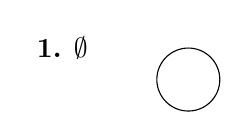
\begin{tikzpicture}[scale=0.8]
			% 1. Empty set
			\node at (0,0) {\textbf{1.} \(\emptyset\)};
			\draw (2,-0.5) circle (0.5);
		\end{tikzpicture}
		\caption*{1. Empty Set}
	\end{minipage}
	\hfill
	\begin{minipage}{0.45\textwidth}
		\centering
		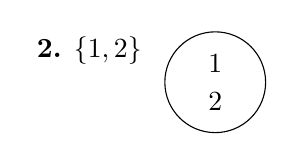
\begin{tikzpicture}[scale=0.8]
			% 2. Set with two elements
			\node at (0,0) {\textbf{2.} \(\{1,2\}\)};
			\draw (2,-0.5) circle (0.8);
			\node at (2,-0.2) {1};
			\node at (2,-0.8) {2};
		\end{tikzpicture}
		\caption*{2. Set with Two Elements}
	\end{minipage}

	\vspace{0.5cm}

	\begin{minipage}{0.45\textwidth}
		\centering
		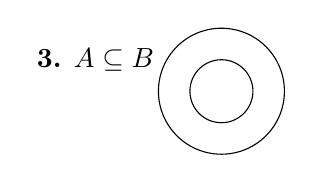
\begin{tikzpicture}[scale=0.8]
			% 3. A subset of B
			\node at (0,0) {\textbf{3.} \(A \subseteq B\)};
			\draw (2,-0.5) circle (1);
			\draw (2,-0.5) circle (0.5);
		\end{tikzpicture}
		\caption*{3. A is a subset of B}
	\end{minipage}
	\hfill
	\begin{minipage}{0.45\textwidth}
		\centering
		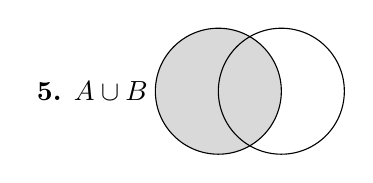
\begin{tikzpicture}[scale=0.8]
			% 5. Union
			\node at (0,0) {\textbf{5.} \(A \cup B\)};
			\begin{scope}
				\clip (2,0) circle(1);
				\fill[gray!30] (3,0) circle(1);
			\end{scope}
			\fill[gray!30] (2,0) circle(1);
			\draw (2,0) circle(1);
			\draw (3,0) circle(1);
		\end{tikzpicture}
		\caption*{5. Union of A and B}
	\end{minipage}

	\vspace{0.5cm}
\end{figure}

\newpage

\begin{figure}
	\centering
	\begin{minipage}{0.45\textwidth}
		\centering
		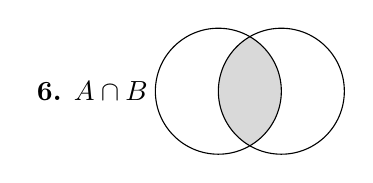
\begin{tikzpicture}[scale=0.8]
			% 6. Intersection
			\node at (0,0) {\textbf{6.} \(A \cap B\)};
			\begin{scope}
				\clip (2,0) circle(1);
				\fill[gray!30] (3,0) circle(1);
			\end{scope}
			\draw (2,0) circle(1);
			\draw (3,0) circle(1);
		\end{tikzpicture}
		\caption*{6. Intersection of A and B}
	\end{minipage}
	\hfill
	\begin{minipage}{0.45\textwidth}
		\centering
		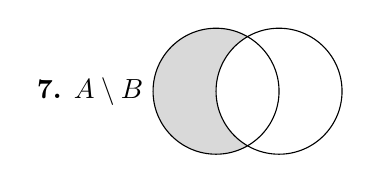
\begin{tikzpicture}[scale=0.8]
			% 7. A \ B
			\node at (0,0) {\textbf{7.} \(A \setminus B\)};
			\fill[gray!30] (2,0) circle(1);
			\begin{scope}
				\clip (3,0) circle(1);
				\fill[white] (2,0) circle(1);
			\end{scope}
			\draw (2,0) circle(1);
			\draw (3,0) circle(1);
		\end{tikzpicture}
		\caption*{7. A minus B}
	\end{minipage}

	\vspace{0.5cm}

	\begin{minipage}{0.45\textwidth}
		\centering
		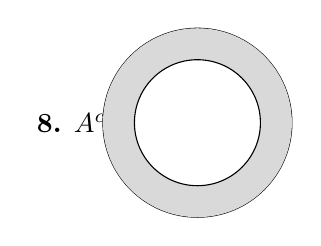
\begin{tikzpicture}[scale=0.8]
			% 8. Complement
			\node at (0,0) {\textbf{8.} \(A^c\)};
			\draw (2,0) circle(1.5);
			\fill[gray!30] (2,0) circle(1.5);
			\fill[white] (2,0) circle(1);
			\draw (2,0) circle(1);
		\end{tikzpicture}
		\caption*{8. Complement of A}
	\end{minipage}
\end{figure}
\smallskip

\subsection{Axioms of Set Theory (Zermelo Fraenkel)}
\smallskip
This are Zermelo Fraenkel axioms of set theory including \emph{The Axiom of Choice}.

\begin{enumerate}[label = \Roman*.]
	\item \emph{Axiom of Extensionality:} \quad \(\forall A, B: A = B \Rightarrow (\forall C: C \in A \Leftrightarrow C \in B)\)
	\item \emph{Empty-Set Axiom:} \quad \(\exists \emptyset : \forall X: X \notin \emptyset\)
	\item \emph{Axiom of Pairing:} \quad \(\forall A, B: \exists C: \forall D: D \in C \Leftrightarrow (D = A \lor D = B)\)
	\item \emph{Axiom of Union:} \quad \(\forall A: \exists B: \forall C: C \in B \Leftrightarrow (\exists D: C \in D \land D \in A)\)
	\item \emph{Axiom of Infinity:} \quad \(\exists N: \emptyset \in N \land (\forall x: x \in N \Rightarrow x \cup \{x\} \in N)\)
	\item \emph{Axiom Schema of Specification:} \quad \(\forall A: \exists B: \forall C: C \in B \Leftrightarrow (C \in A \land P(C))\)
	\item \emph{Axiom Schema of Replacement:} \quad \(\forall A: \exists B: \forall y: y \in B \Rightarrow \exists x \in A: y = F(x)\)
	\item \emph{Power Set Axiom:} \quad \(\forall A: \exists B: \forall C: C \subseteq A \Rightarrow C \in B\)
	\item \emph{Foundation Axiom:} \quad \(\forall A \ne \emptyset: \exists B \in A: A \cap B = \emptyset\)
	\item \emph{Axiom of Choice:} \quad \(\forall X:
		      \left( \left[ \forall A \in X: A \ne \emptyset \right] \land
		      \left[ \forall B, C \in X: B \ne C \Rightarrow B \cap C = \emptyset \right] \right) \\
		      \qquad \Rightarrow \exists Y: \forall I \in X: \exists! J \in Y: J \in I\)
\end{enumerate}

\subsection{The Cartesian Product}

The Cartesian product of two sets \(A\) and \(B\), written \(A \times B\), is the set of all ordered pairs in which the first element belongs to \(A\) and the second belongs to \(B\):
\[A \times B = \{ (a, b) : a \in A, \land\ b \in B\}.\]

\textbf{Example:}
\vspace{\baselineskip}

\begin{table}[H]
	\centering
	\caption{Cartesian Product of \(A = \{1, 2, 3\}\) and \(B = \{4, 5, 6\}\)}
	\begin{tabular}{|c|c|c|c|}
		\hline
		\multirow{3}{*}{\(A \times B\)} & \multicolumn{3}{c|}{\(b \in B\)}                       \\
		\cline{2-4}
		                              & \(4\)                            & \(5\)      & \(6\)      \\
		\hline
		\(a \in A\)                     &                                &          &          \\
		\hline
		\(1\)                           & \((1, 4)\)                       & \((1, 5)\) & \((1, 6)\) \\
		\hline
		\(2\)                           & \((2, 4)\)                       & \((2, 5)\) & \((2, 6)\) \\
		\hline
		\(3\)                           & \((3, 4)\)                       & \((3, 5)\) & \((3, 6)\) \\
		\hline
	\end{tabular}
	\label{tab:cartesian_product}
\end{table}

The general cartesian product of \emph{n} sets can be written as:
\begin{align*}
	X_{i = 1}^{n + 1} A_i & = \left( X_{i = 1}^{n} A_i \right) \times A_{n + 1} \quad \text{with} \quad X_{i = 1}^{1} A_i = A_1 \\
	\text{When } A_i      & = M \ \text{for all } i:                                                                            \\
	M^n                   & := M \times M \times \cdots \times M = X_{i = 1}^{n} M \quad \text{with} \quad M^1 = M
\end{align*}

\subsection{Laws of Set Algebra}
Let \(X\) be the universal set and \(A, B, C \subseteq X\).

\begin{itemize}[label=\(-\)]
	\item \(\emptyset \subseteq A\)
	\item \(A \subseteq B \iff A \cap B = A \iff A \cup B = B \iff X \setminus B \subseteq X \setminus A \iff B \subseteq A\)
	\item \(A \cup B = B \cup A\) \hfill (Commutative Law)
	\item \(A \cap B = B \cap A\) \hfill (Commutative Law)
	\item \((A \cup B) \cup C = A \cup (B \cup C)\) \hfill (Associative Law)
	\item \((A \cap B) \cap C = A \cap (B \cap C)\) \hfill (Associative Law)
	\item \(A \cap (B \cup C) = (A \cap B) \cup (A \cap C)\) \hfill (Distributive Law)
	\item \(A \cup (B \cap C) = (A \cup B) \cap (A \cup C)\) \hfill (Distributive Law)
	\item \(A \cup A = A \quad \text{and} \quad A \cap A = A\) \hfill (Idempotent Law)
	\item \(A \setminus B = A \cap (X \setminus B) = A \cap \overline{B}\)
	\item \(B = \overline{A} \iff (A \cup B = X \land A \cap B = \emptyset)\) \hfill (Disjoint Partition of \(X\))
	\item \(\overline{A} \cap \overline{B} = \overline{A \cup B}\) \hfill (De Morgan's Law)
	\item \(\overline{A} \cup \overline{B} = \overline{A \cap B}\) \hfill (De Morgan's Law)
	\item \(\overline{\overline{A}} = A\) \hfill (Double Negation)
\end{itemize}

\subsubsection{Proof of De Morgans's Law for sets and logic}
The complement of \( A \cup B \) is \( \overline{(A \cup B)} \), and Law (11) on disjoint decomposition states:
\[
	B = \overline{A} \iff (A \cup B = X) \land (A \cap B = \emptyset)
\]

So define \( \overline{C} := A \cup B \) and \( D := \overline{A} \cap \overline{B} \),
and use Law (11) to show the disjoint decomposition:
\[
	D = C \iff A \cap B = A \cup B
\]

To show:
\[
	D \cup C = X \iff (\overline{A} \cap \overline{B}) \cup (A \cup B) = X
\]

\begin{align*}
	(\overline{A} \cap \overline{B}) \cup (A \cup B)
	 & = (\overline{A} \cup A \cup B) \cap (\overline{B} \cup A \cup B) \quad \text{(Law (8))} \\
	 & = (X \cup B) \cap (X \cup A)                                                            \\
	 & = X \cap X                                                                              \\
	 & = X
\end{align*}

To show:
\[
	D \cap C = \emptyset \iff (\overline{A} \cap \overline{B}) \cap (A \cup B) = \emptyset
\]

\begin{align*}
	(\overline{A} \cap \overline{B}) \cap (A \cup B)
	 & = (A \cap B \cap A) \cup (A \cap B \cap B) \quad \text{(Law (7))}                      \\
	 & = (\overline{A} \cap A \cap \overline{B}) \cup (\overline{A} \cap \overline{B} \cap B) \\
	 & = (\emptyset \cap \overline{B}) \cup (\overline{A} \cap \emptyset)                     \\
	 & = \emptyset \cup \emptyset                                                             \\
	 & = \emptyset
\end{align*}

\subsection{Indexed Sets}

Let \( X \) be a set, and \( A_i \subseteq X \) for all \( i \in J \), where \( J \) is the index set.
\vspace{\baselineskip}

If \( J = \{1, 2, \dots, n\} \):
\[
	\bigcup_{i=1}^{n} A_i := A_1 \cup A_2 \cup \dots \cup A_n = \{ x \mid \exists i \in J \ (x \in A_i) \}
\]
\[
	\bigcap_{i=1}^{n} A_i := A_1 \cap A_2 \cap \dots \cap A_n = \{ x \mid \forall i \in J \ (x \in A_i) \}
\]
\[
	X_{i=1}^{n} A_i = \{(a_1, \dots, a_n) \mid a_i \in A_i \}
\]

If \( J \) is any set:
\[
	\bigcup_{i \in J} A_i := \{ x \mid \exists i \in J \ (x \in A_i) \}
\]
\[
	\bigcap_{i \in J} A_i := \{ x \mid \forall i \in J \ (x \in A_i) \}
\]

If \( J \) is any set, then \( {(A_i)}_{i \in J} \) are pairwise disjoint if and only if:
\[
	\forall i_1, i_2 \in J, \ i_1 \neq i_2 \Rightarrow A_{i_1} \cap A_{i_2} = \emptyset
\]

If \( J \) is any set, then \( {(A_i)}_{i \in J} \) forms a (disjoint) decomposition of \( X \) if and only if:
\[
	{(A_i)}_{i \in J} \text{ are pairwise disjoint and } \bigcup_{i \in J} A_i = X
\]

\subsubsection{More Partitions Laws}
Let \( A_i, B_j \subseteq X \) for \( i \in I \) and \( j \in J \). Then the following holds:

\begin{itemize}[label=\(-\)]


	\item\emph{De Morgan's Laws:}
	\[
		\overline{\bigcap_{i \in I} A_i}= \bigcup_{i \in I} \overline{A_i} \quad \text{and} \quad \overline{\bigcup_{i \in I} A_i} = \bigcap_{i \in I} \overline{A_i}
	\]

	\item\[
		\bigcap_{i \in I} A_i \cup \bigcap_{j \in J} B_j = \bigcap_{i,j} (A_i \cup B_j) \quad \text{with} \quad \bigcap_{i,j} = \bigcap_{(i,j) \in I \times J}
	\]


	\item\[
		\bigcup_{i \in I} A_i \cap \bigcup_{j \in J} B_j = \bigcup_{i,j} (A_i \cap B_j) \quad \text{with} \quad \bigcup_{i,j} = \bigcup_{(i,j) \in I \times J}
	\]

\end{itemize}

Here, \( I = \{ 1, 2, 3, \dots, n \} \) and \( J = \{ 1, 2, 3, \dots, m \} \). Then:
\[
	I \times J = \{ (i, j) \mid 1 \leq i \leq n, 1 \leq j \leq m, i, j \in \mathbb{N} \}
\]
\[
	= \{ (1, 1), (1, 2), \dots, (1, m), (2, 1), (2, 2), \dots, (2, m), \dots, (n, 1), (n, 2), \dots, (n, m) \}
\]

\subsection{Cardinality}

The cardinality of a set is the number of elements in that set.
\\
Let \( A \) and \( B \) be finite sets with \( |A| = n \), \( |B| = m \), and let \( X \) be the finite universal set. Then the following holds:

\subsubsection{Cardinality of a Set}
\[
	A = (A \cap B) \cup (A \setminus B), \quad |A| = |A \cap B| + |A \setminus B|
\]

\subsubsection{Cardinality of the complements}
\[
	|A| = |X \setminus A| = |X| - |A|
\]
\[
	A \setminus B = A \cap (X \setminus B), \quad |A \setminus B| = |A| - |A \cap B|
\]

\subsubsection{Cardinality of the Cartesian Product}
\[
	|A \times B| = |A| \cdot |B| = n \cdot m
\]

\subsubsection{Inclusion-Exclusion Formula for Two Disjoint Sets}
\[
	|A \cup B| = |A| + |B| = n + m
\]

\subsubsection{Inclusion-Exclusion Formula for Two Non-Disjoint Sets}
Let \( |A \cap B| = k \), then:
\[
	|A \cup B| = |A| + |B| - |A \cap B| = n + m - k \quad \text{(since we do not count the intersection twice)}
\]

\subsubsection{Inclusion-Exclusion Formula for Three Non-Disjoint Sets}
\[
	|A \cup B \cup C| = |(A \cup B) \cup C| = |A \cup B| + |C| - |(A \cup B) \cap C|
\]
\[
	= |A| + |B| - |A \cap B| + |C| - |(A \cap C) \cup (B \cap C)|
\]
\[
	= |A| + |B| + |C| - |A \cap B| - |A \cap C| - |B \cap C| + |A \cap B \cap C|
\]

\subsubsection{General Formula for the cardinality of the union of sets}

\[
	\left\vert \bigcup_{i = 1}^n M_i \right\vert  = \sum_{I \subseteq \{1, \dots, n\}, I \neq \emptyset}{(-1)}^{|I| - 1} \left\vert \bigcap_{i \in I} M_i \right\vert
\]

\subsection{The Power Set}
The Power Set of a set is the set of all subsets of a given set \[
	P(x):= \{ M: M \subset X\}
\]
Its cardinality is \(2^n\) with \emph{n} being the number of elements in the original set \textit{X}.

\subsection{Family of Subsets}
Let \emph{X} be a non empty set. A subset \(\mathscr{F}\) of the power set of \textit{X} is called a set system of \textit{X}

\subsection{Partition}
Let \emph{X} be a non empty set. A subset \(\mathscr{F}\) of the power set of \textit{X} is called a partition if:\\
- \(M \neq  \emptyset\ \forall M \in \mathscr{F}\)\\
- \(\bigcap \mathscr{F} = X\)\\
- \(M_1 \bigcap M_2 \ne \emptyset \implies M_1 = M_2\ \forall\ M_1, M_2 \in \mathscr{F} \)

\begin{itemize}[label=\(-\)]

	\item Every equivalence relation corresponds to a partition:
	      \[
		      J: \{ R : R\ \text{is an equivalence relation on } X\} \to \{ F: F\ \text{is a partition of } X\}
	      \]

	      where \( J(R) := X / R \) is a bijection.

	\item If \( F \) is a partition of \( X \), then we can define an equivalence relation \( R_F \) by:
	      \[
		      R_F := \{ (x, y) \in X \times X : \exists M \in F\ \text{such that } x, y \in M \}
	      \]
	      Then \( R_F \) is an equivalence relation on \( X \).

\end{itemize}


\subsection{Family of Subsets Operations}
Let \(\mathscr{F}\) be a system of sets (a family of subsets) on the set \( X \). We define:

\[
	\bigcup_{M \in F} M := \bigcup F := \{ x \in X : \text{there exists } M \in F \text{ such that } x \in M \} ,
\]

\[
	\bigcap_{M \in F} M := \bigcap F := \{ x \in X : x \in M \text{ for all } M \in F \} .
\]
\newpage
\section{Relations, Maps and Functions}

A \emph{relation} in mathematics is a connection or relationship between elements of two sets. It's 
formally defined as a subset of the Cartesian product of the sets.

For example, if we have sets \(A\) and \(B\), a relation \emph{R} from \(A\) to \(B\) consists
of ordered pairs \((a,b)\) where \(a \in A\) and \(b \in B\), such that \(a\) is related to \(b\) 
according to some rule or property.

Common types of relations include:

\begin{itemize}

	\item Functions (special relations where each input has exactly one output)

	\item Equivalence relations (reflexive, symmetric, and transitive)

	\item Partial orders (reflexive, antisymmetric, and transitive)

\end{itemize}

Relations can be represented using diagrams, matrices, or sets of
ordered pairs, and they're fundamental to many areas of mathematics including algebra, calculus, and 
discrete mathematics.

\subsection{Types of relations}

Let \(A\) be a set and \(X\) be a relation on \(A\).

\begin{itemize}

	\item \emph{Reflexive:} \(\forall a \in A: (a, a) \in X\) (or written as \(a \sim a\))

	\item \emph{Irreflexive:} \(\forall a \in A: (a, a) \not\in X\)

	\item \emph{Symmetric:} \(\forall a, b \in A: (a, b) \in X \to (b, a) \in X\) (or written as 
		  \((a \sim b) \Rightarrow (b \sim a)\))

	\item \emph{Antisymmetric:} \(\forall a, b \in A: (a, b) \in X \text{ and } (b, a) \in X \to a = b\)

	\item \emph{Transitive:} \(\forall a, b, c \in A: (a, b) \in X \text{ and } (b, c) \in X \to (a, c) 
		  \in X\) (or written as \((a \sim b) \text{ and } (b \sim c) \Rightarrow (a \sim c)\))

	\item \emph{Total:} \(\forall a,b \in A: a \neq b \to (a, b) \in X \text{ or } (b, a) \in X\)

\end{itemize}

\subsection{Equivalence relation}

An \emph{equivalence relation} is a relation that is symmetric, transitive and reflexive.

\textbf{Example:}

\[
	R:= \{ (a,b) \in \Naturals \times \Naturals: a = b\}
\]

\subsection{The Graph}

\[
	\text{graph}(f):= \{(x, f(x)): x \in X\}
\]

\subsection{The identity}

\[
	\text{id}(f):= idx:= \{(x, x): x \in X\}
\]

\subsection{Image}

The \emph{image (or range)} of a relation \emph{R} from set \(A\) to set \(B\) is the set 
of all elements in \(B\) that are related to at least one element in \(A\). Formally, if 
\(R \subseteq A \times B\) is a relation, then the image of \emph{R} is defined as:

\[
	\img(R) = \{b \in B \mid \exists a \in A \text{ such that } (a,b) \in R\}
\]

In other words, the image consists of all the output values that appear in the ordered pairs of the 
relation. For example, if \(R = \{(1,4), (2,5), (3,4), (2,6)\}\), then \(\img(R) = \{4, 5, 6\}\).

\subsection{Domain}

The \emph{domain} of a relation \emph{R} from set \(A\) to set \(B\) is the set of all elements in 
\(A\) that are related to at least one element in \(B\). Formally, if \(R \subseteq A \times B\) 
is a relation, then the domain of \emph{R} is defined as:

\[
	\text{Dom}(R) = \{a \in A \mid \exists b \in B \text{ such that } (a,b) \in R\}
\]

In other words, the domain consists of all the input values that appear in the ordered pairs of the 
relation. For example, if \(R = \{(1,4), (2,5), (3,4), (2,6)\}\), then \(\text{Dom}(R) = \{1, 2, 3\}\).

\subsection{Equivalence Class}

Let \(\sim\) be an equivalence relation on a set \(A\). For an element \(x \in A\), the 
\emph{equivalence class} of \(x\), denoted by \([x]\), is the set of all elements in \(A\) that are 
equivalent to \(x\). Formally, it is defined as:

\[
	[x] := \{y \in A \mid x \sim y\} \subseteq A
\]

In other words, the equivalence class of \(x\) contains all elements \(y\) in \(A\) such that 
\(x\) is related to \(y\) under the equivalence relation \(\sim\).

\subsection{Quotient Space}

Let \(\sim\) be an equivalence relation on a set \(A\). The \emph{quotient space} of \(A\) by 
\(\sim\), denoted by \(A/\sim\) (or sometimes \(A/R\)), is the set of all distinct equivalence classes of 
elements in \(A\). Formally, it is defined as:

\[
	A/\sim := \{[x] \mid x \in A\}
\]

The quotient space \(A/\sim\) is a partition of the original set \(A\) into disjoint equivalence classes. 
Each element of the quotient space is an equivalence class \([x]\), which itself is a subset of \(A\).

\subsection{Definition of a Map}

A map (or function) from a set \(A\) to a set \(B\), denoted as \(f: A \to B\), is a relation that 
associates each element of the set \(A\) with exactly one element of the set \(B\).

Formally, a function \(f: A \to B\) is a subset of \(A \times B\) such that for every \(a \in A\), there 
exists exactly one \(b \in B\) where \((a,b) \in f\). We typically write \(f(a) = b\) to indicate that 
\(f\) maps the element \(a\) to the element \(b\).

\textbf{Example:}

Let \(A = \{1, 2, 3\}\) and \(B = \{x, y, z\}\). A possible function \(f: A \to B\) could be defined as:

\[
	f(1) = x, \quad f(2) = y, \quad f(3) = z
\]

This function can also be represented as the set of ordered pairs \(\{(1,x), (2,y), (3,z)\}\).

\subsection{Composition of Maps}

The composition of two functions is the operation of applying one function to the result of another 
function. If we have functions \(f: A \to B\) and \(g: B \rightarrow C\), then the composition of \(g\) 
and \(f\), denoted as \(g \circ f\) (read as g composed with f), is a function from \(A\) to \(C\) defined 
by:

\[
	(g \circ f)(a) = g(f(a)) \quad \text{for all } a \in A
\]

The composition applies \(f\) first, then applies \(g\) to the result. 
Note that the co-domain of \(f\) must match the domain of \(g\) for the composition to be defined.

\textbf{Example:}

Let \(f: \Reals \to \Reals\) be defined by \(f(x) = x^2\) and \(g: \Reals \rightarrow \Reals\) be defined 
by \(g(x) = x+3\). Then:

\[
	(g \circ f)(x) = g(f(x)) = g(x^2) = x^2 + 3
\]

\[
	(f \circ g)(x) = f(g(x)) = f(x+3) = {(x+3)}^2 = x^2 + 6x + 9
\]

Note that \(g \circ f \neq f \circ g\) in general, which shows that function composition is not 
commutative.

\subsection{Types of Functions}

\subsubsection{Injective Functions}

An injective function (also called a one-to-one function) is a 
function that maps distinct elements from the domain to distinct elements in the co-domain.

Formally, a function \(f: A \to B\) is injective if for all \(a_1, a_2 \in A\):

\[
	a_1 \neq a_2 \to f(a_1) \neq f(a_2)
\]

Equivalently, using the contrapositive:

\[
	f(a_1) = f(a_2) \to a_1 = a_2
\]

\subsubsection{Surjective Functions}

A surjective function (also called an onto function) is a function whose image equals its co-domain, 
meaning that every element in the co-domain has at least one pre-image in the domain.

Formally, a function \(f: A \to B\) is surjective if:

\[
	\forall b \in B, \exists a \in A \text{ such that } f(a) = b
\]

\subsubsection{Bijection Functions}

A bijective function (also called a one-to-one correspondence) is a 
function that is both injective and surjective. In other words, every 
element in the co-domain is mapped to by exactly one element in the domain.

Formally, a function \(f: A \to B\) is bijective if it is both:

\begin{itemize}

	\item Injective: \(\forall a_1, a_2 \in A, a_1 \neq a_2 \to f(a_1) \neq f(a_2)\)

	\item Surjective: \(\forall b \in B, \exists a \in A \text{ such that } f(a) = b\)

\end{itemize}

Bijective functions establish a perfect pairing between elements of the domain and co-domain, where each 
element in the domain corresponds to exactly one element in the co-domain, and vice versa. A bijection 
allows us to define an inverse function \(f^{-1}: B \to A\).

\subsection{Propositions on Images and Pre-images under Set Operations}

Let \( f : X \to Y \) be a function.

\subsubsection{Union and Cut Sets}

\begin{itemize}

	\item For subsets \( A_1, A_2 \subseteq X \), we have:

	      \[
		      f(A_1 \cup A_2) = f(A_1) \cup f(A_2)
		      \quad \text{and} \quad
		      f(A_1 \cap A_2) \subseteq f(A_1) \cap f(A_2)
	      \]

	\item For subsets \( B_1, B_2 \subseteq Y \), we have:
	      
	      \[
		      f^{-1}(B_1 \cup B_2) = f^{-1}(B_1) \cup f^{-1}(B_2)
		      \quad \text{and} \quad
		      f^{-1}(B_1 \cap B_2) = f^{-1}(B_1) \cap f^{-1}(B_2)
	      \]
\end{itemize}

\textbf{Proof:}

We prove the second part of 1 and the first part of 2.

Let \( y \in f(A_1 \cap A_2) \). Then there exists \( x \in A_1 \cap A_2 \) such that 
\( f(x) = y \). Since \( x \in A_1 \) and \( x \in A_2 \), it follows that \( y \in f(A_1) \) 
and \( y \in f(A_2) \), hence \( y \in f(A_1) \cap f(A_2) \). Therefore, every element of 
\( f(A_1 \cap A_2) \) is also an element of \( f(A_1) \cap f(A_2) \), so:

\[
	f(A_1 \cap A_2) \subseteq f(A_1) \cap f(A_2)
\]

Let \( x \in f^{-1} (B_1 \cup B_2) \). Then \( f(x) \in B_1 \cup B_2 \), which means \( f(x) \in B_1 \) 
or \( f(x) \in B_2 \). Thus, \( x \in f^{-1}(B_1) \) 
or \( x \in f^{-1}(B_2) \), which implies:
	      
\[
	 x \in f^{-1}(B_1) \cup f^{-1}(B_2)
\]

Hence, both sets contain the same elements and are therefore, equal:
	      
\[
	f^{-1}(B_1 \cup B_2) = f^{-1}(B_1) \cup f^{-1}(B_2)
\]

\QED

\subsubsection{Union and Cut of the whole Domain and Range}

Let \( f : X \to Y \) be a function.

\begin{itemize}

	\item Let \( \mathcal{F} \) be a collection of subsets of \(X\). Then:

   	      \[
		      f\left( \bigcup_{A \in \mathcal{F}} A \right) = \bigcup_{A \in \mathcal{F}} f(A)
		      \quad \text{and} \quad
		      f\left( \bigcap_{A \in \mathcal{F}} A \right) \subseteq \bigcap_{A \in \mathcal{F}} f(A)
	      \]

	\item Let \( \mathcal{G} \) be a collection of subsets of \emph{Y}. Then:

	      \[
		      f^{-1}\left( \bigcup_{B \in \mathcal{G}} B \right) = \bigcup_{B \in \mathcal{G}} f^{-1}(B)
		      \quad \text{and} \quad
		      f^{-1}\left( \bigcap_{B \in \mathcal{G}} B \right) = \bigcap_{B \in \mathcal{G}} f^{-1}(B)
	      \]

\end{itemize}

\textbf{Proof (partial):}

We show the first statement of part (ii); the rest follows analogously.

Let \( x \in f^{-1} \left( \bigcup_{B \in \mathcal{G}} B \right) \). Then:

\[
	f(x) \in \bigcup_{B \in \mathcal{G}} B
	\quad \Leftrightarrow \quad
	\exists B \in \mathcal{G} \text{ such that } f(x) \in B
	\quad \Leftrightarrow \quad
	\exists B \in \mathcal{G} \text{ such that } x \in f^{-1}(B)
\]

Hence:

\[
	x \in \bigcup_{B \in \mathcal{G}} f^{-1}(B)
\]

It follows that:

\[
	f^{-1} \left( \bigcup_{B \in \mathcal{G}} B \right) = \bigcup_{B \in \mathcal{G}} f^{-1}(B)
\]

\QED

\subsection{Inverse of a Function}

The \emph{inverse} of a function \(f: A \to B\) is a function \(f^{-1}: B \to A\) that 
reverses the operation of \(f\). That is, if \(f\) maps an element \(a \in A\) to an 
element \(b \in B\), then the inverse function \(f^{-1}\) maps \(b\) back to \(a\).

Formally, a function \(f: A \to B\) has an inverse \(f^{-1}: B \to A\)  
if and only if \(f\) is bijective (both injective and surjective). The inverse function satisfies the 
following properties:

\[
	f^{-1}(f(a)) = a \quad \text{for all } a \in A
\]

\[
	f(f^{-1}(b)) = b \quad \text{for all } b \in B
\]

In other words, composing a function with its inverse yields the identity function. That is:

\[
	f^{-1} \circ f = id_A \quad \text{and} \quad f \circ f^{-1} = id_B
\]

Where \(id_A\) and \(id_B\) are the identity functions on sets \(A\) and \(B\), respectively.

\subsubsection{Steps to Find the Inverse of a Function}

To find the inverse of a function \(f (x)\), follow these steps:

\begin{enumerate}
	
	\item Replace \(f (x)\) with \(y\): \(y = f (x)\)
	
	\item Interchange the variables \(x\) and \(y\): \(x = f (y)\)
	
	\item Solve for \(y\) in terms of \(x\): \(y = f^{-1} (x)\)
	
	\item Verify that the resulting function is indeed the inverse by checking that \(f^{-1}(f(x)) = x\) 
		  and \(f (f^{-1} (x)) = x\)

		\end{enumerate}

\textbf{Example:}

Let's apply the steps above to find the inverse of \(f (x) = 2x + 3\).

\textbf{Step 1: Replace \(f(x)\) with \(y\)}

\[
	y = 2x + 3
\]

\textbf{Step 2: Interchange the variables \(x\) and \(y\)}

\[
	x = 2y + 3
\]

\textbf{Step 3: Solve for \(y\) in terms of \(x\)}

\begin{align*}
	x               & = 2y + 3 \\
	x - 3           & = 2y     \\
	\frac{x - 3}{2} & = y
\end{align*}

So, the inverse function is:

\[
	f^{-1}(x) = \frac{x - 3}{2}
\]

\textbf{Step 4: Verify that \(f^{-1} (f (x)) = x\) and \(f(f^{-1} (x)) = x\)}

Let's verify \(f^{-1} (f (x)) = x\):

\begin{align*}
	f^{-1}(f(x)) & = f^{-1}(2x + 3)         \\
	             & = \frac{(2x + 3) - 3}{2} \\
	             & = \frac{2x}{2}           \\
	             & = x
\end{align*}

And let's verify \(f(f^{-1}(x)) = x\):

\begin{align*}
	f(f^{-1}(x)) & = f\left(\frac{x - 3}{2}\right)     \\
	             & = 2\left(\frac{x - 3}{2}\right) + 3 \\
	             & = (x - 3) + 3                       \\
	             & = x
\end{align*}

Since both compositions yield the identity function, \(f^{-1} (x) = \frac{x - 3}{2}\) is indeed the 
inverse of \(f (x) = 2x + 3\).

\subsubsection{Properties of the Inverse Function}

Let \(f:X\to Y\) be a function.

\begin{itemize}

	\item Assume \(x \sim y \) if \(f(x)= f(y)\) so is \(\sim\) an equivalence relation.

	\item Consider the quotient set \( X_f := X/\sim \), where \( \sim \) is the equivalence relation 
	      defined by \( x \sim x' \iff f(x) = f(x') \). Let \( q_f : X \to X_f \) be the canonical 
		  projection defined by \( q_f(x) = [x] \), and let \( \iota_f : f(X) \to Y \) be the inclusion  
		  map, \( y \mapsto y \). Then the function
	      
		  \[
		      \hat{f} : X_f \to f(X), \quad [x] \mapsto f(x)
	      \]
	  
		  is a bijection, and the original map \(f\) can be written as the composition
	 
		  \[
		      f = \iota_f \circ \hat{f} \circ q_f.
	      \]
	 
		  Here, \( q_f \) is surjective, \( \hat{f} \) is bijective, and \( \iota_f \) is injective. 
		  This yields the following commutative diagram:
	      
		  \begin{center}
				\begin{tikzcd}
					X \arrow[r, "f"] \arrow[d, "q_f"] & Y                         \\
					X_f \arrow[r, "\hat{f}"]          & f(X) \arrow[u, "\iota f"]
				\end{tikzcd}
	      \end{center}

\end{itemize}

\subsection{Transformations of a Function}

Transformations modify the appearance of a function's graph without altering its basic shape.
Here, we examine how different algebraic changes to a function \( f(x) \) affect its graph:

\emph{Vertical Translation:} \( f(x) + a \)
	    
\begin{itemize}
	
	\item Shifts the graph \emph{upward} if \( a > 0 \), and \emph{downward} if \( a < 0 \).
	
	\item Each point on the graph moves vertically by \(a\) units.

\end{itemize}

\emph{Horizontal Translation:} \( f(x + a) \)

\begin{itemize}

	\item Shifts the graph \emph{left} if \( a > 0 \), and \emph{right} if \( a < 0 \).

	\item This is opposite of what might be expected: adding to \(x\) shifts the graph in the negative 
	      direction.

\end{itemize}

\emph{Vertical Scaling (Stretch/Compression):} \( a f(x) \)

\begin{itemize}
	
	\item If \( |a| > 1 \): the graph is \emph{stretched} vertically (taller and narrower).
	
	\item If \( 0 < |a| < 1 \): the graph is \emph{compressed} vertically (shorter and wider).
	
	\item If \( a < 0 \): includes a reflection across the \emph{x-axis}.

\end{itemize}

\emph{Horizontal Scaling (Stretch/Compression):} \( f(a x) \)

\begin{itemize}

	\item If \( |a| > 1 \): the graph is \emph{compressed} horizontally (narrower).

	\item If \( 0 < |a| < 1 \): the graph is \emph{stretched} horizontally (wider).

	\item If \( a < 0 \): includes a reflection across the \emph{y-axis}.

\end{itemize}

\emph{Reflection across the x-axis:} \( -f(x) \)
	
\begin{itemize}

	\item Flips the graph upside-down over the x-axis.

	\item Each point \( (x, y) \) becomes \( (x, -y) \).

\end{itemize}

\emph{Reflection across the y-axis:} \( f(-x) \)

\begin{itemize}

	\item Flips the graph left-to-right over the y-axis.

	\item Each point \( (x, y) \) becomes \( (-x, y) \).

\end{itemize}


\newpage
\section{Mathematical Proofs}

In this section I will provide with some examples of different types of proofs.

\subsection{Proof by Direct Argument}

For any integer \( n \), if \( n \) is even, then \( n^2 \) is even.
\vspace{\baselineskip}

We will prove this theorem by direct argument.
\vspace{\baselineskip}

Assume \( n \) is an even integer. Then we can write \( n = 2k \) for some integer \( k \).
\vspace{\baselineskip}

Now, we compute \( n^2 \):

\[		
	n^2 = {(2k)}^2 = 4k^2 = 2(2k^2)
\]
	
This shows that \( n^2 \) is even, as it can be expressed as \( 2m \) where \( m = 2k^2 \) is an integer.
Therefore, we conclude that if \( n \) is even, then \( n^2 \) is even.

\QED

\subsection{Proof by Contradiction}

If \( n \) is an integer such that \( n^2 \) is even, then \( n \) is even.
\vspace{\baselineskip}

We will prove this theorem by contradiction. Assume that \( n \) is an integer such that \( n^2 \) is even, but \( n \) is odd. Then we can write \( n = 2k + 1 \) for some integer \( k \).
\vspace{\baselineskip}

Now, we compute \( n^2 \):

\[
	n^2 = {(2k + 1)}^2 = 4k^2 + 4k + 1 = 2(2k^2 + 2k) + 1
\]
	
This shows that \( n^2 \) is odd, which contradicts our assumption that \( n^2 \) is even. Therefore, our assumption that \( n \) is odd must be false, and thus, \( n \) must be even.

\QED

\subsection{Proof by Induction}

For all \( n \in \Naturals \), the sum of the first \( n \) positive integers is given by:
\[
	S(n) = 1 + 2 + 3 + \cdots + n = \frac{n(n+1)}{2}
\]
We will prove this theorem by induction on \( n \).
\vspace{\baselineskip}

\textbf{Base Case:} For \( n = 1 \):

\[
	S(1) = 1 = \frac{1(1+1)}{2}
\]

The base case holds.
\vspace{\baselineskip}

\textbf{Inductive Step:} Assume that the statement holds for some \( n = k \), i.e., assume that:
	
\[
	S(k) = 1 + 2 + 3 + \cdots + k = \frac{k(k+1)}{2}
\]
	
We need to show that the statement holds for \( n = k + 1 \):

\[
	S(k+1) = S(k) + (k + 1)
\]
	
By the inductive hypothesis, we have:

\begin{align*}
	S(k+1) &= \frac{k(k+1)}{2} + (k + 1) \\
	&= \frac{k(k+1)}{2} + \frac{2(k + 1)}{2}\\
    &= \frac{k(k+1) + 2(k + 1)}{2} \\
	&= \frac{(k + 1)(k + 2)}{2}	
\end{align*}

Thus, the statement holds for \( n = k + 1 \).
By the principle of mathematical induction, the statement holds for all \( n \in \Naturals \).

\QED

\subsection{Proof by Exhaustion}

The only integer solutions to the equation \( x^2 + y^2 = 1 \) are \( (0, 1), (1, 0), (0, -1), (-1, 0) \).
\vspace{\baselineskip}

We will prove this theorem by exhaustion. We will check all possible integer values of \( x \) and \( y \) such that \( x^2 + y^2 = 1 \).
\vspace{\baselineskip}

The possible integer values for \( x \) and \( y \) are \( -1, 0, 1 \). We will check each case:
\vspace{\baselineskip}

If \( x = 0 \):
\vspace{\baselineskip}

Then \( y^2 = 1 \) gives \( y = 1 \) or \( y = -1 \).
\vspace{\baselineskip}

Solutions: \( (0, 1), (0, -1) \).
\vspace{\baselineskip}

If \( x = 1 \):
\vspace{\baselineskip}

Then \( y^2 = 0 \) gives \( y = 0 \).
\vspace{\baselineskip}

Solution: \( (1, 0) \).
\vspace{\baselineskip}

If \( x = -1 \):
\vspace{\baselineskip}

Then \( y^2 = 0 \) gives \( y = 0 \).
\vspace{\baselineskip}

Solution: \( (-1, 0) \).
\vspace{\baselineskip}

Thus, the only integer solutions to the equation are:
	
\[
	(0, 1), (1, 0), (0, -1), (-1, 0)
\]

\QED

\subsection{Proof by Cases}

For any integer \( n \), \( n^2 \) is even if and only if \( n \) is even.
\vspace{\baselineskip}

We will prove this theorem by cases.
\vspace{\baselineskip}

\textbf{Case 1:} Assume \( n \) is even. Then we can write \( n = 2k \) for some integer \( k \).
\vspace{\baselineskip}

Now, we compute \( n^2 \):

\[
	n^2 = {(2k)}^2 = 4k^2 = 2(2k^2)
\]

This shows that \( n^2 \) is even.
\vspace{\baselineskip}

\textbf{Case 2:} Assume \( n \) is odd. Then we can write \( n = 2k + 1 \) for some integer \( k \).
\vspace{\baselineskip}

Now, we compute \( n^2 \):

\[
	n^2 = {(2k + 1)}^2 = 4k^2 + 4k + 1 = 2(2k^2 + 2k) + 1
\]

This shows that \( n^2 \) is odd.
\vspace{\baselineskip}

Since both cases have been considered, we conclude that \( n^2 \) is even if and only if \( n \) is even.

\QED

\subsection{Proof by Construction}

There exists an irrational number \( x \) such that \( x^2 \) is rational.
\vspace{\baselineskip}

We will construct an irrational number \( x \) such that \( x^2 \) is rational.
\vspace{\baselineskip}

Let \( x = \sqrt{2} \). We know that \( \sqrt{2} \) is irrational. Now, we compute \( x^2 \):
	
\[
	x^2 = (\sqrt{2})^2 = 2
\]
	
Since \( 2 \) is a rational number, we have constructed an irrational number \( x = \sqrt{2} \) such that \( x^2 = 2 \) is rational.
Therefore, the theorem is proved.

\QED

\subsection{Proof by Counterexample}

The statement all prime numbers are odd is false.
\vspace{\baselineskip}

To prove this theorem, we will provide a counterexample.
\vspace{\baselineskip}

The number \( 2 \) is a prime number, as its only divisors are \( 1 \) and \( 2 \). However, \( 2 \) is even, which contradicts the statement that all prime numbers are odd.
\vspace{\baselineskip}

Therefore, the statement All prime numbers are odd is false.
\QED

\subsection{Proof by Contrapositive}

If \( n \) is an integer such that \( n^2 \) is odd, then \( n \) is odd.
\vspace{\baselineskip}

We will prove this theorem by contrapositive. The contrapositive of the statement is: If \( n \) is an integer such that \( n \) is even, then \( n^2 \) is even.
\vspace{\baselineskip}

Assume \( n \) is even. Then we can write \( n = 2k \) for some integer \( k \).
\vspace{\baselineskip}

Now, we compute \( n^2 \):
	
\[
	n^2 = {(2k)}^2 = 4k^2 = 2(2k^2)
\]

This shows that \( n^2 \) is even.
\vspace{\baselineskip}

Since the contrapositive statement is true, the original statement If \( n^2 \) is odd, then \( n \) is odd is also true.

\QED

\subsection{Proof by Reduction to Absurdity}

The square root of \( 2 \) is irrational.
\vspace{\baselineskip}

We will prove this theorem by reduction to absurdity. Assume that \( \sqrt{2} \) is rational. Then we can write:

\[
	\sqrt{2} = \frac{p}{q}
\]

Where \( p \) and \( q \) are integers with no common factors (i.e., the fraction is in the simplest form).
\vspace{\baselineskip}

Squaring both sides gives:

\[
	2 = \frac{p^2}{q^2}
\]
	
Rearranging gives:

\[
	p^2 = 2q^2
\]
	
This implies that \( p^2 \) is even, and therefore, \( p \) must be even (since the square of an odd number is odd).
Let \( p = 2k \) for some integer \( k \). Substituting this back into the equation gives:

\begin{align*}
{(2k)}^2 &= 2q^2\\	
4k^2 &= 2q^2\\
2k^2 &= q^2
\end{align*}

This implies that \( q^2 \) is even, and therefore, \( q \) must also be even.
Since both \( p \) and \( q \) are even, they have a common factor of \( 2 \), which contradicts our assumption that \( p \) and \( q \) have no common factors.
Therefore, our assumption that \( \sqrt{2} \) is rational must be false, and thus, \( \sqrt{2} \) is irrational.

\QED

\subsection{Proof by Analogy}

The set of rational numbers is dense in the set of real numbers.

We will prove this theorem by analogy.
\vspace{\baselineskip}
	
Consider the set of rational numbers \( \Rationals \) and the set of real numbers \( \Reals \). The density of \( \Rationals \) in \( \Reals \) means that between any two real numbers, there exists a rational number.
For example, between the real numbers \( 1 \) and \( 2 \), we can find the rational number \( \frac{3}{2} = 1.5 \). Similarly, between any two real numbers \( a \) and \( b \) (where \( a < b \)), we can find a rational number \( r = \frac{a + b}{2} \).
\vspace{\baselineskip}

This shows that the set of rational numbers is dense in the set of real numbers.
Therefore, the theorem is proved by analogy.

\QED




\newpage
\section{The Natural Numbers}

In this section we will take a look at the natural numbers, which are the numbers we use for counting. 
The natural numbers are defined as follows:
\vspace{\baselineskip}

We will now define the set of natural numbers, \( \Naturals \), via the following 9 axioms. 
These axioms are known as the \emph{Peano Axioms}. The first 4 axioms define equality on 
the set \( \Naturals \).

\begin{enumerate}[label=\Roman*.]

	\item For every \( x \in \Naturals \), we have \( x = x \).\hfill (Reflexivity)
	
	\item For every \( x, y \in \Naturals \), if \( x = y \) then \( y = x \).\hfill (Symmetry)
	
	\item For every \( x, y, z \in \Naturals \), if \( x = y \) and \( y = z \) then \( x = z \).\hfill 
	      (Transitivity)
	
	\item For all \( x, y \), if \( x \in \Naturals \) and \( x = y \), then \( y \in \Naturals \).\hfill 
	      (Closure of Equality)

\end{enumerate}

The remaining 5 axioms define the structure of \( \Naturals \):

\begin{enumerate}[label=\Roman*.]
	\setcounter{enumi}{4}

	\item \( 1 \in \Naturals \)
	
	\item If \( x \in \Naturals \), then the successor \( S(x) \in \Naturals \).
	
	\item There is no \( x \in \Naturals \) such that \( S(x) = 1 \).
	
	\item For all \( x, y \in \Naturals \), if \( S(x) = S(y) \), then \( x = y \).
	
	\item Let \( P(x) \) be a statement about the natural number \emph{x}. If:
	
		\begin{itemize}
	
			\item \( P(1) \) is true, and
	
			\item for all \( n \in \Naturals \), if \( P(n) \) is true, then \( P(S(n)) \) is also true,
	
		\end{itemize}
	
		then \( P(x) \) is true for all \( x \in \Naturals \).\hfill (Mathematical Induction)
\end{enumerate}

As shorthand, we denote:

\[
	S(1) = 2, \quad S(S(1)) = 3, \quad S(S(S(1))) = 4, \quad \text{and so on.}
\]

\subsection{Order in Fields}

An \emph{ordered field} is a field \emph{F} equipped with a total order \( < \) that is compatible with 
the field operations + and \( \cdot \). That is, the order satisfies both algebraic and ordering 
properties.

\subsubsection{Order Axioms for Fields}

A field \emph{F} is called an \emph{ordered field} if it satisfies the following properties for all 
\( a, b, c \in F \):

\begin{enumerate}[label=\Roman*.]
    
	\item \emph{Trichotomy:} Exactly one of the following holds:
 
		  \[
 	   			a < b, \quad a = b, \quad a > b
    	   \]

    \item \emph{Transitivity:} If \( a < b \) and \( b < c \), then \( a < c \).

    \item \emph{Additive Compatibility:} If \( a < b \), then \( a + c < b + c \).

    \item \emph{Multiplicative Compatibility:} If \( 0 < a \) and \( 0 < b \), then \( 0 < ab \).

\end{enumerate}

These properties ensure that arithmetic operations respect the order structure.

\subsubsection{Consequences of the Order Axioms}

\begin{itemize}

	\item \( a < b \Rightarrow -b < -a \)

	\item \( a < b \land c < 0 \Rightarrow ac > bc \)

	\item Squares are always non-negative: \( a^2 \ge 0 \)

	\item The order is total: any two elements are comparable

\end{itemize}

\subsubsection{Examples of Ordered Fields}

\begin{itemize}

	\item \( \Rationals \): Rational numbers with the usual order

	\item \( \Reals \): Real numbers with the usual order

	\item \( \Complex \): Complex numbers are \textbf{not} an ordered field, since \( i^2 = -1 < 0 \) 
	      would violate positivity of squares

\end{itemize}

\subsection{Propositions and Proofs}

\subsubsection{Proposition 1: \texorpdfstring{\(n \ne m \implies S(n) \ne S(m)\)}{n!= m implies S (n)!=S (m)}}

\textbf{Proof:} 

We will prove this by contradiction. Assume \( n \ne m \) and \( S(n) = S(m) \). 
By Axiom 8, we have \( n = m \), which is a contradiction. Therefore, \( S(n) \ne S(m) \).

\subsubsection{Proposition 2: \texorpdfstring{\text{For any} \(n \in \Naturals,\ n \ne S(n)\)}{ For any n in N, n!= S (n)}}

\textbf{Proof:} 

\(M = \{n \in \Naturals \| n \ne S(n) \}\ \)

By \(1 \ne S(n)\ \) for any \(n \in \Naturals\), this implies that 1 is part of the set \emph{M}. 
This implies that \(S(n) \ne S(S(n)) \implies S(n) \in M\ \) By Axiom 9 \(M = \Naturals\)

\subsubsection{Proposition 3: \texorpdfstring{\(n \ne 1\ \exists m \in \Naturals \mid n = S(m)\)}{n!= 1, exists m in N | n = S (m)}}

\textbf{Proof:}

\[
	M = \{1\} \cup\{n \in \Naturals | \text{Proposition 3 is true}\}
\]

We know that 1 ins in the set \emph{M}. And by proposition 1 we know that

\[
	S(n) = S(S(m)) \implies S(n) \in M
\]

And by Axiom 9 we know that \(M = \Naturals\)

\subsection{Definition of Addition in \texorpdfstring{\(\Naturals\)}{}}

For any pair n, m \(\in \Naturals\) there is a unique way to define

\[
	\text{Add}(n , m) = n + m
\]

\begin{enumerate}
	
	\item \textbf{Base Case:} \(n + 1 = S(n)\)

	\item \textbf{Inductive Step:} \(n + S(m) = S(n + m) \iff S(n + m)\)

\end{enumerate}

\textbf{Uniqueness:} 
\vspace{\baselineskip}

Suppose: \textit{A} \& \textit{B} satisfy our conditions. Fix n and then let \(M = \{ m \in \Naturals | 
A(n,m) = B(n, m)\}\). Then

\[
	A(n,1) = S(n) = B(n,1) \implies 1 \in M
\]

\[
	m \in M \implies A(n, m) = B(n, m) \implies A(n, S(m)) = S(A(n, m)) = S(B(n, m)) = B(n, S(m))
\]

\[
	\implies A(n , S(m)) = B(n, S(m))
\]

by Axiom 9 we know that \(M = \Naturals\) and A = B

\textbf{Construction:} For \(n = 1\) Define \(A(n, m) = S(m)\)

\begin{enumerate}
	
	\item \(A(n, 1) = S(n) = S(1)\)
	
	\item \(A(n, S(m)) = S(A(n, m)) = S(S(m))\)

\end{enumerate}

Define: \(A(S(n), S(m)) = S(A(n, m))\)

\begin{enumerate}

	\item \(A(S(n), 1) = S(A(n, 1)) = S(S(n))\)

	\item \(A(S(n), S(m)) = S(A(n, m)) = S(S(m))\)

\end{enumerate}

\textbf{Commutativity of Addition:}
\vspace{\baselineskip}

The proposition says \(n + m = m + n\) for any \(n, m \in \Naturals\). We will prove this by 
induction on \(m\). Fix n and consider \(M = \{ n \in \Naturals | A(n, m) = A(n, m)\}\)

Now recall that \(A(n, 1) = S(n)\)
\vspace{\baselineskip}

For \(n = 1\):

\[
	A(n, 1) = S(1) = A(1, n) \implies 1 \in \Naturals
\]

also \(A(n , k) = 1 + k \implies 1 + m = S(m) \implies 1 + m = m + 1 \implies 1 \in \Naturals\)

Suppose: \(n \in \Naturals \implies n + m = m + n\) or \(A(n, m) = A(m, n)\)

By construction \(A(S(n), m) = S(A(n, m))\) and by definition
\(A(S(n), m) = S(A(n, m)) = A(m, S(n)) = S(n) + m =  m + S(n) \implies S(n) \in M \implies 
\text{by induction } M = \Naturals\).

\newpage
\section{The Archimedean Principle}

For any real number \( x \in \mathbb{R} \), there exists a natural number \( n \in \mathbb{N} \) such that \( n > x \).
\\\\
In other words, no matter how large a real number you choose, there is always a natural number that is larger. Similarly, for any positive real number \( \epsilon > 0 \), there exists a natural number \( n \in \mathbb{N} \) such that \( \frac{1}{n} < \epsilon \).

\textbf{Proof:}

We prove the Archimedean Principle by contradiction.
\\\\
Assume that there exists some real number \( x \in \mathbb{R} \) such that \( n \leq x \) for all \( n \in \mathbb{N} \). That is, \( x \) is an upper bound for the set \( \mathbb{N} \subset \mathbb{R} \).

Let \( S = \sup(\mathbb{N}) \), the least upper bound of \( \mathbb{N} \). Then \( S - 1 < \sup(\mathbb{N}) \), so \( S - 1 \) is not an upper bound of \( \mathbb{N} \). Hence, there exists \( n_0 \in \mathbb{N} \) such that:
\[
	n_0 > S - 1 \Rightarrow n_0 + 1 > S
\]
But \( n_0 + 1 \in \mathbb{N} \), which contradicts the assumption that \( S \) is an upper bound of \( \mathbb{N} \). Therefore, our assumption must be false, and the theorem is proven.

\QED

\subsection{Equivalent Formulations}

The Archimedean Principle is often stated in different but equivalent ways:

\begin{itemize}[label=\(-\)]
	\item For any \( \epsilon > 0 \), there exists \( n \in \mathbb{N} \) such that \( \frac{1}{n} < \epsilon \).
	\item For any \( a, b \in \mathbb{R} \) with \( a > 0 \), there exists \( n \in \mathbb{N} \) such that \( na > b \).
\end{itemize}

\subsection{Applications}

\begin{enumerate}
	\item \textbf{Density of Rational Numbers:} The Archimedean Principle helps in proving that between any two real numbers, there exists a rational number.

	\item \textbf{Limits and Infinitesimals:} It ensures that sequences like \( \left\{ \frac{1}{n} \right\} \) converge to 0, foundational in real analysis and calculus.

	\item \textbf{Bounding Functions:} It is used in analysis to show that functions do not grow faster than natural numbers in certain contexts.

	\item \textbf{Non-Existence of Infinitely Small Numbers:} The principle implies that real numbers do not contain infinitesimals (nonzero numbers smaller than all \( \frac{1}{n} \)), distinguishing \( \mathbb{R} \) from non-standard number systems.
\end{enumerate}


\section{Fundamental Theorem of Arithmetic}

\begin{itemize}[label=\(-\)]
	\item The Fundamental Theorem of Arithmetic says that every integer greater than 1 can be factored uniquely into a product of primes.
	\item Euclid’s lemma says that if a prime divides a product of two numbers, it must divide at least one of the numbers.
	\item The least common multiple \([a, b]\) of nonzero integers \(a\) and \(b\) is the smallest positive integer divisible by both \(a\) and \(b\).
\end{itemize}

\subsection{Fundamental Theorem of Arithmetic}

Every integer greater than 1 can be written in the form
\[
	p_1^{n_1}p_2^{n_2} \cdots p_k^{n_k}
\]
where \(n_i \geq 0\) and the \(p_i\) are distinct primes. The factorization is unique, except possibly for the order of the factors.

\textbf{Example.}
\[
	4312 = 2 \cdot 2156 = 2 \cdot 2 \cdot 1078 = 2 \cdot 2 \cdot 2 \cdot 539 = 2 \cdot 2 \cdot 2 \cdot 7 \cdot 77 = 2 \cdot 2 \cdot 2 \cdot 7 \cdot 7 \cdot 11
\]
That is,
\[
	4312 = 2^3 \cdot 7^2 \cdot 11
\]

\subsection{Lemmas}

\textbf{Lemma} 

If \(m \mid pq\) and \(\gcd(m, p) = 1\), then \(m \mid q\).

\textbf{Proof:} 

Write \(1 = \gcd(m, p) = am + bp\) for some \(a, b \in \mathbb{Z}\).
Then
\[
	q = amq + bpq
\]
Since \(m \mid amq\) and \(m \mid bpq\) (because \(m \mid pq\)), we conclude \(m \mid q\).

\QED


\textbf{Lemma} 

If \(p\) is prime and \(p \mid a_1a_2 \cdots a_n\), then \(p \mid a_i\) for some \(i\).

\textbf{Proof (Case \(n=2\)):} 

Suppose \(p \mid a_1a_2\), and \(p \nmid a_1\).
Then \(\gcd(p, a_1) = 1\), and by the previous lemma, \(p \mid a_2\).

For general \(n > 2\): Assume the result is true for \(n-1\). Suppose \(p \mid a_1a_2 \cdots a_n\).
Group as \((a_1a_2 \cdots a_{n-1})a_n\).

By the \(n=2\) case, either \(p \mid a_n\) or \(p \mid a_1a_2 \cdots a_{n-1}\), and by induction, \(p \mid a_i\) for some \(i\).

\QED

\subsection{Proof of the Fundamental Theorem}

\textbf{Existence:}

Use induction on \(n > 1\).
Base case: \(n = 2\) is prime.

Inductive step: If \(n\) is prime, done. Otherwise \(n = ab\), with \(1 < a, b < n\).
By induction, both \(a\) and \(b\) factor into primes, so \(n\) does too.

\textbf{Uniqueness:}

Suppose:
\[
	p_1^{m_1} \cdots p_j^{m_j} = q_1^{n_1} \cdots q_k^{n_k}
\]
with all \(p_i\) and \(q_i\) distinct primes.

Since \(p_1\) divides the LHS, it divides the RHS. So \(p_1 \mid q_i^{n_i}\) for some \(i\), hence \(p_1 = q_i\).
Reorder so \(p_1 = q_1\). Then:

If \(m_1 > n_1\), divide both sides by \(q_1^{n_1}\):
\[
	p_1^{m_1-n_1} \cdots p_j^{m_j} = q_2^{n_2} \cdots q_k^{n_k}
\]
But then \(p_1\) divides LHS but not RHS, contradiction. So \(m_1 = n_1\). Cancel and repeat.

Eventually, all \(p_i\) match with some \(q_i\), and the exponents are equal. So the factorizations are the same up to order.

\QED

\subsection{Least Common Multiple}

The least common multiple of \(a\) and \(b\), denoted \([a, b]\), is the smallest positive integer divisible by both.

\textbf{Example:}
\[
	[6, 4] = 12, \quad [33, 15] = 165
\]

\textbf{Fact:}
\[
	[a, b] \cdot \gcd(a, b) = ab
\]

Let:
\[
	a = p_1 \cdots p_lq_1 \cdots q_m, \quad b = q_1 \cdots q_mr_1 \cdots r_n
\]

Then:
\begin{align*}
	\gcd(a, b) & = q_1 \cdots q_m                                 \\
	[a, b]     & = p_1 \cdots p_lq_1 \cdots q_mr_1 \cdots r_n     \\
	ab         & = p_1 \cdots p_lq_1^2 \cdots q_m^2r_1 \cdots r_n
\end{align*}
So:
\[
	[a, b] \cdot \gcd(a, b) = ab
\]

\textbf{Example:}
\[
	\gcd(36, 90) = 18, \quad [36, 90] = 180, \quad 36 \cdot 90 = 32400 = 18 \cdot 180
\]

\newpage
\section{Real Numbers}

Let \( K \) be an ordered field.

On the set
		\[
			\operatorname{ch}(K) := \{ x : \mathbb{N} \to K \mid x \text{ is a Cauchy sequence} \}
		\]
		and on the set
		\[
			c(K) := \{ x : \mathbb{N} \to K \mid x \text{ is a convergent sequence} \},
		\]
		we can define an addition and a multiplication using 1.2.55 and 1.2.57 as follows:

		If \( x = (x_n)_{n \in \mathbb{N}} \) and \( y = (y_n)_{n \in \mathbb{N}} \) are Cauchy sequences (respectively, convergent sequences), then their sum is defined as
		\[
			x + y := (x_n)_{n \in \mathbb{N}} + (y_n)_{n \in \mathbb{N}} := (x_n + y_n)_{n \in \mathbb{N}},
		\]
		and their product is defined as
		\[
			x \cdot y := (x_n)_{n \in \mathbb{N}} \cdot (y_n)_{n \in \mathbb{N}} := (x_n \cdot y_n)_{n \in \mathbb{N}}.
		\]

The sum and product satisfy all field axioms except for the existence of the multiplicative inverse.
The zero element is \( 0_{\mathbb{N}} = (0, 0, \ldots) \), the unit element is \( 1_{\mathbb{N}} = (1, 1, \ldots) \), and the additive inverse of \( x = (x_n)_{n \in \mathbb{N}} \) is \( -x = (-x_n)_{n \in \mathbb{N}} \).
We demonstrate the distributive law as an example:

Let \( x = (x_n)_{n \in \mathbb{N}},\ y = (y_n)_{n \in \mathbb{N}},\ z = (z_n)_{n \in \mathbb{N}} \) be Cauchy sequences (convergent sequences). Then we have:
\[
	x(y + z) = (x_n)_{n \in \mathbb{N}} \cdot \left( (y_n)_{n \in \mathbb{N}} + (z_n)_{n \in \mathbb{N}} \right)
	= (x_n)_{n \in \mathbb{N}} \cdot (y_n + z_n)_{n \in \mathbb{N}}
	= (x_n (y_n + z_n))_{n \in \mathbb{N}}
\]
\[
	= (x_n y_n + x_n z_n)_{n \in \mathbb{N}}
	= (x_n y_n)_{n \in \mathbb{N}} + (x_n z_n)_{n \in \mathbb{N}}
	= xy + xz.
\]

We now aim to construct the ordered field \( \mathbb{R} \) of the real numbers;
it will have the following properties:

\begin{itemize}[label=\(-\)]
	\item There exists an injective mapping \( j : \mathbb{Q} \to \mathbb{R} \) which respects addition, multiplication, and order, such that the following holds:
		For all \( z, w \in \mathbb{R} \) with \( z < w \), there exists an \( x \in \mathbb{Q} \) such that
		\[
			z < j(x) < w.
		\]

	\item Every Cauchy sequence in \( \mathbb{R} \) converges.

\end{itemize}

Via \( j \), we identify \( \mathbb{Q} \) with \( j(\mathbb{Q}) \) and consider \( \mathbb{Q} \) as a subset of \( \mathbb{R} \). In \( \mathbb{R} \), the following will additionally hold:

\begin{itemize}[label=\(-\)]
	\item For all \( y > 0 \) and \( n \in \mathbb{N} \), the equation \( x^n = y \) has a solution.

	\item Every bounded above subset of \( \mathbb{R} \) has a supremum.
\end{itemize}

We define the following relation on the set \( \operatorname{ch}(\mathbb{Q}) \) of all Cauchy sequences in \( \mathbb{Q} \):

\[
	x \sim y \quad \text{if and only if} \quad x - y \text{ is a null sequence}.
\]

That is, \( (x_n)_{n \in \mathbb{N}} \sim (y_n)_{n \in \mathbb{N}} \) if and only if
\[
	x_n - y_n \to 0 \quad (n \to \infty).
\]

\subsection{Definition}
The set
\[
	\mathbb{R} := \{ [x]_{\sim} : x \in \operatorname{ch}(\mathbb{Q}) \}
\]
is called the set of real numbers.

Analogous to the construction of the rational numbers, the real numbers consist of equivalence classes.
Roughly speaking, an equivalence class consists of those Cauchy sequences in \( \mathbb{Q} \) that exhibit the same "limit behavior."

Equipped with the addition
\[
	+ : \mathbb{R} \times \mathbb{R} \to \mathbb{R}, \quad [x], [y] \mapsto [x] + [y] := [x + y],
\]
and the multiplication
\[
	\cdot : \mathbb{R} \times \mathbb{R} \to \mathbb{R}, \quad [x], [y] \mapsto [x] \cdot [y] := [xy],
\]
\( \mathbb{R} \) is a field. The zero element is \( [0_{\mathbb{N}}] \), and the unit element is \( [1_{\mathbb{N}}] \).

\newpage

\newpage
\section{Complex Numbers}

\subsection{What are Complex Numbers?}

A complex number is a number of the form:
\[
	z = a + bi,
\]
where \( a, b \in \mathbb{R} \), and \( i \) is the imaginary unit defined by \( i^2 = -1 \). The set of all complex numbers is denoted by \( \mathbb{C} \).

\subsection{The Complex Plane}

Complex numbers can be represented graphically in the \emph{complex plane}, where the horizontal axis represents the real part and the vertical axis the imaginary part.

\begin{center}
	\setlength{\unitlength}{0.8cm}
	\begin{picture}(6,6)
		\put(0,3){\vector(1,0){6}}
		\put(3,0){\vector(0,1){6}}
		\put(6.2,3){\makebox(0,0){Re}}
		\put(3,6.2){\makebox(0,0){Im}}
		\put(3,3){\circle*{0.15}}
		\put(4,4){\circle*{0.2}}
		\put(4.2,4.2){\makebox(0,0){$1+i$}}
		\put(3,3){\line(1,1){1}}
	\end{picture}
\end{center}

The point \( 1+i \) is located at (1,1), showing 1 unit on the real axis and 1 unit on the imaginary axis.

\subsection{Conjugate of a Complex Number}

The \emph{conjugate} of a complex number \( z = a + bi \) is denoted \( \overline{z} \) and is defined as:
\[
	\overline{z} = a - bi
\]

Geometrically, it reflects the point \( z \) across the real axis in the complex plane. Conjugates are useful in division and in finding the modulus, since:
\[
	z \cdot \overline{z} = a^2 + b^2 = |z|^2
\]

\subsection{Operations in Cartesian Coordinates}

Let \( z_1 = a + bi \) and \( z_2 = c + di \) be two complex numbers.

\begin{itemize}[label=\(-\)]
	\item \emph{Addition:}
	      \[
		      z_1 + z_2 = (a + c) + (b + d)i
	      \]

	\item \emph{Multiplication:}
	      \[
		      z_1 \cdot z_2 = (ac - bd) + (ad + bc)i
	      \]

	\item \emph{Quotient:}
	      \[
		      \frac{z_1}{z_2} = \frac{(a + bi)}{(c + di)} \frac{(c - di)}{(c - di)} = \frac{(a + bi)(c - di)}{c^2 + d^2} = \frac{(ac + bd) + (bc - ad)i}{c^2 + d^2}
	      \]
\end{itemize}

\subsection{Polar Coordinates}

A complex number can also be expressed in polar form as:
\[
	z = r(\cos \theta + i \sin \theta) = re^{i\theta},
\]
where:
\begin{align*}
	r      & = |z| = \sqrt{a^2 + b^2} \quad \text{(modulus)}                       \\
	\theta & = \arg(z) = \tan^{-1}\left(\frac{b}{a}\right) \quad \text{(argument)}
\end{align*}

\textbf{Important:} The value of \( \theta \) depends on the quadrant where the complex number lies:

\begin{itemize}[label=\(-\)]
	\item Quadrant I: \( a > 0, b > 0 \) — use \( \tan^{-1}(b/a) \)
	\item Quadrant II: \( a < 0, b > 0 \) — add \( \pi \) to \( \tan^{-1}(b/a) \)
	\item Quadrant III: \( a < 0, b < 0 \) — add \( \pi \) to \( \tan^{-1}(b/a) \)
	\item Quadrant IV: \( a > 0, b < 0 \) — use \( \tan^{-1}(b/a) \)
\end{itemize}

\subsection{Multiplication and Division in Polar Coordinates}

Given:
\[
	z_1 = r_1 e^{i\theta_1}, \quad z_2 = r_2 e^{i\theta_2},
\]

\begin{itemize}[label=\(-\)]
	\item \emph{Multiplication:}
	      \[
		      z_1 \cdot z_2 = r_1 r_2 e^{i(\theta_1 + \theta_2)}
	      \]

	\item \emph{Division:}
	      \[
		      \frac{z_1}{z_2} = \frac{r_1}{r_2} e^{i(\theta_1 - \theta_2)}
	      \]
\end{itemize}

This polar form is especially useful in simplifying powers and roots of complex numbers using De Moivre’s Theorem.

\subsection{Exponentiation and Roots (De Moivre's Theorem)}

Let \( z = r(\cos \theta + i \sin \theta) = re^{i\theta} \) be a complex number in polar form.

\subsubsection{Exponentiation}

To raise \( z \) to the power \( n \in \mathbb{N} \), we use De Moivre’s Theorem:
\[
	z^n = r^n (\cos(n\theta) + i \sin(n\theta)) = r^n e^{in\theta}
\]

\subsubsection{Roots of Complex Numbers}

To find the \( n \)th roots of a complex number \( z = r e^{i\theta} \), we use the formula:
\[
	z^{1/n} = r^{1/n} \left( \cos\left( \frac{\theta + 2k\pi}{n} \right) + i \sin\left( \frac{\theta + 2k\pi}{n} \right) \right), \quad k = 0, 1, \ldots, n-1
\]

This yields \( n \) distinct roots, each separated by an angle of \( \frac{2\pi}{n} \) in the complex plane.

\subsection{Example: Solve \texorpdfstring{\( z^4 = 1 + \sqrt{3}i \)}{}}

\textbf{Step 1: Convert RHS to polar form.}

Let \( w = 1 + \sqrt{3}i \).
Real part: \( a = 1 \), Imaginary part: \( b = \sqrt{3} \)

\begin{align*}
	r      & = |w| = \sqrt{1^2 + {(\sqrt{3})}^2} = \sqrt{1 + 3} = 2                    \\
	\theta & = \arg(w) = \tan^{-1} \left( \frac{\sqrt{3}}{1} \right) = \frac{\pi}{3}
\end{align*}

So,
\[
	w = 2 \left( \cos\left( \frac{\pi}{3} \right) + i \sin\left( \frac{\pi}{3} \right) \right)
\]

\textbf{Step 2: Solve \( z^4 = w \to z = w^{1/4} \)}

Using the root formula:
\[
	z_k = 2^{1/4} \left( \cos\left( \frac{\pi + 2k\pi}{12} \right) + i \sin\left( \frac{\pi + 2k\pi}{12} \right) \right), \quad k = 0, 1, 2, 3
\]

So the four roots are:
\begin{align*}
	z_0 & = 2^{1/4} \left( \cos\left( \frac{\pi}{12} \right) + i \sin\left( \frac{\pi}{12} \right) \right)                                                                                                    \\
	z_1 & = 2^{1/4} \left( \cos\left( \frac{5\pi}{12} \right) + i \sin\left( \frac{5\pi}{12} \right) \right)                                                                                                  \\
	z_2 & = 2^{1/4} \left( \cos\left( \frac{9\pi}{12} \right) + i \sin\left( \frac{9\pi}{12} \right) \right) = 2^{1/4} \left( \cos\left( \frac{3\pi}{4} \right) + i \sin\left( \frac{3\pi}{4} \right) \right) \\
	z_3 & = 2^{1/4} \left( \cos\left( \frac{13\pi}{12} \right) + i \sin\left( \frac{13\pi}{12} \right) \right)
\end{align*}

These represent the four complex 4th roots of \( 1 + \sqrt{3}i \), equally spaced around the circle of radius \( 2^{1/4} \) in the complex plane.

\subsection{Solving Equations with Complex Numbers}

Solving equations in \( \mathbb{C} \) can involve various forms. Here are the most common cases:

\subsubsection*{Linear Equations:}

Solve for \( z \) in \( az + b = 0 \), where \( a, b \in \mathbb{C} \), \( a \neq 0 \):
	      \[
		      z = -\frac{b}{a}
	      \]

\subsubsection*{Equations Involving the Conjugate:}

Solve for \( z \) in equations like \( z + \overline{z} = 4 \).
	      Let \( z = x + iy \), then \( \overline{z} = x - iy \). So:
	      \[
		      z + \overline{z} = 2x \quad \to \quad x = 2 \quad \Rightarrow \quad z = 2 + iy
	      \]
	      The imaginary part remains free unless further constraints are given.

\subsubsection*{Modulus Equations:}

Solve \( |z| = r \):
	      Let \( z = x + iy \), then:
	      \[
		      \sqrt{x^2 + y^2} = r \to x^2 + y^2 = r^2
	      \]
	      This is a circle of radius \( r \) centered at the origin in the complex plane.

\subsubsection*{Equations Involving \( z \cdot \overline{z} \):}

Recall \( z \cdot \overline{z} = |z|^2 \).
	      For example, solve:
	      \[
		      z \cdot \overline{z} = 9 \to |z| = 3
	      \]
	      Again, a circle in the complex plane of radius 3.

\subsubsection*{Quadratic Equations:}

Complex roots occur naturally. For example:
	      \[
		      z^2 + 1 = 0 \to z^2 = -1 \Rightarrow z = \pm i
	      \]

 \subsubsection*{General Polynomial Equations:}

 Use De Moivre’s Theorem or polar form. Example:
	      \[
		      z^n = w \to z_k = \sqrt[n]{|w|} \cdot e^{i\left( \frac{\arg(w) + 2k\pi}{n} \right)}, \quad k = 0, 1, \dots, n-1
	      \]

\textbf{Example 1:}

Solve:
\[
	\left( \frac{2 + 3i}{1 + i} + \frac{4 + 5i}{2 - 2i}\right) \hat{z} = \frac{i + 2}{i}
\]
\[
	\left( \frac{-3 -i}{4} \right) \hat{z} = \frac{i + 2}{i}
\]
\[
	\hat{z} = \frac{i + 2}{i} : \frac{-3 -i}{4}
\]

\textbf{Example 2:}

Solve:
\[
	z - 3i + (2 -i)\hat{z} + 2 = 0
\]

In this case we let \( z = x + iy \) and \( \hat{z} = x - iy \).
\[
	z = 3i - (2 - i)\hat{z} - 2
\]
\[
	x + iy = 3i - (2 - i)(x - iy) - 2
\]
\[
	x + iy = 3i - [2x - 2yi -xi +yi^2] - 2
\]
\[
	x + yi = 3i - 2 + 2x + 2yi + xi + y
\]
\[
	x + yi = (y - 2 -2x) + i(3 + 2y + x)
\]
\[
	x = y - 2 -2x\ y = 3 + 2y + x
\]
\[
	x = \frac{y - 2}{3}\ \ y = 3 + 2y + \frac{y-2}{3} = -7
\]
\[
	x = \frac{-7 -2}{3} = -3
\]
\[
	z = -3 -7i\ \ \hat{z} = -3 + 7i
\]
\subsection{The Complex Logarithm}

The logarithm of a complex number is multi-valued due to the periodic nature of the complex exponential.

Let \( z = re^{i\theta} \) with \( r > 0 \), \( \theta \in \mathbb{R} \). Then:
\[
	\log z = \ln r + i(\theta + 2\pi k), \quad k \in \mathbb{Z}
\]

Here:
\begin{itemize}[label=\(-\)]
	\item \( \ln r \) is the natural (real) logarithm of the modulus.
	\item \( \theta \) is the principal argument \( \arg(z) \in (-\pi, \pi] \).
	\item The term \( 2\pi k \) accounts for the infinitely many branches of the logarithm in \( \mathbb{C} \).
\end{itemize}

\subsubsection*{Principal Value:}
The principal value of the complex logarithm is often written:
\[
	\mathrm{Log}\,z = \ln |z| + i\,\mathrm{Arg}(z), \quad \text{where } \mathrm{Arg}(z) \in (-\pi, \pi]
\]

\textbf{Example:}
Let \( z = -1 \). Then:
\[
	|z| = 1, \quad \arg(z) = \pi, \quad \to \log(-1) = i(\pi + 2\pi k), \quad k \in \mathbb{Z}
\]
\[
	\to \mathrm{Log}(-1) = i\pi
\]

The multi-valued nature of \( \log z \) is crucial in advanced complex analysis, especially in defining analytic continuations and branch cuts.

\subsection{Complex Exponents}
\(a^x \approx 1 {\left(a + \alpha \frac{x}{N} \right)}^N \to e^z := \lim_{N \rightarrow \inf} {\left( 1 + \frac{z}{N}\right)}^N \)
The process above is called linearization of the exponential function by zooming  \(\alpha \approx \frac{dy}{d}\)

 For  \(e^{ci} = \cos{\theta} + i\sin{\theta}\) every exponentiation of a complex number is a rotation 
in the complex plane.

\[
	e^{ic} = \lim_{N \to \inf} {\left( 1 + \frac{ic}{N}\right)}^N
\]

 Now imagine that in a sector of a circumference you put triangles one above the other with base of length one and a height of \(\frac{C}{N}\) and 
 an angle of \(\delta\)
\[
	\tan{\delta} \approx \delta \text{ for } \delta \ll 1
\]
\[
	1 + \frac{ci}{N} = 1 \angle \frac{c}{N}, N \gg 1
\]
\[
	e^{ic} = \lim_{N \to \inf} {\left( 1 + \frac{c}{N}\right)}^N \to e^{ci} = 1 \angle c = \cos{c} + i\sin{c}
\]

\subsection{Euler's Formula Proof}
We know that
\[
	e^{i\pi} = -1 \text{ and } e^{i\theta} = |r|(\cos{\theta} + i\sin{\theta})
\]

\[
	e^{z} = \lim_{n \to \infty} {\left( 1 + \frac{z}{n}\right)}^n \implies\ e^{i\pi} = \lim_{n \to \infty} {\left( 1 + \frac{i\pi}{n}\right)}^n = -1
\]

\[
	\implies \lim_{n \to \infty} |r_n| = 1\ \lim_{n \to \infty} \theta = 0+
\]
 Now we can demonstrate the formula.

\[
	|r_n| = \left( 1 + \left|\frac{z}{n}\right)^n\right| \implies \left( \sqrt{1 + \frac{\pi^2}{n^2}}\right)
\]

\[
	\theta = \sum_{k = 1}^{n} n \arctan \frac{\pi}{2} = n \arctan \frac{\pi}{n}
\]

\[
	\lim_{n \to \infty} {\left( \sqrt{1 + \frac{\pi^2}{n^2}}\right)}^n = \lim_{n \to \infty} {\left( 1 + \frac{\pi^2}{2n} \right) }^{\frac{n}{2}}
	= \lim_{n \to \infty} e^{ln\left(1 +\frac{\pi^2}{2}\right) \frac{n}{2}} = e^0 = 1
\]

\[
	\lim_{n \to \infty} \theta = \lim_{n \to \infty} n \arctan \frac{\pi}{n} = \lim_{n \to \infty} n^{-1} \arctan\frac{\pi}{n} = 0
\]

Thus for \(e^{i\pi} = 1\) for \(x = \pi \forall x \in \lim r_n (x) = 1\) and \( \lim \theta (x) = x\)

\QED


\section{Topology}

In this section, we introduce essential vocabulary used in topology. Each term is accompanied by a brief explanation and its formal mathematical definition.

\subsection{Introduction to topological nomenclature}

	\subsubsection{Open Set}
	      A subset \( U \subseteq X \) of a topological space is called 
		  \emph{open} if for every point \( x \in U \), there exists an \( \varepsilon > 0 \) 
		  such that the open ball \( B_\varepsilon(x) \subseteq U \). 
	      Intuitively, an open set contains none of its boundary points and every point has some 
		  wiggle room around it.

	 \subsubsection{Closed Set} 
	      A subset \( A \subseteq X \) is called \emph{closed} if its 
		  complement \( X \setminus A \) is open. Equivalently, \( A \) contains all its limit points. 
	      That is, \( A \) is closed if it includes its boundary.

	 \subsubsection{Interior Point}
	      A point \( x \in A \) is an \emph{interior point} of \( A \subseteq X \) if there 
		  exists \( \varepsilon > 0 \) such that \( B_\varepsilon(x) \subseteq A \). 
	      The set of all interior points of \( A \) is called the \emph{interior} of \( A \), 
		  denoted \( \mathrm{int}(A) \).

	 \subsubsection{Boundary Point}
	      A point \( x \in X \) is a \emph{boundary point} of a set \( A \subseteq X \) 
		  if every open ball around \( x \) contains both points in \( A \) and in \( X \setminus A \). 
	      The set of all boundary points is called the \emph{boundary} of \( A \), denoted \( \partial A \).

	 \subsubsection{Accumulation Point / Limit Point}
		 A point \( x \in X \) is an \emph{accumulation point} of a set \( A \subseteq X \)
		  if every open ball \( B_\varepsilon(x) \) contains a point of \( A \setminus \{x\} \). 
	      In other words, points of \( A \) cluster arbitrarily close to 
		  \( x \), even if \( x \notin A \).

	 \subsubsection{Isolated Point} 
	      A point \( x \in A \) is an \emph{isolated point} if there exists \( \varepsilon > 0 \)
		   such that \( B_\varepsilon(x) \cap A = \{x\} \). 
	      That is, \( x \) stands alone in \( A \) without other points of \( A \) nearby.

	 \subsubsection{Compact Set} 
	      A set \( K \subseteq X \) is \emph{compact} if every open cover of \( K \) has a finite subcover. 
	      In \(\mathbb{R}^n\), this is equivalent to \( K \) being closed and bounded (by the Heine–Borel theorem).

	 \subsubsection{Dense Set} 
	      A subset \( D \subseteq X \) is \emph{dense} in \( X \) if every point 
		  \( x \in X \) is either in \( D \) or is a limit point of \( D \). 
	      Equivalently, the closure of \( D \) is \( X \), i.e., \( \overline{D} = X \).

	 \subsubsection{Open Ball} (\( B_\varepsilon(x) \)) 
	      For a metric space \( (X, d) \), the \emph{open ball} centered at 
		  \( x \in X \) with radius \( \varepsilon > 0 \) is defined as: 
	      \[
		      B_\varepsilon(x) := \{ y \in X \mid d(x, y) < \varepsilon \}
	      \]
	      It represents the set of all points within distance \( \varepsilon \) from \( x \), excluding the boundary.

\newpage

\newpage
\section{Means and Proofs}
In math there are a lot of means. In this section I will show some of them with the corresponding proofs.

\emph{Arithmetic Mean:} The arithmetic mean of \emph{n} numbers \( x_1, x_2, \dots, x_n \) is given by:

\[
	A = \frac{x_1 + x_2 + \cdots + x_n}{n}
\]

\emph{Geometric Mean:} The geometric mean of \emph{n} numbers \( x_1, x_2, \dots, x_n \) is given by:

\[
	G = \sqrt[n]{x_1 \cdot x_2 \cdots x_n}
\]

\emph{Harmonic Mean:} The harmonic mean of \emph{n} numbers \( x_1, x_2, \dots, x_n \) is given by:

\[
	H = \frac{n}{\frac{1}{x_1} + \frac{1}{x_2} + \cdots + \frac{1}{x_n}}
\]

\emph{Quadratic Mean:} The quadratic mean of \emph{n} numbers \( x_1, x_2, \dots, x_n \) is given by:
	      
\[
	Q = \sqrt{\frac{x_1^2 + x_2^2 + \cdots + x_n^2}{n}}
\]

\subsection{Proof of the Arithmetic Mean-Geometric Mean Inequality}

Let \( a_1, a_2, \dots, a_n > 0 \). We will prove by induction that:

\[
	\frac{a_1 + a_2 + \cdots + a_n}{n} \geq \sqrt[n]{a_1 a_2 \cdots a_n}
\]

With equality if and only if \( a_1 = a_2 = \cdots = a_n \).
\vspace{\baselineskip}

\textbf{Base Case: \( n = 2 \)}
\vspace{\baselineskip}

We want to prove:

\[
	\frac{a_1 + a_2}{2} \geq \sqrt{a_1 a_2}
\]

Let \( a_1, a_2 > 0 \). Then by the identity

\[
	{\left( \frac{a_1 - a_2}{2} \right)}^2 \geq 0,
\]

we get

\[
	\frac{a_1^2 - 2a_1a_2 + a_2^2}{4} \geq 0 \Rightarrow a_1^2 + a_2^2 \geq 2a_1a_2.
\]

So,

\[
	{(a_1 + a_2)}^2 \geq 4a_1a_2 \Rightarrow {\left( \frac{a_1 + a_2}{2} \right)}^2 \geq a_1a_2,
\]

and taking square roots gives the desired result:
\[
	\frac{a_1 + a_2}{2} \geq \sqrt{a_1 a_2}.
\]

\textbf{For \( n \geq 2 \)}

\begin{align*}
	A_{n + 1} &:= (\sum_{i=1}^{n + 1} a_i) / (n + 1) = \frac{a_1 + a_2 + \cdots + a_n + a_{n + 1}}{n + 1}\\
	G_{n + 1} &:= \sqrt[n + 1]{a_1 a_2 \cdots a_n a_{n + 1}} = \sqrt[n + 1]{(a_1 a_2 \cdots a_n) a_{n + 1}}\\
	A_{n - 1}^{n + 1}&= {(\frac{a_1 + a_2 + \cdots + a_{n + 1}}{n + 1})}^{n - 1} = A_{n + 1}^{n - 1}\\
	G_{n + 1}^{n + 1} &:= {(\sqrt[n + 1]{a_1 a_2 \cdots a_n a_{n + 1}})}^{n + 1} = (a_1 a_2 \cdots a_n) a_{n + 1} = \sqrt[n]{{(a_1 a_2 \cdots a_n)}^{n}} a_{n + 1}^{n + 1} = G_{n}^{n} a_{n + 1}^{n + 1}
\end{align*}

Then

\[G_{n + 1}^{n + 1}  A_{n + 1}^{n - 1} = G_{n}^{n} a_{n + 1}^{n + 1} A_{n + 1}^{n - 1} \leq A_{n}^{n} A_{n + 1}^{n - 1}\]

This comes from

\begin{align*}
		G_n \leq A_n\\
		G_n^{n} \leq A_n^{n}\\
		G_n^{n} a_{n+1} \leq A_n^{n} a_{n+1}\\
		G_{n}^{n} a_{n + 1}^{n + 1} A_{n + 1}^{n - 1} \leq A_{n}^{n} A_{n + 1}^{n - 1} = {\left(A_{n}^{n} {\left( a_{n + 1} A_{n +1}\right)}^{n -1} \right)}^{\frac{n}{n}}\\
		\leq A_{n}^{n} {\left( \frac{a_{n + 1} + A_{n + 1} + \cdots A_{n + 1}}{n} \right)}^{n}\\
		A_{n}^{n} {\left( \frac{a_{n + 1} + (n - 1)A_{n + 1}}{n} \right)}^{n}\\
		{\left( A_{n} \frac{a_{n + 1} + (n - 1)A_{n + 1}}{n} \right)}^{n}
\end{align*}

Note that

\begin{align*}
	\left( A_{n} \frac{a_{n + 1} + (n - 1)A_{n + 1}}{n} \right) \rightarrow  {\left( \sqrt{A_{n} \frac{a_{n + 1} + (n - 1)A_{n + 1}}{n}} \right)}^{2}\\
	\leq {\left( \frac{ A_n + \frac{a_{n + 1} + (n - 1)A_{n + 1}}{n}}{2} \right)}^{2n}
\end{align*}

Now with power of \emph{n} we have
\begin{align*}
		{\left( A_{n} + \frac{a_{n + 1} + (n - 1)A_{n + 1}}{n} \right)}^{n} \leq {\left( \frac{A_{n} + \frac{a_{n + 1} + (n - 1)A_{n + 1}}{n}}{2} \right)}^{2n}\\
		= {\left( \frac{A_n}{2} + \frac{a_{n + 1} + (n - 1)A_{n + 1}}{2n}\right)}^{2n}\\
		= {\left( \frac{A_n n}{2n} + \frac{a_{n + 1} + (n - 1)A_{n + 1}}{2n}\right)}^{2n}\\
		= {\left( \frac{A_n n  + a_{n + 1} + (n - 1)A_{n + 1}}{2n}\right)}^{2n}\\
		= {\left( \frac{A_{n + 1}(n + 1) + (n - 1)A_{n + 1}}{2n}\right)}^{2n}\\
		= {\left( \frac{2n A_{n + 1}}{2n}\right)}^{2n} = {\left(A_{n + 1}\right)}^{2n}
\end{align*}

Now we have proven that \(G_{n + 1}^{n + 1} A_{n + 1}^{n - 1}\leq {\left(A_{n + 1}\right)}^{2n}\) 
by dividing both sides by \( A_{n + 1}^{n - 1} \) we get

\[
	G_{n + 1}^{n + 1}\leq A_{n + 1}^{n + 1}
\]

\QED

\subsection{Proof of the Harmonic Mean Geometric Mean Inequality}

Let \( a_1, a_2, \dots, a_n > 0 \). We will prove the inequality.
\vspace{\baselineskip}

We know that \(G_n \leq A_n \)

\begin{align*}
		G_n \leq A_n\\
		\sqrt[n]{x_1 \dots x_2 \cdots x_n} \leq \frac{x_1 + x_2 + \cdots + x_n}{n}\\
		\frac{n}{\frac{1}{x_1} + \frac{1}{x_2} + \cdots + \frac{1}{x_n}} \leq \sqrt[n]{x_1 \cdot x_2 \cdots x_n}
\end{align*}

This concludes the proof of the harmonic mean-geometric mean inequality.

\QED
\newpage
\section{Solving Polynomial Equations}

In this section, we discuss the solution formulas for polynomial equations of degrees 2 and 3: the PQ formula, the ABC formula, and the Cubic formula. We also derive each of them step by step.

\subsection{The PQ Formula}

The PQ formula solves quadratic equations of the form:
\[
x^2 + px + q = 0
\]

\subsubsection*{Derivation}
To derive the PQ formula, we complete the square:

\begin{align*}
x^2 + px + q &= 0 \\
x^2 + px &= -q \\
x^2 + px + \left(\frac{p}{2}\right)^2 &= -q + \left(\frac{p}{2}\right)^2 \\
\left(x + \frac{p}{2}\right)^2 &= \left(\frac{p}{2}\right)^2 - q \\
x + \frac{p}{2} &= \pm \sqrt{\left(\frac{p}{2}\right)^2 - q} \\
x &= -\frac{p}{2} \pm \sqrt{\left(\frac{p}{2}\right)^2 - q}
\end{align*}

\subsubsection*{PQ formula:}
\[
x = -\frac{p}{2} \pm \sqrt{\left(\frac{p}{2}\right)^2 - q}
\]

\subsection{The Quadratic Formula}

The general quadratic equation is:
\[
ax^2 + bx + c = 0
\quad\text{with } a \ne 0
\]

\subsubsection{Derivation of the PQ-Formula}
We normalize the equation by dividing through by \(a\) and complete the square:

\begin{align*}
ax^2 + bx + c &= 0 \\
x^2 + \frac{b}{a}x + \frac{c}{a} &= 0 \\
x^2 + \frac{b}{a}x &= -\frac{c}{a} \\
x^2 + \frac{b}{a}x + \left(\frac{b}{2a}\right)^2 &= -\frac{c}{a} + \left(\frac{b}{2a}\right)^2 \\
\left(x + \frac{b}{2a}\right)^2 &= \frac{b^2 - 4ac}{4a^2} \\
x + \frac{b}{2a} &= \pm \frac{\sqrt{b^2 - 4ac}}{2a} \\
x &= \frac{-b \pm \sqrt{b^2 - 4ac}}{2a}
\end{align*}

\subsubsection{ABC formula:}
\[
x = \frac{-b \pm \sqrt{b^2 - 4ac}}{2a}
\]

\subsection{The Cubic Formula}

To solve a general cubic equation:
\[
ax^3 + bx^2 + cx + d = 0
\]

we first reduce it to a depressed cubic using a substitution.

\textbf{Step 1: Depress the cubic}

Let \(x = t - \frac{b}{3a}\), then the equation becomes:
\[
t^3 + pt + q = 0
\]
with:
\[
p = \frac{3ac - b^2}{3a^2}, \quad q = \frac{2b^3 - 9abc + 27a^2d}{27a^3}
\]

\textbf{Step 2: Solve the depressed cubic using Cardano’s method}

Assume a solution of the form:
\[
t = u + v
\]
Then substitute and simplify:
\[
(u+v)^3 + p(u+v) + q = 0
\]
Expanding and setting:
\[
u^3 + v^3 + (3uv + p)(u+v) + q = 0
\]

To eliminate the \((u+v)\) term, set:
\[
3uv + p = 0 \quad \Rightarrow \quad uv = -\frac{p}{3}
\]

Now:
\[
u^3 + v^3 = -q
\]

Let:
\[
u^3 = A, \quad v^3 = B \quad \Rightarrow \quad A + B = -q, \quad AB = -\frac{p^3}{27}
\]

These are the roots of the quadratic:
\[
z^2 + qz - \frac{p^3}{27} = 0
\]

Solve for \(A\) and \(B\), then take cube roots to get \(u\) and \(v\). The final solution is:
\[
x = u + v
\]

\subsubsection*{Cardano’s Formula (for depressed cubic)}
\[
x = \sqrt[3]{-\frac{q}{2} + \sqrt{\left(\frac{q}{2}\right)^2 + \left(\frac{p}{3}\right)^3}} + \sqrt[3]{-\frac{q}{2} - \sqrt{\left(\frac{q}{2}\right)^2 + \left(\frac{p}{3}\right)^3}}
\]

This formula gives one real root. The other roots (if real) can be found using trigonometric or complex methods depending on the discriminant.


\newpage
\section{The Binomial Coefficient}

In this short section we will cover the definition and Properties of the binomial coefficient
without going to deep into the combinatorics meaning or Pascal's Triangle.

\[
    \binom{n}{k} := \frac{n!}{k!(n-k)!}
\]

or as Product

\[
    \prod_{j = 1}^{n} \frac{n-k+j}{j},
\]

with \(n\) and \(k\) as natural numbers (for the moment).

\subsection{Properties}

\begin{itemize}
    \item \( \binom{n}{k} =  \binom{n}{n - k}\)
    \item \( \binom{n}{k - 1} = \binom{n}{k} \frac{n - k}{k + 1}\)
    \item \( \sum_{k = 0}^{n} \binom{n}{k} = 2^n\) 
    \item \( \sum_{k = 0}^{n} \binom{m}{k} = \binom{n + 1}{m + 1}\) 
    \item \(\binom{n}{0} = 1 = \binom{n}{n}\)
    \item \(\binom{n}{k}\ + \binom{n}{k + 1} = \binom{n + 1}{k + 1}\)
    \item \(\binom{n}{k} = {(-1)}^k \binom{k - n - 1}{k}\)
\end{itemize}

\subsection{The binomial Theorem}

\[
    {(a + b)}^{n} =\sum_{k = 0}^{n}\binom{n}{k}a^k b^{n - k}
\]




\newpage
\section{Proportionality and the Rule of Three}

\subsection{Proportionality}

Two quantities are said to be \emph{proportional} if their ratio remains constant.

\subsubsection*{Direct Proportionality}

Two quantities \(a\) and \(b\) are in \emph{direct proportion} if:
\[
\frac{a}{b} = k \quad \Rightarrow \quad a = k \cdot b
\]
where \(k\) is the constant of proportionality.

\textbf{Example:} 

If 2 pencils cost \\(1, then 4 pencils cost \\)2. The ratio is constant: \(\frac{2}{1} = \frac{4}{2}\).

\subsubsection*{Inverse Proportionality}

Two quantities \(a\) and \(b\) are in \emph{inverse proportion} if their product is constant:
\[
a \cdot b = k
\]

\textbf{Example:} If 4 workers finish a job in 6 hours, then 2 workers would need 12 hours:
\[
4 \cdot 6 = 2 \cdot 12 = 24
\]

\subsection{The Rule of Three (Simple)}

The \emph{Rule of Three} is a method to find a fourth value when three values are known and a proportional relationship is assumed.

\subsubsection*{Direct Rule of Three (Simple)}

Given: \(a : b = c : x\), solve for \(x\):
\[
x = \frac{b \cdot c}{a}
\]

\textbf{Example:} If 3 apples cost 6, how much do 5 apples cost?

\[
x = \frac{6 \cdot 5}{3} = 10
\]

\subsubsection*{Inverse Rule of Three (Simple)}

If the relationship is inverse:
\[
a : b = x : c \quad \Rightarrow \quad x = \frac{a \cdot c}{b}
\]

\textbf{Example:} If 5 people finish a task in 8 hours, how long will 10 people need?

\[
x = \frac{5 \cdot 8}{10} = 4
\]

\subsection{The Rule of Three (Compound)}

The \emph{Compound Rule of Three} (or \emph{composed rule of three}) involves more than two variables.

\textbf{Example:} 

If 4 machines produce 120 items in 5 hours, how many items will 6 machines produce in 8 hours?

\textbf{Step 1:} Set up proportionally:
\[
\text{Items} \propto \text{Machines} \quad (\text{direct}) \\
\text{Items} \propto \text{Time} \quad (\text{direct})
\]

\textbf{Step 2:} Adjust the quantity:
\begin{align*}
\text{Initial: } 4 \text{ machines, } 5 \text{ hrs } \rightarrow 120 \text{ items} \\
\text{New: } 6 \text{ machines, } 8 \text{ hrs } \rightarrow x \text{ items}
\end{align*}

\textbf{Step 3:} Use proportionality:
\[
x = 120 \cdot \frac{6}{4} \cdot \frac{8}{5} = 120 \cdot 1.5 \cdot 1.6 = 288
\]

\textbf{Answer:} 288 items.

\textbf{Summary Table}

\begin{center}
\begin{tabular}{|l|l|}
\hline
\textbf{Type} & \textbf{Formula} \\
\hline
Direct Proportion & \(x = \frac{b \cdot c}{a}\) \\
Inverse Proportion & \(x = \frac{a \cdot c}{b}\) \\
Compound Rule of Three & Multiply by all direct and divide by inverse ratios \\
\hline
\end{tabular}
\end{center}


\newpage
\section{Factorization Techniques}

Factorization is the process of writing a mathematical expression as a product 
of its factors. This is a fundamental technique in algebra used to simplify expressions, 
solve equations, and analyze functions.

\subsection{Common Factor}

Factor out the greatest common divisor (GCD) of all terms.\\\\
\textbf{Example:}
\[
6x^2 + 9x = 3x(2x + 3)
\]

\subsection{Difference of Squares}

A difference of squares follows the identity:
\[
a^2 - b^2 = (a - b)(a + b)
\]

\textbf{Example:}
\[
x^2 - 16 = (x - 4)(x + 4)
\]


\subsection{Sum of Cubes:}
\[
a^3 + b^3 = (a + b)(a^2 - ab + b^2)
\]

\subsection{Difference of Cubes:}
\[
a^3 - b^3 = (a - b)(a^2 + ab + b^2)
\]

\textbf{Example:}
\[
x^3 + 8 = (x + 2)(x^2 - 2x + 4)
\]


\subsection{Trinomial: Special Case \texorpdfstring{\(x^2 + bx + c\)}{x² + bx + c}}

This is the case where \(a = 1\). Find two numbers whose product is \(c\) and sum is \(b\).\\\\
\textbf{Example:}
\[
x^2 + 5x + 6 = (x + 2)(x + 3)
\]


\subsection{Trinomial: General Form \texorpdfstring{\(ax^2 + bx + c\)}{ax² + bx + c}}

Like in the previous case we are going to use a similar procedure but we start by
multiplying and diving by \(\frac{a}{a}\) and then proceed to do the rest. Look at the example

\[
3x^2 -5x - 2 = \frac{3(3x^2 -5x - 2)}{3} = \frac{{(3x)}^2 -5(3x) - 6}{3} = \frac{(3x- 6)(3x+1)}{3} 
\]
\[
= (x- 2)(3x +1)
\]

\subsection{Perfect Square Trinomial}

These follow the identities:

\[
{(a + b)}^2 = a^2 + 2ab + b^2
\]
\[
{(a - b)}^2 = a^2 - 2ab + b^2
\]

\textbf{Example:}
\[
x^2 + 6x + 9 = {(x + 3)}^2
\]

\subsection{Substitution}

Substitute a more complex expression with a single variable, factor, then back-substitute.
\\\\
\textbf{Example:}
\[
x^4 + 2x^2 + 1 \Rightarrow \text{Let } y = x^2 \Rightarrow y^2 + 2y + 1 = {(y + 1)}^2 \Rightarrow {(x^2 + 1)}^2
\]

\subsection{Rationalization of Radicals}

Rationalizing removes radicals from the denominator.
\\\\
\textbf{Example (Single Radical):}
\[
\frac{1}{\sqrt{2}} = \frac{\sqrt{2}}{2}
\]

\textbf{Example (Binomial):}
\[
\frac{1}{\sqrt{3} + 1} = \frac{\sqrt{3} - 1}{(\sqrt{3} + 1)(\sqrt{3} - 1)} = \frac{\sqrt{3} - 1}{2}
\]

\subsection{Horner’s Method}

Used to divide a polynomial by a binomial of the form \((x - r)\).
\\\\
\textbf{Steps:}
\begin{enumerate}
    \item Write coefficients of the polynomial.
    \item Bring down the first coefficient.
    \item Multiply it by \(r\), add to next coefficient.
    \item Repeat until the remainder.
\end{enumerate}

\textbf{Example:}
Divide \(P(x) = x^3 - 6x^2 + 11x - 6\) by \(x - 1\):

\[
\begin{array}{r|rrrr}
1 & 1 & -6 & 11 & -6 \\
  &   & 1 & -5 & 6 \\
\hline
  & 1 & -5 & 6 & 0 \\
\end{array}
\Rightarrow Q(x) = x^2 - 5x + 6
\]

\subsection{Long Division of Polynomials}

Use the same algorithm as numerical long division.

\textbf{Example:}

\bigskip
\polylongdiv{X^3+X^2+0X-1}{X-1}

\newpage
\section{Partial Fractions}

\subsection{The Simplest Case}

In the most common partial fraction decomposition, we split:
\[
\frac{N(x)}{(x - a_1)(x - a_2)\cdots(x - a_d)}
\]
into a sum of the form:
\[
\frac{A_1}{x - a_1} + \cdots + \frac{A_d}{x - a_d}
\]

We now show that this decomposition can always be achieved, under the assumption that the \(a_i\) are all different and \(N(x)\) is a polynomial of degree at most \(d - 1\).

\subsubsection{Lemma 1}

Let \(N(x)\) and \(D(x)\) be polynomials of degree \(n\) and \(d\), respectively, with \(n \leq d\). Suppose that \(a\) is not a root of \(D(x)\). Then there exists a polynomial \(P(x)\) of degree \(< d\) and a number \(A\) such that:
\[
\frac{N(x)}{D(x)(x - a)} = \frac{P(x)}{D(x)} + \frac{A}{x - a}
\]

\textbf{Proof:} 

Let \(z = x - a\). Define:
\[
\tilde{N}(z) = N(z + a), \quad \tilde{D}(z) = D(z + a)
\]
Then:
\[
\frac{\tilde{N}(z)}{\tilde{D}(z)z} = \frac{\tilde{P}(z)}{\tilde{D}(z)} + \frac{A}{z}
\Rightarrow \frac{\tilde{P}(z)z + A\tilde{D}(z)}{\tilde{D}(z)z}
\]
We equate:
\[
\tilde{P}(z)z + A\tilde{D}(z) = \tilde{N}(z)
\]
Choosing \(A = \frac{\tilde{N}(0)}{\tilde{D}(0)}\), the constant terms match. The remainder has no constant term and is divisible by \(z\), so:
\[
\tilde{P}(z)z = \tilde{N}(z) - A\tilde{D}(z)
\]
Thus, \(\tilde{P}(z)\) is a polynomial of degree \(< d\).

\subsubsection{Recursive Decomposition}

Now, consider:
\[
\frac{N(x)}{(x - a_1)(x - a_2)\cdots(x - a_d)}
\]
Apply Lemma 1 recursively:
\[
\frac{N(x)}{(x - a_1)\cdots(x - a_d)} = \frac{A_1}{x - a_1} + \frac{P(x)}{(x - a_2)\cdots(x - a_d)}
\]
Then:
\[
\frac{P(x)}{(x - a_2)\cdots(x - a_d)} = \frac{A_2}{x - a_2} + \frac{Q(x)}{(x - a_3)\cdots(x - a_d)}
\]
Continue until:
\[
\frac{N(x)}{(x - a_1)\cdots(x - a_d)} = \frac{A_1}{x - a_1} + \cdots + \frac{A_d}{x - a_d}
\]

\subsection{Lemma 2}
Let \(N(x)\) and \(D(x)\) be polynomials of degree \(n\) and \(d\) respectively, with \(n < d + m\).
Suppose that \(a\) is NOT a zero of \(D(x)\). Then there is a polynomial \(P(x)\) of degree \(p < d\) and
numbers \(A_1, \dots, A_m\) such that
\[
\frac{N(x)}{D(x) {(x-a)}^m} = \frac{P(x)}{D(x)} + \frac{A_1}{x-a} + \frac{A_2}{{(x-a)}^2} + \cdots + \frac{A_m}{{(x-a)}^m}
\]

\textbf{Proof:} 

To save writing, let \(z = x - a\). Then \(\tilde{N}(z) = N(z + a)\) and \(\tilde{D}(z) = D(z + a)\)
are polynomials of degree \(n\) and \(d\) respectively, \(\tilde{D}(0) = D(a) \neq 0\) and we have to find a
polynomial \(\tilde{P}(z)\) of degree \(p < d\) and numbers \(A_1, \dots, A_m\) such that
\begin{align*}
\frac{\tilde{N}(z)}{\tilde{D}(z) z^m} &= \frac{\tilde{P}(z)}{\tilde{D}(z)} + \frac{A_1}{z} + \frac{A_2}{z^2} + \cdots + \frac{A_m}{z^m} \\
&= \frac{\tilde{P}(z) z^m + A_1 z^{m-1} \tilde{D}(z) + A_2 z^{m-2} \tilde{D}(z) + \cdots + A_m \tilde{D}(z)}{\tilde{D}(z) z^m}
\end{align*}
or equivalently, such that
\[
\tilde{P}(z)z^m + A_1 z^{m-1} \tilde{D}(z) + A_2 z^{m-2} \tilde{D}(z) + \cdots + A_{m-1} z \tilde{D}(z) + A_m \tilde{D}(z) = \tilde{N}(z)
\]
Now look at the polynomial on the left hand side. Every single term on the left hand side,
except for the very last one, \(A_m \tilde{D}(z)\), has at least one power of \(z\). So the constant term on
the left hand side is exactly the constant term in \(A_m \tilde{D}(z)\), which is \(A_m \tilde{D}(0)\). The constant
term on the right hand side is \(\tilde{N}(0)\). So the constant terms on the left and right hand sides
are the same if we choose \(A_m = \frac{\tilde{N}(0)}{\tilde{D}(0)}\). Recall that \(\tilde{D}(0) \neq 0\). Now move \(A_m \tilde{D}(z)\) to the right
hand side.
\[
\tilde{P}(z)z^m + A_1 z^{m-1} \tilde{D}(z) + A_2 z^{m-2} \tilde{D}(z) + \cdots + A_{m-1} z \tilde{D}(z) = \tilde{N}(z) - A_m \tilde{D}(z)
\]
The constant terms in \(\tilde{N}(z)\) and \(A_m \tilde{D}(z)\) are the same, so the right hand side contains no
constant term and the right hand side is of the form \(\tilde{N}_1(z)z\) with \(\tilde{N}_1\) a polynomial of degree
at most \(d + m - 2\). (Recall that \(\tilde{N}\) is of degree at most \(d + m - 1\) and \(\tilde{D}\) is of degree at most
\(d\).) Divide the whole equation by \(z\).
\[
\tilde{P}(z)z^{m-1} + A_1 z^{m-2} \tilde{D}(z) + A_2 z^{m-3} \tilde{D}(z) + \cdots + A_{m-1} \tilde{D}(z) = \tilde{N}_1(z)
\]
Now, we can repeat the previous argument. The constant term on the left hand side, which
is exactly \(A_{m-1} \tilde{D}(0)\) matches the constant term on the right hand side, which is \(\tilde{N}_1(0)\) if we
choose \(A_{m-1} = \frac{\tilde{N}_1(0)}{\tilde{D}(0)}\). With this choice of \(A_{m-1}\)
\[
\tilde{P}(z)z^{m-1} + A_1 z^{m-2} \tilde{D}(z) + A_2 z^{m-3} \tilde{D}(z) + \cdots + A_{m-2} z \tilde{D}(z) = \tilde{N}_1(z) - A_{m-1} \tilde{D}(z) = \tilde{N}_2(z)z
\]
with \(\tilde{N}_2\) a polynomial of degree at most \(d + m - 3\). Divide by \(z\) and continue. After \(m\) steps
like this, we end up with
\[
\tilde{P}(z)z = \tilde{N}_{m-1}(z) - A_1 \tilde{D}(z)
\]
after having chosen \(A_1 = \frac{\tilde{N}_{m-1}(0)}{\tilde{D}(0)}\). There is no constant term on the right side so that
\(\tilde{N}_{m-1}(z) - A_1 \tilde{D}(z)\) is of the form \(\tilde{N}_m(z)z\) with \(\tilde{N}_m\) a polynomial of degree \(d - 1\). Choosing
\(\tilde{P}(z) = \tilde{N}_m(z)\) completes the proof.

Now back to
\[
\frac{N(x)}{{(x-a_1)}^{n_1} \times \cdots \times {(x-a_d)}^{n_d}}
\]
Apply Lemma 2, with \(D(x) = {(x - a_2)}^{n_2} \times \cdots \times {(x - a_d)}^{n_d}\), \(m = n_1\) and \(a = a_1\). It says
\[
\frac{N(x)}{{(x-a_1)}^{n_1} \times \cdots \times {(x-a_d)}^{n_d}} = \frac{P(x)}{{(x-a_2)}^{n_2} \times \cdots \times {(x-a_d)}^{n_d}} + \frac{A_{1,1}}{x-a_1} + \frac{A_{1,2}}{{(x-a_1)}^2} + \cdots + \frac{A_{1,n_1}}{{(x-a_1)}^{n_1}}
\]
Apply Lemma 2 a second time, with \(D(x) = {(x - a_3)}^{n_3} \times \cdots \times {(x - a_d)}^{n_d}\), \(N(x) = P(x)\),
\(m = n_2\) and \(a = a_2\). And so on. Eventually, we end up with
\[
\frac{N(x)}{{(x-a_1)}^{n_1} \times \cdots \times {(x-a_d)}^{n_d}} = \left[ \frac{A_{1,1}}{x-a_1} + \cdots + \frac{A_{1,n_1}}{{(x-a_1)}^{n_1}} \right] + \cdots + \left[ \frac{A_{d,1}}{x-a_d} + \cdots + \frac{A_{d,n_d}}{{(x-a_d)}^{n_d}} \right]
\]

\newpage
\section{Recursion}

Recursion is term used to refer to a thing define in terms
of itself. An example the factorial \(n! = (n - 1)\)! with \(0! = 1\) being the
base case where the recursion stops.

\subsection{From Recursive to Closed Form}

A sequence defined recursively can often be rewritten in an explicit or closed form.

\emph{Recursive form} defines \( a_n \) based on previous terms (e.g., \( a_n = a_{n-1} + 2 \)).

\emph{Closed form} expresses \( a_n \) directly in terms of \emph{n}, with no reference to previous terms.

\subsubsection{General Method (when linear):}

\begin{enumerate}

    \item Calculate some terms and watch the difference or quotient between them
          maybe the difference is clear, and you can build a geometric or arithmetic sequence directly.

    \item Identify the type (e.g., linear, homogeneous, constant coefficients).

    \item Solve the characteristic equation (if linear).
    
    \item Use initial conditions to determine constants.

\end{enumerate}

\subsection{Linear Recursion}

A linear recurrence has the form:

\begin{align*}
    a_n & = \lambda a_{n -1} + c \\
    a_1 & = \lambda a_0 + c \implies a_2 = \lambda (\lambda a_0 + c) + c \\
    \implies a_n & = \lambda^n a_0 + (1 + \lambda + \lambda^2 + \cdots + \lambda^{n - 1})c
\end{align*}

Therefore,

\[
    a_n = \lambda^n a_0 + \frac{\lambda^n - 1}{\lambda - 1}c
\]

\subsection{Recursive Inequalities}

A \emph{recursive inequality} bounds a sequence rather than defines it exactly.
\vspace{\baselineskip}

\textbf{Example:}
\vspace{\baselineskip}

Suppose

\[
    a_{n+1} \le \frac{1}{2} a_n + 3
\]

To analyze:

\begin{itemize}

    \item Guess a bound (e.g., show \( a_n \le M \) for all \emph{n})

    \item Use induction or iteration to justify convergence or boundedness

    \item Compare with a simpler sequence (e.g., geometric series)

\end{itemize}

These techniques are common in analysis, approximation, and numerical algorithms.

\subsection{Fibonacci Numbers and Closed Form}

The Fibonacci sequence is defined recursively:

\[
    F_0 = 0, \quad F_1 = 1, \quad F_n = F_{n-1} + F_{n-2}
\]

The characteristic equation is:

\[
    x^2 - x - 1 = 0 \Rightarrow x = \varphi = \frac{1 + \sqrt{5}}{2}, \quad \psi = \frac{1 - \sqrt{5}}{2}
\]

The closed form (Binet’s Formula) is:

\[
    F_n = \frac{1}{\sqrt{5}} \left( \varphi^n - \psi^n \right)
\]

\begin{itemize}
    
    \item \( \varphi \approx 1.618 \) is the golden ratio
    
    \item This formula demonstrates exponential growth of \( F_n \)

\end{itemize}


\newpage
\section{Logarithms}

The \emph{Logarithm} of a number \(x\) 
with base \(b\) is the exponent to which the base must be raised to produce that number. It is 
denoted as:

\[
    \log_b(x) = y \iff b^y = x
\]

Where \(b > 0\), \(b \neq 1\), and \(x > 0\).

\[
    \log_2(8) = 3 \quad \text{because} \quad 2^3 = 8
\]

We can also approximate a logarithm by dividing our target \(x\) by the basis \(b\) repeatedly until 
we get \(1\) or less.

\subsection{Properties of Logarithms}

\begin{itemize}

    \item \(\log_b(xy) = \log_b(x) + \log_b(y)\)

    \item \(\log_b\left(\frac{x}{y}\right) = \log_b(x) - \log_b(y)\)

    \item \(\log_b(x^k) = k \cdot \log_b(x)\)

    \item \(\log_b(b) = 1\)

    \item \(\log_b(1) = 0\)

    \item \(\log_{b^k}(x^w) = \frac{1}{k} \cdot \log_b(x)\)

    \item \(\log_b\left(\frac{1}{x}\right) = -\log_b(x)\)

    \item \(\log_b(b^x) = x\)

    \item \(\log_b(x) = \frac{\log_k(x)}{\log_k(b)}\) for any positive \(k \neq 1\)

    \item \(e^{\ln(x)} = x\)

    \item If \(0 < a < 1\) then \(\ln(a)\) is a negative number. 

\end{itemize}

\subsection{Fundamental Identity of Logarithms}

\[
    a^{\log_a(x)} = x
\]

\subsection{Change of Basis Formula}

\[
    \log_b(x) = \frac{\log_k(x)}{\log_k(b)}
\]

Where \(k\) is any positive number different from 1.

\subsection{The Chain Rule}
\[
    \log_y(a) \log_a(b) = \log_y(b)
\]

\subsection{The derivative of the Natural Logarithm}

\[
    f'(x) = \lim_{h \to 0} \frac{f(x + h) - f(x)}{h}
\]

Let \(f(x) = \ln(x)\), then

\begin{align*}
    &f'(x) = \lim_{h \to 0} \frac{\ln(x + h) - \ln(x)}{h}\\
    &= f'(x) = \lim_{h \to 0} \frac{\ln\left(\frac{x + h}{x}\right)}{h}\\
    &= f'(x) = \lim_{h \to 0} \frac{\ln\left(1 + \frac{h}{x}\right)}{h}\\
    &= f'(x) = \lim_{h \to 0} \ln{\left(1 + \frac{h}{x}\right)}^{\frac{1}{h}}
\end{align*}
 
Now let \(n = \frac{h}{x}\)

\begin{align*}
    f'(x) &= \lim_{n \to 0} \ln{\left(1 + n\right)}^{\frac{x}{h} \frac{1}{x}}\\
    f'(x) &= \lim_{n \to 0} \frac{1}{x} \ln{\left(1 + n\right)}^{\frac{1}{n}}\\
    f'(x) &= \frac{1}{x} \ln \left(\lim_{n \to 0} {(1 + n)}^{\frac{1}{n}}\right)\\
    f'(x) &= \frac{1}{x}
\end{align*}

Therefore, the derivative of the natural logarithm is:

\[
    \frac{d}{dx} \ln(x) = \frac{1}{x}
\]

\QED

\subsection{Demonstration of the Properties}

\subsubsection{Product}

Let \(a^n a^m = a^{n + m}\) and \(a^n = x\) and \(a^m = y\) then

\[
    \log_a x = n \text{ and } \log_a y = m \rightarrow \log_a (xy) = n + m
\]

\[
    \log_a xy = \log_a x + \log_a y
\]

\QED

\subsubsection{Quotient}

Let \(\frac{a^n}{a^m} = a^{n - m}\) and \(a^n = x\) and \(a^m = y\) then like in the previous proof

\[
    \log_a \left(\frac{x}{y}\right) = \log_a x - \log_a y
\]

\QED 

\subsubsection{Power}

Let \({(a^n)}^m = a^{nm}\) and \(a^n = x\) and \(a^{nm} = y\)

\[
    \log_x y = m \text{ and } \log_a x = n \text{ thus, } \log_a y = (\log_a x )m
\]

\QED

\subsubsection{Power Rule General Case:}

Let \({(a^n)}^m = b^x\) then \(\log_{a^n} b^x = m\) now let us manipulate the original expression

\begin{align*}
    \log_a {(a^n)}^m &= \log_a b^x\\
    nm \log_a a &= x \log_a b\\
    m = \frac{x}{n} \log_a b &=  \log_{a^n} b^x 
\end{align*}

\QED

\newpage
\section{Fractions, Roots, and Exponents}
This is a small chapter to remember the properties of fractions, roots, and exponents. 
It is not a complex chapter, 
but it is useful to have it in the compendium.

\subsection{Fractions}
\begin{itemize}[label=\(-\)]
    \item \(\frac{a}{b} \cdot \frac{c}{d} = \frac{ac}{bd}\)
    \item \(\frac{a}{b} \pm \frac{c}{d} = \frac{ad \pm bc}{bd}\)
    \item \(\frac{a}{b} \div \frac{c}{d} = \frac{ad}{bc}\)
    \item \(\frac{a}{b} = \frac{c}{d} \iff ad = bc\)
    \item \(\frac{ac}{bc} = \frac{a}{b}\)
\end{itemize}

\subsection{Roots and Exponents}
\begin{itemize}[label=\(-\)]
    \item \(\sqrt{a} \cdot \sqrt{b} = \sqrt{ab}\)
    \item \(\sqrt{\frac{a}{b}} = \frac{\sqrt{a}}{\sqrt{b}}\)
    \item \(\sqrt[nm]{a} = \sqrt[n]{\sqrt[m]{a}}\)
    \item \(a\sqrt[n]{b} = \sqrt[n]{a^n b}\)
    \item \(a^m \cdot a^n = a^{m+n}\)
    \item \(a^m \div a^n = a^{m-n}\)
    \item \({(a^m)}^n = a^{mn}\)
    \item \(a^{-n} = \frac{1}{a^n}\)
    \item \(a^{\frac{m}{n}} = \sqrt[n]{a^m}\)
    \item \(a^{\frac{1}{2}} = \sqrt{a}\)
    \item \(a^{\frac{1}{3}} = \sqrt[3]{a}\)
    \item \(a^{\frac{1}{n}} = \sqrt[n]{a}\)
    \item \(a^0 = 1\)
    \item \(a^1 = a\)
\end{itemize}

\newpage
\section{The Fundamental Theorem of Algebra}

Given any positive integer \(n \geq 1\) and any choice of complex numbers \(a_0, a_1, \ldots, a_n\), such that \(a_n \neq 0\), the polynomial equation
\[
	a_n z^n + \cdots + a_1 z + a_0 = 0 \tag{1}
\]
has at least one solution \(z \in \mathbb{C}\).

\subsection*{Gist of the Proof}

For readers familiar with Newton’s method for solving equations, one starts with a reasonably close approximation to a root, then adjusts the approximation by moving closer in an appropriate direction. We will employ the same strategy here, showing that if one assumes that the argument where the polynomial function achieves its minimum absolute value is not a root, then there is a nearby argument where the polynomial function has an even smaller absolute value, contradicting the assumption that the argument of the minimum absolute value is not a root.

\subsection{Definitions and Axioms}
In the following, \(p(z)\) will denote the \(n\)-th degree polynomial
\[
	p(z) = p_0 + p_1 z + p_2 z^2 + \cdots + p_n z^n,
\]
where the coefficients \(p_i\) are any complex numbers, with neither \(p_0\) nor \(p_n\) equal to zero (otherwise the polynomial is equivalent to one of lesser degree).

We will utilize a fundamental completeness property of real and complex numbers, namely that a continuous function on a closed set achieves its minimum at some point in the domain. This can be taken as an axiom, or can be easily proved by applying other well-known completeness axioms, such as the Cauchy sequence axiom or the nested interval axiom.

\subsection{Theorem 1}
Every polynomial with real or complex coefficients has at least one complex root.
\\\\
\textbf{Proof:}

Suppose that \(p(z)\) has no roots in the complex plane. First note that for large \(z\), say \(|z| > 2 \max_i |p_i/p_n|\), the \(z^n\) term of \(p(z)\) is greater in absolute 
value than the sum of all the other terms. Thus, given some \(B > 0\), for any sufficiently large \(s\), we have \(|p(z)| > B\) for all \(z\) with \(|z| \geq s\). We will take \(B = 2|p(0)| = 2|p_0|\).
\\\\
Since \(|p(z)|\) is continuous on the interior and boundary of the circle with radius \(s\), it follows by the completeness axiom that \(|p(z)|\) achieves its minimum value at some point \(t\) in this circle. But since \(|p(0)| < \frac{1}{2} |p(z)|\) for all \(z\) on the circumference of the circle, it follows that \(|p(z)|\) achieves its minimum at some point \(t\) in the interior.
\\\\
Now rewrite the polynomial \(p(z)\) by translating the argument \(z\) by \(t\), thus producing a new polynomial
\[
	q(z) = p(z + t) = q_0 + q_1 z + q_2 z^2 + \cdots + q_n z^n,
\]
and similarly translate the circle. Presumably the polynomial \(q(z)\), defined on some circle centered at the origin, has a minimum absolute value \(M > 0\) at \(z = 0\). Note that \(M = |q(0)| = |q_0|\).
\\\\
Our proof strategy is to construct some point \(x\), close to the origin, such that \(|q(x)| < |q(0)|\), thus contradicting the assumption that \(|q(z)|\) has a minimum nonzero value at \(z = 0\).
\\\\
\textbf{Construction of \(x\) such that \(|q(x)| < |q(0)|\)}

Let the first nonzero coefficient of \(q(z)\) following \(q_0\) be \(q_m\), so that
\[
	q(z) = q_0 + q_m z^m + q_{m+1} z^{m+1} + \cdots + q_n z^n.
\]
We choose
\[
	x = r \left(-\frac{q_0}{q_m}\right)^{1/m},
\]
where \(r\) is a small positive real value, and \(\left(-\frac{q_0}{q_m}\right)^{1/m}\) denotes any \(m\)-th root of \(\left(-\frac{q_0}{q_m}\right)\).
\\\\
Unlike the real numbers, in the complex number system the \(m\)-th roots of any complex number are guaranteed to exist. If \(z = z_1 + i z_2\), then the \(m\)-th roots of \(z\) are given by
\[
	\left\{ R^{1/m} \cos\left(\frac{\theta + 2k\pi}{m}\right) + i R^{1/m} \sin\left(\frac{\theta + 2k\pi}{m}\right) \,\bigg|\, k = 0, 1, \ldots, m-1 \right\},
\]
where \(R = \sqrt{z_1^2 + z_2^2}\) and \(\theta = \arctan(z_2 / z_1)\).
\\\\
\textbf{Proof:} 

\[|q(x)| < |q(0)|\]

With the definition of \(x\), we can write
\[
	q(x) = q_0 - q_0 r^m + q_{m+1} r^{m+1} \left(-\frac{q_0}{q_m}\right)^{(m+1)/m} + \cdots + q_n r^n \left(-\frac{q_0}{q_m}\right)^{n/m} = q_0 - q_0 r^m + E,
\]
where the extra terms \(E\) can be bounded as follows. Assume \(q_0 \leq q_m\), and define \(s = r \left|\frac{q_0}{q_m}\right|^{1/m}\). Then
\[
	|E| \leq r^{m+1} \max_i |q_i| \left|\frac{q_0}{q_m}\right|^{(m+1)/m} (1 + s + s^2 + \cdots + s^{n - m - 1}) \leq \frac{r^{m+1} \max_i |q_i|}{1 - s} \left|\frac{q_0}{q_m}\right|^{(m+1)/m}.
\]
Thus \(|E|\) can be made arbitrarily small compared to \(|q_0 r^m| = |q_0| r^m\) by choosing \(r\) small enough. For example, select \(r\) so that \(|E| < \frac{|q_0| r^m}{2}\). Then:
\[
	|q(x)| = |q_0 - q_0 r^m + E| < |q_0 - \frac{q_0 r^m}{2}| = |q_0| \left(1 - \frac{r^m}{2}\right) < |q_0| = |q(0)|,
\]
which contradicts the assumption that \(|q(z)|\) has a minimum nonzero value at \(z = 0\).
\QED

\subsection{Theorem 2}
Every polynomial of degree \(n\) with real or complex coefficients has exactly \(n\) complex roots, when counting multiplicities.
\\\\
\textbf{Proof}

If \(\alpha\) is a root of the polynomial \(p(z)\) of degree \(n\), then by dividing \(p(z)\) by \((z - \alpha)\), we get:
\[
	p(z) = (z - \alpha) q(z) + r,
\]
where \(q(z)\) has degree \(n - 1\) and \(r\) is a constant. But since \(p(\alpha) = r = 0\), we conclude:
\[
	p(z) = (z - \alpha) q(z).
\]
Continuing by induction, we conclude that the original polynomial \(p(z)\) has exactly \(n\) complex roots, counted with multiplicities.

\QED

\newpage
\section{Generating Functions}

\emph{Generating functions} are a central tool in combinatorics and discrete mathematics. At their 
core, a generating function is a formal power series in one or more variables, 
typically used to encode sequences of numbers.

\subsection{Definition}

Given a sequence \( {\{a_n\}}_{n \ge 0} \), its (ordinary) generating function is defined as:

\[
    G(x) = \sum_{n=0}^{\infty} a_n x^n
\]

Here, \(x\) is an indeterminate, and the series is usually treated formally, meaning we do not 
worry about convergence unless the context requires it.

\subsection{Applications}

Generating functions are used to:

\begin{itemize}

    \item Encode and manipulate sequences algebraically.

    \item Solve recurrence relations.

    \item Find closed-form expressions for sequences.

    \item Prove combinatorial identities.

    \item Model and solve counting problems in partitions, compositions, and permutations.

\end{itemize}

For example, if \( a_n \) counts the number of ways to form a sum \(n\) using coins of certain 
denominations, the generating function helps derive a formula for \( a_n \) or analyze its properties.

\subsection{Connection to Subsets}

There is a deep similarity between generating functions and the process of forming subsets. Consider the 
generating function for the set \( \{1, x\} \):

\[
    {(1 + x)}^n = \sum_{k=0}^n \binom{n}{k} x^k
\]

This expansion encodes all subsets of an \(n\)-element set, where each term \( x^k \) corresponds to 
selecting a subset of size \(k\). The coefficient \( \binom{n}{k} \) gives the number of such subsets.

In this way, generating functions can be viewed as a powerful algebraic analogue of subset selection and 
counting, with the exponents representing sizes or weights, and the coefficients representing counts.

Generating functions serve as a bridge between algebra and combinatorics, allowing abstract operations to 
yield concrete combinatorial results.

\subsection{Closed form of the Fibonacci Sequence}

Let us use generating function to find a closed form for the Fibonacci number. 

We know that \(F_0 = 1\) and \(F_1 = 1\) and for \(n \ge 2\) \(F_n = F_{n-1} + F_{n-2}\)

Now let us use the following function
\[
    F(x) = \sum_{n = 0}^{\infty} F_n x^{n}
\]

Which is going to have the Fibonacci numbers as the coefficients of the power series.

\[
    1 + x + 2x^2 + 3x^3 + 5x^4 + \dots
\]

But before that we have to look at when our recursive formula is defined.
In this case \(n = 2\). Thus, we have to write our expression in the following way.

\begin{align*}
    F(x) &= 1 + x + \sum_{n = 2}^{\infty} F_n x^{n}\\
    &= 1 + x + \sum_{n = 2}^{\infty} F_{n -1} x^{n} + \sum_{n = 2}^{\infty} F_{n - 2}x^n 
\end{align*}

Here we are going to adjust our expression by making our \(n\) be equal.

\begin{align*}
    F(x) &= 1 + x + \sum_{n = 2}^{\infty} F_{n -1} x^{n} + \sum_{n = 2}^{\infty} F_{n - 2}x^n \\ 
    F(x) &= 1 + x + x \left( \sum_{n = 2}^{\infty} F_{n -1} x^{n-1}\right) + x^2 \left( \sum_{n = 2}^{\infty} F_{n -2} x^{n-2}\right)
\end{align*}

And now we are going to reset our sum to start from zero by adding a smart zero to our term with 
\(n - 1\). This allows us to shift the sum to start from 0 because when \(n = 1\) for 
\(F_{n - 1}x^{n - 1}\) turns into \(F_0 x^0\).

\begin{align*}
    F(x) &= 1 + x + x \left( -F_{0}x^0 + F_{0}x^0 + \sum_{n = 2}^{\infty} F_{n-1} x^{n-1}\right) + x^2 \left( \sum_{n = 2}^{\infty} F_{n} x^{n}\right)\\
    F(x) &= 1 + x + x \left( -F_{0}x^0 + \sum_{n = 1}^{\infty} F_{n-1} x^{n-1}\right) + x^2 \left( \sum_{n = 2}^{\infty} F_{n} x^{n}\right)\\
    F(x) &= 1 + x + x \left( \sum_{n = 0}^{\infty} F_{n} x^{n}\right) + x^2 \left( \sum_{n = 2}^{\infty} F_{n} x^{n}\right)\\
    F(x) &= 1 + x + x F(x) - x + x^2 F(x)
\end{align*}

Which at end simplifies to:

\[
    F(x) = \frac{1}{1 - x - x^2}
\]

If you start with \(F_0 = 0\) then the result  is

\[
    F(x) = \frac{x}{1 - x - x^2}
\]

Now we can use partial fraction decomposition to make this expression even more explicit
by using the following expression where \(\alpha\) and \(\beta\) are zeroes of the polynomial in the
denominator.

\[
    \frac{1}{\left(1 - \alpha x\right)\left(1 - \beta x\right)}
\]

The zeros of the polynomial are:

\[
    x_1 = \frac{1 + \sqrt{5}}{2} \text{ and }  x_2 = \frac{1 - \sqrt{5}}{2}    
\]

Now we can write our expression like:
\[
    F(x) = \frac{1}{1 - x - x^2} = \frac{1}{\left(1 - x \cdot \frac{1 + \sqrt{5}}{2}\right)\left(1 - x 
    \cdot \frac{1 - \sqrt{5}}{2}\right)}
\]

Which after performing the partial fraction decomposition left us with:

\[
    F(x) = \left( {\left( \frac{1}{\sqrt{5}} (1 + \sqrt{5}) \right)}^n - {\left( \frac{1}{\sqrt{5}} 
    (1 - \sqrt{5}) \right)}^n \right)
\]

\QED



\newpage
\section{Geometry}

\subsection{Formulas for Area and Perimeter of Geometric Figures}

\begin{itemize}[label=\(-\)]
	\item \textbf{Square}
	      \begin{itemize}
		      \item Area: \(A = a^2\)
		      \item Perimeter: \(P = 4a\)
	      \end{itemize}

	\item \textbf{Rectangle}
	      \begin{itemize}
		      \item Area: \(A = l \cdot w\)
		      \item Perimeter: \(P = 2(l + w)\)
	      \end{itemize}

	\item \textbf{Circle}
	      \begin{itemize}
		      \item Area: \(A = \pi r^2\)
		      \item Circumference: \(C = 2\pi r\)
	      \end{itemize}

	\item \textbf{Triangle (General)}
	      \begin{itemize}
		      \item Area: \(A = \frac{1}{2} b \cdot h\)
		      \item Perimeter: \(P = a + b + c\)
	      \end{itemize}

	\item \textbf{Equilateral Triangle}
	      \begin{itemize}
		      \item Area: \(A = \frac{\sqrt{3}}{4} a^2\)
		      \item Perimeter: \(P = 3a\)
	      \end{itemize}

	\item \textbf{Isosceles Triangle}
	      \begin{itemize}
		      \item Area: \(A = \frac{b}{4} \sqrt{4a^2 - b^2}\)
	      \end{itemize}

	\item \textbf{Trapezoid}
	      \begin{itemize}
		      \item Area: \(A = \frac{1}{2}(a + b)h\)
		      \item Perimeter: \(P = a + b + c + d\)
	      \end{itemize}

	\item \textbf{Parallelogram}
	      \begin{itemize}
		      \item Area: \(A = b \cdot h\)
		      \item Perimeter: \(P = 2(a + b)\)
	      \end{itemize}
\end{itemize}


\subsection{Formulas for Area and Volume of 3D Geometric Figures}

\begin{itemize}[label=\(-\)]
	\item \textbf{Cube}
	      \begin{itemize}
		      \item Surface Area: \(A = 6a^2\)
		      \item Volume: \(V = a^3\)
	      \end{itemize}

	\item \textbf{Cylinder}
	      \begin{itemize}
		      \item Surface Area: \(A = 2\pi r(h + r)\)
		      \item Volume: \(V = \pi r^2 h\)
	      \end{itemize}

	\item \textbf{Cone}
	      \begin{itemize}
		      \item Surface Area: \(A = \pi r(r + l)\) with \(l\) = slant height
		      \item Volume: \(V = \frac{1}{3}\pi r^2 h\)
	      \end{itemize}

	\item \textbf{Sphere}
	      \begin{itemize}
		      \item Surface Area: \(A = 4\pi r^2\)
		      \item Volume: \(V = \frac{4}{3} \pi r^3\)
	      \end{itemize}

	\item \textbf{Square Pyramid}
	      \begin{itemize}
		      \item Surface Area: \(A = a^2 + 2a \cdot l\)
		      \item Volume: \(V = \frac{1}{3} a^2 h\)
	      \end{itemize}

	\item \textbf{Triangular Pyramid (Tetrahedron)}
	      \begin{itemize}
		      \item Volume: \(V = \frac{1}{3} A_b \cdot h\)
	      \end{itemize}

	\item \textbf{Prism (General)}
	      \begin{itemize}
		      \item Surface Area: \(A = 2A_b + P_b \cdot h\)
		      \item Volume: \(V = A_b \cdot h\)
	      \end{itemize}
\end{itemize}

\subsection{Thales' Theorem}

Thales' Theorem states:
If \( A \), \( B \), and \( C \) are points on a circle where the line \( AC \) is the diameter, then the angle \( \angle ABC \) is a right angle.

\begin{align*}
	\angle ABC = 90^\circ \quad \text{if } AC \text{ is a diameter of the circle}
\end{align*}

\subsection{Conversion Between Radians and Degrees}

To convert between radians and degrees, use the following formulas:

\begin{align*}
	\text{Degrees} & = \text{Radians} \times \left( \frac{180^\circ}{\pi} \right) \\
	\text{Radians} & = \text{Degrees} \times \left( \frac{\pi}{180^\circ} \right)
\end{align*}

\subsection*{Geometric Figures with Formulas (2D)}

\subsection*{Square and Rectangle}
\begin{center}
	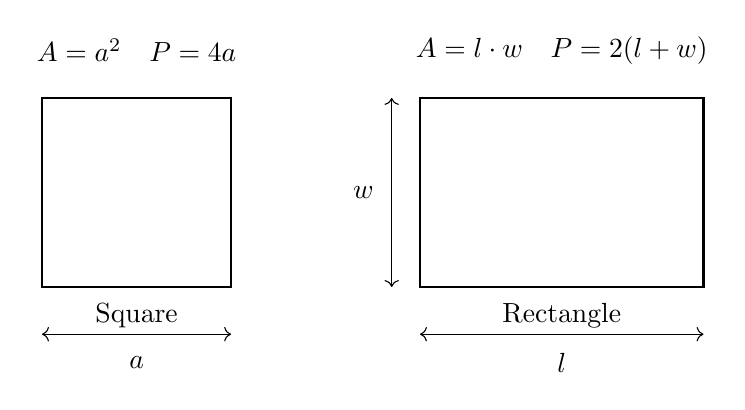
\begin{tikzpicture}[scale=1.2]
		% Square
		\draw[thick] (0,0) rectangle (2,2);
		\node at (1,-0.3) {Square};
		\draw[<->] (0,-0.5) -- (2,-0.5);
		\node at (1,-0.8) {\(a\)};
		\node at (1,2.5) {\(A = a^2 \quad P = 4a\)};

		% Rectangle
		\draw[thick] (4,0) rectangle (7,2);
		\node at (5.5,-0.3) {Rectangle};
		\draw[<->] (4,-0.5) -- (7,-0.5);
		\node at (5.5,-0.8) {\(l\)};
		\draw[<->] (3.7,0) -- (3.7,2);
		\node at (3.4,1) {\(w\)};
		\node at (5.5,2.5) {\(A = l \cdot w \quad P = 2(l+w)\)};
	\end{tikzpicture}
\end{center}

\subsection*{Circle and Triangle Types}
\begin{center}
	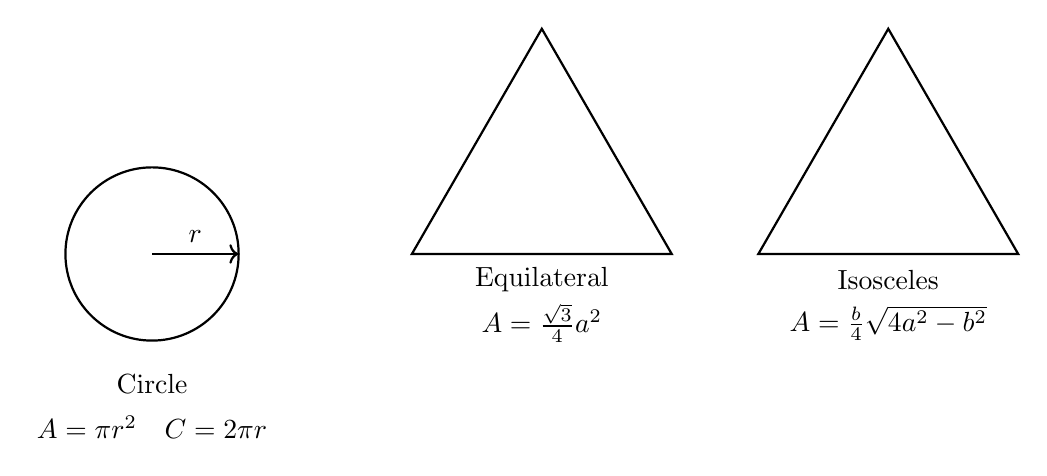
\begin{tikzpicture}[scale=1.1]
		% Circle
		\draw[thick] (0,0) circle(1cm);
		\draw[thick, ->] (0,0) -- (1,0);
		\node at (0.5,0.2) {\(r\)};
		\node at (0,-1.5) {Circle};
		\node at (0,-2) {\(A = \pi r^2 \quad C = 2\pi r\)};

		% Equilateral Triangle
		\draw[thick] (3,0) -- (4.5,2.6) -- (6,0) -- cycle;
		\node at (4.5,-0.3) {Equilateral};
		\node at (4.5,-0.8) {\(A = \frac{\sqrt{3}}{4} a^2\)};

		% Isosceles Triangle
		\draw[thick] (7,0) -- (8.5,2.6) -- (10,0) -- cycle;
		\node at (8.5,-0.3) {Isosceles};
		\node at (8.5,-0.8) {\(A = \frac{b}{4} \sqrt{4a^2 - b^2}\)};
	\end{tikzpicture}
\end{center}

\subsection*{Scalene Triangle, Trapezoid, Parallelogram}
\begin{center}
	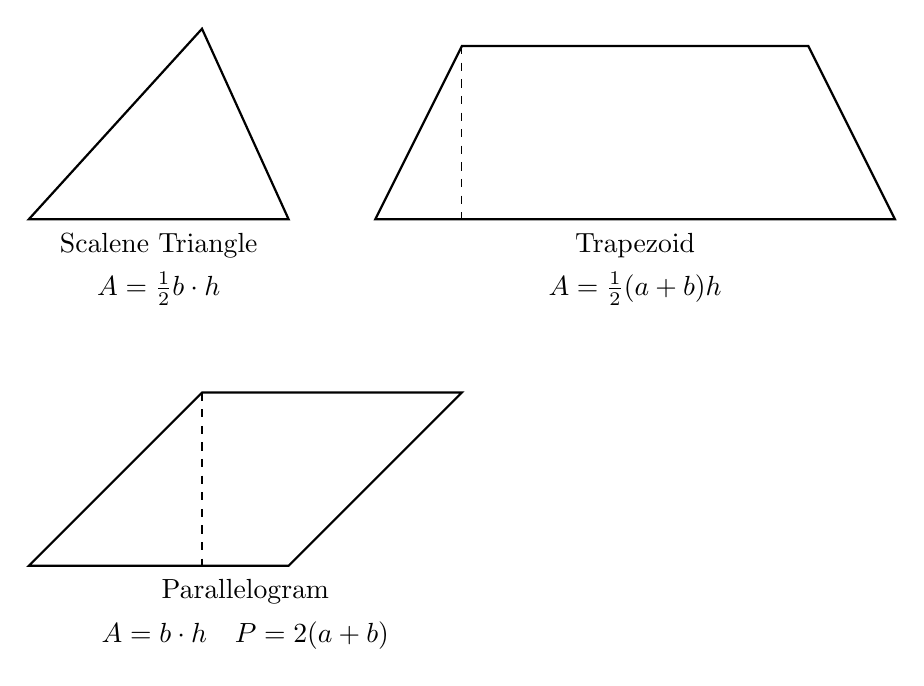
\begin{tikzpicture}[scale=1.1]
		% Scalene Triangle
		\draw[thick] (0,0) -- (2,2.2) -- (3,0) -- cycle;
		\node at (1.5,-0.3) {Scalene Triangle};
		\node at (1.5,-0.8) {\(A = \frac{1}{2} b \cdot h\)};

		% Trapezoid
		\draw[thick] (4,0) -- (5,2) -- (9,2) -- (10,0) -- cycle;
		\draw[dashed] (5,2) -- (5,0);
		\node at (7,-0.3) {Trapezoid};
		\node at (7,-0.8) {\(A = \frac{1}{2}(a+b)h\)};

		% Parallelogram
		\draw[thick] (0,-4) -- (2,-2) -- (5,-2) -- (3,-4) -- cycle;
		\draw[dashed] (2,-2) -- (2,-4);
		\node at (2.5,-4.3) {Parallelogram};
		\node at (2.5,-4.8) {\(A = b \cdot h \quad P = 2(a + b)\)};
	\end{tikzpicture}
\end{center}

\subsection{3D Geometric Figures with Formulas}

\subsubsection{Cube and Cylinder}
\begin{center}
	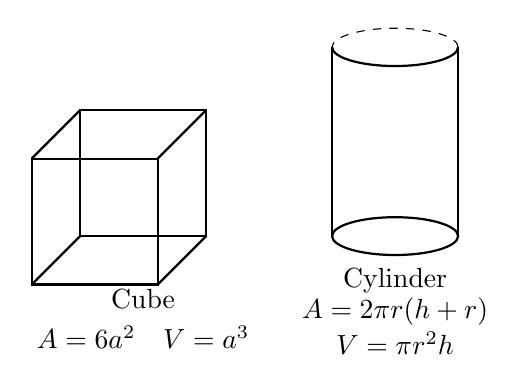
\begin{tikzpicture}[scale=0.8]
		% Cube
		\draw[thick] (0,0,0) -- (2,0,0) -- (2,2,0) -- (0,2,0) -- cycle;
		\draw[thick] (0,0,0) -- (0,0,2);
		\draw[thick] (2,0,0) -- (2,0,2);
		\draw[thick] (2,2,0) -- (2,2,2);
		\draw[thick] (0,2,0) -- (0,2,2);
		\draw[thick] (0,0,2) -- (2,0,2) -- (2,2,2) -- (0,2,2) -- cycle;
		\node at (1,-1) {Cube};
		\node at (1,-1.6) {\(A = 6a^2 \quad V = a^3\)};

		% Cylinder
		\begin{scope}[xshift=5cm]
			\draw[thick] (0,0) ellipse (1 and 0.3);
			\draw[thick] (-1,0) -- (-1,3);
			\draw[thick] (1,0) -- (1,3);
			\draw[thick] (-1,3) arc (180:360:1 and 0.3);
			\draw[dashed] (1,3) arc (0:180:1 and 0.3);
			\node at (0, -0.7) {Cylinder};
			\node at (0, -1.2) {\(A = 2\pi r(h + r)\)};
			\node at (0, -1.7) {\(V = \pi r^2 h\)};
		\end{scope}
	\end{tikzpicture}
\end{center}

\subsubsection{Cone and Sphere}
\begin{center}
	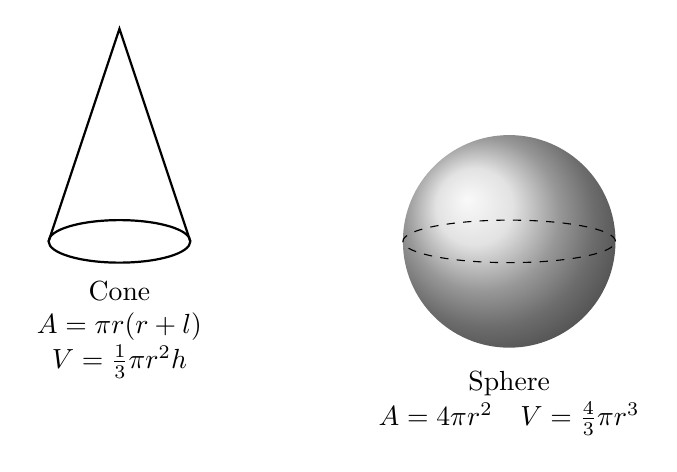
\begin{tikzpicture}[scale=0.9]
		% Cone
		\draw[thick] (0,0) ellipse (1 and 0.3);
		\draw[thick] (-1,0) -- (0,3) -- (1,0);
		\draw[dashed] (1,0) arc (0:180:1 and 0.3);
		\node at (0,-0.7) {Cone};
		\node at (0,-1.2) {\(A = \pi r(r + l)\)};
		\node at (0,-1.7) {\(V = \frac{1}{3} \pi r^2 h\)};

		% Sphere
		\begin{scope}[xshift=5.5cm]
			\shade[ball color=gray!30] (0,0) circle (1.5);
			\draw[dashed] (0,0) ellipse (1.5 and 0.3);
			\node at (0,-2) {Sphere};
			\node at (0,-2.5) {\(A = 4\pi r^2 \quad V = \frac{4}{3} \pi r^3\)};
		\end{scope}
	\end{tikzpicture}
\end{center}

\subsubsection{Pyramid and Prism}
\begin{center}
	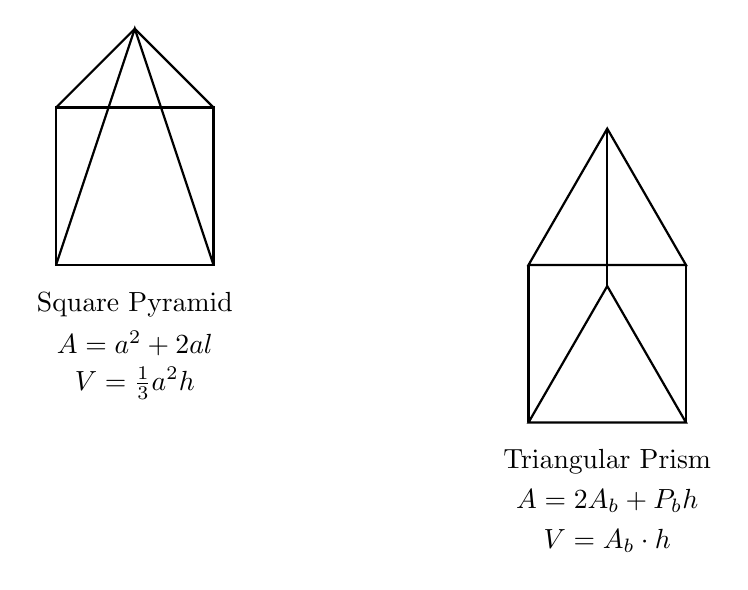
\begin{tikzpicture}[scale=1]
		% Square Pyramid
		\draw[thick] (0,0) -- (2,0) -- (2,2) -- (0,2) -- cycle;
		\draw[thick] (0,0) -- (1,3) -- (2,0);
		\draw[thick] (2,2) -- (1,3) -- (0,2);
		\node at (1,-0.5) {Square Pyramid};
		\node at (1,-1) {\(A = a^2 + 2al\)};
		\node at (1,-1.5) {\(V = \frac{1}{3}a^2 h\)};

		% Triangular Prism
		\begin{scope}[xshift=6cm]
			\draw[thick] (0,0) -- (2,0) -- (1,1.732) -- cycle;
			\draw[thick] (0,0) -- (0,-2);
			\draw[thick] (2,0) -- (2,-2);
			\draw[thick] (1,1.732) -- (1,-0.268);
			\draw[thick] (0,-2) -- (2,-2) -- (1,-0.268) -- cycle;
			\node at (1,-2.5) {Triangular Prism};
			\node at (1,-3) {\(A = 2A_b + P_b h\)};
			\node at (1,-3.5) {\(V = A_b \cdot h\)};
		\end{scope}
	\end{tikzpicture}
\end{center}

\subsection{Axioms of Euclidean Geometry}

Euclidean geometry is founded on a set of basic assumptions known as axioms or postulates, originally formulated by the Greek mathematician Euclid in his work \textit{Elements}. These axioms form the logical basis for plane geometry and include the following:

\begin{enumerate}[label=\Roman*.]
    \item \emph{Line Postulate:} A straight line segment can be drawn joining any two points.
    
    \item \emph{Extension Postulate:} Any straight line segment can be extended indefinitely in a straight line.
    
    \item \emph{Circle Postulate:} Given any straight line segment, a circle can be drawn having the segment as radius and one endpoint as center.
    
    \item \emph{Right Angle Postulate:} All right angles are congruent.
    
    \item \emph{Parallel Postulate:} If a line segment intersects two straight lines and makes the interior angles on the same side less than two right angles, then the two lines, if extended indefinitely, meet on that side.
\end{enumerate}

These five postulates define the framework of classical geometry in a flat (Euclidean) space. Notably, the fifth postulate—the parallel postulate—has been the subject of much scrutiny and led to the development of non-Euclidean geometries when it was altered or replaced.

\subsection{Types of Angles and Angle Relationships}

An angle is the distance between two rays or intercepting lines.

\begin{itemize}[label=\(-\)]
	\item If angle is less than \(90^\circ\) it is an \emph{acute} angle
	\item If it is exactly \(90^\circ\) it is a \emph{right} angle
	\item It is more than \(90^\circ\) but less than \(180^\circ\) it is called an \emph{obtuse} angle
\end{itemize}

Now lets look at other types of angles

\subsubsection{Vertical Angles}

When two lines intersect, they form two pairs of opposite (or vertical) angles. Vertical angles are always congruent. That is, if two angles are vertical, their measures are equal:
\[
\angle A = \angle B
\]
For example, if two lines intersect and form angles of \( 60^\circ \) and \( 120^\circ \), the angles opposite each other are both \( 60^\circ \) and both \( 120^\circ \).

\subsubsection{Adjacent Angles}

Adjacent angles are two angles that share a common side and a common vertex, and do not overlap. When two lines intersect, each pair of adjacent angles forms a straight angle (or a linear pair), summing to \(180^\circ\):
\[
\angle 1 + \angle 2 = 180^\circ
\]
This is known as the Linear Pair Postulate.

\subsubsection{Complementary Angles}

Complementary angles are two angles whose measures add up to \(90^\circ\):
\[
\angle X + \angle Y = 90^\circ
\]
Complementary angles do not have to be adjacent, but if two intersecting lines form a right angle, the two acute angles adjacent to the right angle may be complementary.

\subsubsection{Angles Generated by Traversals}

When a transversal crosses two or more lines, it forms several pairs of angles with specific relationships. Some key types include:

\begin{itemize}[label=\(-\)]
    \item \emph{Corresponding Angles:} Angles in the same relative position at each intersection. If the lines are parallel, corresponding angles are congruent:
    \[
    \angle 1 \cong \angle 2
    \]
    
    \item \emph{Alternate Interior Angles:} Angles that lie between the two lines but on opposite sides of the transversal. They are congruent if the lines are parallel:
    \[
    \angle 3 \cong \angle 4
    \]
    
    \item \emph{Alternate Exterior Angles:} Angles outside the two lines and on opposite sides of the transversal. Also congruent when the lines are parallel:
    \[
    \angle 5 \cong \angle 6
    \]
    
    \item \emph{Consecutive (Same-Side) Interior Angles:} Angles on the same side of the transversal and inside the parallel lines. These are supplementary:
    \[
    \angle 7 + \angle 8 = 180^\circ
    \]
\end{itemize}

\subsection{Triangle Similarity and Congruence}
Triangles can be compared using criteria of similarity or congruence, depending on whether their shapes are the same or both shape and size are identical.

\subsubsection{Triangle Congruence}
Two triangles are \emph{congruent} if all corresponding sides and angles are equal. This means the triangles are identical in shape and size. Common criteria for triangle congruence include:

\begin{itemize}[label=\(-\)]
    \item \emph{SSS (Side-Side-Side):} All three pairs of corresponding sides are equal.
    \item \emph{SAS (Side-Angle-Side):} Two pairs of sides and the angle between them are equal.
    \item \emph{ASA (Angle-Side-Angle):} Two pairs of angles and the included side are equal.
    \item \emph{AAS (Angle-Angle-Side):} Two angles and a non-included side are equal.
    \item \emph{HL (Hypotenuse-Leg):} For right triangles, if the hypotenuse and one leg are equal.
\end{itemize}

\subsubsection{Triangle Similarity}
Two triangles are \emph{similar} if their corresponding angles are equal and their corresponding sides are in proportion. This means they have the same shape but not necessarily the same size. Criteria for similarity include:

\begin{itemize}[label=\(-\)]
    \item \emph{AA (Angle-Angle):} Two pairs of corresponding angles are equal.
    \item \emph{SAS (Side-Angle-Side):} One pair of corresponding angles is equal, and the sides including those angles are in proportion.
    \item \emph{SSS (Side-Side-Side):} All three pairs of corresponding sides are in proportion.
\end{itemize}

\subsection{Visualizations of Triangle Similarity and Congruence}
\subsubsection{SSS (Side-Side-Side)}
A triangle is uniquely determined if all three sides are known.
\begin{center}
\begin{tikzpicture}[scale=1]
\draw[thick] (0,0) -- (5,0) node[midway, below] {\(c\)};
\draw[thick] (0,0) -- (2,3.5) node[midway, left] {\(b\)};
\draw[thick] (5,0) -- (2,3.5) node[midway, right] {\(a\)};
\node[below left] at (0,0) {\(A\)};
\node[below right] at (5,0) {\(B\)};
\node[above] at (2,3.5) {\(C\)};
\end{tikzpicture}
\end{center}

\subsubsection{SAS (Side-Angle-Side)}
A triangle is uniquely determined if two sides and the included angle are known.
\begin{center}
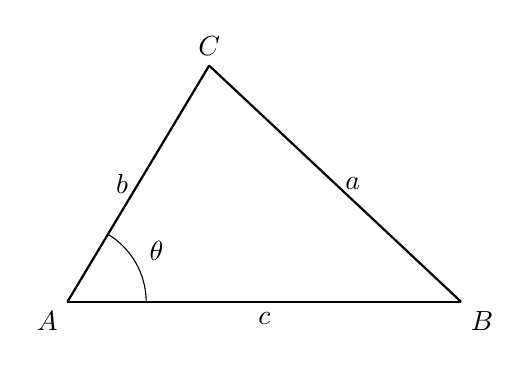
\begin{tikzpicture}[scale=1]
\coordinate (A) at (0,0);
\coordinate (B) at (5,0);
\coordinate (C) at (1.8,3);
\draw[thick] (A) -- (B) node[midway, below] {\(c\)};
\draw[thick] (A) -- (C) node[midway, left] {\(b\)};
\draw[thick] (B) -- (C) node[midway, right] {\(a\)};
\pic["\(\theta\)", draw=black, angle radius=1cm, angle eccentricity=1.3] {angle=B--A--C};
\node[below left] at (A) {\(A\)};
\node[below right] at (B) {\(B\)};
\node[above] at (C) {\(C\)};
\end{tikzpicture}
\end{center}

\subsubsection{ASA (Angle-Side-Angle)}
A triangle is uniquely determined if two angles and the included side are known.
\begin{center}
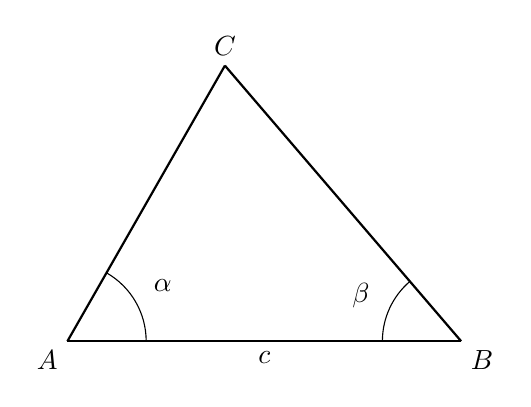
\begin{tikzpicture}[scale=1]
\coordinate (A) at (0,0);
\coordinate (B) at (5,0);
\coordinate (C) at (2,3.5);
\draw[thick] (A) -- (B) node[midway, below] {\(c\)};
\draw[thick] (A) -- (C);
\draw[thick] (B) -- (C);
\pic["\(\alpha\)", draw=black, angle radius=1cm, angle eccentricity=1.4] {angle=B--A--C};
\pic["\(\beta\)", draw=black, angle radius=1cm, angle eccentricity=1.4] {angle=C--B--A};
\node[below left] at (A) {\(A\)};
\node[below right] at (B) {\(B\)};
\node[above] at (C) {\(C\)};
\end{tikzpicture}
\end{center}

\subsubsection{AAS (Angle-Angle-Side)}
A triangle is uniquely determined if two angles and a non-included side are known.
\begin{center}
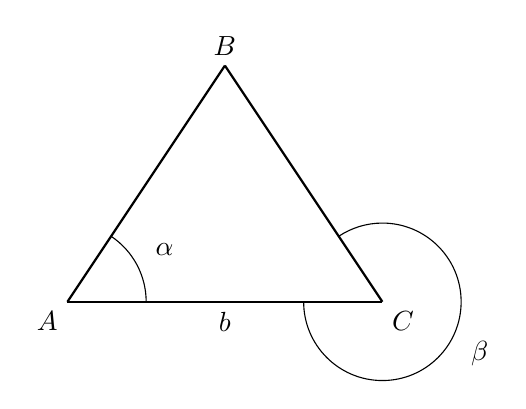
\begin{tikzpicture}[scale=1]
\coordinate (A) at (0,0);
\coordinate (C) at (4,0);
\coordinate (B) at (2,3);
\draw[thick] (A) -- (C) node[midway, below] {\(b\)};
\draw[thick] (A) -- (B);
\draw[thick] (B) -- (C);
\pic["\(\alpha\)", draw=black, angle radius=1cm, angle eccentricity=1.4] {angle=C--A--B};
\pic["\(\beta\)", draw=black, angle radius=1cm, angle eccentricity=1.4] {angle=A--C--B};
\node[below left] at (A) {\(A\)};
\node[below right] at (C) {\(C\)};
\node[above] at (B) {\(B\)};
\end{tikzpicture}
\end{center}

\subsubsection{SSA (Side-Side-Angle)}
Two sides and a non-included angle do \emph{not always} determine a unique triangle. This case is ambiguous and can result in:
\begin{itemize}
    \item One triangle (when the opposite side is long enough),
    \item Two triangles (ambiguous case),
    \item No triangle (when the side is too short).
\end{itemize}
\begin{center}
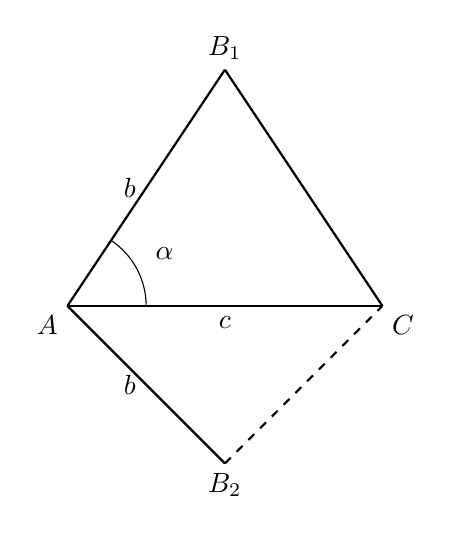
\begin{tikzpicture}[scale=1]
\coordinate (A) at (0,0);
\coordinate (C) at (4,0);
\coordinate (B1) at (2,3); % triangle 1
\coordinate (B2) at (2,-2); % triangle 2
\draw[thick] (A) -- (C) node[midway, below] {\(c\)};
\draw[thick] (A) -- (B1) node[midway, left] {\(b\)};
\draw[thick] (A) -- (B2) node[midway, left] {\(b\)};
\draw[thick, dashed] (B2) -- (C);
\draw[thick] (B1) -- (C);
\pic["\(\alpha\)", draw=black, angle radius=1cm, angle eccentricity=1.4] {angle=C--A--B1};
\node[below left] at (A) {\(A\)};
\node[below right] at (C) {\(C\)};
\node[above] at (B1) {\(B_1\)};
\node[below] at (B2) {\(B_2\)};
\end{tikzpicture}
\end{center}

\subsection{Triangle Medians, Angle Bisectors, and Altitudes}

In any triangle, there are special line segments that connect vertices to specific points on the opposite sides. These segments play key roles in triangle geometry and have unique properties.

\subsubsection*{Median}

A \emph{median} of a triangle is a line segment that connects a vertex to the midpoint of the opposite side. Every triangle has three medians, and they intersect at a single point called the \emph{centroid}, which is the triangle’s center of mass. The centroid divides each median in a ratio of \( 2:1 \), with the longer part closer to the vertex.

\subsubsection*{Angle Bisector}

An \emph{angle bisector} is a line segment that divides an angle of the triangle into two equal parts and extends to the opposite side. All three angle bisectors intersect at a point called the \emph{incenter}, which is the center of the triangle's incircle (the largest circle that fits inside the triangle and touches all three sides).

\subsubsection*{Altitude}

An \emph{altitude} of a triangle is a perpendicular segment from a vertex to the line containing the opposite side (not necessarily within the triangle). Altitudes intersect at a point called the \emph{orthocenter}. Unlike medians and bisectors, altitudes can fall outside the triangle in obtuse triangles.

\[
\text{Centroid} \rightarrow \text{Intersection of medians}\]
\[
\text{Incenter} \rightarrow \text{Intersection of angle bisectors}\]
\[
\text{Orthocenter} \rightarrow \text{Intersection of altitudes}
\]

\subsection{The Midsegment Theorem}

The \emph{Midsegment Theorem} states that the segment connecting the midpoints of two sides of a triangle is:

\begin{itemize}[label=\(-\)]
    \item \emph{Parallel} to the third side of the triangle
    \item \emph{Half the length} of the third side
\end{itemize}

Let \( \triangle ABC \) be a triangle, and let \( D \) and \( E \) be the 
midpoints of sides \( AB \) and \( AC \), respectively. Then the segment \( \overline{DE} \) is 
the \emph{midsegment}, and we have:
\[
\overline{DE} \parallel \overline{BC} \quad \text{and} \quad DE = \frac{1}{2} BC
\]

This theorem is useful in coordinate geometry, triangle proofs, 
and for simplifying complex geometric relationships within triangles.

\subsection{Intercept Theorems}

The intercept theorems describe relationships between segment lengths when two rays from a point intersect two parallel lines. They are based on similar triangles and allow us to calculate unknown lengths using proportions.

\subsubsection{First Intercept Theorem}

If two rays start from a common point and are intersected by two parallel lines, then:

\[
	\frac{a}{a'} = \frac{b}{b'}
\]

where \(a\) and \(b\) are segments on one ray, and \(a'\), \(b'\) are the corresponding segments on the other ray.

\begin{center}
	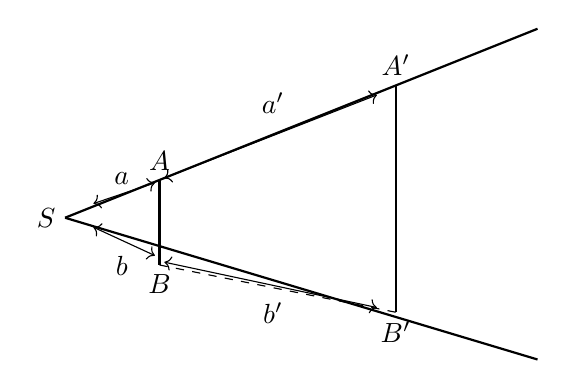
\begin{tikzpicture}[scale=1.2]
		% Rays
		\draw[thick] (0,0) -- (5,2); % upper ray
		\draw[thick] (0,0) -- (5,-1.5); % lower ray

		% Parallels
		\draw[thick] (1,0.4) -- (1,-0.5);
		\draw[thick] (3.5,1.4) -- (3.5,-1);

		% Points
		\node at (-0.2,0) {\(S\)};
		\node[above] at (1,0.4) {\(A\)};
		\node[below] at (1,-0.5) {\(B\)};
		\node[above] at (3.5,1.4) {\(A'\)};
		\node[below] at (3.5,-1) {\(B'\)};

		% Helper lines
		\draw[dashed] (1,0.4) -- (3.5,1.4);
		\draw[dashed] (1,-0.5) -- (3.5,-1);

		% Length labels
		\draw[<->] (0.3,0.15) -- (0.95,0.37);
		\node[above] at (0.6,0.25) {\(a\)};
		\draw[<->] (1.05,0.42) -- (3.3,1.3);
		\node[above] at (2.2,1) {\(a'\)};

		\draw[<->] (0.3,-0.1) -- (0.95,-0.4);
		\node[below] at (0.6,-0.3) {\(b\)};
		\draw[<->] (1.05,-0.47) -- (3.3,-0.95);
		\node[below] at (2.2,-0.8) {\(b'\)};
	\end{tikzpicture}
\end{center}

\subsubsection{Second Intercept Theorem (General Form)}

If a ray intersects two parallel lines, the segments from the origin point to the lines are in the same ratio as the segments along the parallels:

\[
	\frac{SA}{SA'} = \frac{SB}{SB'} \quad \text{and} \quad \frac{AB}{A'B'} = \frac{SA}{SA'}
\]

\begin{center}
	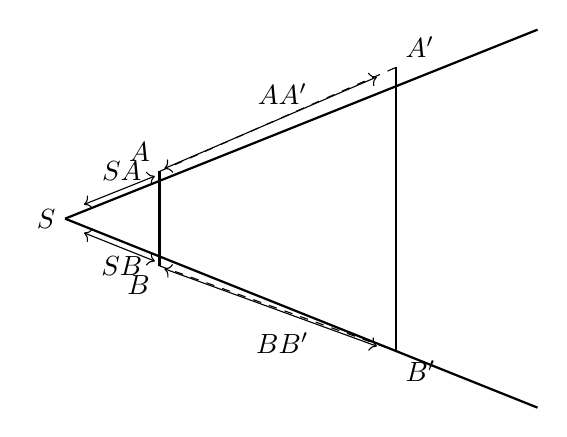
\begin{tikzpicture}[scale=1.2]
		% Rays
		\draw[thick] (0,0) -- (5,2); % upper ray
		\draw[thick] (0,0) -- (5,-2); % lower ray

		% Parallels
		\draw[thick] (1,0.5) -- (1,-0.5);
		\draw[thick] (3.5,1.6) -- (3.5,-1.4);

		% Points
		\node at (-0.2,0) {\(S\)};
		\node[above left] at (1,0.5) {\(A\)};
		\node[below left] at (1,-0.5) {\(B\)};
		\node[above right] at (3.5,1.6) {\(A'\)};
		\node[below right] at (3.5,-1.4) {\(B'\)};

		% Helper lines
		\draw[dashed] (1,0.5) -- (3.5,1.6);
		\draw[dashed] (1,-0.5) -- (3.5,-1.4);
		\draw[dashed] (1,0.5) -- (1,-0.5);
		\draw[dashed] (3.5,1.6) -- (3.5,-1.4);

		% Length labels
		\draw[<->] (0.2,0.15) -- (0.95,0.45);
		\node[above] at (0.6,0.3) {\(SA\)};
		\draw[<->] (1.05,0.53) -- (3.3,1.5);
		\node[above] at (2.3,1.1) {\(AA'\)};

		\draw[<->] (0.2,-0.15) -- (0.95,-0.45);
		\node[below] at (0.6,-0.3) {\(SB\)};
		\draw[<->] (1.05,-0.53) -- (3.3,-1.35);
		\node[below] at (2.3,-1.1) {\(BB'\)};
	\end{tikzpicture}
\end{center}

\subsection{Proof of the Pythagorean Theorem}

We want to prove that \(c^2 = a^2 + b^2\) is a true statement.
\vspace{\baselineskip}

Lets a build a Square with area \(c^2\) and take our original triangle and put it on the sides
on the square.
\vspace{\baselineskip}

This will create a square of sides \((a+b)^2\) which is bigger than the inner square \(c^2\).
\vspace{\baselineskip}

Now lets find the area \(c^2\) using what we known about this shape.

\begin{align*}
	{(a + b)}^2 = 4(\frac{ab}{2}) + c^2\\
	{(a + b)}^2 = 2ab + c^2\\
	a^2 + 2ab + b^2 = 2ab + c^2\\
	a^2 + b^2 = c^2
\end{align*}

\QED



\section{Trigonometry}
In this section, we will cover a variety of trigonometric functions and their properties.

\subsection{Trigonometric Functions}
\begin{itemize}[label=\(-\)]
    \item \( \sin(x) = \frac{1}{\csc(x)} \)
    \item \( \cos(x) = \frac{1}{\sec(x)}\)
    \item \( \tan(x) = \frac{\sin(x)}{\cos(x)}\ = \frac{1}{\cot(x)}\)
    \item \( \csc(x) = \frac{1}{\sin(x)} \)
    \item \( \sec(x) = \frac{1}{\cos(x)} \)
    \item \( \cot(x) = \frac{\cos(x)}{\sin(x)} = \frac{1}{\tan(x)} \)
\end{itemize}

\subsection{SOH-CAH-TOA}
\begin{itemize}[label=\(-\)]
    \item \( \sin(x) = \frac{\text{opposite}}{\text{hypotenuse}} \)
    \item \( \cos(x) = \frac{\text{adjacent}}{\text{hypotenuse}} \)
    \item \( \tan(x) = \frac{\text{opposite}}{\text{adjacent}} \)
\end{itemize}

\subsection{Pythagorean Identities}
\begin{itemize}[label=\(-\)]
    \item \( \sin^2(x) + \cos^2(x) = 1 \)
    \item \( 1 + \tan^2(x) = \sec^2(x) \)
    \item \( 1 + \cot^2(x) = \csc^2(x) \)
\end{itemize}

\subsection{Sum and Difference Formulas}
\begin{itemize}[label=\(-\)]
    \item \( \sin(a + b) = \sin(a)\cos(b) + \cos(a)\sin(b) \)
    \item \( \sin(a - b) = \sin(a)\cos(b) - \cos(a)\sin(b) \)
    \item \( \cos(a + b) = \cos(a)\cos(b) - \sin(a)\sin(b) \)
    \item \( \cos(a - b) = \cos(a)\cos(b) + \sin(a)\sin(b) \)
    \item \( \tan(a + b) = \frac{\tan(a) + \tan(b)}{1 - \tan(a)\tan(b)}\)
    \item \( \tan(a - b) = \frac{\tan(a) - \tan(b)}{1 + \tan(a)\tan(b)}\)
\end{itemize}

\begin{center}
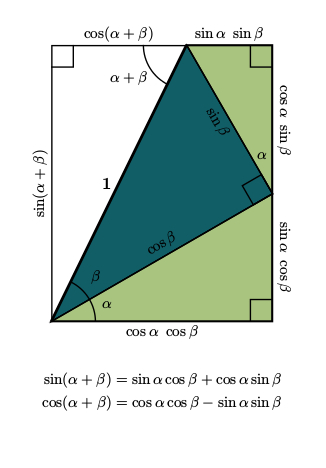
\includegraphics{trig.jpg}
\end{center}

\subsection{Double Angle Formulas}
\begin{itemize}[label=\(-\)]
    \item \( \sin(2x) = 2\sin(x)\cos(x) \)
    \item \( \cos(2x) = \cos^2(x) - \sin^2(x) = 2\cos^2(x) - 1 = 1 - 2\sin^2(x) \)
    \item \( \tan(2x) = \frac{2\tan(x)}{1 - \tan^2(x)}\)
    \item \( \csc(2x) = \frac{2\csc(x)\sec(x)}{1 - \tan^2(x)}\)
    \item \( \sec(2x) = \frac{1 + \tan^2(x)}{2\tan(x)}\)
    \item \( \cot(2x) = \frac{1 - \tan^2(x)}{2\tan(x)}\)
\end{itemize}

\subsection{Half Angle Formulas}
\begin{itemize}[label=\(-\)]
    \item \( \sin\left(\frac{x}{2}\right) = \pm\sqrt{\frac{1 - \cos(x)}{2}} \)
    \item \( \cos\left(\frac{x}{2}\right) = \pm\sqrt{\frac{1 + \cos(x)}{2}} \)
    \item \( \tan\left(\frac{x}{2}\right) = \frac{\sin(x)}{1 + \cos(x)} = \frac{1 - \cos(x)}{\sin(x)} = \frac{\tan(x)}{1 + \tan^2(x)}\)
    \item \( \csc\left(\frac{x}{2}\right) = \frac{1}{\sin\left(\frac{x}{2}\right)} = \pm\sqrt{\frac{2}{1 - \cos(x)}} \)
    \item \( \sec\left(\frac{x}{2}\right) = \frac{1}{\cos\left(\frac{x}{2}\right)} = \pm\sqrt{\frac{2}{1 + \cos(x)}} \)
    \item \( \cot\left(\frac{x}{2}\right) = \frac{1}{\tan\left(\frac{x}{2}\right)} = \frac{1 + \cos(x)}{\sin(x)} = \frac{1 - \tan^2(x)}{2\tan(x)}\)
\end{itemize}

\subsection{Product to Sum Formulas}
\begin{itemize}[label=\(-\)]
    \item \( \sin(a)\sin(b) = \frac{1}{2}[\cos(a - b) - \cos(a + b)] \)
    \item \( \cos(a)\cos(b) = \frac{1}{2}[\cos(a - b) + \cos(a + b)] \)
    \item \( \sin(a)\cos(b) = \frac{1}{2}[\sin(a + b) + \sin(a - b)] \)
    \item \( \cos(a)\sin(b) = \frac{1}{2}[\sin(a + b) - \sin(a - b)] \)
\end{itemize}

\subsection{Power Reducing Formulas}
\begin{itemize}[label=\(-\)]
    \item \( \sin^2(x) = \frac{1 - \cos(2x)}{2} \)
    \item \( \cos^2(x) = \frac{1 + \cos(2x)}{2} \)
    \item \( \tan^2(x) = \frac{1 - \cos(2x)}{1 + \cos(2x)}\)
    \item \( \csc^2(x) = \frac{1}{\sin^2(x)} = \frac{2}{1 - \cos(2x)} \)
    \item \( \sec^2(x) = \frac{1}{\cos^2(x)} = \frac{2}{1 + \cos(2x)} \)
    \item \( \cot^2(x) = \frac{1}{\tan^2(x)} = \frac{1 + \cos(2x)}{1 - \cos(2x)}\)
\end{itemize}

\subsection{Even and Odd Functions}
\begin{itemize}[label=\(-\)]
    \item \( \sin(-x) = -\sin(x) \)
    \item \( \cos(-x) = \cos(x) \)
    \item \( \tan(-x) = -\tan(x) \)
    \item \( \csc(-x) = -\csc(x) \)
    \item \( \sec(-x) = \sec(x) \)
    \item \( \cot(-x) = -\cot(x) \)
\end{itemize}

\subsection{Graph Identity}
\(\cos(x) = \sin(x + \frac{\pi}{2})\)

\subsection{Trigonometric Values}
\smallskip
\begin{center}
    \renewcommand{\arraystretch}{1.4}
    \begin{tabular}{|c|c|c|c|}
    \hline
    \(\theta\) (radians) & \(\sin(\theta)\) & \(\cos(\theta)\) & \(\tan(\theta)\) \\
    \hline
    \(0\) & \(0\) & \(1\) & \(0\) \\
    \hline
    \(\frac{\pi}{6}\) & \(\frac{1}{2}\) & \(\frac{\sqrt{3}}{2}\) & \(\frac{1}{\sqrt{3}}\) \\
    \hline
    \(\frac{\pi}{4}\) & \(\frac{\sqrt{2}}{2}\) & \(\frac{\sqrt{2}}{2}\) & \(1\) \\
    \hline
    \(\frac{\pi}{3}\) & \(\frac{\sqrt{3}}{2}\) & \(\frac{1}{2}\) & \(\sqrt{3}\) \\
    \hline
    \(\frac{\pi}{2}\) & \(1\) & \(0\) & undefined \\
    \hline
    \(\frac{2\pi}{3}\) & \(\frac{\sqrt{3}}{2}\) & \(-\frac{1}{2}\) & \(-\sqrt{3}\) \\
    \hline
    \(\frac{3\pi}{4}\) & \(\frac{\sqrt{2}}{2}\) & \(-\frac{\sqrt{2}}{2}\) & \(-1\) \\
    \hline
    \(\frac{5\pi}{6}\) & \(\frac{1}{2}\) & \(-\frac{\sqrt{3}}{2}\) & \(-\frac{1}{\sqrt{3}}\) \\
    \hline
    \(\pi\) & \(0\) & \(-1\) & \(0\) \\
    \hline
    \(\frac{7\pi}{6}\) & \(-\frac{1}{2}\) & \(-\frac{\sqrt{3}}{2}\) & \(\frac{1}{\sqrt{3}}\) \\
    \hline
    \(\frac{5\pi}{4}\) & \(-\frac{\sqrt{2}}{2}\) & \(-\frac{\sqrt{2}}{2}\) & \(1\) \\
    \hline
    \(\frac{4\pi}{3}\) & \(-\frac{\sqrt{3}}{2}\) & \(-\frac{1}{2}\) & \(\sqrt{3}\) \\
    \hline
    \(\frac{3\pi}{2}\) & \(-1\) & \(0\) & undefined \\
    \hline
    \(\frac{5\pi}{3}\) & \(-\frac{\sqrt{3}}{2}\) & \(\frac{1}{2}\) & \(-\sqrt{3}\) \\
    \hline
    \(\frac{7\pi}{4}\) & \(-\frac{\sqrt{2}}{2}\) & \(\frac{\sqrt{2}}{2}\) & \(-1\) \\
    \hline
    \(\frac{11\pi}{6}\) & \(-\frac{1}{2}\) & \(\frac{\sqrt{3}}{2}\) & \(-\frac{1}{\sqrt{3}}\) \\
    \hline
    \(2\pi\) & \(0\) & \(1\) & \(0\) \\
    \hline
    \end{tabular}
\end{center}

\subsection{Unit Circle and Trigonometric Functions}

The unit circle is a circle with a radius of 1 centered at the origin. Trigonometric functions like \(\sin(\theta)\), \(\cos(\theta)\), and \(\tan(\theta)\) can be defined based on the coordinates of a point on the circle corresponding to angle \(\theta\).

\begin{center}
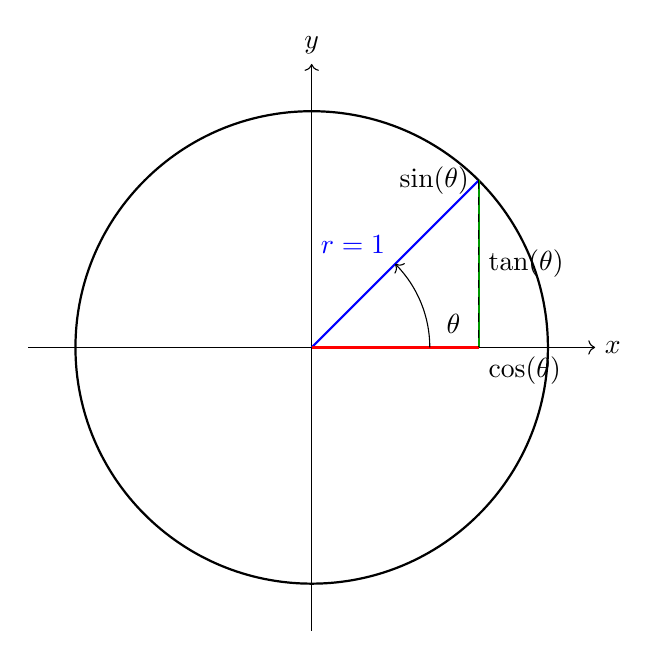
\begin{tikzpicture}[scale=3]
    % Draw unit circle
    \draw[thick] (0,0) circle (1);
    
    % Axes
    \draw[->] (-1.2,0) -- (1.2,0) node[right] {\(x\)};
    \draw[->] (0,-1.2) -- (0,1.2) node[above] {\(y\)};
    
    % Angle and triangle
    \draw[thick, blue] (0,0) -- ({cos(45)},{sin(45)}) node[pos=0.5, above left] {\(r=1\)};
    \draw[thick, red] (0,0) -- ({cos(45)},0);
    \draw[thick, green!60!black] ({cos(45)},0) -- ({cos(45)},{sin(45)});
    
    % Dotted lines
    \draw[dashed] ({cos(45)},{sin(45)}) -- ({cos(45)},0);
    
    % Angle arc
    \draw[->] (0.5,0) arc[start angle=0,end angle=45,radius=0.5];
    \node at (0.6,0.1) {\(\theta\)};
    
    % Labels
    \node[below right] at ({cos(45)},0) {\(\cos(\theta)\)};
    \node[left] at ({cos(45)},{sin(45)}) {\(\sin(\theta)\)};
    \node[right] at ({cos(45)}, {sin(45)/2}) {\(\tan(\theta)\)};
\end{tikzpicture}
\end{center}

\subsection{Definitions on the Unit Circle:}
\begin{itemize}[label=\(-\)]
    \item \(\cos(\theta)\) is the \emph{x-coordinate} of the point on the circle.
    \item \(\sin(\theta)\) is the \emph{y-coordinate}.
    \item \(\tan(\theta) = \dfrac{\sin(\theta)}{\cos(\theta)}\) is the ratio of the opposite side to the adjacent side in the triangle.
\end{itemize}


\subsection{Trigonometric Rules}

\begin{itemize}[label =\(-\)]
	\item \(\frac{\sin \alpha}{a} = \frac{\sin \beta}{b} = \frac{\sin \gamma}{c}\)
	\item \(c^2 = a^2 + b^2 - 2ab \cos \gamma\)
	\item \(\frac{a - b}{a + b} = \frac{\tan \frac{1}{2}(\alpha - \beta)}{\tan \frac{1}{2} (\alpha + \beta)}\)
\end{itemize}

\subsection{Proof of the Cosine Rule}

The \emph{Cosine Rule} relates the lengths of the sides of a triangle to the cosine of one of its angles. For any triangle \( ABC \) with sides \( a = BC \), \( b = AC \), and \( c = AB \), and angle \( \gamma = \angle ACB \), the cosine rule states:

\[
c^2 = a^2 + b^2 - 2ab\cos(\gamma)
\]

\textbf{Proof}

Consider triangle \( ABC \), and place it on the coordinate plane such that point \( C \) is at the origin \( (0,0) \), point \( B \) is at \( (a,0) \), and point \( A \) 
lies somewhere in the plane. Let angle \( \gamma = \angle ACB \).
\\\\
Let the coordinates of point \( A \) be \( (b\cos\gamma, b\sin\gamma) \), since \( b = AC \) and we’re using polar coordinates to define its location relative to point \( C \).
\\\\
Using the distance formula to find side \( c = AB \), we get:

\begin{align*}
c^2 &= (a - b\cos\gamma)^2 + (0 - b\sin\gamma)^2 \\
&= a^2 - 2ab\cos\gamma + b^2\cos^2\gamma + b^2\sin^2\gamma \\
&= a^2 + b^2(\cos^2\gamma + \sin^2\gamma) - 2ab\cos\gamma \\
&= a^2 + b^2 - 2ab\cos\gamma
\end{align*}

since \( \cos^2\gamma + \sin^2\gamma = 1 \).
\\\\
Thus, we have proven that:

\[
c^2 = a^2 + b^2 - 2ab\cos\gamma
\]

\QED
\newpage

\newpage
\section{Linear Systems of Equations}

In this section, we will discuss the solution of linear systems of equations. A linear system of 
equations is a set of equations that can be expressed in the form:

\begin{align*}
	a_{11}x_1 + a_{12}x_2 + \cdots + a_{1n}x_n & = b_1  \\
	a_{21}x_1 + a_{22}x_2 + \cdots + a_{2n}x_n & = b_2  \\
	& \vdots \\
	a_{m1}x_1 + a_{m2}x_2 + \cdots + a_{mn}x_n & = b_m,
\end{align*}

where \( a_{ij} \) are the coefficients of the variables \( x_j \), and \( b_i \) are the constants 
on the right-hand side of the equations. The goal is to find the values of \( x_1, x_2, \ldots, x_n \) 
that satisfy all equations simultaneously.

\subsection{Matrix Representation}

A linear system can be represented in matrix form as:

\[
	A x = b
\]

Where \( A \) is the coefficient matrix, \( x \) is the vector of variables, and \( b \) is the vector 
of constants. The coefficient matrix \( A \) is an \( m \times n \) matrix, where \( m \) is the number 
of equations and \( n \) is the number of variables. The vector \( x \) is an \( n \times 1 \) column 
vector, and the vector \( b \) is an \( m \times 1 \) column vector. 


\subsection{Solution Set of a Linear System}

In the context of Definition 6.1, the solution set \( L(A, b) \) of the system of equations associated 
with \( (A, b) \) is defined as

\[
	L(A, b) := \{ x \in K^n \mid Ax = b \}.
\]

\subsection{Equality of the Rank \texorpdfstring{\(\operatorname{rg}(A) = \operatorname{rg}_S(A)\)}{}}

We have \(\operatorname{rg}(A) = \operatorname{rg}_S(A)\).
\vspace{\baselineskip}

\textbf{Proof:} 

For \(x = {(x_1, \ldots, x_n)}^T \in K^n\), it holds that

\[
	Ax = \sum_{i=1}^{n} x_i a_i.
\]

It follows that

\[
	\operatorname{rg}(A) = \operatorname{rg}(L_A) = \dim(\operatorname{Im}(L_A))
	= \dim\left(\{L_A(x) \mid x \in K^n\}\right)
	= \dim\left(\{Ax \mid x \in K^n\}\right)
\]

\[
	= \dim\left\{ \sum_{i=1}^{n} x_i a_i \,\middle|\, x_i \in K \right\}
	= \dim(L(a_1, \ldots, a_n)) = \operatorname{rg}_S(A).
\]

\subsection{Solvability of the Linear System \texorpdfstring{\(Ax = b\)}{}}

The linear system \(Ax = b\) is solvable if and only if

\[
	\operatorname{rg}(a_1, \ldots, a_n) = \operatorname{rg}(a_1, \ldots, a_n, b).
\]

More concisely, we write

\[
	\operatorname{rg}(A) = \operatorname{rg}(A, b).
\]

\textbf{Proof:} 

We have

\[
	Ax = (a_1, \ldots, a_n)x = x_1 a_1 + \cdots + x_n a_n = b.
\]

Therefore, a solution vector \(x\) exists if and only if

\[
	b \in L(a_1, \ldots, a_n) \quad \Leftrightarrow \quad \operatorname{rg}(A) = \operatorname{rg}(A, b),
\]

where \(L(a_1, \ldots, a_n)\) denotes the linear span of \(a_1, \ldots, a_n\).

\subsection{Solution Set of the Linear System \texorpdfstring{\(Ax = b\)}{}}

Let \(x_s \in K^n\) be a solution of \(Ax = b\). Then the solution set is given by

\[
	L(A, b) = x_s + \ker(A) = \{x_s + x \mid x \in \ker(A)\}.
\]

\textbf{Proof:}

\[
	x \in \ker(A) \;\Leftrightarrow\; Ax = 0 \;\Leftrightarrow\; A(x_s + x) = Ax_s + Ax = Ax_s = b.
\]


\subsection{Gaussian Elimination}

Gaussian elimination is a method for solving linear systems by transforming the system into an upper 
triangular form. The steps involved in Gaussian elimination are:

\begin{enumerate}
	\item Forward elimination: Transform the system into an upper triangular form by eliminating the 
	      variables from the equations.
	\item Back substitution: Solve for the variables starting from the last equation and substituting 
	      back into the previous equations.
\end{enumerate}

The forward elimination process involves performing row operations on the augmented matrix 
\([A | \mathbf{b}]\) to create zeros below the diagonal. The row operations include:

\begin{itemize}
	\item Swapping two rows
	\item Multiplying a row by a non-zero scalar
	\item Adding or subtracting a multiple of one row from another row
\end{itemize}

Once the matrix is in upper triangular form, back substitution is used to find the values of the 
variables. The last equation gives the value of the last variable, which can then be substituted into 
the previous equations to find the other variables.

\subsection{Gauss-Jordan Elimination}

Gauss-Jordan elimination is an extension of Gaussian elimination that transforms the matrix into 
reduced row echelon form (RREF). In RREF, each leading entry in a row is 1, and all entries above and 
below the leading entry are zeros. The steps involved in Gauss-Jordan elimination are:

\begin{enumerate}
	\item Forward elimination: Transform the system into an upper triangular form.
	\item Back substitution: Transform the upper triangular matrix into RREF by eliminating the entries 
		  above the leading 1s.
	\item Solve for the variables directly from the RREF matrix.
\end{enumerate}

The Gauss-Jordan elimination method is particularly useful for finding the inverse of a matrix, as it 7
can be applied to the augmented matrix \([A | I]\), where \(I\) is the identity matrix. If the left side 
of the augmented matrix becomes \(I\), then the right side will be the inverse of \(A\).
\vspace{\baselineskip}

\textbf{Example:}
\vspace{\baselineskip}

Solve the following system of equations using Gaussian elimination:

\begin{align*}
	2x + 3y + z  & = 1 \\
	4x + y - z   & = 2 \\
	-2x + y + 3z & = 3
\end{align*}

\textbf{Solution:} The augmented matrix for the system is:

\[
	\begin{pmatrix}
		2  & 3 & 1  & | & 1 \\
		4  & 1 & -1 & | & 2 \\
		-2 & 1 & 3  & | & 3
	\end{pmatrix}
\]

Performing row operations to eliminate the variables, we can transform the matrix into upper triangular form:

\[
	\begin{pmatrix}
		1 & \frac{3}{2} & \frac{1}{2} & | & \frac{1}{2} \\
		0 & -5          & -3          & | & 0           \\
		0 & 0           & 1           & | & 1
	\end{pmatrix}
\]

Now, we can perform back substitution to find the values of \(x\), \(y\), and \(z\):

\begin{align*}
	z           & = 1                           \\
	-5y - 3z    & = 0 \implies y = -\frac{3}{5} \\
	2x + 3y + z & = 1 \implies x = \frac{1}{5}
\end{align*}

Thus, the solution to the system is:

\begin{align*}
	x & = \frac{1}{5}  \\
	y & = -\frac{3}{5} \\
	z & = 1
\end{align*}

\subsection{Homogeneous Linear Equations}

A linear equation is said to be \emph{homogeneous} if its constant term is zero. That is, it 
can be written in the form:

\[
	a_1 x_1 + a_2 x_2 + \cdots + a_n x_n = 0
\]

Such equations always have at least the trivial solution \(x_1 = x_2 = \cdots = x_n = 0\).

\subsection{Particular Solution}

A particular solution to a linear system of equations is a specific solution that satisfies the system. 
It can be found using various methods, including substitution, elimination, or matrix methods. A 
particular solution is not unique; there may be multiple particular solutions depending on the system.
A particular solution can be found by substituting specific values for the variables and solving for the 
remaining variables. For example, in the system

\begin{align*}
	2x + 3y & = 5 \\
	4x - y  & = 1
\end{align*}

we can substitute \(x = 1\) into the first equation to find \(y\):

\begin{align*}
	2(1) + 3y & = 5 \\
	3y        & = 3 \\
	y         & = 1
\end{align*}

Thus, \((x, y) = (1, 1)\) is a particular solution to the system. However, this is not the only solution; 
other values of \(x\) may yield different values of \(y\).

\subsection{General = Particular + Homogeneous}

The general solution of a linear system of equations is the complete set of solutions that satisfy the 
system. It can be expressed as the sum of a particular solution and the general solution of the associated 
homogeneous system.

The general solution can be written as:

\[
	x = x_p + x_h
\]

Where \( x_p \) is a particular solution to the non-homogeneous system, and \( x_h \) is the general 
solution to the homogeneous system. The homogeneous system is obtained by setting the right-hand side 
of the equations to zero:

\[
	A x = 0
\]

The theorem says:

Any linear system's solution set has the form:

\[
	\left\{ \vec{p} + c_1\vec{\beta}_1 + \cdots + c_k\vec{\beta}_k \;\middle|\; c_1, \ldots, c_k \in 
	\Reals \right\},
\]

where \(\vec{p}\) is a particular solution to the system, and the vectors \(\vec{\beta}_1, 
\ldots, \vec{\beta}_k\) form a basis of the solution space to the corresponding homogeneous system. 
The number \(k\) equals the number of \textbf{free variables} the system has after applying Gaussian 
elimination.

\subsection{Linear Combination Lemma}

Any linear combination of linear combinations is a linear combination.

\subsection{Example: Gaussian Elimination with 3 Equations and 4 Unknowns}

Consider the following system of linear equations:

\begin{align*}
	x_1 + 2x_2 + x_3 + x_4   & = 4  \\
	2x_1 + 5x_2 + x_3 + 3x_4 & = 10 \\
	x_1 + 3x_2 + 2x_3 + 2x_4 & = 7
\end{align*}

\textbf{Step 1: Augmented Matrix}

\[
	\begin{pmatrix}
		1 & 2 & 1 & 1 & 4  \\
		2 & 5 & 1 & 3 & 10 \\
		1 & 3 & 2 & 2 & 7  \\
	\end{pmatrix}
\]

\textbf{Step 2: Eliminate below pivot in column 1}

\begin{itemize}
	\item Row 2 \(=\) Row 2 \(-\) 2 \(\times\) Row 1
	\item Row 3 \(=\) Row 3 \(-\) Row 1
\end{itemize}

\[
	\begin{pmatrix}
		1 & 2 & 1  & 1 & 4 \\
		0 & 1 & -1 & 1 & 2 \\
		0 & 1 & 1  & 1 & 3 \\
	\end{pmatrix}
\]

\textbf{Step 3: Eliminate below pivot in column 2}

\begin{itemize}
	\item Row 3 \(=\) Row 3 \(-\) Row 2
\end{itemize}

\[
	\begin{pmatrix}
		1 & 2 & 1  & 1 & 4 \\
		0 & 1 & -1 & 1 & 2 \\
		0 & 0 & 2  & 0 & 1 \\
	\end{pmatrix}
\]

\textbf{Step 4: Back Substitution}
\vspace{\baselineskip}

From Row 3:
\[
	2x_3 = 1 \Rightarrow x_3 = \frac{1}{2}
\]

From Row 2:
\[
	x_2 - x_3 + x_4 = 2 \Rightarrow x_2 = 2 + x_3 - x_4 = 2 + \frac{1}{2} - x_4 = \frac{5}{2} - x_4
\]

From Row 1:
\[
	x_1 + 2x_2 + x_3 + x_4 = 4
	\Rightarrow x_1 = 4 - 2x_2 - x_3 - x_4
\]
Substitute:
\[
	x_1 = 4 - 2\left( \frac{5}{2} - x_4 \right) - \frac{1}{2} - x_4
	= 4 - 5 + 2x_4 - \frac{1}{2} - x_4
	= -1 - \frac{1}{2} + x_4 = -\frac{3}{2} + x_4
\]

\textbf{General Solution}
\vspace{\baselineskip}

Let \(x_4 = t\) (free variable), then:

\[
	\begin{aligned}
		x_1 & = -\frac{3}{2} + t \\
		x_2 & = \frac{5}{2} - t  \\
		x_3 & = \frac{1}{2}      \\
		x_4 & = t
	\end{aligned}
	\quad \text{with } t \in \Reals
\]

\textbf{Solution Set:}

\[
	\left\{
	\begin{pmatrix}
		-\frac{3}{2} \\ \frac{5}{2} \\ \frac{1}{2} \\ 0
	\end{pmatrix}
	+ t \cdot
	\begin{pmatrix}
		1 \\ -1 \\ 0 \\ 1
	\end{pmatrix}
	\;\middle|\; t \in \Reals
	\right\}
\]

\subsection{The Determinant, the cross product and the solutions of linear Systems of Equations}
A linear system of three equation has the following properties:

\begin{itemize}
	\item There is a unique solution if the determinant of the coefficient matrix is non-zero. 
	\[\langle (a \times b), c\rangle = \det(a,b,c) \ne 0\]
	\item There are infinitely many solutions if the determinant of the coefficient matrix is zero.
	\[\langle (a \times b), c\rangle = \det(a,b,c) = 0\]
	\item There is no solution if the determinant of the coefficient matrix is zero and the system is inconsistent.
	\[\langle (a \times b), c\rangle = 0\]
\end{itemize}


\subsection{Chart for the number of solutions}

\begin{tikzpicture}[node distance=1cm and 2cm]
    % Nodes
    \node [terminator] (start) {Linear \(n \times n\) System};
    \node [decision, below=of start] (decision1) {\(\text{rg}(A) = \text{rg}(A,b)?\)};
    \node [terminator, left=of decision1] (noS) {No solution};
    \node [decision, below=of decision1] (decision2) {\(\text{rg}(A) = n?\)};
    \node [terminator, below left=of decision2] (inS) {Inf. sol. with \((n - \text{rg}(A))\) parameters};
    \node [terminator, below right=of decision2] (oneS) {Exactly one solution};

    % Arrows
    \path [connector] (start) -- (decision1);
    \path [connector] (decision1.west) -- node[above] {No} (noS.east);
    \path [connector] (decision1) -- node[right] {Yes} (decision2);
    \path [connector] (decision2.south west) -- node[above left] {No} (inS.north east);
    \path [connector] (decision2.south east) -- node[above right] {Yes} (oneS.north west);
\end{tikzpicture}



\begin{tikzpicture}[node distance=1cm and 2cm]
    % Nodes
    \node [terminator] (start) {Linear \(m \times n\) System};
    \node [decision, below=of start] (decision1) {\(\text{rg}(A) = \text{rg}(A,b)?\)};
    \node [terminator, left=of decision1] (noS) {No solution};
    \node [decision, below=of decision1] (decision2) {\(\text{rg}(A) = n?\)};
    \node [terminator, below left=of decision2] (inS) {Inf. sol. with \((n - \text{rg}(A))\) parameters};
    \node [terminator, below right=of decision2] (oneS) {Exactly one solution};

    % Arrows
    \path [connector] (start) -- (decision1);
    \path [connector] (decision1.west) -- node[above] {No} (noS.east);
    \path [connector] (decision1) -- node[right] {Yes} (decision2);
    \path [connector] (decision2.south west) -- node[above left] {No} (inS.north east);
    \path [connector] (decision2.south east) -- node[above right] {Yes} (oneS.north west);
\end{tikzpicture}


\subsection{Proof of the Gaussian Elimination}

The row operations do not change the solution set. 
\vspace{\baselineskip}

\textbf{Proof:}

A linear system of equations of the form \(Ax = b\), \(A \in K^{m \times n}\) with some solution
\(x\) can be multiplied by some elementary matrix \(C_1, C_2, C_3\) which correspond to a row 
operation \(CAx = Cb\).
\vspace{\baselineskip}

The Equality is kept and therefore, \(L(A,b) \subset L(CA, Cb)\). If \(x \in L(CA, Cb)\) then

\[
	CAx = Cb \implies C^{-1}CAx = C^{-1}Cb \implies Ax = b
\]

Because of the invertibility of elementary matrices we can be sure that  \(L(CA, Cb) \subset L(A,b) \).
\vspace{\baselineskip}

Now for the case that \(L(A,b) = \emptyset\). If we assume that \(L(CA,CB) \ne \emptyset \), then 
there would be some \(x \in L(CA,CB)\) with \(CAx = Cb\). By multiplying both side by \(C^{-1}\) we 
get \(Ax = b\) and therefore, \(L(A, b) \ne \emptyset \),  which is a contradiction to our original
assumption  \(L(A,b) = \emptyset\).

\QED
\vspace{\baselineskip}

Now we only have to prove that each regular matrix can be transformed in the reduced echelon form or 
even row reduced echelon form. This is the equivalent of saying that the row operations do not change
the rank of the matrix.
\vspace{\baselineskip}

\textbf{Proof:}

If \(C\) is an elementary matrix and \(A \in K^{m \times n}\) some matrix. The statement \(rg(CA) = rg(A)\) 
is true because of the invertibility of the elementary matrices and the isomorphism in vector spaces.
\vspace{\baselineskip}

Given \(A = (a_1, a_2, \dots, a_n)\). The exchange of two columns preserves \(L := L(a_1, \dots, a_n)\), 
and also the \(rg_s (A)\). Concerning the scaling of a column by some \(\lambda \) \(L := L(a_1, \dots, \lambda a_k, \dots, a_n)\) 
also preserves \(dim(L) = rg_s(A)\). And finally, the addition \(L = L(a_1, \dots, a_i + \lambda a_k, \dots, a_n)\) also preserves 
\(rg_s (A) = rg(A)\). Thus, \(rg(CA) = rg(A)\).

\QED
\vspace{\baselineskip}

The only part left is to prove that if \(A\) has an inverse, then with use of the row operations we can 
transform it in to a matrix with an upper triangular with also no zero element on the main diagonal.
\vspace{\baselineskip}

\textbf{Proof:}

First we eliminate all the elements under the main diagonal for all columns until the column \(k - 1\).
With this, we have created a new matrix \(A^(\ell) = C_{\ell} \dot \cdots \dot C_1 A \) which looks 
like: 

\[
	A^{(\ell)} =
	\begin{pmatrix}
	a^{(\ell)}_{11} & \cdots & a^{(\ell)}_{1,k-1} & a^{(\ell)}_{1k} & a^{(\ell)}_{1,k+1} & \cdots & a^{(\ell)}_{1n} \\
	\vdots & \ddots & \vdots & \vdots & \vdots & \ddots & \vdots \\
	0 & \cdots & a^{(\ell)}_{k-1,k-1} & a^{(\ell)}_{k-1,k} & a^{(\ell)}_{k-1,k+1} & \cdots & a^{(\ell)}_{k-1,n} \\
	0 & \cdots & 0 & a^{(\ell)}_{kk} & a^{(\ell)}_{k,k+1} & \cdots & a^{(\ell)}_{kn} \\
	0 & \cdots & 0 & \vdots & a^{(\ell)}_{k+1,k+1} & \cdots & a^{(\ell)}_{k+1,n} \\
	\vdots & \ddots & \vdots & \vdots & \vdots & \ddots & \vdots \\
	0 & \cdots & 0 & a^{(\ell)}_{nk} & \cdots & \cdots & a^{(\ell)}_{nn}
	\end{pmatrix}
\]

Because of \(rg(A) = rg(A^{(\ell)})\), \(a^{(\ell)}_{ii} \ne 0\) for \(1 \le i < k\). All of these 
elements will not change for the rest of the Gaussian Elimination. Now we want to build another matrix 
with row operations \(A^{(\mu)}\) where \(a^{(\mu)}_{kk} \ne 0\) and \(a^{(\mu)}_{ik} = 0\) for 
\(i > k\). If \(a^{(\ell)}_{kk} \ne 0\) then \((i,k)\)-th element will become 0 by subtracting 
\(\frac{a^{(\ell)}_{ik}}{a^{(\ell)}_{kk}}\) time the \(k\)-th row of the \(i\)-th row. So can the \(k\)-th 
column be transformed with a series of row operations to the desired form. But if \(a^{(\ell)}_{kk} = 0\), 
then you have to swap it with another row under it. This is the critical point of the algorithm: What 
if there is no row, also \(a^{(\ell)}_{ik} = 0\) for \(i \ge k\)? Then \(A^{(\ell)}\) would be:

\[
	A^{(\ell)} =
	\begin{pmatrix}
	a^{(\ell)}_{11} & \cdots & a^{(\ell)}_{1,k-1} & a^{(\ell)}_{1k} & a^{(\ell)}_{1,k+1} & \cdots & a^{(\ell)}_{1n} \\
	\vdots & \ddots & \vdots & \vdots & \vdots & \ddots & \vdots \\
	0 & \cdots & a^{(\ell)}_{k-1,k-1} & a^{(\ell)}_{k-1,k} & a^{(\ell)}_{k-1,k+1} & \cdots & a^{(\ell)}_{k-1,n} \\
	0 & \cdots & 0 & 0 & a^{(\ell)}_{k,k+1} & \cdots & a^{(\ell)}_{kn} \\
	0 & \cdots & 0 & \vdots & a^{(\ell)}_{k+1,k+1} & \cdots & a^{(\ell)}_{k+1,n} \\
	\vdots & \ddots & \vdots & \vdots & \vdots & \ddots & \vdots \\
	0 & \cdots & 0 & 0 & \cdots & \cdots & a^{(\ell)}_{nn}
	\end{pmatrix}
\]

But, that would imply that the \(k\)-th column is a linear combination of the other \(k - 1\) columns, 
and then \(rg(A^{(\ell)}) \le n - 1\) which is a contradiction to the assumption  \(rg(A^{(\ell)}) = n\) 

\QED

\subsection{Alternative Method for finding the Rank of a matrix}

For a matrix \(A \in K^{(m \times n)}\). The biggest supmatrix of the size \(r \times r\) with a 
non-zero determinant gives us the \emph{rank} of the matrix. \(rg(A) = r\).

\subsection{Cramer's Rule}

For a square matrix \(A = (a_1, \dots, a_n)\) and \(x,b \in K^{n}\) with \(Ax = b\) with \(\det A \ne 0\) 
then

\[
	A_i = (a_1, \dots, a_{i - 1}, b, a_{i + 1}, \dots, a_n), i = 1,\dots,n.
\]

The solution \(i\) is then

\[
	x_i = \frac{\det(A_i)}{\det(A)}
\]

\textbf{Proof:}

Given a matrix \(X_i \in K^{n \times n}\) by

\[
	\begin{pmatrix}
		1  &  &\cdots     & x_1    & &\cdots \\
	\vdots &  &\ddots     & \vdots & & 0     \\
		&  &x_{i - 1}  &        & &       \\
		&0 & x_i 	  &		   & &       \\
		&  & x_{i + 1} &        & &       \\
		&  & \vdots    & \ddots & &       \\
		&  & x_n       &        & &    1   
	\end{pmatrix}
\]

\(X_i = (e_1, \dots, e_{i - 1}, e_i, e_{i + 1}, \dots, e_n)\). By using an \(n\)-times the 
Laplace formula in the first row shows \(|X_i| = x_i\).

\begin{align*}
	A X_i &= A (e_1, \dots, e_{i - 1}, e_i, e_{i + 1}, \dots, e_n)\\
	A X_i &= A (a_1, \dots, a_{i - 1}, Ax, a_{i + 1}, \dots, a_n)\\
	A X_i &= A (a_1, \dots, a_{i - 1}, b, a_{i + 1}, \dots, a_n) = A_i
\end{align*}

This implies \(|A_i| = |AX_i| = |A||X_i|\) therefore, \(x_i = \frac{|A_i|}{A}\).

\QED

Another way of thinking about this in a more geometric way is to first think at the determinant as 
the area/volume/etc. that is spanned by the basis vector and the stretching factor of the transformation 
\(\det(A)\). Now visualize your matrix \(A\) as a linear transformation with 
a non-zero determinant and think about \(\det(A_i)\) as the area/volume/etc. which is spanned by the 
basis vector but with one of the vector substituted by \(b\).
\vspace{\baselineskip}

Now in two dimensions, think of the area spanned by the basis vectors \(A = xy\). 
The signed area of the original parallelogram gets 
stretched by \(\det(A)\) this gives us \(Area = \det(A)y \Rightarrow y = \frac{Area}{\det(A)}\). This 
also works for \(x\).

\newpage
\section{Over/Underdetermined Systems of Equations}

Let us start with a little motivation for this chapter. Imagine that you have collected some data points, 
and you want to relate them via a linear function \(Ax = (\alpha, \beta, \dots)^T\). This would probably not work because 
it will be impossible to connect all the points, but you could make an approximation 
which is the line \(\alpha x_1 + \beta x_2 + \dots\) that is the closest to all the points in your data set. Thus, we will find an approximation 
\(b\) that is close to the image of \(A\) (\(Im(A)\)).
\vspace{\baselineskip}

For this purpose will use a theorem that says that the best approximation is the orthogonal projection of 
\(p_A (b)\). This projection can be found if there exist an orthonormal basis of the subspace we want to project 
our vector onto.

\subsection{Normal Equations}

Given a projection \(p_A (b)\) onto the subspace \(U\) generated by \(A = (a_1, \dots, a_n)\) then there exists an 
\(x \in \mathbb{R}^n\) such that 

\[
p_{A}(b) = \sum_{k = 1}^{n} x_k a_k = Ax
\]

Also, because of the orthogonal property then

\begin{align*}
b - p_{A}(b) \bot U &\implies b - Ax  \in U^{\bot}\\
					&\implies b - Ax \bot a_k \quad \forall k\\
					&\implies \langle a_k, b - Ax \rangle = 0 \quad \forall k\\
					&\iff A^{T} (b - Ax) = \vec{0}\\
					&\implies A^{T}b = Ax 
\end{align*}

This equation \(A^{T}b = Ax\) is called the \emph{normal equation}.
\vspace{\baselineskip}

A \emph{normal equation} of a matrix \(A \in \mathbb{R}^{(m \times n)}\) has a solution. 
If \(rg(A) = n\) then 

\[
x = {(A^T A)}^{-1} A^T b
\]

is a unique solution to the system. The term \({(A^T A)}^{-1}\) is called the \emph{Generalized Inverse} of \(A\).
\vspace{\baselineskip}

\textbf{Proof:}

The statement is true because of the existence of the orthogonal projection which give us a concrete basis. Also, 
the fact that \(rg(A) = n\) also implies that. And also because of the invertibility of \({(A^T A)}^{-1}\).

\QED

\subsection{Method of the Least Squares}

For a linear system of equations \(Ax=b\) with \(A \in \mathbb{R}^{(m \times n)}\), 
\(b \in \mathbb{B}^m\) and \(m \ge n\). For the case \(rg(A) = n\) we have

\[
x_s = {(A^T A)}^{-1} A^T b
\]

and 

\[
\| b - Ax_s \| = min_{z \in \mathbb{R}^n} \| b - Az \| 
\]

Here the vector \(z\) is called \emph{approximation solution via the method of the least squares}.
\vspace{\baselineskip}

\textbf{Proof:}

We know that because of \(rg(A) = n\) our solution is unique. And that \(p_A(b) = Ax\) is our orthogonal 
projection. We can use Pythagoras theorem to


\begin{align*}
\| b - Az \|^2 &= \| (b  - p_A (b))  + (p + p_A(b)) \|^2 \\
			   &=  \| (b  - p_A (b))\|^2  +\|(p + p_A(b)) \|^2 \\
  			   &\ge  \| (b  - p_A (b))\|^2 \\
			   &= \| b - Ax \|^2 
\end{align*}

Thus, \(p_A(b)\) gives us the smallest distance to the \(Img(A)\)

\QED
\vspace{\baselineskip}

\textbf{Example I:}
\vspace{\baselineskip}

\[
x = 1, x = -1
\]

\[
\| Ax - b \|^2 = (x + 1)^2 + (x - 1)^2 = 2x^2 + 2 
\]

Then \(\| Ax - b \|^2\) gives us the smallest distance for \(x = 0\).
\vspace{\baselineskip}

\textbf{Example II:}
\vspace{\baselineskip}
We can also take the last example and solve it with an alternative method.

\[
A = \begin{pmatrix} 1 \\ 1 \end{pmatrix}, x = (x), b = \begin{pmatrix} 1 \\ -1 \end{pmatrix}
\]

Let us use the normal equations

\[
A^T Ax = A^T b
\]

\[
(1, 1) 
\begin{pmatrix} 
1 \\ 
1
\end{pmatrix} x
= 
(1, 1)
\begin{pmatrix} 
	1 \\ 
	-1
\end{pmatrix} 
\]
\[
\implies 2x = 0
\]

\textbf{Example 3:}
\vspace{\baselineskip}

Given are 

\[
x_1 = 1, x_2 = 2, x_1 + x_2 = -1
\]

with the corresponding matrix

\[
\begin{pmatrix}
	1 & 0 \\
	0 & 1 \\
	1 & 1  
\end{pmatrix}
\]

and solution vector 

\[
b = \begin{pmatrix}
	1 \\
	2 \\
	-1
\end{pmatrix}
\]

Now let us build the normal equation

\[
\begin{pmatrix}
1 & 0 & 1 \\
0 & 1 & 1
\end{pmatrix}
\begin{pmatrix}
1 & 0 \\
0 & 1 \\
1 & 1  
\end{pmatrix}
\vec{x}
=
\begin{pmatrix}
1 & 0 & 1 \\
0 & 1 & 1
\end{pmatrix}
\begin{pmatrix}
1 \\
2 \\
-1
\end{pmatrix}
\]

\[
\begin{pmatrix}
2 & 1 \\
1 & 2
\end{pmatrix}
= 
\begin{pmatrix}
0 \\
1
\end{pmatrix}
\]

Now with Gaussian elimination we get \(x = (-\frac{1}{3}, \frac{2}{3})^T\). 
\vspace{\baselineskip}

Finally, we can use the \(\vec{x}\) to solve \(Ax - b\)

\[
\begin{pmatrix}
	1 & 0 \\
	0 & 1 \\
	1 & 1 \\
\end{pmatrix}
\begin{pmatrix}
	-\frac{1}{3} \\
	\frac{2}{3}
\end{pmatrix}
-
\begin{pmatrix}
	1 \\
	2 \\
	-1
\end{pmatrix}
=
\frac{4}{3}
\begin{pmatrix}
-1 \\
-1 \\
1
\end{pmatrix}
\]

And therefore, \(\|Ax - b\|^2 = \frac{48}{9}\).

\subsection{Underdetermined Systems of Equations}

For a linear system \(Ax = b\) such that \(A \in \mathbb{R}^{m \times n}\), \(x\in \mathbb{R}^n\), 
\(b \in \mathbb{R}^m\) and \(m \le n\). For \(rg(A) = m\) we get the solution vector

\[
x_s = A^T {(A A^T)}^{-1} b
\]

Also, \(x_s\) is the solution with the smallest length. 

\[
\|x_s\| = min_{Ax = b} \|x\|,
\] 

and \(x_s\) is orthogonal to the homogenous system \(Az = 0\) which means

\[
x_s \bot ker(A)
\]

Finally, we call for  \(rg(A) = m\), \(A^T {(A A^T)}^{-1}\) the \emph{Generalized Inverse} of \(A\).
\vspace{\baselineskip}

\textbf{Proof:}

First, we show the invertibility of \(AA^T\) because this implies that \(x_s\) is defined.
\vspace{\baselineskip}

Given \(x \in kern(AA^T)\). This implies that 

\[AA^T x = 0\] 

which implies 

\[x^T AA^T x = 0\] 

because of \(x^T A = A^T x\) and this gives us 

\[
\|A^T x\| = 0
\] 

therefore, \(x \in kern(A^T)\).
\vspace{\baselineskip}

Now because of \(rg(A^T) = rg(A) = m\) we get \(dim(kern(A)^T) = 0\), thus \(x = \vec{0}\). 
Because of that \(kern(A A^T) = 0\) and \(rg(AA^T) = m\) thus, the invertibility is proven.
\vspace{\baselineskip}

\(x_s\) is a solution of \(Ax = b\) because of 

\[
Ax_s = A(A^T {(A A^T)}^{-1} b) = AA^T {(A A^T)}^{-1} b = b
\]


\(x_s \bot kern(A)\) because for \(z \in kern)(A)\)

\[
\langle z, x_s\rangle = z^T A^T {(A A^T)}^{-1} b = \langle Az, {(A A^T)}^{-1} b \rangle = 0
\]

doe to \(Az = 0\).
\vspace{\baselineskip}

Finally, thanks to the general solution theorem we know that \(x = x_s + z\). Using Pythagoras and by 
taking into consideration \(x_s \bot kern(A)\)

\[
\| x\|^2 = \|x\|^2 + \|z\|^2 \ge \|x_s\|^2
\]


\textbf{Example:}
\vspace{\baselineskip}

We have the equation \(2x_1 + 2x_2 - x_3 = 6\).
\vspace{\baselineskip}

In this case the solution build a plane in \(\mathbb{R}^3\), thus the solution is the normal vector that 
cuts the plane. We build the hessian normal form.

\[
\frac{1}{3} (2x_1 + 2x_2 - x_3) = 2
\]

whose solution is \(x = \frac{2}{3}(2, 2, -1)^T\).
\vspace{\baselineskip}

Now with our method: \(A = (2, 2, -1)\), \(x = (x_1, x_2, x_3)\), \(b = 6\)

\[
x = A^T {(AA^T)}^{-1} b =
\begin{pmatrix}
2\\
2\\
-1
\end{pmatrix}
{\left(
	(2,2,-1)
\begin{pmatrix}
2\\
2\\
-1		
\end{pmatrix}
\right)}^{-1}
6
\]

\[
x = \frac{2}{3}(2, 2, -1)^T
\]


\newpage
\section{Analytical Geometry}

In this section, we will cover the topics for the geometry of \(\Reals^2\) and \(\Reals^3\).
And maybe also in higher dimensions.

\subsection{Vectors and Points}

In analytical geometry, points and vectors are the basic elements.
\vspace{\baselineskip}

A point in \(\Reals^3\) is represented as \(\vec{P} = \begin{pmatrix} x \\ y \\ z \end{pmatrix}\).
Or as \((x_1, x_2, \dots , x_n)\).
\vspace{\baselineskip}

A vector is an object with direction and magnitude (in this case), also represented as \(\vec{v} = \begin{pmatrix} v_x \\ v_y \\ v_z \end{pmatrix}\).
\vspace{\baselineskip}

Or as \({(x_1, x_2, \dots , x_n)}^{T}\).

\subsection{Vector Addition and Scalar Multiplication}

Given two vectors \(\vec{a}\) and \(\vec{b}\):

\[
	\vec{a} \pm  \vec{b} = \begin{pmatrix} a_x \\ a_y \end{pmatrix} \pm \begin{pmatrix} b_x \\ b_y \end{pmatrix} = \begin{pmatrix} a_x \pm b_x \\ a_y \pm b_y \end{pmatrix}
\]

For a scalar \(\lambda\) and vector \(\vec{a}\):

\[
	\lambda \vec{a} = \lambda \begin{pmatrix} a_x \\ a_y \end{pmatrix} = \begin{pmatrix} \lambda a_x \\ \lambda a_y \end{pmatrix}
\]

\begin{figure}[h!]
	\centering
	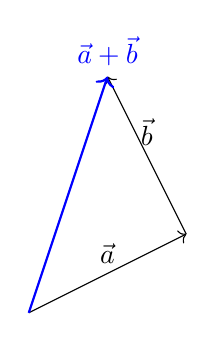
\begin{tikzpicture}
		\draw[->] (0,0) -- (2,1) node[midway, above] {\(\vec{a}\)};
		\draw[->] (2,1) -- (1,3) node[midway, above] {\(\vec{b}\)};
		\draw[->, thick, blue] (0,0) -- (1,3) node[above, above] {\(\vec{a} + \vec{b}\)};
	\end{tikzpicture}
	\caption{Vector addition: \(\vec{a} + \vec{b}\)}
\end{figure}

\subsection{Equation of a Line}

A line is defined by a point \(\vec{P}\) and a direction vector \(\vec{v}\):

\[
	\vec{r}(t) = \vec{P} + t\vec{v}, \quad t \in \Reals
\]

\subsection{Equation of a Plane}

A plane is defined by a point \(\vec{P}\) and a normal vector \(\vec{n}\):

\[
	P: \vec{x} = \vec{s} + \lambda_1 \vec{v_1} + \lambda_2 \vec{v_2}
\]

\subsection{Scalar (Dot) Product}

The inner product of vectors \(\vec{a}\) and \(\vec{b}\) is a function \(\langle x, y\rangle :=V \times V \rightarrow \mathbb{K}\)
with the following properties:

\(\forall \vec{a}, \vec{b} \in V\):

\begin{itemize}
	\item \(\langle\vec{a}, \vec{b}\rangle = \langle\vec{b}, \vec{a}\rangle \)
	\item \(\langle\vec{a}, \vec{b} + \vec{c}\rangle = \langle\vec{a}, \vec{b}\rangle + \langle\vec{a}, \vec{c}\rangle\)
	\item \(\langle\vec{a}, \lambda \vec{b}\rangle = \lambda \langle\vec{a}, \vec{b}\rangle\)
	\item \(\langle\vec{a}, \vec{b}\rangle = 0 \Leftrightarrow \vec{a} = \vec{0} \vee \vec{b} = \vec{0}\)
\end{itemize}

Formula:

\[
	\langle\vec{a}, \vec{b}\rangle = a_1 b_1 + a_2 b_2 + \cdots + a_n b_n = \sum_{i = 1}^{n} a_i b_i
\]

\textbf{Proof:}

Let us look at the following Triangle:

\begin{center}
	\begin{tikzpicture}
		\draw [<->](0, 3) -- (0, -3);
		\draw [<->](3, 0) -- (-3, 0);
		\draw [->, red] (0, 0) -- (2, 2) node[above]{\(\vec{v}\)};
		\draw [->, blue] (0, 0) -- (2, 0) node[above right]{\(\vec{u}\)};
		\draw [->] (2,0) -- (2,2) node[midway, right]{\(\vec{v} - \vec{u}\)};
	    \draw [green, thick] (0.5,0) arc (0:45:0.5) node[midway, right] {\(\theta = 45\)};
	\end{tikzpicture}
\end{center}

We can use the Cosine law: \(\|v - u\|^{2} = \|v\|^2 + \|u\|^2  - 2 \|u\| \|v\| \cos\theta\).
\vspace{\baselineskip}

Now we expand:

\[
	\|u\|^2 = u_{1}^2 + u_{2}^2\ \text{ and } \|v\|^2 = v_{1}^2 + v_{2}^2
\]

Then: \(\|v - u\|^2 = {(v_1 - u_1)}^2 + {(v_2 - u_2)}^2\) and by re-grouping after expansion we get

\[
	\langle v, u\rangle = v_1u_1 + v_2u_2 = \|v\|\|u\|\cos \theta \\ 
\]

\QED

And if we manipulates this expression we can also prove the angle formulas.
And with that information we can prove that

\[
	\cos \frac{\pi}{2}\ = \frac{\langle v, u\rangle}{\|v\|\|u\|} = 0
\]

Only if the Dot Product is equal to zero so, like that we have also proved that
only orthogonal vector have a dot product of zero.

\subsection{Length (Norm) of a Vector}

The norm of a vector \(\vec{a}\) is described by different norms:

It also has the following properties:

\begin{itemize}

	\item \(\|\vec{a}\| \geq 0\) and \(\|\vec{a}\| = 0 \Leftrightarrow \vec{a} = \vec{0}\)

	\item \(\|\lambda \vec{a}\| = |\lambda| \|\vec{a}\|\)

	\item \(\|\vec{a} + \vec{b}\| \leq \|\vec{a}\| + \|\vec{b}\|\) (Triangle inequality)

	\item \(\|\vec{a} + \vec{b}\|^2 = \|\vec{a}\|^2 + \|\vec{b}\|^2 + 2\langle\vec{a}, \vec{b}\rangle\) (Pythagorean theorem)

\end{itemize}

These are the most common norms, although we will be using primarily the euclidean norm:

\begin{itemize}
	\item \emph{Euclidean norm}:
	      \[
		      \|\vec{a}\| = \sqrt{\langle\vec{a}, \vec{a}\rangle} = \sqrt{a_1^2 + a_2^2 + \cdots + a_n^2}
	      \]
	\item \emph{Manhattan norm}:
	      \[
		      \|\vec{a}\|_1 = |a_1| + |a_2| + \cdots + |a_n|
	      \]
	\item \emph{Maximum norm}:
	      \[
		      \|\vec{a}\|_\infty = \max(|a_1|, |a_2|, \dots , |a_n|)
	      \]
\end{itemize}

\subsection{Angle Relations}

The angle \(\theta\) between two vectors is:

\[
	\cos\theta = \frac{\langle\vec{a}, \vec{b}\rangle}{\|\vec{a}\|\|\vec{b}\|}, \quad \theta = \arccos\left( \frac{\langle\vec{a}, \vec{b}\rangle}{\|\vec{a}\|\|\vec{b}\|} \right)
\]

\subsubsection{Line-Line Angle}

Use direction vectors \(\vec{v}_1\) and \(\vec{v}_2\):

\[
	\theta = \arccos\left( \frac{\langle\vec{v}_1, \vec{v}_2\rangle}{\|\vec{v}_1\|\|\vec{v}_2\|} \right)
\]

\subsubsection{Line-Plane Angle}

Let \(\vec{v}\) be the line's direction and \(\vec{n}\) the plane's normal:

\[
	\theta = \arcsin\left( \frac{\langle\vec{v}, \vec{n}\rangle}{\|\vec{v}\|\|\vec{n}\|} \right)
\]

\subsubsection{Plane-Plane Angle}

Angle between planes is angle between their normals:

\[
	\theta = \arccos\left( \frac{\langle\vec{n}_1, \vec{n}_2\rangle}{\|\vec{n}_1\|\|\vec{n}_2\|} \right)
\]

\subsection{Line Relations}

Two lines can be:

\begin{itemize}

	\item \emph{Identical}: same direction vector and point

	\item \emph{Parallel}: direction vectors are proportional

	\item \emph{Intersecting}: one solution for \(t_1\), \(t_2\) such that \(\vec{r}_1(t_1) = \vec{r}_2(t_2)\)

	\item \emph{Skew}: not parallel, do not intersect

\end{itemize}

To find the relation:

\begin{enumerate}

	\item Check if direction vectors are scalar multiples \(\Rightarrow\) parallel

	\item Solve \(\vec{P}_1 + t\vec{v}_1 = \vec{P}_2 + s\vec{v}_2\) for \(t\) and \(s\):

	\begin{itemize}

		\item Solution exists \(\Rightarrow\) intersect

		\item No solution \(\Rightarrow\) skew

	\end{itemize}

	\item If same point and direction vector \(\Rightarrow\) identical

\end{enumerate}

\subsection{Normalization of a vector}

To normalize a vector \(\vec{a}\), we divide it by its length:

\[
	\hat{\vec{a}} = \frac{\vec{a}}{\|\vec{a}\|} = \frac{\begin{pmatrix} a_x \\ a_y \\ a_z \end{pmatrix}}{\sqrt{a_x^2 + a_y^2 + a_z^2}} = \begin{pmatrix} \frac{a_x}{\|\vec{a}\|} \\ \frac{a_y}{\|\vec{a}\|} \\ \frac{a_z}{\|\vec{a}\|} \end{pmatrix}
\]

\subsection{Orthogonal Vectors and the Orthogonal Projection}

Two vectors \(\vec{a}\) and \(\vec{b}\) are orthogonal if:

\[
	\langle\vec{a}, \vec{b}\rangle = 0
\]

The orthogonal projection of vector \(\vec{a}\) onto vector \(\vec{b}\) is given by:

\[
	\text{p}_{\vec{b}}(\vec{a}) = \frac{\langle\vec{a}, \vec{b}\rangle}{\|\vec{b}\|^2} \cdot \vec{b}
\]

\textbf{Proof of the projection formula}

\begin{align*}
	p \| q \implies \alpha q &= p\ \forall \alpha \in \mathbb{K}\ \text{and}\ \forall\ p, q \in V\\
	\langle a - p, q\rangle &= 0 \implies \langle a - \alpha q, q\rangle = 0 \implies \langle a, q\rangle - \alpha \langle q, q\rangle = 0\\
	\alpha &= \frac{\langle a, q\rangle}{\langle q, q\rangle}
\end{align*}


Therefore, the orthogonal projection of vector \(\vec{a}\) on \(\vec{b}\) is given by
multiplying \(\vec{b}\) by the scalar \(\alpha\).

\QED

\begin{figure}[H]
	\centering
	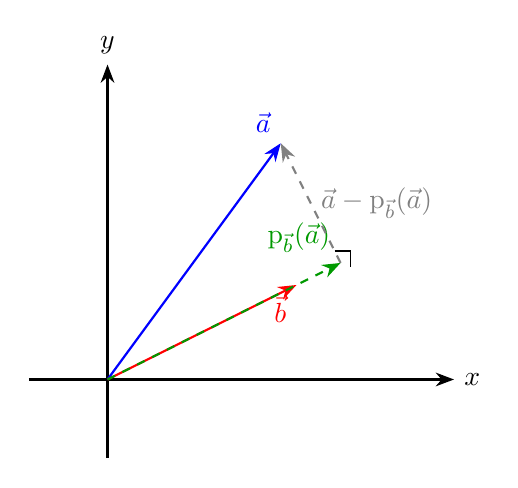
\begin{tikzpicture}[scale=2, >=Stealth]

		% Axes
		\draw[->, thick] (-0.5, 0) -- (2.2, 0) node[right] {\(x\)};
		\draw[->, thick] (0, -0.5) -- (0, 2) node[above] {\(y\)};

		% Coordinates
		\coordinate (O) at (0,0);
		\coordinate (A) at (1.1,1.5);       % vector a
		\coordinate (B) at (1.2,0.6);       % vector b
		\coordinate (P) at (1.48,0.74);     % projection of a onto b

		% Vectors
		\draw[->, thick, blue] (O) -- (A) node[above left] {\(\vec{a}\)};
		\draw[->, thick, red] (O) -- (B) node[below left] {\(\vec{b}\)};
		\draw[->, thick, green!60!black, dashed] (O) -- (P) node[above left] {\(\text{p}_{\vec{b}}(\vec{a})\)};

		% Orthogonal component
		\draw[->, thick, gray, dashed] (P) -- (A) node[midway, right] {\(\vec{a} - \text{p}_{\vec{b}}(\vec{a})\)};

		% Right angle marker
		\draw ($(P)!0.1!(A)$) -- ++(0.1,0) -- ++(0,-0.1);

	\end{tikzpicture}
	\caption{Orthogonal projection of \(\vec{a}\) onto \(\vec{b}\)}
\end{figure}

\subsection{The Cross Product}

The cross product of two vectors \(\vec{a}\) and \(\vec{b}\) in \(\Reals^3\) is defined as:

\[
	\vec{a} \times \vec{b} = \begin{pmatrix} a_1 \\ a_2 \\ a_3 \end{pmatrix} \times \begin{pmatrix} b_1 \\ b_2 \\ b_3 \end{pmatrix} = \begin{pmatrix} a_2 b_3 - a_3 b_2 \\ a_3 b_1 - a_1 b_3 \\ a_1 b_2 - a_2 b_1 \end{pmatrix}
\]

or 

\[
	\det\left( \begin{bmatrix}
		\imath & v_1 & w_1 \\
		\jmath & v_2 & w_2 \\
		\hat{k} & v_3 & w_3
	\end{bmatrix} \right)
	= \imath (v_2 w_3 - v_3 w_2) - \jmath (v_1 w_3 - v_3 w_1) + \hat{k}(v_1 w_2 - v_2 w_1)
\]


The cross product has the following properties:

\begin{itemize}

	\item \(\vec{a} \times \vec{b} = -(\vec{b} \times \vec{a})\)

	\item \(\vec{a} \times (\vec{b} + \vec{c}) = \vec{a} \times \vec{b} + \vec{a} \times \vec{c}\)

	\item \((\lambda_1\vec{a}) \times (\lambda_2\vec{b}) = \lambda_1\lambda_2(\vec{a} \times \vec{b})\)

	\item \(\|\vec{a} \times \vec{b}\| = \|\vec{a}\|\|\vec{b}\| \sin(\theta)\)

	\item \(\langle\vec{a}, (\vec{b} \times \vec{c})\rangle = 0\) (scalar triple product)

	\item \(\vec{a} \times \vec{b} = \vec{0} \Leftrightarrow \vec{a} = \lambda\vec{b}\) for some \(\lambda \in \Reals\) (parallel vectors)

	\item \(\vec{a} \times \vec{b} = \vec{0} \Leftrightarrow \vec{a} = \vec{0} \vee \vec{b} = \vec{0}\) (zero vector)

\end{itemize}

The cross product is not defined in \(\Reals^2\).
The cross product is not commutative, but it is associative:

\[
	(\vec{a} \times \vec{b}) \times \vec{c} = \vec{a} \times (\vec{b} \times \vec{c})
\]

The cross product is distributive over vector addition:

\[
	\vec{a} \times (\vec{b} + \vec{c}) = \vec{a} \times \vec{b} + \vec{a} \times \vec{c}
\]

The cross product is anti-commutative:

\[
	\vec{a} \times \vec{b} = -(\vec{b} \times \vec{a})
\]

The cross product is not associative:

\[
	(\vec{a} \times \vec{b}) \times \vec{c} \neq \vec{a} \times (\vec{b} \times \vec{c})
\]

The cross product is not distributive over scalar multiplication:

\[
	\lambda(\vec{a} \times \vec{b}) \neq (\lambda\vec{a}) \times \vec{b}
\]

The length of the cross product in \(\Reals^3\) is the area of the parallelogram spanned by the two vectors:

\subsection{Orthogonal vectors in \texorpdfstring{\(\Reals^2\ \Reals^3\)}{}}

\subsubsection{Orthogonal vectors in \texorpdfstring{\(\Reals^2\)}{}}

\begin{enumerate}
	\item Interchange the components
	\item Change the sign of one component
\end{enumerate}

\subsubsection{Orthogonal vectors in \texorpdfstring{\(\Reals^3\)}{}}
\begin{enumerate}
	\item Interchange two components
	\item the one that was not changed, set to zero
	\item Change the sign of first component
\end{enumerate}

\textbf{Example:}

\[
	\vec{a} = \begin{pmatrix} 1 \\ 2 \\ 3 \end{pmatrix}, \quad \vec{b} = \begin{pmatrix} -2 \\ 1 \\ 0 \end{pmatrix}
\]

\subsection{Hessian Normal Form}

The Hessian normal form is a way of expressing the equation of a plane in three-dimensional space using a normalized normal vector. It is particularly useful in computational geometry and physics, where signed distances from points to planes are important.

\subsubsection{Geometric Interpretation}

The Hessian normal form represents a plane by specifying:

\begin{itemize}
	
	\item A unit normal vector \(\vec{n} = (a, b, c)\) to the plane,

	\item and the shortest distance \(d\) from the origin to the plane.

\end{itemize}

This form is derived by normalizing the general plane equation. A plane in 3D can be written as:

\[
	ax + by + cz + d = 0,
\]

where \((a, b, c)\) is a normal vector to the plane and \(d\) is the dot product of the normal vector with a point \(p\).
If we divide all terms by \(\sqrt{a^2 + b^2 + c^2}\), we normalize the normal vector:

\[
	\frac{a}{\sqrt{a^2 + b^2 + c^2}}x + \frac{b}{\sqrt{a^2 + b^2 + c^2}}y + \frac{c}{\sqrt{a^2 + b^2 + c^2}}z + \frac{d}{\sqrt{a^2 + b^2 + c^2}} = 0.
\]

Let:

\[
	\vec{n} = \left(\frac{a}{\sqrt{a^2 + b^2 + c^2}}, \frac{b}{\sqrt{a^2 + b^2 + c^2}}, \frac{c}{\sqrt{a^2 + b^2 + c^2}}\right), \quad d' = \frac{d}{\sqrt{a^2 + b^2 + c^2}},
\]

then the equation becomes:

\[
	\vec{n} \cdot \vec{r} + d' = 0,
\]

which is the Hessian normal form. Here, \(\vec{r} = (x, y, z)\) is any point on the plane, and \(\vec{n}\) is the unit normal.

\subsubsection{Signed Distance to the Plane}

This form allows easy calculation of the signed distance from any point \(\vec{p}\) to the plane:

\[
	\text{distance} = \vec{n} \cdot \vec{p} + d',
\]

which is positive if \(\vec{p}\) lies on the same side of the plane as the normal vector.

\subsubsection{Derivation Illustration}

To visualize the derivation, imagine a plane with unit normal vector \(\vec{n}\), and a point \(P\) in space. The shortest distance from \(P\) to the plane is the projection of the vector \(\vec{p} - \vec{q}\) onto \(\vec{n}\), where \(\vec{q}\) is any point on the plane. This leads to:

\[
	\text{distance} = (\vec{p} - \vec{q}) \cdot \vec{n}.
\]

This gives the signed distance formula and thus, motivates the Hessian form.

\subsection{Converting from the parametric form to the Hessian normal form}

Steps:

\begin{enumerate}

	\item Find the normal vector \(\vec{n}\) of the plane
	
	\item Normalize the normal vector
	
	\item Find the distance \(d\) from the origin to the plane
	
	\item Write the Hessian normal form

\end{enumerate}

\subsection{Converting from the Hessian normal form to the parametric form}

Steps:

\begin{enumerate}

	\item Find a point on the plane

	\item Find two direction vectors in the plane

	\item Write the parametric form

\end{enumerate}

\subsection{Properties of lines and planes}

\begin{itemize}

	\item Two planes are parallel if their normal vectors are scalar multiples of each other.

	\item A line and a plane are parallel if the direction vector of the line is orthogonal to the normal vector of the plane.

	\item A line intersects a plane if there exists a point on the line that satisfies the equation of the plane.

	\item Two planes intersect in a line if their normal vectors are not parallel.

	\item Three planes can intersect in a point, a line, or not at all.

	\item If we have a line \(G\) and a point on the line, for every vector \(\vec{n}\) that is orthogonal to the
 	      direction vector of the line: \(x \in G \iff \langle x, n \rangle\)

	\item If \(p\) and \(q\) are two points in the line \(G\) with a normal vector then \(\langle p, n\rangle = \langle q, n\rangle\)

	\item Let \(E\) be a plane with the origin \(p\) and the direction vector \(\vec{v}\) and \(\vec{w}\), then there exist a normal vector and
	      \(x \in E \iff \langle x, n\rangle = \langle p, n \rangle\)

\end{itemize}

\subsection{Convert Normal Vector in Two Direction Vectors}

Steps:

\begin{enumerate}
	
	\item Given the normal vector \(\vec{n} = (a, b, c)\), interchange \(a\) and \(b\) and multiply \(b\) by -1
	
	\item Set the other component to 0. This gives you the first direction vector \(\vec{v} = (-b, a, 0)\)
	
	\item Take the original normal vector \(\vec{n}\) and interchange \(a\) and \(c\) and multiply \(c\) by -1
	
	\item Set the other component to 0. This gives you the second direction vector \(\vec{w} = (-c, 0, a)\)

\end{enumerate}

\subsection{Intersection between Line and Plane}

To find the intersection between a line and a plane, we can use the following steps:

\begin{enumerate}

	\item Write the parametric form of the line: \(\vec{r}(t) = \vec{P} + t\vec{v}\), where \(\vec{P}\) is a point on the line and \(\vec{v}\) is the direction vector.

	\item Write the equation of the plane in Hessian normal form: \(\langle \vec{n}, \vec{x} - \vec{P} \rangle = 0\), where \(\vec{n}\) is the normal vector and \(\vec{P}\) is a point on the plane.

	\item Substitute the parametric form of the line into the equation of the plane.

	\item Solve for \(t\) to find the intersection point.

	\item Substitute \(t\) back into the parametric form of the line to find the intersection point.

\end{enumerate}

\textbf{Example:}
\vspace{\baselineskip}

Given the line:

\[
	g(t) = \begin{pmatrix} 0 \\ 0 \\ 1 \end{pmatrix} + t \begin{pmatrix} 1 \\ 1 \\ 1 \end{pmatrix}
\]

and the plane:

\[
	E(u, m) = \begin{pmatrix} 0 \\ 1 \\ 2 \end{pmatrix} + u \begin{pmatrix} 1 \\ 0 \\ 1 \end{pmatrix} + m \begin{pmatrix} 1 \\ 1 \\ 0 \end{pmatrix},
\]

we want to find the intersection point.

\textbf{Step 1:} Determine the normal vector of the plane using the cross product of the two direction vectors:

\[
	\vec{v}_1 = \begin{pmatrix} 1 \\ 0 \\ 1 \end{pmatrix}, \quad \vec{v}_2 = \begin{pmatrix} 1 \\ 1 \\ 0 \end{pmatrix}
\]

\[
	\vec{n} = \vec{v}_1 \times \vec{v}_2 =
	\begin{pmatrix} 1 \\ 0 \\ 1 \end{pmatrix} \times \begin{pmatrix} 1 \\ 1 \\ 0 \end{pmatrix} =
	\begin{pmatrix} -1 \\ 1 \\ 1 \end{pmatrix}
\]

\textbf{Step 2:} Use the normal vector and a point on the plane to write the plane equation:

\[
	\langle \vec{n}, \vec{x} - \vec{Q} \rangle = 0, \quad \vec{Q} = \begin{pmatrix} 0 \\ 1 \\ 2 \end{pmatrix}
\]

\textbf{Step 3:} Plug the line into the plane equation:

\[
	\vec{x}(t) = \begin{pmatrix} 0 \\ 0 \\ 1 \end{pmatrix} + t \begin{pmatrix} 1 \\ 1 \\ 1 \end{pmatrix}
	\Rightarrow
	\vec{x}(t) - \vec{Q} =
	\begin{pmatrix} t \\ t - 1 \\ t - 1 \end{pmatrix}
\]

Now compute the dot product:

\[
	\langle \vec{n}, \vec{x}(t) - \vec{Q} \rangle =
	\begin{pmatrix} -1 \\ 1 \\ 1 \end{pmatrix} \cdot \begin{pmatrix} t \\ t - 1 \\ t - 1 \end{pmatrix}
	= -t + (t - 1) + (t - 1) = t - 2
\]

\textbf{Step 4:} Solve for \(t\):

\[
	t - 2 = 0 \Rightarrow t = 2
\]

\textbf{Step 5:} Substitute \( t = 2 \) into the line:

\[
	\vec{x}(2) = \begin{pmatrix} 0 \\ 0 \\ 1 \end{pmatrix} + 2 \begin{pmatrix} 1 \\ 1 \\ 1 \end{pmatrix} =
	\begin{pmatrix} 2 \\ 2 \\ 3 \end{pmatrix}
\]

\textbf{Result:} The line intersects the plane at the point

\[
	\boxed{\begin{pmatrix} 2 \\ 2 \\ 3 \end{pmatrix}}
\]

\textbf{Proof:}

\[
	E: \langle x, n\rangle = \langle p, n \rangle
\]
\[
	G: x = p + t \cdot v
\]
\[
	\langle x, n \rangle = c
\]
\[
	\langle p + t \cdot v, n \rangle = c
\]
\[
	\langle p, n \rangle + t \cdot \langle v, n \rangle = c
\]
\[
	t = \frac{c - \langle p, n \rangle}{\langle v, n \rangle}
\]
\QED

\subsection{Distances between points, lines and planes}

\subsubsection{Distance between two points}

The distance between two points \(\vec{P_1}\) and \(\vec{P_2}\) in \(\Reals^n\) is given by:
\[
	d(\vec{P_1}, \vec{P_2}) = \|\vec{P_1} - \vec{P_2}\| = \sqrt{{(x_1 - x_2)}^2 + {(y_1 - y_2)}^2 + \cdots + {(z_1 - z_2)}^2}
\]
where \(\vec{P_1} = (x_1, y_1, \dots,z_1)\) and \(\vec{P_2} = (x_2, y_2, \dots,z_2)\).

\subsubsection{Distance between a point and a hyperplane}

The distance between a point \(\vec{P}\) and a hyperplane defined by the equation \(\langle \vec{n}, \vec{x} - \vec{P_0} \rangle = 0\) is given by:

\[
	d(\vec{P}, \text{hyperplane}) = \frac{|\langle \vec{n}, \vec{P} - \vec{P_0} \rangle|}{\|\vec{n}\|}
\]

where \(\vec{P_0}\) is a point on the hyperplane and \(\vec{n}\) is the normal vector of the hyperplane.

\subsubsection{Distance between two lines}

The distance between two lines in \(\Reals^3\) can be calculated using the formula:

\[
	d = \frac{|\langle \vec{v_1} \times \vec{v_2}, \vec{P_2} - \vec{P_1} \rangle|}{\|\vec{v_1} \times \vec{v_2}\|}
\]

where \(\vec{P_1}\) and \(\vec{P_2}\) are points on the two lines, and \(\vec{v_1}\) and \(\vec{v_2}\) are the direction vectors of the lines.

\subsubsection{Distance between a point and a line}

The distance between a point \(\vec{P}\) and a line defined by the parametric equation \(\vec{r}(t) = \vec{P_0} + t\vec{v}\) is given by:

\[
	d(\vec{P}, \text{line}) = \frac{\|\vec{v} \times (\vec{P} - \vec{P_0})\|}{\|\vec{v}\|}
\]

where \(\vec{P_0}\) is a point on the line and \(\vec{v}\) is the direction vector of the line.

\subsubsection{Distance between two planes}

The distance between two parallel planes defined by the equations \(\langle \vec{n}, \vec{x} - \vec{P_1} \rangle = 0\) and \(\langle \vec{n}, \vec{x} - \vec{P_2} \rangle = 0\) is given by:

\[
	d = \frac{|\langle \vec{n}, \vec{P_2} - \vec{P_1} \rangle|}{\|\vec{n}\|}
\]

where \(\vec{P_1}\) and \(\vec{P_2}\) are points on the two planes, and \(\vec{n}\) is the normal vector of the planes.

\subsubsection{Distance between a point and a plane}

The distance between a point \(\vec{P}\) and a plane defined by the equation \(\langle \vec{n}, \vec{x} - \vec{P_0} \rangle = 0\) is given by:

\[
	d(\vec{P}, \text{plane}) = \frac{|\langle \vec{n}, \vec{P} - \vec{P_0} \rangle|}{\|\vec{n}\|}
\]

where \(\vec{P_0}\) is a point on the plane and \(\vec{n}\) is the normal vector of the plane.
\vspace{\baselineskip}

\textbf{Example:}
\vspace{\baselineskip}
 
Distance Between Two Skew Lines

To find the shortest distance between two skew lines, we use the formula:

\[
	\text{distance} = \frac{|\langle(\vec{P}_2 - \vec{P}_1), (\vec{v}_1 \times \vec{v}_2)\rangle|}{\|\vec{v}_1 \times \vec{v}_2\|}
\]

Where:

\begin{itemize}

	\item \(\vec{P}_1\) and \(\vec{P}_2\) are points on each line,

	\item \(\vec{v}_1\) and \(\vec{v}_2\) are the direction vectors,

	\item \(\vec{v}_1 \times \vec{v}_2\) is the cross product of the direction vectors.

\end{itemize}

\textbf{Given:}

\[
	g_1: \vec{r}_1(a) = \begin{pmatrix} 2 \\ 2 \\ 2 \end{pmatrix} + a \begin{pmatrix} 0 \\ 1 \\ 1 \end{pmatrix}, \quad
	g_2: \vec{r}_2(b) = \begin{pmatrix} 1 \\ 2 \\ 3 \end{pmatrix} + b \begin{pmatrix} 3 \\ 2 \\ 1 \end{pmatrix}
\]

\textbf{Step 1:} Set

\[
	\vec{P}_1 = \begin{pmatrix} 2 \\ 2 \\ 2 \end{pmatrix}, \quad \vec{v}_1 = \begin{pmatrix} 0 \\ 1 \\ 1 \end{pmatrix}
\]
\[
	\vec{P}_2 = \begin{pmatrix} 1 \\ 2 \\ 3 \end{pmatrix}, \quad \vec{v}_2 = \begin{pmatrix} 3 \\ 2 \\ 1 \end{pmatrix}
\]

\textbf{Step 2:} Compute the vector between base points:

\[
	\vec{P}_2 - \vec{P}_1 = \begin{pmatrix} 1 - 2 \\ 2 - 2 \\ 3 - 2 \end{pmatrix} = \begin{pmatrix} -1 \\ 0 \\ 1 \end{pmatrix}
\]

\textbf{Step 3:} Compute the cross product:

\[
	\vec{v}_1 \times \vec{v}_2 =
	\begin{pmatrix} 1 \\ 1 \\ 0 \end{pmatrix} \times \begin{pmatrix} 3 \\ 2 \\ 1 \end{pmatrix}
	= \begin{pmatrix}
		(1)(1) - (1)(2) \\
		(1)(3) - (0)(1) \\
		(0)(2) - (1)(3)
	\end{pmatrix}
	= \begin{pmatrix}
		-1 \\ 3 \\ -3
	\end{pmatrix}
\]

\textbf{Step 4:} Compute scalar triple product:

\[
	\langle(\vec{P}_2 - \vec{P}_1), (\vec{v}_1 \times \vec{v}_2)\rangle =
	\langle\begin{pmatrix} -1 \\ 0 \\ 1 \end{pmatrix}, \begin{pmatrix} -1 \\ 3 \\ -3 \end{pmatrix}\rangle
	= (-1)(-1) + (0)(3) + (1)(-3) = 1 + 0 - 3 = -2
	\Rightarrow |\dots| = 2
\]

\textbf{Step 5:} Magnitude of the cross product:

\[
	\|\vec{v}_1  \vec{v}_2\|= \sqrt{(-1)^2 + 3^2 + (-3)^2} = \sqrt{1 + 9 + 9} = \sqrt{19}
\]

\textbf{Final Answer:}

\[
	\text{distance} = \frac{2}{\sqrt{19}} \approx 0.458
\]

\[
text{Shortest distance between the lines is } \frac{2}{\sqrt{19}}
\]

\subsection{Foot of the Perpendicular and Mirror Point}

\subsubsection{Foot of the Perpendicular}

The \emph{foot of the perpendicular} from a point \(\vec{P}\) to a line (or plane) is the point on the line (or plane) where the perpendicular from \(\vec{P}\) meets it.
\vspace{\baselineskip}

\textbf{Line case:}

Given a line in parametric form:

\[
	g: \vec{r}(t) = \vec{A} + t\vec{v}
\]

and a point \(\vec{P}\) not on the line, the foot of the perpendicular \(\vec{F}\) satisfies:

\[
	(\vec{P} - \vec{F}) \perp \vec{v} \quad \Rightarrow \quad (\vec{P} - (\vec{A} + t\vec{v})) \cdot \vec{v} = 0
\]

Solve this inner product for \(t\), then compute:

\[
	\vec{F} = \vec{A} + t\vec{v}
\]

\textbf{Plane case:}

Given a plane in normal form:

\[
	\langle \vec{n}, \vec{x} - \vec{Q} \rangle = 0
\]

then the foot of the perpendicular from point \(\vec{P}\) to the plane is:

\[
	\vec{F} = \vec{P} - ((\vec{P} - \vec{Q}) \cdot \vec{n}) \cdot \vec{n}
\]

\subsubsection{Mirror Point}

The \emph{mirror point} (or reflected point) of \(\vec{P}\) across a line or plane is the point \(\vec{P}'\) such that the midpoint between \(\vec{P}\) and \(\vec{P}'\) is the foot of the perpendicular.

\textbf{Formula:}

\[
	\vec{P}' = 2\vec{F} - \vec{P}
\]

Where \(\vec{F}\) is the foot of the perpendicular from \(\vec{P}\) to the line or plane.

\section{Algebraic Structures}

\subsection{Introduction}

Algebraic structures are mathematical systems consisting of a set equipped with one or more operations that satisfy certain axioms. They provide a unified language to study various objects in mathematics, from numbers and matrices to functions and vector spaces. Understanding these structures is fundamental in abstract algebra and has applications in computer science, cryptography, coding theory, and physics.

\subsection{Operations: Internal and External}

An \textbf{internal composition law} is a binary operation that takes two elements from a set and returns another element in the same set. Formally, for a set \(S\) and operation \(\circ\), we have:
\[
\circ: S \times S \rightarrow S
\]

An \textbf{external composition law} involves a second set acting on the structure, such as scalar multiplication in vector spaces:
\[
\cdot: K \times V \rightarrow V
\]
where \(K\) is a field and \(V\) is a vector space.

\subsection{Properties of Operations}

Let \(\ast\) be a binary operation on a set \(S\). The most important properties include:

\begin{itemize}[label=\(-\)]
    \item \textbf{Associativity:} \((a \ast b) \ast c = a \ast (b \ast c)\) for all \(a,b,c \in S\)
    \item \textbf{Commutativity:} \(a \ast b = b \ast a\) for all \(a,b \in S\)
    \item \textbf{Identity Element:} There exists \(e \in S\) such that \(a \ast e = e \ast a = a\) for all \(a \in S\)
    \item \textbf{Inverse Element:} For every \(a \in S\), there exists \(a^{-1} \in S\) such that \(a \ast a^{-1} = a^{-1} \ast a = e\)
    \item \textbf{Distributivity:} \(a \circ (b \bullet c) = (a \circ b) \bullet (a \circ c)\) and/or \((b \bullet c) \circ a = (b \circ a) \bullet (c \circ a)\)
\end{itemize}

\subsection{Homomorphisms and Isomorphisms}

Let \((G, \oplus)\) and \((H, \oplus')\) be two algebraic structures.

\begin{itemize}[label=\(-\)]
    \item A \textbf{homomorphism} is a function \(\varphi: G \rightarrow H\) such that:
    \[
    \varphi(a \oplus b) = \varphi(a) \oplus' \varphi(b), \quad \forall a,b \in G
    \]
    
    \item An \textbf{isomorphism} is a bijective homomorphism. If such a map exists, we say the structures are \textbf{isomorphic}, written as \(G \cong H\).
\end{itemize}

\subsection{Common Algebraic Structures}

The following table lists common algebraic structures along with their notation and defining properties. Let \(\oplus\) denote the additive operation and \(\odot\) the multiplicative one:

\begin{center}
\renewcommand{\arraystretch}{1.4}
\begin{tabular}{|c|c|l|}
\hline
\textbf{Name} & \textbf{Notation} & \textbf{Properties} \\
\hline
\textbf{Semigroup} & \((S, \oplus)\) & Associative \\
\hline
\textbf{Monoid} & \((M, \oplus)\) & Associative, Identity element \\
\hline
\textbf{Group} & \((G, \oplus)\) & Associative, Identity, Inverses \\
\hline
\textbf{Abelian Group} & \((A, \oplus)\) & Group + Commutativity \\
\hline
\textbf{Ring} & \((R, \oplus, \odot)\) & \begin{tabular}[c]{@{}l@{}}\((R, \oplus)\) is an abelian group,\\ \((R, \odot)\) is a semigroup,\\ Distributivity: \(a \odot (b \oplus c) = a \odot b \oplus a \odot c\)\end{tabular} \\
\hline
\textbf{Commutative Ring} & \((R, \oplus, \odot)\) & Ring + \((R, \odot)\) is commutative \\
\hline
\textbf{Field} & \((K, \oplus, \odot)\) & \begin{tabular}[c]{@{}l@{}}Commutative Ring +\\ \((K \setminus \{0\}, \odot)\) is an abelian group\end{tabular} \\
\hline
\textbf{Vector Space} & \((V, \oplus, \cdot)\) & \begin{tabular}[c]{@{}l@{}}\((V, \oplus)\) is an abelian group,\\ \(\cdot: K \times V \to V\) (scalar mult.),\\ Distributivity, associativity, identities\end{tabular} \\
\hline
\end{tabular}
\end{center}

\newpage

\newpage
\section{Vector Spaces}

A \emph{vector space} is a set \(V\) with two operations, vector addition and scalar multiplication, 
such that:

\begin{enumerate}[label=\Roman*.]

	\item The set \(V\) is closed under vector addition.

	\item The set \(V\) is closed under scalar multiplication.

	\item Vector addition is commutative.

	\item Vector addition is associative.

	\item There exists a zero vector \(\vec{0} \in V\) such that \(\vec{v} + \vec{0} = \vec{v}\) 
		  for all \(\vec{v} \in V\).

	\item For every vector \(\vec{v} \in V\), there exists a vector \(-\vec{v} \in V\) such that 
	      \(\vec{v} + (-\vec{v}) = \vec{0}\).

	\item Scalar multiplication is distributive with respect to vector addition: 
	      \(a(\vec{u} + \vec{v}) = a\vec{u} + a\vec{v}\) for all \(a \in F\) and 
		  \(\vec{u}, \vec{v} \in V\).

	\item Scalar multiplication is distributive with respect to field addition: 
	      \((a + b)\vec{v} = a\vec{v} + b\vec{v}\) for all \(a, b \in F\) and \(\vec{v} \in V\).

	\item Scalar multiplication is associative: \(a(b\vec{v}) = (ab)\vec{v}\) for all \(a, b \in F\) 
	      and \(\vec{v} \in V\).

	\item The multiplicative identity acts as a scalar: \(1\vec{v} = \vec{v}\) for all \(\vec{v} \in V\).

\end{enumerate}

The set \(F\) is a field, and the elements of \(V\) are called \emph{vectors}.
\vspace{\baselineskip}

\textbf{Examples:}

\begin{enumerate}

	\item The set of all \(n\)-tuples of real numbers \(\Reals^n\) is a vector space over the field 
	      of real numbers \(\Reals\).

	\item The set of all polynomials of degree less than or equal to \(n\) is a vector space over the 
	      field of real numbers \(\Reals\).

	\item The set of all continuous functions from \(\Reals\) to \(\Reals\) is a vector space 7
	      over the field of real numbers \(\Reals\).

	\item The set of all \(m \times n\) matrices with real entries is a vector space over the field of 
	      real numbers \(\Reals\).

\end{enumerate}

\subsection{Subspaces}

A subset \(W\) of a vector space \(V\) is a \emph{subspace} of \(V\) if:

\begin{enumerate}[label=\Roman*.]

	\item The zero vector \(\vec{0} \in W\).

	\item For all \(\vec{u}, \vec{v} \in W\), \(\vec{u} + \vec{v} \in W\).

	\item For all \(a \in F\) and \(\vec{v} \in W\), \(a\vec{v} \in W\).

\end{enumerate}

If \(W\) is a subspace of \(V\), we write \(W \subseteq V\).
\vspace{\baselineskip}

The intersection of two subspaces is also a subspace.

\subsection{Linear Combinations}

A \emph{linear combination} of vectors \(\vec{v}_1, \vec{v}_2, \ldots, \vec{v}_n\) in a vector space 
\(V\) is an expression of the form:

\[
	a_1\vec{v}_1 + a_2\vec{v}_2 + \cdots + a_n\vec{v}_n
\]

Where \(a_1, a_2, \ldots, a_n\) are scalars from the field \(F\).
The set of all linear combinations of a set of vectors \(\{\vec{v}_1, \vec{v}_2, \ldots, \vec{v}_n\}\) 
is called the \textbf{span} of those vectors, 
denoted by \(\text{span}(\vec{v}_1, \vec{v}_2, \ldots, \vec{v}_n)\). The span of a set of vectors is a 
subspace of the vector space \(V\).
\vspace{\baselineskip}

The span of a set of vectors is the smallest subspace containing those vectors.

\subsection{Properties of the subspaces}

\begin{itemize}

	\item The intersection of two subspaces is a subspace.

	\item The union of two subspaces is not necessarily a subspace.

	\item The sum of two subspaces \(U\) and \(W\) is defined as:
	      \[
		      U + W = \{\vec{u} + \vec{w} : \vec{u} \in U, \vec{w} \in W\}
	      \]
	      The sum of two subspaces is a subspace.

		\end{itemize}

The sum of two subspaces is the smallest subspace containing both subspaces.

\begin{itemize}

	\item The direct sum of two subspaces \(U\) and \(W\) is defined as:
	      \[
		      U \oplus W = \{\vec{u} + \vec{w} : \vec{u} \in U, \vec{w} \in W\}
	      \]
	      The direct sum of two subspaces is a subspace.

	\item The direct sum of two subspaces is the smallest subspace containing both subspaces, such that 
		  \(U \cap W = \{\vec{0}\}\).

	\item The direct sum of two subspaces is denoted by \(U \oplus W\).

\end{itemize}

\subsection{Linear Independence}

A set of vectors \(\{\vec{v}_1, \vec{v}_2, \dots, \vec{v}_n\}\) in a vector space \(V\) is said to 
be \emph{linearly independent} if the only solution to the equation:

\[
	\lambda_1\vec{v}_1 + \lambda_2\vec{v}_2 + \cdots + \lambda_n\vec{v}_n = 0
\]

or

\[
	\sum_{i=1}^n \lambda_i \vec{v}_i = 0
\]

is \(a_1 = a_2 = \cdots = a_n = 0\). If there exists a non-trivial solution to this equation, 
then the set of vectors is said to be linearly dependent. A set of vectors is linearly 
independent if and only if the only linear combination of those vectors that equals the zero vector 
is the trivial combination where all coefficients are zero.

\subsubsection{Properties of the linear independence}

\begin{itemize}

	\item A set of vectors \(\{\vec{v}_1, \vec{v}_2, \ldots, \vec{v}_n\}\) is linearly independent 
	      if and only if the only linear combination of those vectors that equals the zero vector is 
		  the trivial combination where all coefficients are zero.

	\item If a set of vectors \(\{\vec{v}_1, \vec{v}_2, \ldots, \vec{v}_n\}\) is linearly independent, 
	      then any subset of that set is also linearly independent.

	\item If a set of vectors \(\{\vec{v}_1, \vec{v}_2, \ldots, \vec{v}_n\}\) is linearly dependent, 
	      then at least one vector in that set can be expressed as a linear combination of the others.

\end{itemize}

\subsection{Base}

\begin{itemize}

	\item A \emph{base} of a vector space \(V\) is a set of vectors 
	      \(\{\vec{v}_1, \vec{v}_2, \ldots, \vec{v}_n\}\) that is linearly independent and 
		  spans the vector space \(V\).

	\item The number of vectors in a base of a vector space is called the \emph{dimension} of the 
	      vector space.

	\item The dimension of a vector space \(V\) is denoted by \(\dim(V)\).

	\item If \(V\) has a finite base, then it is said to be \emph{finite-dimensional}.

	\item If \(V\) does not have a finite base, then it is said to be \emph{infinite-dimensional}.
\end{itemize}

\subsection{Dimension}

The \emph{dimension} of a vector space \(V\) is the number of vectors in a base of \(V\).

\begin{itemize}

	\item The dimension of a vector space is denoted by \(\dim(V)\).

	\item The dimension of a vector space can be finite or infinite.

	\item If the dimension of a vector space is finite, then it is said to be \emph{finite-dimensional}.

	\item If the dimension of a vector space is infinite, then it is said to be \emph{infinite-dimensional}.

\end{itemize}

\subsubsection{How to find the base of a set vector}

To find the base of a set of vectors, we can use the following steps:

\begin{enumerate}

	\item Write the vectors as columns of a matrix.

	\item Row-reduce the matrix to echelon form.

	\item The non-zero rows of the echelon form matrix correspond to the base of the vector space 
	      spanned by the original set of vectors.

\end{enumerate}

The number of non-zero rows in the echelon form matrix is equal to the dimension of the vector space 
spanned by the original set of vectors.
\vspace{\baselineskip}

The base of a vector space is not unique. Different bases can span the same vector space.

\subsection{Basis Extension Theorem}

Let \(V\) be a vector space over a field \(K\), and let 

\[
	v_1, \ldots, v_r,\quad w_1, \ldots, w_s \in V.
\]

Suppose that \((v_1, \ldots, v_r)\) is a linearly independent tuple and that

\[
	\text{span}(v_1, \ldots, v_r, w_1, \ldots, w_s) = V.
\]

Then it is possible to extend \((v_1, \ldots, v_r)\) to a basis of \(V\) by possibly adding suitable 
vectors from the set \(\{w_1, \ldots, w_s\}\).
\vspace{\baselineskip}

\textbf{Proof:}

If \(\text{span}(v_1, \ldots, v_r) = V\), the statement is obvious. So assume

\[
	\text{span}(v_1, \ldots, v_r) \neq V.
\]

Then there exists at least one \(w_i\) such that \(w_i \notin \text{span}(v_1, \ldots, v_r)\); 
otherwise, if all \(w_i \in \text{span}(v_1, \ldots, v_r)\), then

\[
	\text{span}(v_1, \ldots, v_r, w_1, \ldots, w_s) = \text{span}(v_1, \ldots, v_r) = V,
\]
which contradicts our assumption that \(\text{span}(v_1, \ldots, v_r) \neq V\).

The tuple \((w_i, v_1, \ldots, v_r)\) is linearly independent, because of

\[
	\sum_{j=1}^r \lambda_j v_j + \lambda w_i = 0
\]

It follows that \(\lambda = 0\) (since \(w_i \notin \text{span}(v_1, \ldots, v_r)\)), and then also 
\(\lambda_j = 0\) for all \emph{j} because the \(v_j\) are linearly independent.

Possibly, \((w_i, v_1, \ldots, v_r)\) is still not a basis of \(V\). Then we repeat the previous step and 
keep adding further \(w_i\) until the tuple extends \((v_1, \ldots, v_r)\) to a basis of \(V\). This 
process terminates after finitely many steps, since

\[
	\text{span}(v_1, \ldots, v_r, w_1, \ldots, w_s) = V.
\]

\QED
\vspace{\baselineskip}

Every finitely generated vector space \(V\) has a basis.

\subsection{Exchange Lemma}

Let \((v_1, \ldots, v_n)\) and \((w_1, \ldots, w_m)\) be bases of a vector space \(V\). Then, for every 
\(v_i\), there exists a \(w_j\) such that if we replace \(v_i\) by \(w_j\) in the tuple 
\((v_1, \ldots, v_n)\), it still forms a basis of \(V\).
\vspace{\baselineskip}

\textbf{Proof:}

Let \((v_1, \ldots, v_n)\) and \((w_1, \ldots, w_m)\) be two bases of \(V\). Suppose we remove \(v_i\) 
from the first basis. The truncated tuple \((v_1, \ldots, v_{i-1}, v_{i+1}, \ldots, v_n)\) satisfies

\[
	\text{span}(v_1, \ldots, v_{i-1}, v_{i+1}, \ldots, v_n) \neq V,
\]

because if \(\text{span}(v_1, \ldots, v_{i-1}, v_{i+1}, \ldots, v_n) = V\), then \(v_i\) would lie in the 
span of the remaining vectors and could be written as a linear combination of them. This would contradict 
the assumption that \((v_1, \ldots, v_n)\) is linearly independent and a basis of \(V\).

By the Basis Extension Theorem, we can extend the truncated 
tuple \((v_1, \ldots, v_{i-1}, v_{i+1}, \ldots, v_n)\) to a basis of \(V\) by 
adding vectors from \((v_1, \ldots, v_{i-1}, v_{i+1}, \ldots, v_n, w_1, \ldots, w_m)\). 
Therefore, by the Basis Extension Theorem, there exists a \(w_j\) such that

\[
	w_j \notin \text{span}(v_1, \ldots, v_{i-1}, v_{i+1}, \ldots, v_n),
\]

and the tuple \((v_1, \ldots, v_{i-1}, v_{i+1}, \ldots, v_n, w_j)\) is linearly independent.

If this tuple does not form a basis, we can again apply the Basis Extension Theorem 
and add one of the vectors \(v_1, \ldots, v_n\) to complete the basis. Clearly, the only possibility is 
to add \(v_i\), but this would imply that the tuple \((v_1, \ldots, v_n, w_j)\) is not a basis, as 
\(w_j\) would then be linearly dependent on the other vectors. 
Therefore, \((v_1, \ldots, v_{i-1}, v_{i+1}, \ldots, v_n, w_j)\) must form a basis of \(V\).

\QED

\subsection{Dimension of a sum of subspaces}

Let \(U\) and \(W\) be two subspaces of a vector space \(V\). Then the dimension of the sum of the two 
subspaces is given by:

\[
    \dim(U + W) = \dim(U) + \dim(W) - \dim(U \cap W)    
\]

\subsection{Linear Independence of polynomials}

Let \(P_n\) be the vector space of polynomials of degree at most \(n\). The set of polynomials 
\(\{1, x, x^2, \ldots, x^n\}\) is a basis for \(P_n\).
The dimension of \(P_n\) is \(n + 1\).

\begin{itemize}

	\item The set of polynomials \(\{1, x, x^2, \ldots, x^n\}\) is linearly independent.

	\item The set of polynomials \(\{1, x, x^2, \ldots, x^n\}\) spans the vector space \(P_n\).

	\item The dimension of \(P_n\) is \(n + 1\).

\end{itemize}

To prove that the set of polynomials \(\{1, x, x^2, \ldots, x^n\}\) is linearly independent, 
we can use the following steps:

\begin{enumerate}

	\item Assume that there exists a linear combination of the polynomials that equals zero:   

	\[
	    a_0 + a_1 x + a_2 x^2 + \ldots + a_n x^n = 0,
    \]
 		where \(a_0, a_1, \ldots, a_n\) are scalars.
	
		\item Since the left-hand side is a polynomial of degree at most \(n\), it can only be equal 
			  to zero if all coefficients are zero.
 
		\item Therefore, we have \(a_0 = a_1 = \cdots = a_n = 0\), which 
		 	   proves that the set of polynomials \(\{1, x, x^2, \ldots, x^n\}\) is linearly independent.

\end{enumerate}

So you only have to prove that the set of coefficients vector is linearly independent.

\subsection{Interpolation Polynomial}

Given the \(n+1\) points \((x_k, y_k)\), with \(0 \leq k \leq n\) and all \(x_k\) distinct, 
there exists exactly one polynomial \(p_n \in P_n\) such that \(y_k = p_n(x_k)\) for all \(0 \leq k \leq n\). 
This polynomial is called the interpolation polynomial.
\vspace{\baselineskip}

\textbf{Proof}

The uniqueness follows immediately. We prove the existence by induction on 
\(n\). For \(n = 0\), choose \(p_0(x) = y_0\). 
\vspace{\baselineskip}

Now assume the statement is true for \(n-1\). Let the polynomial \(p_{n-1}\)
interpolate the points \((x_0, y_0), \ldots, (x_{n-1}, y_{n-1})\). 
\vspace{\baselineskip}

Define

\[
	p_n(x) = p_{n-1}(x) + q(x),
\]

where

\[
	q(x) = \frac{(x - x_0)(x - x_1)\cdots(x - x_{n-1})}{(x_n - x_0)(x_n - x_1)\cdots(x_n - x_{n-1})} 
	(y_n - p_{n-1}(x_n)).
\]

We have \(q \in P_n\), and it follows that \(p_n \in P_n\). 
Furthermore, \(q(x_k) = 0\) for \(k \leq n-1\) because a linear factor in 
the numerator always vanishes at \(x_k\). Therefore, \(p_n(x_k) = y_k\) for 
\(k \leq n-1\). Additionally, we have

\[
	q(x_n) = y_n - p_{n-1}(x_n),
\]

so that \(p_n(x_n) = y_n\). 

\QED
\vspace{\baselineskip}

\textbf{Example:}
\vspace{\baselineskip}

Consider the three points \((-2, 1)\), \((-1, -1)\), and \((1, 1)\). 
These points uniquely define an interpolating parabola \(p_2\). This parabola can be 
determined using the definition of \(p_n\). 
For hand calculations and a few 
points to interpolate, the following approach is also useful. The general form of the polynomial is 

\[
	p_2(x) = ax^2 + bx + c.
\]

Substituting the three points into this form gives the system of equations:

\[
	1 = a + b + c \quad \text{(from the point (1, 1))}
\]
\[
	-1 = a - b + c \quad \text{(from the point (-1, -1))}
\]
\[
	1 = 4a - 2b + c \quad \text{(from the point (-2, 1))}
\]

This leads to the system of equations:

\[
	\begin{pmatrix}
	1 & 1 & 1 \\
	1 & -1 & 1 \\
	4 & -2 & 1
	\end{pmatrix}
	\begin{pmatrix}
	a \\
	b \\
	c
	\end{pmatrix}
	=
	\begin{pmatrix}
	1 \\
	-1 \\
	1
	\end{pmatrix}
\]

Solving this system gives \(a = 1\), \(b = 1\), and \(c = -1\), so the interpolation polynomial is
\[
	p_2(x) = x^2 + x - 1.
\]




\newpage
\section{Dot Product, Euclidean and Unitary Space}

\subsection{Scalar Product}

Let \(V\) be a vector space over a field \(K\). A mapping \(\langle \cdot, \cdot \rangle : V \times V \to K\) is called a scalar product (or inner product) if the following conditions are satisfied:
\vspace{\baselineskip}

\emph{Symmetry}

For all \(a, b \in V\):

\[
\langle a, b \rangle = 
\begin{cases}
\langle b, a \rangle & \text{if } K = \mathbb{R}, \\
\overline{\langle b, a \rangle} & \text{if } K = \mathbb{C}.
\end{cases}
\]

\emph{Linearity in the First Argument}

For all \(a, b, c \in V\):

\[
\langle a, b + c \rangle = \langle a, b \rangle + \langle a, c \rangle
\]
and
\[
\langle a + b, c \rangle = \langle a, c \rangle + \langle b, c \rangle.
\]

\emph{Homogeneity in the First Argument}

For all \(\alpha \in K\), we have:

\[
\langle \alpha a, b \rangle = \alpha \langle a, b \rangle = 
\begin{cases}
\langle a, \alpha b \rangle & \text{if } K = \mathbb{R}, \\
\langle a, \alpha b \rangle & \text{if } K = \mathbb{C}.
\end{cases}
\]

\emph{Positive Definiteness}

For all \(a \in V \setminus \{0\}\):

\[
\langle a, a \rangle > 0,
\]
and
\[
\langle 0, 0 \rangle = 0.
\]

\subsection{Standard Scalar Product for Complex Number}

Let \( a = {(a_i)}_{i=1}^n \) and \( b = {(b_i)}_{i=1}^n \) be vectors in \( \mathbb{C}^n \). The standard scalar product is defined by

\[
\langle a, b \rangle := \sum_{i=1}^n a_i b_i.
\]

\subsection{Scalar Product on \texorpdfstring{\( C[a, b] \)}{}}

Let \( f, g \in C[a, b] \). The scalar product on \( C[a, b] \) is defined by

\[
\langle f, g \rangle := \int_a^b f(x) \cdot g(x) \, dx.
\]

\subsection{Euclidean and Unitary Vector Spaces}

A real vector space equipped with a scalar product is called a \textit{Euclidean vector space}, while a complex vector space with a scalar product is called a \textit{unitary vector space}.

\subsection{Norms in Vector Spaces}

Let \( V \) be a \( K \)-vector space and \( a, b \in V \). A function \( \| \cdot \| : V \to \mathbb{R} \) is called a norm if and only if the following conditions hold:

\begin{itemize}[label=\(-\)]
    \item \( \|a\| \in \mathbb{R} \),
    \item \( \|a\| \geq 0 \),
    \item \( \|a\| = 0 \iff a = 0 \),
    \item \( \forall \lambda \in K, \ \| \lambda a \| = |\lambda| \| a \| \),
    \item \( \| a + b \| \leq \| a \| + \| b \| \).
\end{itemize}

\subsubsection{Induced Norm by a Scalar Product}

As in the special case \( V = \mathbb{R}^n \), a scalar product induces a norm.
In a unitary (or Euclidean) space, the scalar product induces a (standard) norm defined by

\[
\| \cdot \| = \sqrt{\langle \cdot, \cdot \rangle}.
\]

\subsection{Cauchy-Schwarz Inequality in Unitary Vector Spaces}

In all unitary vector spaces \( V \), the Cauchy-Schwarz inequality holds:

\[
| \langle a, b \rangle | \leq \| a \| \| b \| \quad \forall a, b \in V.
\]

\subsubsection{Proof of the Triangle Inequality}

Both sides of the triangle inequality are real and, in particular, non-negative. 
Therefore, it is sufficient to prove that the squares of both sides satisfy the desired inequality, i.e., we need to show:

\[
\langle a + b, a + b \rangle \leq {(\|a\| + \|b\|)}^2.
\]

First, we expand the left-hand side:

\[
\langle a + b, a + b \rangle = \langle a, a \rangle + \langle a, b \rangle + \langle b, a \rangle + \langle b, b \rangle.
\]

Since \( \langle b, a \rangle = \langle a, b \rangle \), we have:

\[
\langle a, b \rangle + \langle b, a \rangle = 2 \, \text{Re} \langle a, b \rangle.
\]

Now, we know that the absolute value of a complex number is always greater than or equal to its real part, so:

\[
2 \, \text{Re} \langle a, b \rangle \leq 2 |\langle a, b \rangle|.
\]

Using the Cauchy-Schwarz inequality, we can further bound this by:

\[
2 \, \text{Re} \langle a, b \rangle \leq 2 \|a\| \|b\|.
\]

Thus, we have:

\[
\langle a + b, a + b \rangle \leq \langle a, a \rangle + 2 \|a\| \|b\| + \langle b, b \rangle.
\]

Using the definition of the norm, \( \|a\|^2 = \langle a, a \rangle \) and \( \|b\|^2 = \langle b, b \rangle \), we obtain:

\[
\langle a + b, a + b \rangle \leq \|a\|^2 + 2 \|a\| \|b\| + \|b\|^2.
\]

This is exactly the expansion of \( {(\|a\| + \|b\|)}^2 \), which completes the proof.
\QED


\newpage
\section{Matrices}

In this section, we explore the fundamental concepts of matrices, their operations, and important properties that form the foundation of linear algebra.

\subsection{Definition of a Matrix}

A matrix is a rectangular array of numbers, symbols, or expressions arranged in rows and columns. Formally, an \(m \times n\) matrix \(A\) consists of \(mn\) elements \(a_{ij}\) where \(i = 1, 2, \ldots, m\) and \(j = 1, 2, \ldots, n\):

\[
    A = 
    \begin{pmatrix}
    a_{11} & a_{12} & \cdots & a_{1n} \\
    a_{21} & a_{22} & \cdots & a_{2n} \\
    \vdots & \vdots & \ddots & \vdots \\
    a_{m1} & a_{m2} & \cdots & a_{mn}
    \end{pmatrix}
\]

The set of all \(m \times n\) matrices with real entries is denoted by \(\Reals^{m \times n}\). Special cases include:

\begin{itemize}
    \item Square matrix: matrix with the same number of rows and columns (\(m = n\))
    \item Column vector: \(m \times 1\) matrix
    \item Row vector: \(1 \times n\) matrix
    \item Identity matrix \(I_n\): An \(n \times n\) matrix with ones on the main diagonal and zeros elsewhere
    \item Zero matrix: A matrix where all entries are zero
\end{itemize}

\subsection{Matrix Addition and Subtraction}

Matrix addition and subtraction are defined for matrices of the same dimensions.

\[
    c_{ij} = a_{ij} \pm b_{ij} \quad \text{for all } i = 1, 2, \ldots, m \text{ and } j = 1, 2, \ldots, n
\]

Matrix addition/subtraction satisfies the following properties:

\begin{align*}
    A \pm B &= B \pm A \quad \text{(Commutativity)} \\
    (A \pm B) + C &= A \pm (B \pm C) \quad \text{(Associativity)} \\
    A \pm O &= A \quad \text{(Identity element)} \\
    A + (-A) &= O \quad \text{(Inverse element)}
\end{align*}

Where \(O\) is the zero matrix.

\subsection{Matrix Multiplication}

Matrix multiplication is defined between matrices where the number of columns in the first 
matrix equals the number of rows in the second matrix.

For \(A \in \Reals^{m \times p}\) and \(B \in \Reals^{p \times n}\), their product \(C = AB \in \Reals^{m \times n}\) is defined as:

\[
    c_{ij} = \sum_{k=1}^{p} a_{ik}b_{kj} = a_{i1}b_{1j} + a_{i2}b_{2j} + \cdots + a_{ip}b_{pj}
\]

Matrix multiplication is defined this way to think as each operation as dot product of two vectors.
\vspace{\baselineskip}

An example of this is thinking about the dot product as the total price of a purchase in store. 
The total price is the sum of the amounts which are given by the number of items per price. Now to extend this idea 
for matrices we think about the number of items as a vector of size \(i\) and the prices of each item as 
another vector \(p_1\) with dot product \(\langle i, p_1 \rangle\). If we want to by other items with different prices, but in the 
same amounts given by the vector \(i\) we get a matrix \(A = (p_1, \dots, p_n)\). Now it makes sense that, if 
we take three different arrays of products we get a vector of three components which represent each of the 
total amounts to pay.
\vspace{\baselineskip}

Thus, each operation in matrix multiplication is taking the dot product of the \emph{transpose} 
of the current row with the column vector of the other matrix.

\[
    A \circ \vec{v} = 
    \begin{pmatrix}
    \langle a_{1}^T, v\rangle \\
    \langle a_{2}^T, v\rangle \\
    \vdots \\
    \langle a_{n}^T, v\rangle 
    \end{pmatrix}
\]

As for the case with multiple columns

\[
    A \circ B = 
    \begin{pmatrix}
    \langle a_{1}^T, b_{j} \rangle & \dots  & \langle a_{1}^T, b_{n} \rangle \\
    \vdots                         & \cdots &              \vdots            \\
    \langle a_{n}^T, b_{j} \rangle & \dots  & \langle a_{n}^T, b_{n} \rangle 
    \end{pmatrix}
\]

Matrix multiplication satisfies the following properties:

\begin{align*}
    A(BC) &= (AB)C \quad \text{(Associativity)} \\
    A(B+C) &= AB + AC \quad \text{(Left distributivity)} \\
    (A+B)C &= AC + BC \quad \text{(Right distributivity)} \\
    AI_n &= A \quad \text{and} \quad I_m A = A \quad \text{(Identity)}
\end{align*}

Note that matrix multiplication is generally not commutative, i.e., \(AB \neq BA\) in most cases.

\subsection{The Transpose of a Matrix}

The transpose of a matrix \(A \in \Reals^{m \times n}\), denoted \(A^T \in \Reals^{n \times m}\), is obtained by interchanging rows and columns:

\[
    {(A^T)}_{ij} = a_{ji} \quad \text{for all } i = 1, 2, \ldots, n \text{ and } j = 1, 2, \ldots, m
\]

\subsubsection{Properties of the Transpose}

\begin{align*}
    {(A^T)}^T &= A \\
    {(A + B)}^T &= A^T + B^T \\
    {(AB)}^T &= B^T A^T \\
    {(\alpha A)}^T &= \alpha A^T \quad \text{for any scalar } \alpha
\end{align*}


The transpose can also help us interpret the dot product of two vectors being 0 as a matrix multiplication.
Here are given \(A = (a_1, \dots, a_n)\) with \(Ax\) as some vector and \(b\) some other vector and 
\(a_k\) is some row of \(A\).

\[
    \langle a_k, b - Ax \rangle = 0 \quad \forall k \iff A^{T} (b - Ax) = \vec{0}
\]

\subsection{The Equivalence of Matrices}

Two matrices \(A\) and \(B\) are said to be equivalent if one can be transformed into the other through a finite sequence of elementary row operations. We write \(A \sim B\) to denote this equivalence.

The elementary row operations are:

\begin{itemize}
    \item Interchanging two rows: \(R_i \leftrightarrow R_j\)
    \item Multiplying a row by a non-zero scalar: \(R_i \mapsto \alpha R_i\) where \(\alpha \neq 0\)
    \item Adding a multiple of one row to another: \(R_i \mapsto R_i + \alpha R_j\) where \(i \neq j\)
\end{itemize}

Matrix equivalence is an equivalence relation, satisfying reflexivity, symmetry, and transitivity. Equivalent matrices represent the same linear system in different bases.

\subsubsection{Row Echelon Form (REF)}

A matrix is in row echelon form if:

\begin{itemize}
    \item All rows consisting entirely of zeros are at the bottom of the matrix.
    \item The leading entry (first non-zero element) of each non-zero row is to the right of the leading entry of the row above it.
    \item All entries in a column below a leading entry are zeros.
\end{itemize}

\subsubsection{Reduced Row Echelon Form (RREF)}

A matrix is in reduced row echelon form if:

\begin{itemize}
    \item It is in row echelon form.
    \item Each leading entry is 1.
    \item Each leading entry is the only non-zero entry in its column.
\end{itemize}

The Gauss-Jordan elimination algorithm proceeds as follows:

\begin{itemize}
    \item Start with the leftmost non-zero column.
    \item Find the pivot (non-zero element) in this column. If necessary, swap rows to move a non-zero element to the pivot position.
    \item Divide the pivot row by the pivot value to make the pivot equal to 1.
    \item Eliminate all other entries in the pivot column by subtracting appropriate multiples of the pivot row.
    \item Cover the pivot row and column, and repeat steps 1-4 on the submatrix until all rows are processed.
    \item For RREF, eliminate all entries above each pivot as well.
\end{itemize}

\subsection{The Inverse of a Matrix and Its Properties}

For a square matrix \(A \in \Reals^{n \times n}\), the inverse matrix \(A^{-1}\) (if it exists) satisfies:

\[
    A A^{-1} = A^{-1} A = I_n
\]

\subsubsection{Properties of the Inverse}

\begin{align*}
    {(A^{-1})}^{-1} &= A \\
    {(AB)}^{-1} &= B^{-1}A^{-1} \\
    {(A^T)}^{-1} &= {(A^{-1})}^T \\
    \det(A^{-1}) &= \frac{1}{\det(A)}
\end{align*}

\subsubsection{Finding the Inverse}
There are several methods to find the inverse of a matrix:

\emph{Gauss-Jordan Method} 

Form the augmented matrix \([A|I_n]\) and apply Gauss-Jordan elimination to transform it into \([I_n|A^{-1}]\):
\begin{enumerate}
    \item Create the augmented matrix \([A|I_n]\)
    \item Apply row operations to transform the left side into \(I_n\)
    \item The right side will be \(A^{-1}\)
\end{enumerate}

\emph{Adjoint Method}

For an \(n \times n\) matrix \(A\):

\[
    A^{-1} = \frac{1}{\det(A)} \text{adj}(A)
\]

Where \(\text{adj}(A)\) is the adjoint (or adjugate) of \(A\), defined as the transpose of the co-factor matrix.

A matrix is invertible if and only if its determinant is non-zero. Such matrices are called non-singular or regular matrices.

\subsection{The Rank of a Matrix and How to Find It}

The rank of a matrix \(A\), denoted \(\text{rank}(A)\) or \(\text{rg}(A)\), is the dimension of the column space (or equivalently, the row space) of \(A\).

Equivalent definitions of rank include:

\begin{itemize}
    \item The maximum number of linearly independent columns of \(A\)
    \item The maximum number of linearly independent rows of \(A\)
    \item The order of the largest non-zero minor of \(A\)
    \item The number of non-zero rows in any row echelon form of \(A\)
\end{itemize}

\subsection{How to isolate Matrices}

Like in other types of equations we can isolate a matrix by doing the proper operations.

\begin{itemize}
    \item \(A \pm B = C \implies A = C \mp B\) 
    \item \(AB = C \implies ABB^{-1} = CB^{-1}  \implies A = CB^{-1}\)
    \item \(AB = C \implies A^{-1}AB = A^{-1}C  \implies B = A^{-1}C\)
\end{itemize}


\subsubsection{Finding the Rank}

To find the rank of a matrix:
\begin{enumerate}
    \item Transform the matrix into row echelon form using Gauss-Jordan elimination
    \item Count the number of non-zero rows in the resulting matrix
\end{enumerate}

\subsubsection{Properties of Rank}

\begin{align*}
    &\text{rank}(A) \leq \min(m,n) \text{ for } A \in \Reals^{m \times n} \\
    &\text{rank}(A^T) = \text{rank}(A) \\
    &\text{rank}(AB) \leq \min(\text{rank}(A), \text{rank}(B)) \\
    &\text{rank}(A+B) \leq \text{rank}(A) + \text{rank}(B)
\end{align*}

For a square matrix \(A \in \Reals^{n \times n}\), the following are equivalent:

\begin{itemize}
    \item \(A\) is invertible
    \item \(\text{rank}(A) = n\)
    \item \(\det(A) \neq 0\)
    \item The columns of \(A\) are linearly independent
    \item The rows of \(A\) are linearly independent
    \item \(Ax = 0\) has only the trivial solution \(x = 0\)
\end{itemize}

\subsection{The Definitions of Column Space, Row Space, and Null Space}

These fundamental spaces associated with a matrix \(A \in \Reals^{m \times n}\) provide important insights into its structure.

\subsubsection{Column Space}

The column space of \(A\), denoted \(\text{Col}(A)\), is the span of the columns of \(A\):

\[
    \text{Col}(A) = \{\vec{y} \in \Reals^m : \vec{y} = A\vec{x} \text{ for some } \vec{x} \in \Reals^n\}
\]

This is also called the range or image of the linear transformation represented by \(A\). The dimension of the column space equals the rank of \(A\).

\subsubsection{Row Space}

The \emph{row space} of \(A\), denoted \(\text{Row}(A)\), is the span of the rows of \(A\):
 It is also perpendicular to the \emph{Null space}.

\[
    \text{Row}(A) = \text{Col}(A^T)
\]

The dimension of the \emph{row space} also equals the rank of \(A\).

\subsubsection{Null Space}

The null space (or kernel) of \(A\), denoted \(\text{Null}(A)\) or \(\text{Ker}(A)\), 
is the set of all vectors that \(A\) maps to zero:

\[
    \text{Null}(A) = \{\vec{x} \in \Reals^n : A\vec{x} = \vec{0}\}
\]

The dimension of the null space is called the nullity of \(A\), denoted \(\text{nullity}(A)\).

\subsubsection{Left Null Space}

The left null space of \(A\) is the null space of \(A^T\):

\[
    \text{Null}(A^T) = \{\vec{y} \in \Reals^m : A^T\vec{y} = \vec{0}\} = \{\vec{y} \in \Reals^m : \vec{y}^T A = \vec{0}^T\}
\]

The Rank-Nullity Theorem connects these spaces:

\[
    \text{rank}(A) + \text{nullity}(A) = n
\]

To find a basis for these spaces:

\begin{itemize}
    \item \emph{Column space}: Take the linearly independent columns of \(A\).
    \item \emph{Row space}: Take the non-zero rows from any row echelon form of \(A\).    
    \item \emph{Null space}: Solve the homogeneous system \(A\vec{x} = \vec{0}\) and express the general 
    solution in terms of free variables.
\end{itemize}

\subsection{Examples of Matrix Operations}

In this subsection, we provide detailed examples of Gauss-Jordan elimination and matrix multiplication to illustrate these fundamental matrix operations.

\subsubsection{Example of Matrix Multiplication}

Consider the matrices \(A\) and \(B\) given by:

\[
    A = 
    \begin{pmatrix}
    2 & 3 & 1 \\
    1 & 0 & -2
    \end{pmatrix} \in \Reals^{2 \times 3}
    \quad \text{and} \quad
    B = 
    \begin{pmatrix}
    1 & 2 \\
    -1 & 3 \\
    4 & 0
    \end{pmatrix} \in \Reals^{3 \times 2}
\]

To compute the product \(C = AB \in \Reals^{2 \times 2}\), we calculate each entry \(c_{ij}\) using the formula:

\[
    c_{ij} = \sum_{k=1}^{3} a_{ik} b_{kj}
\]

Let's calculate each entry of \(C\):

\begin{align*}
    c_{11} &= a_{11}b_{11} + a_{12}b_{21} + a_{13}b_{31} \\
    &= 2 \cdot 1 + 3 \cdot (-1) + 1 \cdot 4 \\
    &= 2 - 3 + 4 = 3
\end{align*}

\begin{align*}
    c_{12} &= a_{11}b_{12} + a_{12}b_{22} + a_{13}b_{32} \\
    &= 2 \cdot 2 + 3 \cdot 3 + 1 \cdot 0 \\
    &= 4 + 9 + 0 = 13
\end{align*}

\begin{align*}
    c_{21} &= a_{21}b_{11} + a_{22}b_{21} + a_{23}b_{31} \\
    &= 1 \cdot 1 + 0 \cdot (-1) + (-2) \cdot 4 \\
    &= 1 + 0 - 8 = -7
\end{align*}

\begin{align*}
    c_{22} &= a_{21}b_{12} + a_{22}b_{22} + a_{23}b_{32} \\
    &= 1 \cdot 2 + 0 \cdot 3 + (-2) \cdot 0 \\
    &= 2 + 0 + 0 = 2
\end{align*}

Therefore, the product \(C = AB\) is:

\[
    C = AB = 
    \begin{pmatrix}
    3 & 13 \\
    -7 & 2
    \end{pmatrix}
\]

Let's verify that matrix multiplication is not generally commutative by attempting to compute \(BA\):
\vspace{\baselineskip}

Since \(B\) is a \(3 \times 2\) matrix and \(A\) is a \(2 \times 3\) matrix, the product \(BA\) would be a \(3 \times 3\) matrix. However, this calculation cannot be performed since the number of columns in \(B\) (which is 2) does not equal the number of rows in \(A\) (which is 2). Thus, \(BA\) is undefined, demonstrating that matrix multiplication is not always commutative.
\vspace{\baselineskip}

\textbf{Example of Gauss-Jordan Elimination}
\vspace{\baselineskip}

We'll use Gauss-Jordan elimination to solve the linear system:

\begin{align*}
    2x + y - z &= 8 \\
    -3x - y + 2z &= -11 \\
    x + y + z &= 3
\end{align*}

First, we set up the augmented matrix:

\[
    \begin{pmatrix}
    2 & 1 & -1 & | & 8 \\
    -3 & -1 & 2 & | & -11 \\
    1 & 1 & 1 & | & 3
    \end{pmatrix}
\]

Now we apply Gauss-Jordan elimination to transform this into reduced row echelon form:
\vspace{\baselineskip}

\textbf{Step 1:} We'll choose the first element in the first row as our pivot. Let's first swap row 1 and row 3 to get a simpler pivot:

\[
    \begin{pmatrix}
    1 & 1 & 1 & | & 3 \\
    -3 & -1 & 2 & | & -11 \\
    2 & 1 & -1 & | & 8
    \end{pmatrix}
\]

\textbf{Step 2:} Eliminate the first elements in rows 2 and 3:

Row 2 + 3 \(\times\) Row 1:

\[
    \begin{pmatrix}
    1 & 1 & 1 & | & 3 \\
    0 & 2 & 5 & | & -2 \\
    2 & 1 & -1 & | & 8
    \end{pmatrix}
\]

Row 3 - 2 \(\times\) Row 1:

\[
    \begin{pmatrix}
    1 & 1 & 1 & | & 3 \\
    0 & 2 & 5 & | & -2 \\
    0 & -1 & -3 & | & 2
    \end{pmatrix}
\]

\textbf{Step 3:} Make the pivot in row 2 equal to 1 by dividing the entire row by 2:

\[
    \begin{pmatrix}
    1 & 1 & 1 & | & 3 \\
    0 & 1 & \frac{5}{2} & | & -1 \\
    0 & -1 & -3 & | & 2
    \end{pmatrix}
\]

\textbf{Step 4:} Eliminate the second element in rows 1 and 3:

Row 1 - Row 2:

\[
    \begin{pmatrix}
    1 & 0 & -\frac{3}{2} & | & 4 \\
    0 & 1 & \frac{5}{2} & | & -1 \\
    0 & -1 & -3 & | & 2
    \end{pmatrix}
\]

Row 3 + Row 2:

\[
    \begin{pmatrix}
    1 & 0 & -\frac{3}{2} & | & 4 \\
    0 & 1 & \frac{5}{2} & | & -1 \\
    0 & 0 & -\frac{1}{2} & | & 1
    \end{pmatrix}
\]

\textbf{Step 5:} Make the pivot in row 3 equal to 1 by multiplying the entire row by -2:

\[
    \begin{pmatrix}
    1 & 0 & -\frac{3}{2} & | & 4 \\
    0 & 1 & \frac{5}{2} & | & -1 \\
    0 & 0 & 1 & | & -2
    \end{pmatrix}
\]

\textbf{Step 6:} Eliminate the third element in rows 1 and 2:

Row 1 + \(\frac{3}{2} \times\) Row 3:

\[
    \begin{pmatrix}
    1 & 0 & 0 & | & 1 \\
    0 & 1 & \frac{5}{2} & | & -1 \\
    0 & 0 & 1 & | & -2
    \end{pmatrix}
\]

Row 2 - \(\frac{5}{2} \times\) Row 3:

\[
    \begin{pmatrix}
    1 & 0 & 0 & | & 1 \\
    0 & 1 & 0 & | & -1 + 5 = 4 \\
    0 & 0 & 1 & | & -2
    \end{pmatrix}
\]

The matrix is now in reduced row echelon form:

\[
    \begin{pmatrix}
    1 & 0 & 0 & | & 1 \\
    0 & 1 & 0 & | & 4 \\
    0 & 0 & 1 & | & -2
    \end{pmatrix}
\]

This corresponds to the system:

\begin{align*}
    x &= 1 \\
    y &= 4 \\
    z &= -2
\end{align*}

Therefore, the solution to the original system is \(x = 1\), \(y = 4\), and \(z = -2\).
\vspace{\baselineskip}

\textbf{Example of Finding the Inverse of a Matrix using Gauss-Jordan Elimination}
\vspace{\baselineskip}

Let's find the inverse of the matrix:

\[
    A = 
    \begin{pmatrix}
    2 & 1 & 1 \\
    3 & 2 & 1 \\
    2 & 1 & 2
    \end{pmatrix}
\]

We form the augmented matrix \([A|I_3]\):

\[
    \begin{pmatrix}
    2 & 1 & 1 & | & 1 & 0 & 0 \\
    3 & 2 & 1 & | & 0 & 1 & 0 \\
    2 & 1 & 2 & | & 0 & 0 & 1
    \end{pmatrix}
\]

Now we apply Gauss-Jordan elimination:
\vspace{\baselineskip}

\textbf{Step 1:} Make the first pivot equal to 1 by dividing the first row by 2:

\[
    \begin{pmatrix}
    1 & \frac{1}{2} & \frac{1}{2} & | & \frac{1}{2} & 0 & 0 \\
    3 & 2 & 1 & | & 0 & 1 & 0 \\
    2 & 1 & 2 & | & 0 & 0 & 1
    \end{pmatrix}
\]

\textbf{Step 2:} Eliminate the first element in rows 2 and 3:

Row 2 - 3 \(\times\) Row 1:

\[
    \begin{pmatrix}
    1 & \frac{1}{2} & \frac{1}{2} & | & \frac{1}{2} & 0 & 0 \\
    0 & \frac{1}{2} & -\frac{1}{2} & | & -\frac{3}{2} & 1 & 0 \\
    2 & 1 & 2 & | & 0 & 0 & 1
    \end{pmatrix}
\]

Row 3 - 2 \(\times\) Row 1:

\[
    \begin{pmatrix}
    1 & \frac{1}{2} & \frac{1}{2} & | & \frac{1}{2} & 0 & 0 \\
    0 & \frac{1}{2} & -\frac{1}{2} & | & -\frac{3}{2} & 1 & 0 \\
    0 & 0 & 1 & | & -1 & 0 & 1
    \end{pmatrix}
\]

\textbf{Step 3:} Make the second pivot equal to 1 by multiplying the second row by 2:

\[
    \begin{pmatrix}
    1 & \frac{1}{2} & \frac{1}{2} & | & \frac{1}{2} & 0 & 0 \\
    0 & 1 & -1 & | & -3 & 2 & 0 \\
    0 & 0 & 1 & | & -1 & 0 & 1
    \end{pmatrix}
\]

\textbf{Step 4:} Eliminate the second element in row 1 and the third element in row 2:

Row 1 - \(\frac{1}{2} \times\) Row 2:
\[
    \begin{pmatrix}
    1 & 0 & 1 & | & 2 & -1 & 0 \\
    0 & 1 & -1 & | & -3 & 2 & 0 \\
    0 & 0 & 1 & | & -1 & 0 & 1
    \end{pmatrix}
\]

Row 2 + Row 3:

\[
    \begin{pmatrix}
    1 & 0 & 1 & | & 2 & -1 & 0 \\
    0 & 1 & 0 & | & -4 & 2 & 1 \\
    0 & 0 & 1 & | & -1 & 0 & 1
    \end{pmatrix}
\]

\textbf{Step 5:} Eliminate the third element in row 1:

Row 1 - Row 3:

\[
    \begin{pmatrix}
    1 & 0 & 0 & | & 3 & -1 & -1 \\
    0 & 1 & 0 & | & -4 & 2 & 1 \\
    0 & 0 & 1 & | & -1 & 0 & 1
    \end{pmatrix}
\]

The right side of the augmented matrix now gives us \(A^{-1}\):

\[
    A^{-1} = 
    \begin{pmatrix}
    3 & -1 & -1 \\
    -4 & 2 & 1 \\
    -1 & 0 & 1
    \end{pmatrix}
\]

To verify, we can check that \(AA^{-1} = I_3\):

\begin{align*}
    AA^{-1} &= 
    \begin{pmatrix}
    2 & 1 & 1 \\
    3 & 2 & 1 \\
    2 & 1 & 2
    \end{pmatrix}
    \begin{pmatrix}
    3 & -1 & -1 \\
    -4 & 2 & 1 \\
    -1 & 0 & 1
    \end{pmatrix} \\
    &= 
    \begin{pmatrix}
    2 \cdot 3 + 1 \cdot (-4) + 1 \cdot (-1) & 2 \cdot (-1) + 1 \cdot 2 + 1 \cdot 0 & 2 \cdot (-1) + 1 \cdot 1 + 1 \cdot 1 \\
    3 \cdot 3 + 2 \cdot (-4) + 1 \cdot (-1) & 3 \cdot (-1) + 2 \cdot 2 + 1 \cdot 0 & 3 \cdot (-1) + 2 \cdot 1 + 1 \cdot 1 \\
    2 \cdot 3 + 1 \cdot (-4) + 2 \cdot (-1) & 2 \cdot (-1) + 1 \cdot 2 + 2 \cdot 0 & 2 \cdot (-1) + 1 \cdot 1 + 2 \cdot 1
    \end{pmatrix} \\
    &= 
    \begin{pmatrix}
    6 - 4 - 1 & -2 + 2 + 0 & -2 + 1 + 1 \\
    9 - 8 - 1 & -3 + 4 + 0 & -3 + 2 + 1 \\
    6 - 4 - 2 & -2 + 2 + 0 & -2 + 1 + 2
    \end{pmatrix} \\
    &= 
    \begin{pmatrix}
    1 & 0 & 0 \\
    0 & 1 & 0 \\
    0 & 0 & 1
    \end{pmatrix} = I_3
\end{align*}

This confirms that we have correctly found the inverse of matrix \(A\).

\subsection{Linear Maps as matrices and Their Properties}

Let \(V\) and \(W\) be vector spaces over the field \(K\).
\vspace{\baselineskip}

Let \(v_1, \dots, v_n \in V\) and \(w_1, \dots, w_n \in W\). If \((v_1, \dots, v_n)\) 
forms a basis of \(V\), then there exists a unique \(f \in \text{Hom}(V, W)\) with 
\(f(v_i) = w_i\), \(1 \leq i \leq n\). The map \(f\) has the following properties:

\(- \text{Im}(f) = \text{span}(f(v_1), \dots, f(v_n))\).

\(- f\) is injective \(\Leftrightarrow\) \(w_1, \dots, w_n\) are linearly independent.

Let \(V\) and \(W\) be two \(K\)-vector spaces, \(B_V = (v_1, \dots, v_n)\) a basis of \(V\) and \(B_W = (w_1, \dots, w_m)\) a basis of \(W\), and let \(f : V \rightarrow W\) be linear. Then there exists a unique matrix \(M_{B_V}^{B_W}(f) = (a_{ij}) \in K^{m \times n}\) with

\[
    f(v_j) = \sum_{i=1}^{m} a_{ij}w_i \quad \forall j = 1, \dots, n
\]

\subsection{Example of an exercise}

\begin{enumerate}
    \item Determination of the kernel
    \item Determination of the dimension of the kernel
    \item Determination of the rank (dimension formula)
    \item Determination of the image
\end{enumerate}


\textbf{Example:}
\vspace{\baselineskip}
 
Given

\[
    f\begin{pmatrix}
    x_1 \\
    x_2 \\
    x_3
    \end{pmatrix} =
    \begin{pmatrix}
    2x_1 + x_2 \\
    x_1 - x_2 + x_3 \\
    4x_1 - x_2 + 2x_3
    \end{pmatrix} .
\]

It should be shown that \(f\) is linear, and \(\ker(f)\), \(\text{Im}(f)\) and their dimensions should be determined.

A direct proof of linearity is easily possible. Instead, we give the transformation matrix \(A\). The images of the (canonical) basis vectors are

\[
    f\begin{pmatrix}
    1 \\
    0 \\
    0
    \end{pmatrix} =
    \begin{pmatrix}
    2 \\
    1 \\
    4
    \end{pmatrix} , \quad
    f\begin{pmatrix}
    0 \\
    1 \\
    0
    \end{pmatrix} =
    \begin{pmatrix}
    1 \\
    -1 \\
    -1
    \end{pmatrix} , \quad
    f\begin{pmatrix}
    0 \\
    0 \\
    1
    \end{pmatrix} =
    \begin{pmatrix}
    0 \\
    1 \\
    2
    \end{pmatrix} .
\]

We obtain

\[
    A =
    \begin{pmatrix}
    2 & 1 & 0 \\
    1 & -1 & 1 \\
    4 & -1 & 2
    \end{pmatrix} .
\]

But now it must be shown that indeed \(f(x) = Ax \quad \forall x \in \Reals^3\) holds, by, 
for example, calculating both \(Ax\) and \(f(x)\) for a 
general \(x\) and showing equality: Here, with \(x = {(x_1, x_2, x_3)}^T\)

\[
    A \cdot x =
    \begin{pmatrix}
    2 & 1 & 0 \\
    1 & -1 & 1 \\
    4 & -1 & 2
    \end{pmatrix}
    \cdot
    \begin{pmatrix}
    x_1 \\
    x_2 \\
    x_3
    \end{pmatrix} =
    \begin{pmatrix}
    2x_1 + x_2 \\
    x_1 - x_2 + x_3 \\
    4x_1 - x_2 + 2x_3
    \end{pmatrix} .
\]

This obviously corresponds to \(f(x)\), so that by Theorem 4.36, the map \(f\) is linear. To determine the kernel, one has to solve the system of linear equations

\[
    \begin{array}{cccc}
    2 & 1 & 0 & 0 \\
    1 & -1 & 1 & 0 \\
    4 & -1 & 2 & 0
    \end{array}
\]

Which corresponds to the equation \(Ax = f(x) = 0\). Gaussian 
elimination yields \(x_3 = \lambda'\); 
\(x_2 = \frac{2}{3} \cdot \lambda'\); \(x_1 = -\frac{1}{3} \cdot \lambda'\), 
thus, with \(\lambda = \frac{1}{3} \lambda'\):

\[
    \ker(f) =
    \left\{
    x = \lambda
    \begin{pmatrix}
    -1 \\
    2 \\
    3
    \end{pmatrix}
    \, \middle| \, \lambda \in \Reals
    \right\}
\]

It follows that \(\dim(\ker(f)) = 1\) and because of \(\dim(V) = 3\) from the dimension 
formula \(\dim(\text{Im}(f)) = 2\). 

\(\text{Im}(f)\) corresponds to the linear 
span of the columns of the matrix. One chooses consequently \(\dim(\text{Im}(f))\) 
column vectors, e.g., the first ones, and tests if they are linearly independent. 
In the concrete case, this is obvious, because the second column is 
not a multiple of the first. It follows therefore,

\[
    \text{Im}(f) =
    \left\{
    x \, \middle| \, x = \lambda
    \begin{pmatrix}
    2 \\
    1 \\
    4
    \end{pmatrix} + \mu
    \begin{pmatrix}
    1 \\
    -1 \\
    -1
    \end{pmatrix}
    , \quad \lambda, \mu \in \Reals
    \right\}
\]


\newpage
\section{Changing between Basis}

Given a vector \(\vec{x} = \lambda_1 \vec{v}_1 + \cdots + \lambda_n \vec{v}_n\) 
with \(\vec{v}_1, \dots, \vec{v}_n\)
being a the basis vector, we can write \(\vec{x}\) in term of its components \({(a, b, c, \dots)}^T\).
\vspace{\baselineskip}

Now imagine having another basis \(\vec{b}_1, \dots, \vec{b}_n\) and a the same vector \(\vec{x}\)
with all of its components. The key here is that we want to know how our original
vector is described in terms of other basis. More precisely what are its coordinates
\vspace{\baselineskip}

So our vector \(\vec{x}\) is described:

\[\lambda_1 \vec{v}_1 + \cdots + \lambda_n \vec{v}_n = \mu_1 \vec{b}_1 + \cdots + \mu_n \vec{b}_n\]

in the corresponding bases.
\vspace{\baselineskip}

Now lets write then a matrix vector multiplication
\[
(\vec{v}_1, \dots, \vec{v}_ n) 
\begin{pmatrix} \lambda_1 \\ \vdots \\ \lambda_n \end{pmatrix}
 =
(\vec{b}_1, \dots, \vec{b}_ n) 
\begin{pmatrix} \mu_1 \\ \vdots \\ \mu_n \end{pmatrix}
\]

Now lets use the following notation for the Basis and the coefficient vectors.

\[P_B {(\vec{x})}_B = P_C {(\vec{x})}_C\]

Here \(P_{X}\) is the matrix of the basis \(X\) vectors and \({(\vec{x})}_X\) the coefficients of the
vector \(\vec{x}\) described by that basis.
\vspace{\baselineskip}

Now that conversion of basis is just a matter of solving for 
our desired vector by multipliying
by the inverse of the corresponding basis matrix.
\vspace{\baselineskip}

\textbf{Example I:}
\vspace{\baselineskip}

Lets find \(\vec{x}\) in terms of tha basis \(C\)

\[P_{C}^{-1} P_B {(\vec{x})}_B = {(\vec{x})}_C\]

\textbf{Example II:}
\vspace{\baselineskip}

Give are the vector \(\vec{u}_1 = {(1,2)}^T\) and \(\vec{u}_2 = {(3, 3)}^T\)
and our canonical basis vector \(\imath\) and \(\jmath\). The
vector in the canonical basis has the coordinates (2, 1). 
\vspace{\baselineskip}

We set them equal

\[\lambda_1 \vec{u}_1 + \lambda_2 \vec{u}_2 = \mu_1 \imath + \mu_2 \jmath \]

Lets write \(\vec{u}_1\) and \(\vec{u}_2\) in terms of the canonical basis.
\[\vec{u}_1 = \imath + 2 \jmath\]
\[\vec{u}_2 = 3 \imath + 3 \jmath\]

Now we can substitute this values in the original expression

\[\lambda_1 (\imath + 2 \jmath) + \lambda_2 (3 \imath + 3 \jmath) = \mu_1 \imath + \mu_2 \jmath \]

\[\lambda_1 \imath + \lambda_1 2 \jmath + \lambda_2 3 \imath + \lambda_2 3 \jmath = \mu_1 \imath + \mu_2 \jmath \]

\[(\lambda_1  +  \lambda_2 3)\imath + (\lambda_1 2  + \lambda_2 3) \jmath = \mu_1 \imath + \mu_2 \jmath \]

Now we can write this in matrix form

\[
\begin{bmatrix}
    1 & 3 \\
    2 & 3 \\
\end{bmatrix} \begin{pmatrix}
    \lambda_1 \\ \lambda2
\end{pmatrix} = \begin{pmatrix}
    \mu_1 \\ \mu_2
\end{pmatrix}
\]

This equation relates the coefficient in the standard basis to the new basis
coefficients
\vspace{\baselineskip}

What we are really doing here is taking the basis vectors of \(B\) and writing then as a linear combination
of the basis vectors of \(C\). This will give us \(n\) matrices that we can solve.
\vspace{\baselineskip}

To go the other way around we take the inverse of the matrix whose column are the basis vectors of \(B\)
relative to the new basis \(C\)
\vspace{\baselineskip}

Now let us understand what really is happening in the step where we multiply by the inverse matrix.

\begin{align*}
P_{C}^{-1} P_B &= P_{C}^{-1}(\vec{b}_1, \dots, \vec{b}_n) \\
&= (P_{C}^{-1}\vec{b}_1, \dots, P_{C}^{-1}\vec{b}_n)\\
&= ({(\vec{b}_1)}_C, \dots, {(\vec{b}_n)}_C)
\end{align*}

Now it is clear that the inverse is just taking our basis vector and transforming
them in to basis vector with respect to \(C\).
\vspace{\baselineskip}

\textbf{Summary}
\vspace{\baselineskip}

To summarize, take the the coefficients of the vector in the new basis,
take the basis vector of the new basis and write then in terms of our coordinates
and Finally multiply that matrix by the coefficients. The other way works 
just the same but this time you take the inverse take the inverse and multiply
by the coefficients of vector in our basis.

\subsection{Translation under transformation}

For linear transformation we use the formula.

\[A^{-1} M A \vec{v}\]

where \(\vec{v}\) is a vector in the other basis, \(A\) the
other basis,\(M\) the linear transformation and \(A^{-1}\) the inverse of
the basis vector of \(A\).
\vspace{\baselineskip}

We interpret this as taking a vector of the new basis, translating it to our language,
performing the transformation and then returning to the new basis.
\vspace{\baselineskip}

For the sake of completeness here some important theorems and definitions:

\subsection{Theorems and definitions concerning the change of basis}

In this section we will use a slightly different notation. Here \(K_X\) is 
the \emph{coefficient} vector with respect to a basis also called the coordinates
of the vector. And \(\varphi_X\) is the \(P_X\) that is the matrix of the basis vectors with
respect to \(X\).

\subsubsection{Theorem I} 

Let \( V \) be a \( K \)-vector space with a 
basis \( B = (v_1, \ldots, v_n) \).  
Then there exists exactly one isomorphism 
\[
\varphi_B : K^n \to V
\]
such that
\[
\varphi_B(e_i) = v_i, \quad \text{for } 1 \leq i \leq n.
\]

\subsubsection{Theorem II} 

The isomorphism \( \varphi_B \) from the previous 
Theorem is called the \emph{coordinate mapping},  
and for \( v \in V \), we define
\[
K_B (\vec{v}) := \varphi_B^{-1} (v) \in K^n
\]
as the \emph{coordinates of \( v \) with respect to \( B \)}.

\subsubsection{Theorem III} 

We define the \emph{Translation} of a vector to another
basis as:

\[
T_{B}^{A} = \varphi_{B}^{-1} \circ \varphi_A
\]

\[
\begin{tikzcd}
& V & \\
K^n \arrow[ur, "\varphi_A"] \arrow[rr, "T_{B}^{A} = \varphi_B^{-1} \circ \varphi_A"'] & & K^n \arrow[ul, "\varphi_B"']
\end{tikzcd}
\]

\subsubsection{Theorem IV} 

Let \( v \in V \) be arbitrary, 
with \( K_A(v) = {(x_1, \dots, x_n)}^T \) 
and \( K_B(v) = {(y_1, \dots, y_n)}^T \).  
Then the following holds:
\[
\begin{pmatrix}
y_1 \\
\vdots \\
y_n
\end{pmatrix}
=
T_B^A
\begin{pmatrix}
x_1 \\
\vdots \\
x_n
\end{pmatrix}
\]
If the coordinates of \( v \) with respect to \( A \) are known, then the matrix \( T_B^A \) can be used to compute the coordinates of \( v \) with respect to \( B \).
\[ T_B^A = B^{-1}A \].
\[
    \begin{tikzcd}
        K^n \arrow[rrrr, "M_{B}^{A}"] \arrow[rd, "\varphi_A"] &                   &  &   & K^m \arrow[ld, "\varphi_B"'] \\
                                                              & V \arrow[rr, "f"] &  & W &                             
        \end{tikzcd}
\]

\subsubsection{Theorem V}
 
Let \( V \) and \( W \) be finitely 
generated \( K \)-vector spaces with 
bases \( A \) and \( B \), respectively, and let \( f \in \mathrm{Hom}(V, W) \).
Then we have
\[
M_B^A(f) = \varphi_B^{-1} \circ f \circ \varphi_A
\]

Thus, \( M_B^A(f) \) tells you how the coordinates change through \( f \).

\subsubsection{Theorem VI} 

Let \( V \) and \( W \) be finitely generated vector spaces with bases \( A \) and \( A' \) for \( V \), and \( B \) and \( B' \) for \( W \), respectively.  
Furthermore, let \( f: V \to W \) be a linear map. Then the following holds:
\[
M_{B'}^{A'}(f) = T_{B'}^{B} \cdot M_{B}^{A}(f) \cdot {\left( T_{A'}^{A} \right)}^{-1}.
\]

\[
    \begin{tikzcd}
        K^n \arrow[dd, "T_{A'}^{A}"] \arrow[rrrr, "M_{B}^{A}"] \arrow[rd, "\varphi_A"] &                   &  &   & K^m \arrow[dd, "T_{B'}^{B}"] \arrow[ld, "\varphi_B"'] \\
                                                                                       & V \arrow[rr, "f"] &  & W &                                                       \\
        K^n \arrow[rrrr, "M_{B'}^{A'}"] \arrow[ru, "\varphi_{A}'"']                    &                   &  &   & K^m \arrow[lu, "\varphi_{B'}"]                       
    \end{tikzcd}
\]
The formula says that to interpret a linear transformation in terms of the
new coordinates we have to:
\begin{enumerate}
    \item Take a vector of the new coordinates
    \item Multiply it the matrix of its basis vectors. (Translate to our basis)
    \item Apply the linear transformation
    \item Inverse the change of basis by taking the inverse of the 
    matrix in step 2.
\end{enumerate}

\newpage
\section{The Determinant of a Matrix}

The determinant of a square matrix \(A \in \mathbb{R}^{n \times n}\), denoted \(\det(A)\) or \(|A|\), is a 
scalar value that provides important information about the matrix, including whether it is 
invertible and the volume scaling factor of the linear transformation represented by \(A\).
The determinant can be computed using various methods, including the Laplace 
expansion, row reduction, or the Leibniz formula.
\vspace{\baselineskip}

The determinant of a \(2 \times 2\) matrix is given by:

\begin{equation*}
\det(A) =
\begin{vmatrix}
a & b \\
c & d
\end{vmatrix}
= ad - bc
\end{equation*}

For a \(3 \times 3\) matrix, the determinant can be computed using the rule of Sarrus or the co-factor expansion:

\begin{equation*}
\det(A) =
\begin{vmatrix}
a & b & c \\
d & e & f \\
g & h & i
\end{vmatrix}
= aei + bfg + cdh - ceg - bdi - afh
\end{equation*}

The determinant of larger matrices can be computed using co-factor expansion along any row or column:

\begin{equation*}
\det(A) = \sum_{j=1}^{n} {(-1)}^{i+j} a_{ij} \det(A_{ij})
\end{equation*}

where \(A_{ij}\) is the \((n-1) \times (n-1)\) sub-matrix obtained by deleting the \(i\)-th row and \(j\)-th column of \(A\).

\subsection{Properties of the determinant}

\begin{itemize}[label=\(-\)]
    \item \(\det(A) = 0\) if and only if \(A\) is singular (not invertible).
    \item \(\det(AB) = \det(A) \cdot \det(B)\) for any square matrices \(A\) and \(B\) of the same size.
    \item \(\det(A^T) = \det(A)\).
    \item If a row (or column) of \(A\) is multiplied by a scalar \(\alpha\), 
    then \(\det(A)\) is multiplied by \(\alpha\).
    \item If two rows (or columns) of \(A\) are swapped, then \(\det(A)\) changes sign.
    \[\det(a,b,c) = - \det(b,a,c)\]
    \item If a row (or column) of \(A\) is added to another row (or column), then \(\det(A)\) remains unchanged.
    \item If one of the columns is a linear combination of the others, then \(\det(A) = 0\).
    \item The determinant of the identity matrix \(I_n\) is 1.
    \item The determinant of can split into the sum of more determinants:
    \[
    \det(a,b,c + d) = \det(a,b,c) + \det(a,b,d)
    \]
    \item The determinant of a diagonal matrix is the product of its diagonal entries.
    \item For elementary matrices \(\det C1 = 1\), \(\det C2 = -1\), \(\det C3 = \lambda\)
\end{itemize}

\subsection{Proof of the multiplication of determinants}

For \( A, B \in K^{n \times n} \), it holds that
\[
\det(AB) = \det(A)\det(B).
\]

\textbf{Proof:}

If \( \det(A) = 0 \) or \( \det(B) = 0 \), 
then \( \text{rank}(L_A) < n \) or \( \text{rank}(L_B) < n \). \\
Thus, \( \text{rank}(L_{AB}) < n \), 
and the statement is trivial.

So let us assume that \( A \) and \( B \) are 
invertible, i.e., \( \text{rank}(A) = \text{rank}(B) = n \). \\
We now assume that in such a case, a matrix can 
always be transformed into reduced row 
echelon form using the row operations 
from Gaussian elimination.

Then, \( A = C_k \cdot \cdots \cdot C_1 \) for certain elementary matrices \( C_i \), and therefore, by Corollary 5.13:

\begin{align*}
\det(AB) &= \det(C_k \cdot \cdots \cdot C_1 B) \\
&= \det(C_k)\det(C_{k-1} \cdot \cdots \cdot C_1 B) \\
&\quad \vdots \\
&= \det(C_k) \cdots \det(C_1)\det(B) \\
&= \det(C_k \cdot \cdots \cdot C_1)\det(B) \\
&= \det(A)\det(B).
\end{align*}

Therefore also if \( A \) is invertible, then
\[
\det(A^{-1}) = {(\det(A))}^{-1}.
\]

\textbf{Proof:} 

It holds that
\[
\det(A)\det(A^{-1}) = \det(AA^{-1}) = \det(E) = 1.
\]

\subsection{The Leibniz Formula}

Let \( A = (a_{ij}) \in K^{n \times n} \) be a square matrix over a field \( K \). The determinant of \( A \) is defined via the \textbf{Leibniz formula} as:

\[
\det(A) = \sum_{\sigma \in S_n} \operatorname{sgn}(\sigma) \cdot a_{1\sigma(1)} a_{2\sigma(2)} \cdots a_{n\sigma(n)},
\]

where:
\begin{itemize}
    \item \( S_n \) is the set of all permutations of \( \{1, 2, \dots, n\} \),
    \item \( \operatorname{sgn}(\sigma) \) is the sign of the permutation \( \sigma \), equal to \( +1 \) for even permutations and \( -1 \) for odd ones.
\end{itemize}

\subsubsection{Derivation}

\textbf{Step 1: Expansion using multilinearity}

Each column vector \( a_j \) of the matrix \( A \) can be written as a linear combination of the standard basis vectors \( e_1, \dots, e_n \):

\[
a_j = \sum_{i=1}^n a_{ij} e_i.
\]

Using the multilinearity of the determinant function (i.e., linearity in each column), we expand:

\[
\det(a_1, a_2, \dots, a_n) = \det\left( \sum_{i_1} a_{i_1 1} e_{i_1}, \sum_{i_2} a_{i_2 2} e_{i_2}, \dots, \sum_{i_n} a_{i_n n} e_{i_n} \right).
\]

By multilinearity, this becomes a sum over all \( n \)-tuples \( (i_1, i_2, \dots, i_n) \):

\[
= \sum_{i_1, i_2, \dots, i_n = 1}^n a_{i_1 1} a_{i_2 2} \cdots a_{i_n n} \cdot \det(e_{i_1}, e_{i_2}, \dots, e_{i_n}).
\]

\textbf{Step 2: Eliminate repeated indices}

If two indices \( i_j = i_k \) for \( j \neq k \), then the corresponding determinant is zero (because the determinant is alternating and thus zero for repeated columns). Therefore, only terms with pairwise distinct indices remain. These correspond to permutations of \( \{1, 2, \dots, n\} \).

Let \( \sigma \in S_n \) be such a permutation. Then we can write:

\[
\det(A) = \sum_{\sigma \in S_n} a_{\sigma(1) 1} a_{\sigma(2) 2} \cdots a_{\sigma(n) n} \cdot \det(e_{\sigma(1)}, e_{\sigma(2)}, \dots, e_{\sigma(n)}).
\]

\textbf{Step 3: Sign of the permutation}

Since the determinant of \( (e_{\sigma(1)}, \dots, e_{\sigma(n)}) \) is \( \operatorname{sgn}(\sigma) \), we obtain:

\[
\det(A) = \sum_{\sigma \in S_n} \operatorname{sgn}(\sigma) \cdot a_{\sigma(1)1} a_{\sigma(2)2} \cdots a_{\sigma(n)n}.
\]

Equivalently, by re-indexing:

\[
\det(A) = \sum_{\sigma \in S_n} \operatorname{sgn}(\sigma) \cdot \prod_{i=1}^n a_{i \sigma(i)}.
\]


This formula expresses the determinant as a sum over all permutations of the indices \( \{1, \dots, n\} \), where each term is a product of matrix entries taken from different rows and columns, weighted by the sign of the corresponding permutation.


\subsection{Laplace's Method (Co-factor Expansion)}

The determinant of an \( n \times n \) matrix \( A = [a_{ij}] \) can be 
computed using the \textbf{Laplace expansion}, also known as co-factor expansion. 
This method expands the determinant along a specific row or column.

\subsubsection*{Expansion Along Row \( i \):}

\[
\det(A) = \sum_{j=1}^{n} {(-1)}^{i+j} a_{ij} \det(M_{ij})
\]

\subsubsection*{Expansion Along Column \( j \):}

\[
\det(A) = \sum_{i=1}^{n} {(-1)}^{i+j} a_{ij} \det(M_{ij})
\]

Where:

\begin{itemize}[label=\(-\)]
    \item \( a_{ij} \) is the element in the \( i \)-th row and \( j \)-th column of matrix \( A \).
    \item \( M_{ij} \) is the \textbf{minor} of \( a_{ij} \), i.e., the determinant of the submatrix formed by removing the \( i \)-th row and \( j \)-th column from \( A \).
    \item \( {(-1)}^{i+j} \) is the \textbf{sign factor}, determining the sign of each co-factor term.
\end{itemize}

\textbf{Steps:}

1.\textbf{Choose a Row or Column:} Select any row or column of the matrix.  It's often easiest to choose one with many zeros.

 2.\textbf{For Each Element:} For each element, \(a_{ij}\), in the chosen row or column:

    \textbf{Find the Minor, \(M_{ij}\):} The minor \(M_{ij}\) is the determinant of the sub-matrix formed by deleting the 
    \indent \(i\)-th row and the \(j\)-th column of the original matrix.

    \textbf{Find the Co-factor, \(C_{ij}\):} The co-factor \(C_{ij}\) is the minor multiplied by a sign factor:
        \[
        C_{ij} = {(-1)}^{i+j} M_{ij}
        \]
        The term  \({(-1)}^{i+j}\)  gives a checkerboard pattern of signs:
        \[
        \begin{pmatrix}
        + & - & + & - & \cdots \\
        - & + & - & + & \cdots \\
        + & - & + & - & \cdots \\
        - & + & - & + & \cdots \\
        \vdots & \vdots & \vdots & \vdots & \ddots
        \end{pmatrix}
        \]

 3.\textbf{Calculate the Determinant:} The determinant of the matrix, \(A\), is the sum of 
 the products of the elements in the chosen row or column and their corresponding co-factors.

    \textbf{Expansion along the \(i\)-th row:}
        \[
        \det(A) = \sum_{j=1}^{n} a_{ij} C_{ij} = a_{i1}C_{i1} + a_{i2}C_{i2} + \cdots + a_{in}C_{in}
        \]

    \textbf{Expansion along the \(j\)-th column:}
        \[
        \det(A) = \sum_{i=1}^{n} a_{ij} C_{ij} = a_{1j}C_{1j} + a_{2j}C_{2j} + \cdots + a_{nj}C_{nj}
        \]
        Both expansions give the same result.

\textbf{Example (\(3\times3\) Matrix):}

Let
\[
A = \begin{pmatrix}
a_{11} & a_{12} & a_{13} \\
a_{21} & a_{22} & a_{23} \\
a_{31} & a_{32} & a_{33}
\end{pmatrix}
\]

Expanding along the first row:

1.\(a_{11}\):  \(M_{11} = \det \begin{pmatrix} a_{22} & a_{23} \\ a_{32} & a_{33} \end{pmatrix}\),  \(C_{11} = +M_{11}\)

2.\(a_{12}\):  \(M_{12} = \det \begin{pmatrix} a_{21} & a_{23} \\ a_{31} & a_{33} \end{pmatrix}\),  \(C_{12} = -M_{12}\)

3.\(a_{13}\):  \(M_{13} = \det \begin{pmatrix} a_{21} & a_{22} \\ a_{31} & a_{32} \end{pmatrix}\),  \(C_{13} = +M_{13}\)

Therefore,
\[
\det(A) = a_{11}C_{11} + a_{12}C_{12} + a_{13}C_{13}
\]


\textbf{Example of Determinant Calculation}

Let's calculate the determinant of the matrix:
\begin{equation*}
A =
\begin{pmatrix}
2 & 1 & 3 \\
1 & 0 & 2 \\
0 & 1 & 1
\end{pmatrix}
\end{equation*}
Using the rule of Sarrus for \(3 \times 3\) matrices:
\begin{align*}
\det(A) &= 2 \cdot 0 \cdot 1 + 1 \cdot 2 \cdot 3 + 3 \cdot 1 \cdot 1 - (3 \cdot 0 \cdot 0 + 1 \cdot 2 \cdot 2 + 2 \cdot 1 \cdot 1) \\
&= 0 + 6 + 3 - (0 + 4 + 2) \\
&= 9 - 6 = 3
\end{align*}
 Thus, the determinant of matrix \(A\) is \(\det(A) = 3\).

 Now consider the following \(4 \times 4\) matrix:

\begin{equation*}
A = 
\begin{pmatrix}
2 & 1 & 3 & 2 \\
4 & 0 & -1 & 3 \\
-2 & 3 & 1 & 5 \\
1 & -1 & 0 & 2
\end{pmatrix}
\end{equation*}

For a \(4 \times 4\) matrix, we can use Laplace Method along the first row:
\begin{align*}
\det(A) &= a_{11}C_{11} + a_{12}C_{12} + a_{13}C_{13} + a_{14}C_{14} \\
&= 2 \cdot \det\begin{pmatrix} 0 & -1 & 3 \\ 3 & 1 & 5 \\ -1 & 0 & 2 \end{pmatrix} 
- 1 \cdot \det\begin{pmatrix} 4 & -1 & 3 \\ -2 & 1 & 5 \\ 1 & 0 & 2 \end{pmatrix} \\
&\quad + 3 \cdot \det\begin{pmatrix} 4 & 0 & 3 \\ -2 & 3 & 5 \\ 1 & -1 & 2 \end{pmatrix} 
- 2 \cdot \det\begin{pmatrix} 4 & 0 & -1 \\ -2 & 3 & 1 \\ 1 & -1 & 0 \end{pmatrix}
\end{align*}

\[\det(A) = 145\]

\subsection{Determinant of the reduced echelon form}

The determinant has another trait that states that if your matrix \(A\) is REF then
its determinant is given by the product of the main diagonal. 

\subsection{Gaussian Method for finding determinants}

Another method for finding determinants is using the row operations we already known plus also column operations 
but with the catch that for the column case we have to take into consideration how
operating with columns affect the determinant, in contrast to the row operations, except for scaling
a row by som \(\lambda\) in this case we would need to un-do the change by multiplying the determinant
by \(\frac{1}{\lambda}\).
\vspace{\baselineskip}

\textbf{Example: }
\vspace{\baselineskip}

We are given the matrix:

\[
A = \begin{bmatrix}
1 & 1 & 1 & 0 \\
1 & 1 & 0 & 1 \\
1 & 0 & 1 & 1 \\
0 & 1 & 1 & 1
\end{bmatrix}
\]

We apply Gaussian elimination:

Swap \( R_2 \leftrightarrow R_3 \):

\[
\Rightarrow
\begin{bmatrix}
1 & 1 & 1 & 0 \\
1 & 0 & 1 & 1 \\
1 & 1 & 0 & 1 \\
0 & 1 & 1 & 1
\end{bmatrix}
\rightarrow
\begin{bmatrix}
1 & 1 & 1 & 0 \\
0 & -1 & 0 & 1 \\
0 & 0 & -1 & 1 \\
0 & 1 & 1 & 1
\end{bmatrix}
\rightarrow
\begin{bmatrix}
1 & 1 & 1 & 0 \\
0 & -1 & 0 & 1 \\
0 & 0 & -1 & 1 \\
0 & 0 & 1 & 2
\end{bmatrix}
\rightarrow
\begin{bmatrix}
1 & 1 & 1 & 0 \\
0 & -1 & 0 & 1 \\
0 & 0 & -1 & 1 \\
0 & 0 & 0 & 3
\end{bmatrix}
\]

Now the matrix is upper triangular. The determinant is the product of diagonal elements times \( -1 \) for one row swap:

\[
\det(A) = {(-1)}^1 \cdot (1) \cdot (-1) \cdot (-1) \cdot (3) = -3
\]

\[\det(A) = -3\]


\newpage
\section{Elementary Matrix}

We are going to define 3 matrices that can be obtained from the Elementary Row
Operations on the \emph{Identity Matrix} and call them \emph{Elementary Matrices}.

\emph{C1: Row Addition}

\[
       C_1 := 
       \begin{bmatrix}
       1      &        &        &        &        \\
              & \ddots &        &        &        \\
              &        & 1      &        &        \\
              &        & \lambda & 1     &        \\
              &        &        &        & \ddots \\
       \end{bmatrix}
       \in K^{n \times n}
       \quad \text{or} \quad
       C_1 := 
       \begin{bmatrix}
       1      &        &        &        &        \\
              & \ddots &        &        &        \\
              &        & 1      & \lambda &        \\
              &        &        & 1      &        \\
              &        &        &        & \ddots \\
       \end{bmatrix}
       \in K^{n \times n}
\]

\emph{C2: Row swap}

\[
       C_2 := 
       \begin{bmatrix}
       1      &        &        &        &        \\
              & \ddots &        &        &        \\
              &        & 0      & 1      &        \\
              &        & 1      & 0      &        \\
              &        &        &        & \ddots \\
       \end{bmatrix}
       \in K^{n \times n}
\]

\emph{C3: Row Scaling}

\[
       C_3 := 
       \begin{bmatrix}
       1      &        &        &        &        \\
              & \ddots &        &        &        \\
              &        & \lambda &       &        \\
              &        &        & \ddots &        \\
              &        &        &        & 1      \\
       \end{bmatrix}
       \in K^{n \times n}
\]

Each of them also encodes the row Operations from where they came from.
So now Gaussian Elimination can be encoded as matrix multiplication.

\subsection{Invertibility}

Because every row operation is invertible now we can also claim that
Elementary Matrices are invertible and thy also represented that inverted row operation.

\subsection{Determinants}

The determinants corresponding to each matrix are:

\begin{align*}
&\det C1 = 1\\
&\det C2 = -1\\
&\det C3 = \lambda
\end{align*}


\newpage
\section{Geometry of Linear Maps}

In this section we are going to take a look at some special type of linear maps that are called \emph{orthogonal} 
and at the term \emph{isometry}. It will be useful to remember some concepts about the dot product such as 
\(\langle x, x \rangle = x^T \cdot x = \|x\|^2\).

\subsection{Isometry}

Given two vector spaces \((V, \|\centerdot\|_V)\) and \((W, \|\centerdot\|_W)\). Then a map 
\(f: V \to W\) is called \emph{Isometric} if and only if \(\|x - y\|_V = \|f(x) - f(y)\|_W \).

It also has the following traits:

\begin{enumerate}
	\item \emph{Length-Preserving}: \(\|x\|_V = \|y\|_W \quad \forall x \in V\).
	\item \emph{Angle-Preserving}: \(\angle (x,y) = \angle (f(x),f(y)) \quad \forall x,y \in V\)
	\item \emph{Linear}: If \(f(x + \lambda y) = f(x) + \lambda f(y)\)
\end{enumerate}

\subsection{The Rotation Matrix}

This matrix is a common example of an isometric linear map, because of the way it transforms the space.

For the \(2D\) we have 

\[
    \begin{bmatrix}
        \cos(\phi) & -\sin(\phi)\\
        \sin(\phi) & \cos(\phi)
    \end{bmatrix}
\]

The derivation comes from the addition theorems for \(\sin(\phi) \) and \(\cos(\phi)\).

Given two vectors \(\vec{v}\) and \(\vec{g}\) whose angles are \(\alpha\) and \(\theta = \alpha + \beta\). 
We can rotate the vector \(\vec{v}\) by some \(\beta\) to transform into \(\vec{g}\).

\begin{align*}
    x &= r \cos(\alpha)\\
    y &= r \sin(\alpha)
\end{align*}

Then 

\begin{align*}
    x' &= r' \cos(\alpha + \beta)\\
    y' &= r' \sin(\alpha + \beta)
\end{align*}

And therefore

\begin{align*}
    x' &= r' \cos(\alpha)\cos(\beta) - r'\sin(\alpha)\sin(\beta)\\
    y' &= r' \cos(\alpha)\sin(\beta) + r'\cos(\beta)\sin(\alpha)
\end{align*}

Because, a rotation does not change the magnitude we can say that \(r = r'\). Thus 

\begin{align*}
    x' &= r \cos(\alpha)\cos(\beta) - r\sin(\alpha)\sin(\beta)\\
    y' &= r \cos(\alpha)\sin(\beta) + r\cos(\beta)\sin(\alpha)
\end{align*}

Now notice that we have our \(x\) and \(y\) inside the expression

\begin{align*}
    x' &= x\cos(\beta) - y\sin(\beta)\\
    y' &= x\sin(\beta) + y\cos(\beta)
\end{align*}

which gives us 

\[
    \begin{bmatrix}
        \cos(\phi) & -\sin(\phi)\\
        \sin(\phi) & \cos(\phi)
    \end{bmatrix}
    \begin{bmatrix}
        x\\
        y
    \end{bmatrix}
\]

\QED

\subsubsection{Other rotation matrices}

\[
    R_x (\phi) =
    \begin{bmatrix}
        1 & 0 & 0 \\
        0 & \cos(\phi) & -\sin(\phi) \\
        0 & \sin(\phi) & \cos(\phi)
    \end{bmatrix}
\]

\[
    R_y (\phi) =
    \begin{bmatrix}
        1 & 0 & \sin(\phi) \\
        0 & 1 & 0 \\
        -\sin(\phi) & 0 & \cos(\phi)
    \end{bmatrix}
\]

\[
    R_z (\phi) =
    \begin{bmatrix}
        \cos(\phi) & -\sin(\phi) & 0 \\
        \sin(\phi) & \cos(\phi) & 0 \\
        0 & 0 & 1
    \end{bmatrix}
\]

\subsection{Orthogonal Matrices}

A matrix \(A \in \Reals^{n \times n}\) is \emph{orthogonal} if its columns vectors form an orthonormal 
basis.

The set of all \emph{orthogonal} matrices is \(O(n)\).

\subsubsection{Properties of orthogonal matrices}

\begin{enumerate}
    \item \(A \in O(n)\)
    \item If \(A\) has an inverse then \(A^{-1} = A^T\)
    \item \(A^T \in O(n)\)
\end{enumerate}

\textbf{Proof 1-2:}

\begin{align*}
    A^T = A^{-1} &\iff A^T A = E\\
                 &\iff (A^T A)_{ij} = \langle a_i, a_j\rangle = \delta_{ij} 1 \le i,j \le n\\
                 &\iff a_i \bot a_j, i \ne j, \text{ and } \|a_i\| = 1, 1 \le i \le n\\
                 &\iff A \in O(n)
\end{align*}

\textbf{Proof 1-3:}

\begin{align*}
    A \in O(n) &\iff \\
               &\iff A^{-1} = A^T\\
               &\iff (A^T)^{-1} = (A^T)^T \\
               &\iff (A^{1})^{T} = A\\
               &\iff A^T \in O(n)
\end{align*}

\textbf{Example of a proof}

Prove that \(H_n\) is \emph{orthogonal} for all \(\vec{u}\in \Reals^n \backslash \{0\} \).

\[
    H_n = I_n - 2 \frac{uu^T}{u^Tu}
\]

\(I_n\) is the identity matrix.

\textbf{Proof:}

\begin{align*}
    (H_n)^2 &= I \\
    &= \left(I_n - 2 \frac{uu^T}{u^Tu}\right)^2\\
    &= I_n^2 - 4\frac{uu^T}{u^Tu} + 4\left(\frac{uu^T}{u^Tu}\right)^2\\
    &= I_n -4\frac{uu^T}{u^Tu} +4\frac{uu^T uu^T}{(u^Tu)^2}\\ 
    &= I_n -4\frac{uu^T}{u^Tu} +4\frac{u(u^T u)u^T}{(u^Tu)^2}\\ 
    &= I_n -4\frac{uu^T}{u^Tu} +4\frac{uu^T}{u^Tu}\\ 
    &= I_n
\end{align*}

\QED

\subsection{The Determinants of Orthogonal Matrices}

The \emph{determinant} of this kind of matrices can only be either positioning 1 or negative 1.

\textbf{Proof:}:

We know that \(\det(I) = I \), therefore

\begin{align*}
    \det(I) &= \det(A A^{-1}) \\
            &= \det(A A^T) \\
            &= \det(A) \det(A^T) \\
            &= (\det(A))^2 \\
            &= \|\det (A) \| = 1
\end{align*}

\QED

\subsection{The Orthogonal Group}

\(O(n)\) with the operation matrix multiplication forms the \emph{orthogonal group}.

\subsection{Dot Product}

Given \(f: \Reals^n \to \Reals^n\) then this two statements are equivalent.

\[
    \langle f(x), f(y) \rangle = \langle x, y \rangle \quad \forall x,y \in \Reals^n
\]

and 

\(f\) preserves the angles and length.

\(f\) is also called \emph{orthogonal}.

\textbf{Proof \(\Rightarrow\):}
 
\[
    \|x\|^2 = \langle x, x \rangle = \langle f(x), f(x) \rangle = \|f(x)\|^2
\]

This implies the length preservation. The isometry gives us:

\begin{align*}
    \|f(x) - f(y)\|^2 
    &= \langle f(x) - f(y), f(x) - f(y) \rangle \\
    &= \langle f(x), f(x) \rangle - 2\langle f(x), f(y) \rangle + \langle f(y), f(y) \rangle \\
    &= \langle x, x \rangle - 2\langle x, y \rangle + \langle y, y \rangle \\
    &= \langle x - y, x - y \rangle = \|x - y\|^2
\end{align*}

Then

\begin{align*}
    \angle(f(x), f(y)) 
    &= \arccos\left( \frac{\langle f(x), f(y) \rangle}{\|f(x)\| \cdot \|f(y)\|} \right) \\
    &= \arccos\left( \frac{\langle x, y \rangle}{\|x\| \cdot \|y\|} \right) \\
    &= \angle(x, y)
\end{align*}

\QED

\textbf{Proof \(\Leftarrow\):} 

With \(\alpha = \angle(x, y) = \angle(f(x), f(y))\) gilt:

\[
    \langle f(x), f(y) \rangle = \cos(\alpha) \cdot \|f(x)\| \cdot \|f(y)\| = \cos(\alpha) 
    \cdot \|x\| \cdot \|y\| = \langle x, y \rangle
\]

\QED

\subsection{Theorem of the Matrix Representation}

The mapping \( f : \Reals^n \to \Reals^n \) is orthogonal if and only if  
the associated matrix representation \( Q \) (with respect to the standard basis) is an orthogonal matrix, i.e., \( Q \in O(n) \).

\textbf{Proof \(\Rightarrow\):} 

\(f\) is linear, and thus has a matrix representation \( Q \). It follows that

\[
    \langle Qx, Qy \rangle = \langle Q^\top Qx, y \rangle = \langle x, y \rangle \quad \forall x, y 
    \in \Reals^n,
\]

thus,

\[
    \langle Q^\top Qx - x, y \rangle = 0 \quad \forall x, y.
\]

Choosing \( y = Q^\top Qx - x \), we get

\[
    \langle Q^\top Qx - x, Q^\top Qx - x \rangle = 0 \quad \forall x,
\]

and hence \( (Q^\top Q - I)x = 0 \quad \forall x \).  
It follows that \( Q^\top Q = I \), and by Theorem 7.3, \( Q \in O(n) \).

\QED

\textbf{Proof \(\Leftarrow\):} 

Follows by the same calculation as above.

\QED

\subsection{Change of Basis}

Let \(f\) be orthogonal. Then the matrix representation of \(f\)  
with respect to any orthonormal basis is orthogonal.

\textbf{Proof:} 

Let \( E \) be the standard basis and \(B\) an orthonormal basis. Let  
\( Q = M_E^E(f) \) and \( S = T_E^B \) be the change-of-basis matrix from \(B\) to \( E \).  
Since the columns of \emph{S} are the basis vectors of \(B\), we have \( S \in O(n) \).  

\[
    M_B^B(f) = S^{-1} Q S \in O(n),
\]

due to the group property of \( O(n) \).

\QED

\subsection{QR-Decomposition}

A use case of orthogonal matrices is the \emph{QR-Decomposition}. The goal is that given a system 
\( Ax = b\) with a matrix \(A\in \Reals^{m \times n}\), \(m \ge n\) and \(rg(A) = n\) we can find 
two matrices \(Q \text{ and } R\) such that \(A = QR \text{ with } R\in \Reals^{n \times n} 
\text{ and } Q \in \Reals^{m \times n}\). \emph{R} is matrix with only an upper triangle and 
\emph{Q} is orthogonal for the columns.

We know that the best approximation by the method of the least squares is given by

\[
    x_s = (A^T A)^{-1} A^T b
\]

Because of the orthogonality of the columns \(rg(Q) = rg(A)\) therefore it can be inverted. Therefore,
we get:

\begin{align*}
    x_s &= (A^T A)^{-1} A^T b \\
        &= ((QR)^T (QR))^{-1} (QR)^t b \\
        &= (R^T Q^T QR)^{-1} (QR)^t b \\
        &= (R^T R)^{-1} R^T Q^T b \\
        &=  R^{-1} (R^T)^{-1} R^T Q^T b \\
        &=  R^{-1} Q^T b \\
    Rx_s&= Q^T b
\end{align*}

Thus, we can solve the linear system by finding \emph{Q} which is matrix with an orthonormal basis of the 
vector space which can be found via the Gram-Schmidt algorithm. The matrix \emph{R} consists of the matrix of the 
inner products our \(A\) matrix and \emph{Q}

\[
    R =
    \begin{bmatrix}
        \langle q_1, a_1 \rangle & \langle q_1, a_2 \rangle & \cdots &\langle q_1, a_n\rangle \\ 
        0 & \langle q_2, a_2 \rangle & \cdots & \langle q_2, a_n\rangle \\ 
        \vdots & \vdots  & \ddots & \vdots \\
        0 & 0  & \cdots & \langle q_n, a_n \rangle \\ 
    \end{bmatrix}
\]

Or even simpler \(R = Q^T A\).

\textbf{Example:}

Find the \emph{QR-Decomposition} of the matrix \(A\) given by:

\[
    \begin{bmatrix}
        1 & 3 \\
        1 & -1 
    \end{bmatrix}
\]

First, we find the orthonormal basis of the columns of our matrix \(A\) 

\[ 
    q_1 = \frac{a_1}{\|a_1\|} = \frac{1}{\sqrt{2}} \begin{bmatrix} 1 \\ 1 \end{bmatrix}
\]

\[ 
    r_2 = a_2 - \langle a_2, q_1\rangle q_1 
    = 
    \begin{bmatrix} 1 \\ 3 \end{bmatrix}
    - 
    \langle  
    \begin{bmatrix} 1 \\ 3 \end{bmatrix}
    ,
    \frac{1}{\sqrt{2}} \begin{bmatrix} 1 \\ 1 \end{bmatrix}
    \rangle    
    \frac{1}{\sqrt{2}} 
    \begin{bmatrix} 1 \\ 1 \end{bmatrix}
    = 
    \begin{bmatrix}
        2 \\ -2 
    \end{bmatrix}
\]

\[
    q_2 =
    \frac{1}{\sqrt{8}}
    \begin{bmatrix}
        2 \\ -2 
    \end{bmatrix}
\]

\[
    Q = 
    \begin{bmatrix}
        \frac{1}{\sqrt{2}} & \frac{2}{\sqrt{8}} \\
        \frac{1}{\sqrt{2}} & -\frac{2}{\sqrt{8}}
    \end{bmatrix}
\]

\[
    R =
    \begin{bmatrix}
        \sqrt{2} & sqrt{2} \\
        0    &    \sqrt{8}
    \end{bmatrix}
\]


\newpage
\section{Eigenvectors and Eigenvalues}

\emph{Eigenvector:}

An eigenvector of a square matrix \(A\) is a non-zero vector \(\vec{v}\) that, when multiplied by 
\(A\), results in a vector that is a scalar multiple of itself. In other words, the direction of the 
vector \(\mathbf{v}\) remains unchanged (up to scaling) when the linear transformation represented by 
\(A\) is applied to it.

\emph{Eigenvalue:}

The scalar multiple, denoted by \(\lambda\), is called the eigenvalue associated with the eigenvector 
\(\mathbf{v}\). It represents the factor by which the eigenvector is scaled when transformed by 
the matrix \(A\).

Mathematically, the relationship between a square matrix \(A\), an eigenvector \(\vec{v}\), 
and its corresponding eigenvalue \(\lambda\) is expressed by the following equation:

\[
    A\vec{v} = \lambda\vec{v}
\]

Where \(A = f: V \to V\) is an \emph{endomorphism}, \(\vec{v} \ne \vec{0}\) and  \(\lambda \in \Complex\).

The way we find a method to find them is by manipulating the equation above

\begin{align*}    
    A\vec{v} &= \lambda\vec{v}\\
    A\vec{v} - \lambda\vec{v} &= \vec{0}\\
    A\vec{v} - \lambda I \vec{v} &= \vec{0}\\
    (A\vec{v} - \lambda I) \vec{v} &= \vec{0}
\end{align*}

Here note that if \((A\vec{v} - \lambda I)\) were invertible then we could multiply both sides by 
its inverse and then get \(\vec{v} = 0\). But we do not want that therefore, \((A\vec{v} - \lambda I)\) 
must be linear transformation whose determinant is \(0\) which means that it can not ve invertible.

\begin{align*}    
    (A\vec{v} - \lambda I) \vec{v} &= \vec{0}\\
    \det (A\vec{v} - \lambda I)  &= 0
\end{align*}

\subsection{Characteristic Polynomial}

The polynomial which we get from the determinant \(\det (A\vec{v} - \lambda I)  = 0\) is called 
the characteristic polynomial of \(A\).

\[
    \mathcal{X}_A = \det (A\vec{v} - \lambda I) = 0
\]

\subsubsection{Eigenspace}

The \emph{Eigenspace} of an eigenvalue are the solution of the homogeneous system \(A - \lambda I\).

\[
    Eig(f;\lambda) = ker(A - \lambda I)
\]

\subsection{Theorems of Eigenvalues and Eigenvectors}

\subsubsection{Theorem I}

Given an eigenvalue \(\lambda\) of \(f\) and \(v_1, \dots, v_n\) being the eigenvectors of \(f\) 
with \(\lambda\) then \(v \in L(v_1, \dots, v_k) \backslash \{0\}\) is an eigenvector of 
\(f\) with \(\lambda\).

\subsubsection{Theorem II}

For \(\lambda \in \Complex\) is \(Eig(f;\lambda):= \{c \in V | f(v) = \lambda v\}\) the \emph{Eigenspace} of 
\(f\) with \(\lambda\) and, it is a subspace of \(V\).

\subsubsection{Theorem III}

For \(\lambda \ne \gamma \quad Eig(f;\lambda) \cap Eig(f;\gamma) = \{0\}\).

\subsubsection{Theorem IV}

Eigenvectors with different eigenvalues are linearly independent.

\subsubsection{Theorem V}

Given the following eigenvalues\(\lambda_1, \dots, \lambda_n\), then the 
determinant of the matrix \(A\) is given by 

\[
    \det(A) = \prod_{i = 1}^{n} \lambda_i
\]

\textbf{Proof:}

Given the eigenvalues \(\lambda_1, \dots, \lambda_n\) are the roots of the characteristic polynomial

\begin{align*}
    \det(A - \lambda I) = p (\lambda) &= (-1)^{n}(\lambda - \lambda_1)(\lambda - \lambda_2)\cdots\\
                                      &= (-1)(\lambda - \lambda_1)(-1)(\lambda - \lambda_2)\cdots\\     
                                      &= (\lambda - \lambda_1)(\lambda - \lambda_2)\cdots                       
\end{align*}

Now, by setting \(\lambda = 0\) we get 

\[
    \det(A) = \prod_{i = 1}^{n} \lambda_i
\]

Or by using the definition of the diagonal matrix:

\begin{align*}
    A &= XDX^{-1} \\
   \det(A) &= \det(XDX^{-1})\\
   \det(A) &= \det(X)\det(D)\det(X^{-1})\\
   \det(A) &= \det(D) = \prod_{i = 1}^{n} \lambda_i
\end{align*}

\QED

\subsubsection{Theorem VI}

For all linear isometric map \(f\) with some eigenvalue \(\lambda\) it applies that

\[
    \|x\| = \|f(x)\| = \|\lambda x\| = \|\lambda\|\|x\|
\]

Also, \(\lambda = 1\).

An example for this are rotation matrices which map to the same space and preserve the length and 
whose eigenvalue are complex with a modulus of length of one.

\subsubsection{Theorem VII}

For some eigenvector \(x\) with an eigenvalue \(\lambda\) of \(A\). It applies that

\[
    A^{k}x = \lambda^{k}x
\]

\subsection{How to find the Eigenvectors and Eigenvalues}

To find the eigenvalues and eigenvectors of a square matrix \(A\), we solve the eigenvalue equation:

\textbf{1. Form the characteristic equation:}

Rewrite the equation \(A\vec{v} = \lambda\vec{v}\) as 
\((A - \lambda I)\vec{v} = \vec{0}\), where \(\lambda I\) is the identity matrix times \(\lambda\) because 
this matrix encodes the multiplication by some scalar. 
    
To have a non-trivial solution \(0\) for \(\vec{v}\), the matrix \((A - \lambda I)\) must be 
singular like said before, which means its determinant must be zero because otherwise \(\vec{v}\) 
would be 0. Thus, we have the characteristic equation:

\[
    \det(A - \lambda I) = 0
\]

\textbf{2. Solve for the eigenvalues:}

Solve the characteristic equation for \(\lambda\). The solutions 
\(\lambda_1, \lambda_2, \dots, \lambda_n\) are the eigenvalues of the matrix \(A\).

\textbf{3. Find the eigenvectors:}

For each eigenvalue \(\lambda_i\), substitute it back into the equation 
\((A - \lambda_i I)\vec{v} = \vec{0}\) and solve for the vector \(\vec{v}\). The non-zero 
solutions for \(\vec{v}\) are the eigenvectors corresponding to the eigenvalue 
\(\lambda_i\). Note that we are going to get infinite solutions thus, we have to write 
our vector with dependence on the free 
parameters.

\textbf{Example:}

Find the eigenvalues and vectors of 

\[
    A = \begin{bmatrix}
        1 & 1 \\
        4 & 1 \\
    \end{bmatrix}
\]

Let us build the characteristic equation and solve it

\[
    \det 
    \begin{bmatrix}
        1 - \lambda & 1 \\
        4 & 1 - \lambda \\
    \end{bmatrix}
    = 0
\]

\begin{align*}
    (1 - \lambda)^2 - 4 &= 0 \\
    1 - 2\lambda + \lambda^2 - 4 &= 0 \\
    \lambda^2 - 2\lambda - 3 &= 0 \\
    (\lambda - 3) (\lambda + 1) &= 0 
\end{align*}

We have got the eigenvalues \(\lambda_1 = 3\) and \(\lambda_2 = -1\). Now let us continue by 
substituting our eigenvalues in the original equation.

\begin{align*}
    \begin{bmatrix} 1 - \lambda_2 & 1 \\ 4 & 1 - \lambda-2 \\ \end{bmatrix} &= \vec{0} \\
    \begin{bmatrix} 1 - 2 & 1 \\ 4 & 1 - 2 \\ \end{bmatrix} &= \vec{0} \\
    \begin{bmatrix} 2 & 1 \\ 4 & 2 \\ \end{bmatrix} &= \vec{0} 
\end{align*}

Using Gaussian elimination we get: 

\[
    \begin{bmatrix} 
        2 & 1 \\ 
        0 & 0 \\ 
    \end{bmatrix} 
\]

Thus, let \(v_2 = -2\) and \(v_1 = \frac{2}{2} = 1\). This give us the first eigenvector and all of it 
scalar versions.

\[
    e_1 = \left\{ c \begin{bmatrix} 1 \\ -2 \end{bmatrix} | c \in \Reals\right\}
\]

The process for the other eigenvalue is exactly the same.

\subsubsection{Complex Eigenvalues}

This is a special case of \emph{eigenvalues} which are not as easy to visualize.

\textbf{Example:}

Find the eigenvalues and vectors of

\[
    A = \begin{bmatrix}
        0 & 1 \\
        -1 & 0 
    \end{bmatrix}
\]

\[
    \det\left( 
    \begin{bmatrix}
        -\lambda & 1 \\
        -1 & -\lambda
    \end{bmatrix}
    \right) = 0
\]

\[
    \lambda^2 + 1 = 0 
\]

\[
    \lambda = \pm i
\]

Now the corresponding eigenvectors.

For \(\lambda = i\)

\[     
    \begin{bmatrix}
        -i & 1 \\
        -1 & -i
    \end{bmatrix}
    \rightarrow
    \begin{bmatrix}
        1 & i \\
        0 & 0
    \end{bmatrix} 
\]

Therefore, our first eigenvector is 

\[  
    c
    \begin{bmatrix}
        -i \\
        1        
    \end{bmatrix}
\]

For \(\lambda = -i\)

\[     
    \begin{bmatrix}
        i & 1 \\
        -1 & i
    \end{bmatrix}
    \rightarrow
    \begin{bmatrix}
        1 & -i \\
        0 & 0
    \end{bmatrix} 
\]

Therefore, the second eigenvector is 

\[  
    c
    \begin{bmatrix}
        i \\
        1        
    \end{bmatrix}
\]

\subsection{Similar Matrices}

\(A \sim B\) if there is some \(X\) such that 

\[
    A = XDX^{-1} \iff X^{-1}AX = D
\]

If our matrices are really similar then:

\begin{align*}
    \det(A - \lambda I) &= \det(XDX^{-1} - \lambda I)\\
    \det(A - \lambda I) &= \det(XDX^{-1} - \lambda X I X^{-1})\\
    \det(A - \lambda I) &= \det(X[D - \lambda I] X^{-1})\\
    \det(A - \lambda I) &= \det(X)\det(D - \lambda X) \det(X^{-1})\\
    \det(A - \lambda I) &= \det(D - \lambda X) 
\end{align*}

Thus, similar matrices have the same eigenvalues with multiplicity.

\subsection{Diagonal Matrices}

A \emph{diagonal matrix} is matrix of dimensions \(n \times n\) where only the entries of the main diagonal 
are not zero. This kind of matrices make a lot of the computations in linear algebra trivial. Therefore, 
if our matrix is not diagonal we are interested in finding a way of transforming the original matrix 
into a diagonal matrix.

A matrix is diagonalizable if and only if the eigenvectors of it are linear independent.

\subsubsection{Complex Diagonalization}

Given a matrix \(A \in \Complex^{n \times n}\) with \(n\) distinct eigenvalues then is \(A\)
diagonalizable. But this does not guaranty the diagonalizibility for \(\Reals\).

\subsubsection{Geometric and Algebraic Multiplicity}

Given a matrix \(A \in \Complex^{n \times n}\) with \(\lambda\) as eigenvalue. The multiple occurrences 
of the zero \(\lambda\) of \(\mathcal{X}_A\) is called \emph{algebraic multiplicity} \(\alg(\lambda)\). 
Continuing, \(\geo(\lambda):= dim(Eig(A;\lambda))\) is the \emph{geometrical multiplicity} of \(\lambda\).

Also, \(A\) is diagonalizable if and only if the \emph{geometric multiplicity} of every eigenvalue is equal 
to its \emph{algebraic multiplicity}.

\textbf{Example:}

This example shows a matrix which is not diagonalizable:

\[
    \begin{bmatrix}
        1 & 1 \\
        0 & 1 \\
    \end{bmatrix}
\]

The corresponding multiplicities are:

\begin{align*}
    \mathcal{X} =\det (A - \lambda I) &= 0 \\
    (1 - \lambda)^2 &= 0
\end{align*}

\(\alg(1)= 2\) and the \(\geo(1) = 1\) because of 

\[
    \begin{bmatrix}
        0 & 1 \\
        0 & 0
    \end{bmatrix}
\]

More precisely \(\dim(Eig(A;1)) = 1\).

\textbf{Example of Complex Eigenvalues:}

Given is the rotation matrix

\[
    \begin{bmatrix}
        \cos(\theta) & -\sin(\theta) \\
        \sin(\theta) & \cos(\theta)
    \end{bmatrix}
\]

With the characteristic polynomial 

\begin{align*}
    \mathcal{X} &= (\cos(\theta)- \lambda)^2 + \sin^2(\theta) = 0\\
    &= \cos^2(\theta) - 2\cos(\theta)\lambda + \lambda^2 + \sin^2(\theta) = 0 \\
    &= \lambda^2 -2\cos(\theta)\lambda + 1 = 0 \\
\end{align*}

Using the quadratic formula gives us 

\begin{align*}
    \lambda_{1,2} &= \cos(\theta) \pm \sqrt{\cos^2(\theta) - 1} \\ 
    &= \cos(\theta) \pm \sqrt{-\sin^2(\theta)} \\
    &= \cos(\theta) \pm i\sin(\theta) = e^{\pm i\theta}
\end{align*}

Therefore, our eigenvalues are complex. Now, is the matrix diagonalizable? The answer is yes. 

Because of  \((\cos(\theta) - \lambda)^2\) \(\alg(\lambda) = 2\)

\[
    \alg(e^{i\theta}) =  2, \, \alg(e^{-i\theta}) = 2
\]

And 

\[
    \geo(e^{i\theta}) = 2, \, \geo(e^{-i\theta}) = 2
\]

For \(\lambda = e^{i\theta}\) we get two linearly independent vectors

\[
    \begin{bmatrix}
        \cos(\theta) - \cos(\theta) - i\sin(\theta) & -\sin(\theta) \\
        \sin(\theta) & \cos(\theta) - \cos(\theta) - i\sin(\theta)
    \end{bmatrix}
\]

\[
    \begin{bmatrix}
        - i\sin(\theta) & -\sin(\theta) \\ 
        \sin(\theta) &    -i\sin(\theta)
    \end{bmatrix}
\]

For \(\lambda = e^{-i\theta}\) we also get two linearly independent vectors

\[
    \begin{bmatrix}
        \cos(\theta) - \cos(\theta) +i\sin(\theta) & -\sin(\theta) \\
        \sin(\theta) & \cos(\theta) - \cos(\theta) +i\sin(\theta)
    \end{bmatrix}
\]

\[
    \begin{bmatrix}
        i\sin(\theta) & -\sin(\theta) \\ 
        \sin(\theta) &    i\sin(\theta)
    \end{bmatrix}
\]

\subsubsection{Eigenvalues of Real Symmetric Matrices}

Eigenvalues of real symmetric matrices are real and also they respective eigenvectors.

\textbf{Proof:}

By definition, we have that \(Ax = \lambda x\). The let us multiply both sides by \( \bar{x}^T\). Note 
that because \(x\) is a real vector then the conjugate does not change anything.

\begin{align*}
    Ax &= \lambda x \\
    \bar{x}^T A x &= \bar{x}^T \lambda x \\
    \bar{x}^T A x &= \lambda \bar{x}^T x \\
    \bar{x}^T A x &= \lambda \langle \bar{x} x \rangle\\
    \bar{x}^T A x &= \lambda \|x\|^2\\
    \frac{\bar{x}^T A x}{\|x\|^2} &= \lambda
\end{align*}

With this we know that the denominator is a real number thus, if we prove that the numerator is also real 
we are done. For this we will use the properties of the conjugate.

\begin{align*}
    \bar{x}^T A x 
    &= \overline{\bar{x}^T A x} \\
    &= \overline{\bar{x}^T} \, \overline{A x} \\
    &= x^T \, \overline{A x} \\
    &= (\overline{A x})^T x \\
    &= (\bar{A} \, \bar{x})^T x \\
    &= \bar{x}^T \bar{A}^T x
\end{align*}

Notice that we ended just were we started. Therefore, the conjugate had no effect on whole term, thus 
it is real-valued.

\QED

\subsubsection{Orthogonality of Eigenvectors}

Given a symmetric matrix \(A \in \Reals^{n \times n}\) with \(\lambda \ne \mu \) as two eigenvalues of 
\(A\) with eigenvectors \(v\) and \(w\). Then \(v\) and \(w\) are \emph{orthogonal} to each other.

\textbf{Proof:}

\[
    \langle w, Av \rangle = w^{T} Av = (A^T w)^T v = (Aw)^T v = \langle Aw, v\rangle
\]

Therefore, \(\lambda \langle v, w \rangle = \langle Av, w \rangle = \langle v, Aw\rangle 
= \mu \langle v, w \rangle\). Because \(\mu \ne \lambda\) and \(\lambda - \mu \langle v, w\rangle = 0\)
the vectors must be orthogonal.

\QED

\subsubsection{Eigenvalue Decomposition of Symmetric Matrices}

Given a symmetric matrix \(A \in \Reals^{n \times n}\) with eigenvalues 
\(\lambda_1, \lambda_2, \dots, \lambda_n\). Then because of the orthogonality of its eigenvectors and 
the fact that they can be normalized write the matrix \emph{Q} as an orthogonal matrix, and therefore

\[
    A = Q D Q^T
\]

\subsubsection{Matrix Diagonalization}

Diagonalizing a matrix involves finding a diagonal matrix that is similar to the given matrix. 
A square matrix \(A\) is diagonalizable if there exists an invertible matrix \(X\) made of eigenvectors of 
\(A\) such that \(X^{-1}AX = D\), where \(D\) is a diagonal matrix made of eigenvalues.

The order of the eigenvalue and eigenvectors matters if you choose 
\(\lambda_1, \lambda_2, \dots, \lambda_n\) then the order of the eigenvectors 
\(v_1, v_2, \dots, v_n\) must also correspond. This process only works if \(A\) 
has unique eigenvalues or if they are duplicates they have to be linearly independent.

The process of diagonalization is as follows:

\textbf{1. Find the eigenvalues and eigenvectors of \(A\).}

\textbf{2. Form the matrix \(X\):}

Create a matrix \(X\) whose columns are the linearly independent eigenvectors of \(A\).

\textbf{3. Form the diagonal matrix \(D\):} 

Create a diagonal matrix \(D\) whose diagonal entries are the eigenvalues of \(A\), corresponding to 
the order of the eigenvectors in \(P\). That is, if the \(i\)-th column of \(P\) is the eigenvector 
corresponding to the eigenvalue \(\lambda_i\), then the \(i\)-th diagonal entry of \(D\) is \(\lambda_i\).

\textbf{4. Verify the diagonalization:}
    
Check that \(X^{-1}AX = D\).

A matrix \(A\) is diagonalizable if and only if it has \(n\) linearly independent eigenvectors, where 
\(n\) is the size of the matrix.

\textbf{Example: }

Consider the matrix

\[
    A = \begin{bmatrix}
    -3 & -4 \\
    5 & 6
    \end{bmatrix}
\]

The characteristic equation is

\[
    \det(A - \lambda I) 
    = \det 
    \begin{bmatrix}
            -3 - \lambda & -4 \\
        5 & 6 - \lambda
    \end{bmatrix} 
    = (-3 - \lambda)(6 - \lambda) + 20 = \lambda^2 - 3\lambda + 2 = 0    
\]
\[
    (\lambda - 1)(\lambda - 2)
\]

Solving for \(\lambda\), we get \(\lambda_1 = 1\) and \(\lambda_2 = 2\).

For \(\lambda_1 = 1\):

\[
   (A - I)\vec{v} = \begin{bmatrix}
    -4 & -4 \\
    5 & 5
    \end{bmatrix} \begin{bmatrix}
    x \\
    y
    \end{bmatrix} = \begin{bmatrix}
    0 \\
    0
    \end{bmatrix}
\]

\[
    \begin{bmatrix}
    -4 & -4 & \mid  0\\
    5 & 5   & \mid  0
    \end{bmatrix} 
    \Rightarrow
    \begin{bmatrix}
    1 & 1 & \mid  0\\
    5 & 5 & \mid  0
    \end{bmatrix}
    \Rightarrow
    \begin{bmatrix}
    1 & 1 & \mid  0\\
    0 & 0   & \mid  0
    \end{bmatrix}
\]    

Our free variable is \(y\) therefore 

\[
    \vec{v} = \left\{ y \begin{bmatrix} -1 \\ 1\end{bmatrix} \mid  y \in \Reals \right\}
\]

Now choose \(y = 1\) which gives us \(x = -1\). Now we get the vector 

\[
    \vec{x} = \begin{bmatrix}
        -1 \\ 1
    \end{bmatrix}
\]

For \(\lambda_2 = 2\) the process is similar, so we are going to skip it. We get the vector

\[
    \vec{y} = \begin{bmatrix}
        -\frac{4}{5} \\ 1
    \end{bmatrix}
\]

Now we will complete the process by writing \(D, X, \text{ and } X^{-1}\).

\[
    D = \begin{bmatrix}
        1 & 0 \\
        0 & 2
    \end{bmatrix}
    X = \begin{bmatrix}
        -1  & -\frac{4}{5} \\
        1   &   1 
    \end{bmatrix}
    X^{1} = \begin{bmatrix}
        -1  & \frac{4}{5} \\
        -1   &   -1 
    \end{bmatrix}
\]

\subsubsection{Normal Matrices}

A matrix \(A \in \Complex^{n \times n}\) is considered \emph{normal} if and only if 

\[
    A \overline{A}^{T} = \overline{A}^T A
\]  

Also, then there exist with the euclidean inner product in \(\Complex^n\) an orthonormal basis 
of eigenvector and therefore, \(A\) is diagonalizable.

This implies that

\begin{enumerate}
    
    \item All real symmetric matrices are diagonalizable, and their eigenvalues are real.
    
    \item All real antisymmetric matrices \(A^T = -A\) are diagonalizable, and their eigenvalues are 
          purely imaginary or 0. 

    \item All orthogonal matrices are diagonalizable.

\end{enumerate}

\subsection{Singular Value Decomposition (SVD)}

The \emph{Singular Value Decomposition (SVD)} is a fundamental matrix factorization technique in linear 
algebra. It expresses any real matrix \( A \in \mathbb{R}^{n \times n} \) as a product of three specific 
matrices:

\[
    A = U S V^T
\]

where:

\begin{itemize}

    \item \( U \in \mathbb{R}^{n \times n} \) is an orthogonal matrix whose columns are called the 
          \emph{left singular vectors} of \( A \),

    \item \( V \in \mathbb{R}^{n \times n} \) is an orthogonal matrix whose columns are the 
          \emph{right singular vectors} of \( A \),

    \item \( S \in \mathbb{R}^{n \times n} \) is a diagonal matrix with non-negative entries 
          \( \sigma_i \geq 0 \) on the diagonal, called the \emph{singular values} of \( A \).

\end{itemize}


The SVD has numerous applications in mathematics, science, and engineering, including:

\begin{itemize}

    \item Dimensionality reduction (e.g., Principal Component Analysis),

    \item Solving ill-posed or overdetermined systems of linear equations,

    \item Low-rank matrix approximations,

    \item Signal processing and image compression,

    \item Latent Semantic Analysis (LSA) in natural language processing.

\end{itemize}

\textbf{Example:}

Let \( A \in \Reals^{n \times n} \) be a real square matrix with SVD given by:

\[
    A = U S V^T
\]

We show that:

\begin{enumerate}

    \item The columns of \( U \) are eigenvectors of \( AA^T \),

    \item The columns of \( V \) are eigenvectors of \( A^T A \),

    \item The eigenvalues of both \( AA^T \) and \( A^T A \) are the squares of the singular values \( \sigma_i^2 \).

\end{enumerate}

\textbf{Proof:}

For \( AA^T \), we compute:

\[
    AA^T = (U S V^T)(V S^T U^T) = U S V^T V S^T U^T = U S S^T U^T = U S^2 U^T
\]

Since \( SS^T \) is diagonal with entries \( \sigma_i^2 \), this is an eigenvalue decomposition of 
\( AA^T \). Thus, the columns of \( U \) are eigenvectors of \( AA^T \), and the corresponding eigenvalues 
are \( \sigma_i^2 \).

For \( A^T A \), we have:

\[
    A^T A = (V S^T U^T)(U S V^T) = V S^T U^T U S V^T = V S^T S V^T = V S^2 V^T
\]

Again, \( S^T S \) is diagonal with entries \( \sigma_i^2 \), so the matrix \( A^T A \) is diagonalized 
by \( V \), and the columns of \( V \) are eigenvectors of \( A^T A \), with eigenvalues \( \sigma_i^2 \).

\QED




\newpage
\section{The Exponential Function and Relatives}

The exponential function and its related functions such as sine, cosine, and the hyperbolic functions are fundamental in both pure and applied mathematics. This section explores these functions through their series expansions and interrelationships.

\subsection{Exponential Function as a Series}

The exponential function \(e^x\) is defined as an infinite series:
\[
e^x = \sum_{n=0}^{\infty} \frac{x^n}{n!}
= 1 + \frac{x}{1!} + \frac{x^2}{2!} + \frac{x^3}{3!} + \cdots
\]
This series converges for all real and complex values of \(x\).

\subsection{Sine and Cosine Definitions with \texorpdfstring{\(e\)}{e}}

Using Euler's identities and Taylor series, sine and cosine can be defined in terms of exponential functions:
\[
\sin x = \frac{e^{ix} - e^{-ix}}{2i}, \quad
\cos x = \frac{e^{ix} + e^{-ix}}{2}
\]

These definitions are consistent with their Taylor expansions:
\[
\sin x = \sum_{n=0}^{\infty} (-1)^n \frac{x^{2n+1}}{(2n+1)!}, \quad
\cos x = \sum_{n=0}^{\infty} (-1)^n \frac{x^{2n}}{(2n)!}
\]

\subsection{Euler's Formula}

One of the most elegant formulas in mathematics is Euler’s formula:
\[
e^{ix} = \cos x + i\sin x
\]

This identity provides a deep connection between exponential and trigonometric functions and is valid for all real (and complex) \(x\).

\textbf{Special Case:}
\[
e^{i\pi} + 1 = 0
\]
This is known as Euler's Identity and is often celebrated as one of the most beautiful equations in mathematics.

\subsection{Reason for the Infinite Series of \texorpdfstring{\(e\)}{e} (Differentiation)}

The exponential series:
\[
e^x = \sum_{n=0}^{\infty} \frac{x^n}{n!}
\]
has the remarkable property that its derivative is the same function:
\[
\frac{d}{dx} e^x = \sum_{n=1}^{\infty} \frac{n x^{n-1}}{n!} = \sum_{n=1}^{\infty} \frac{x^{n-1}}{(n-1)!}
\]
Now replace the index \(m = n - 1\):
\[
= \sum_{m=0}^{\infty} \frac{x^m}{m!} = e^x
\]
This shows that \(e^x\) is the unique function (up to constant multiples) that is equal to its own derivative.

\subsection{Hyperbolic Functions with \texorpdfstring{\(e\)}{e}}

The hyperbolic functions are analogs of the trigonometric functions but defined using the exponential function:

\begin{align*}
\sinh x &= \frac{e^x - e^{-x}}{2} \\
\cosh x &= \frac{e^x + e^{-x}}{2} \\
\tanh x &= \frac{\sinh x}{\cosh x} = \frac{e^x - e^{-x}}{e^x + e^{-x}}
\end{align*}

These functions satisfy identities similar to those of trigonometric functions, for example:
\[
\cosh^2 x - \sinh^2 x = 1
\]

They naturally arise in the study of differential equations, special relativity, and the geometry of hyperbolas.

\subsection{Inverse of the Hyperbolic Trigonometric Functions}

\begin{itemize}[label=\(-\)]
    \item \(\sinh^{-1}(x) = \ln(x + \sqrt{x^2 + 1})\)
    \item \(\cosh^{-1}(x) = \ln(x + \sqrt{x^2 - 1})\)
    \item \(\tanh^{-1}(x) = \frac{1}{2} \ln\left(\frac{1 + x}{1 - x}\right)\)
    \item \(\coth^{-1}(x) = \frac{1}{2 \ln\left(\frac{x + 1}{x - 1}\right)}\)
    \item \(\operatorname{sech}^{-1} = \ln\left(\frac{1 + \sqrt{1 - x^2}}{x}\right)\)
    \item \(\operatorname{csch}^{-1} = \ln\left( \frac{1}{x} + \frac{\sqrt{1 + x^2}}{|x|}\right)\) 
\end{itemize}
\newpage
\section{Growth}

Growth models are fundamental in understanding population dynamics, resource consumption, and many natural and artificial processes. Two primary models of growth are the \textbf{exponential} and the \textbf{logistic} growth models. Each of these has discrete and continuous forms.

\subsection{Exponential Growth}

Exponential growth describes a process that increases at a rate proportional to its current value.

\subsubsection{Discrete Exponential Growth}

\[
  P_{n} = P_0 \cdot (1 + r)^n
\]

Where:

\begin{itemize}

  \item \(P_n\) is the population at time step \(n\)

  \item \(P_0\) is the initial population

  \item \(r\) is the growth rate per time step

  \item \(n\) is the number of time steps

\end{itemize}

\textbf{Example:}
\vspace{\baselineskip}
  
If \(P_0 = 100\) and \(r = 0.1\), after 5 steps:

\[
  P_5 = 100 \cdot {(1 + 0.1)}^5 = 100 \cdot 1.61051 \approx 161.05
\]

\subsubsection{Continuous Exponential Growth}

  \[
P(t) = P_0 \cdot e^{rt}
\]

Where:

\begin{itemize}

  \item \(P(t)\) is the population at time \emph{t}

  \item \emph{e} is Euler’s number (\(\approx 2.718\))

  \item \(r\) is the continuous growth rate

\end{itemize}

\textbf{Example:}
\vspace{\baselineskip}
  
If \(P_0 = 100\), \(r = 0.1\), and \(t = 5\):

\[
    P(5) = 100 \cdot e^{0.5} \approx 100 \cdot 1.64872 \approx 164.87
\]

\begin{center}
    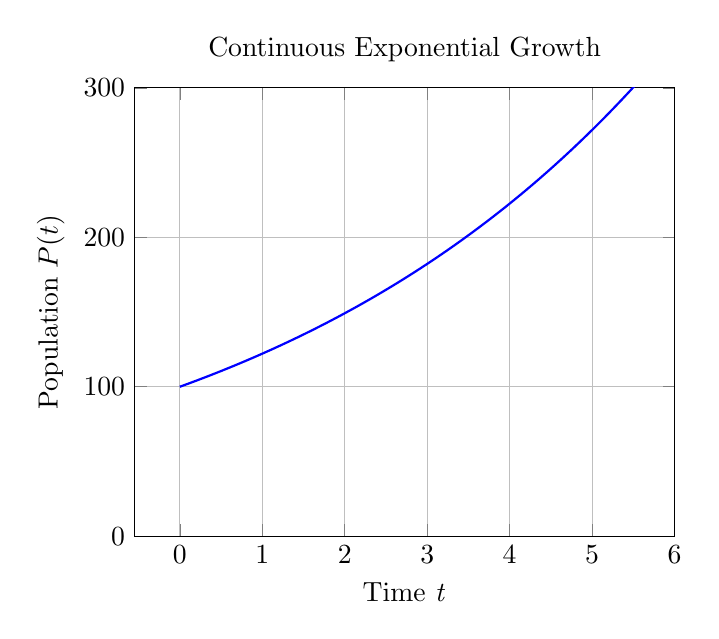
\begin{tikzpicture}
    \begin{axis}[
        xlabel={Time \emph{t}},
        ylabel={Population \(P(t)\)},
        title={Continuous Exponential Growth},
        domain=0:10,
        samples=100,
        ymin=0, ymax=300,
        grid=major,
    ]
    \addplot[blue, thick] {100*exp(0.2*x)};
    \end{axis}
    \end{tikzpicture}
\end{center}

\subsection{Logistic Growth}

Logistic growth occurs when a population grows rapidly at first and then slows as it approaches a maximum sustainable size (carrying capacity).

\subsubsection{Discrete Logistic Growth}

\[
    P_{n+1} = P_n + r \cdot P_n \cdot \left(1 - \frac{P_n}{K}\right)
\]

Where:

\begin{itemize}

  \item \(K\) is the carrying capacity

  \item \(r\) is the intrinsic growth rate

\end{itemize}

\textbf{Example:}
\vspace{\baselineskip}
  
With \(P_0 = 10\), \(r = 0.5\), \(K = 100\):

\[
    P_1 = 10 + 0.5 \cdot 10 \cdot \left(1 - \frac{10}{100}\right) = 10 + 0.5 \cdot 10 \cdot 0.9 = 10 + 4.5 = 14.5
\]

\begin{center}
    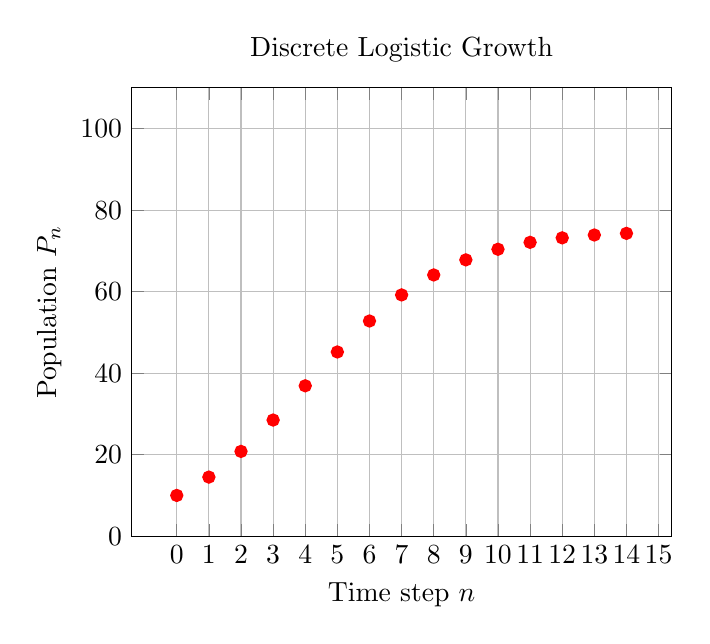
\begin{tikzpicture}
    \begin{axis}[
        xlabel={Time step \(n\)},
        ylabel={Population \(P_n\)},
        title={Discrete Logistic Growth},
        ytick={0,20,...,100},
        ymin=0, ymax=110,
        xtick={0,1,...,20},
        grid=major,
    ]
    \addplot+[only marks, mark=*, mark options={red}, thick] 
        table [row sep=\\] {
        x  y \\
        0  10 \\
        1  14.5 \\
        2  20.8 \\
        3  28.5 \\
        4  36.9 \\
        5  45.2 \\
        6  52.8 \\
        7  59.2 \\
        8  64.1 \\
        9  67.8 \\
        10 70.4 \\
        11 72.1 \\
        12 73.2 \\
        13 73.9 \\
        14 74.3 \\
        };
    \end{axis}
    \end{tikzpicture}
\end{center}

\subsubsection{Continuous Logistic Growth}

\[
    P(t) = \frac{K}{1 + \left( \frac{K - P_0}{P_0} \right)e^{-rt}}
\]

\textbf{Example:}
\vspace{\baselineskip}
  
With \(P_0 = 10\), \(K = 100\), and \(r = 0.5\), at \(t = 5\):

\[
    P(5) = \frac{100}{1 + \left( \frac{90}{10} \right)e^{-0.5 \cdot 5}} = \frac{100}{1 + 9e^{-2.5}} \approx \frac{100}{1.7387} \approx 57.52
\]

\begin{center}
    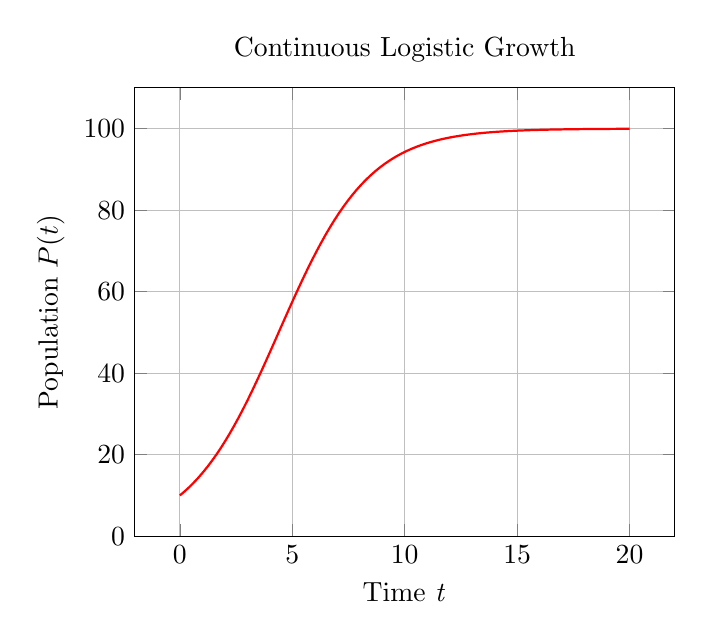
\begin{tikzpicture}
    \begin{axis}[
        xlabel={Time \emph{t}},
        ylabel={Population \(P(t)\)},
        title={Continuous Logistic Growth},
        domain=0:20,
        samples=100,
        ymin=0, ymax=110,
        grid=major,
    ]
    \addplot[red, thick] {100/(1 + (90/10)*exp(-0.5*x))};
    \end{axis}
    \end{tikzpicture}
\end{center}

\newpage
\section{Asymptotes}

An \emph{asymptote} of a curve is a line that the curve approaches but never touches as the input or output grows infinitely large in magnitude. There are three main types of asymptotes: vertical, horizontal, and oblique (slant). Each one describes a different long-term behavior of a function.

\subsection{Vertical Asymptotes}

A \emph{vertical asymptote} is a vertical line \(x = a\) where the function grows without bound as \(x\) approaches \(a\) from the left or right.

\[
\lim_{x \to a^-} f(x) = \pm \infty \quad \text{or} \quad \lim_{x \to a^+} f(x) = \pm \infty
\]

\subsubsection{How to Find Vertical Asymptotes}

\begin{enumerate}
    \item Find values of \(x\) that make the denominator of a rational function zero.
    \item Eliminate removable discontinuities (common factors).
    \item For each remaining zero in the denominator, check if the limit tends to infinity.
\end{enumerate}

\textbf{Example:}
\[
f(x) = \frac{1}{x - 2} \quad \Rightarrow \quad x = 2 \text{ is a vertical asymptote}
\]

\subsection{Horizontal Asymptotes}

A \emph{horizontal asymptote} is a horizontal line \(y = L\) that the function approaches as \(x\) tends to infinity or negative infinity:

\[
\lim_{x \to \pm\infty} f(x) = L
\]

\subsubsection{How to Find Horizontal Asymptotes (Rational Functions)}

\begin{enumerate}
    \item Compare the degrees of the numerator (\(n\)) and denominator (\(m\)):
    \begin{itemize}[label=\(-\)]
        \item If \(n < m\): Horizontal asymptote at \(y = 0\)
        \item If \(n = m\): Horizontal asymptote at \(y = \frac{\text{leading coefficient of numerator}}{\text{leading coefficient of denominator}}\)
        \item If \(n > m\): No horizontal asymptote (check for slant)
    \end{itemize}
\end{enumerate}

\textbf{Example:}
\[
f(x) = \frac{2x^2 + 3}{x^2 - 1} \quad \Rightarrow \quad y = \frac{2}{1} = 2 \text{ is the horizontal asymptote}
\]

\subsection{Oblique (Slant) Asymptotes}

An \emph{oblique or slant asymptote} occurs when the degree of the numerator is exactly one more than the degree of the denominator.

\[
\lim_{x \to \infty} [f(x) - (mx + b)] = 0
\]

\subsubsection{How to Find Oblique Asymptotes}

\begin{enumerate}
    \item Perform polynomial long division (or synthetic division) on the rational function.
    \item The quotient (ignoring the remainder) is the equation of the slant asymptote.
\end{enumerate}

\textbf{Example:}
\[
f(x) = \frac{x^2 + 1}{x - 1}
\]
Long division gives:
\[
\frac{x^2 + 1}{x - 1} = x + 1 + \frac{2}{x - 1}
\Rightarrow \text{Slant asymptote: } y = x + 1
\]

\subsection{Summary Table}

\begin{center}
\begin{tabular}{|l|l|l|}
\hline
\textbf{Type} & \textbf{Equation} & \textbf{Occurs When} \\
\hline
Vertical      & \(x = a\)           & Denominator \(\to 0\) (non-removable) \\
Horizontal    & \(y = L\)           & \(\lim_{x \to \pm \infty} f(x) = L\) \\
Oblique       & \(y = mx + b\)      & Degree numerator = degree denominator + 1 \\
\hline
\end{tabular}
\end{center}
\section{Sequences and Series}

A sequence is an ordered list of numbers, usually defined by a formula or a recurrence relation. It is one of the fundamental objects of study in mathematical analysis.

\subsection{Arithmetic Sequence}

An \textbf{arithmetic sequence} is a sequence where the difference between consecutive terms is constant.

\[
a_n = a_1 + (n - 1)d
\]

\begin{itemize}[label=\(-\)]
\item \(a_1\) is the first term
\item \(d\) is the common difference \(d = a_{n + 1} - a_{n}\)
\end{itemize}

\textbf{Example:}
\[
a_n = 3 + (n - 1) \cdot 2 = 2n + 1 \quad \text{(Odd numbers)}
\]

\subsection{Geometric Sequence}

A \textbf{geometric sequence} is a sequence where each term is obtained by multiplying the previous term by a fixed non-zero constant.

\[
a_n = a_1 \cdot r^{n-1}
\]

\begin{itemize}[label=\(-\)]
\item \(a_1\) is the first term
\item \(r\) is the common ratio \(r = \frac{a_{n + 1}}{a_n}\)
\end{itemize}

\textbf{Example:}
\[
a_n = 2 \cdot 3^{n-1} = 2, 6, 18, 54, \dots
\]

\subsection{Function Squence}

A \textbf{function sequence} is sequence composed of functions and its noted like:

\[
(f)_n \text{with } x^t := \{ f: D\to R | \ f \text{ is a funtion}\}
\]

\subsection{Convergence}

A sequence \((a_n)\) \textbf{converges} to a limit \(L\) if for every \(\varepsilon > 0\), there exists an integer \(n_0\) such that for all \(n \ge n_0\):

\[
|\forall \varepsilon > 0\ \exists n \in \mathbb{N}: \forall i \ge n\ |a_i - L| < \varepsilon
\]

In this case, we write:
\[
\lim_{n \to \infty} a_n = L
\]

\subsection{Cauchy Sequence}

A sequence \((a_n)\) is a \textbf{Cauchy sequence} if for every \(\varepsilon > 0\), there exists an integer \(n_0\) such that for all \(n, m \ge n_0\):

\[
\forall \varepsilon > 0\ \exists n,m \in \mathbb{N}: |a_n - a_m| < \varepsilon\ \text{with } n < m
\]

Every convergent sequence is a Cauchy sequence. In complete metric spaces (like \(\mathbb{R}\)), the converse also holds.

\textbf{Example: Convergence Exercise}

Let \(a_i = \frac{1}{i}\) and \(\varepsilon = 0.01\). We want to find \(i_0\) such that:

\[
\left|\frac{1}{n} - 0\right| < \varepsilon \implies \frac{1}{i} \le \frac{1}{n} < \varepsilon \rightarrow \frac{1}{\varepsilon} < n
\]
\[
\Rightarrow \frac{1}{i} < 0.01 \Rightarrow i > 100
\Rightarrow i_0 = 101
\]

\subsection{Definition of \texorpdfstring{\(\varepsilon\)}{ε}-Neighborhood}

The \textbf{\(\varepsilon\)-neighborhood} of a point \(a \in \mathbb{R}\) is the set:
\[
B_\varepsilon(a) = \{x \in \mathbb{R} \mid |x - a| < \varepsilon\}
\]
This is the open interval \((a - \varepsilon, a + \varepsilon)\).

\subsection{Supremum, Infimum, Maximum and Minimum}

The \textbf{supremum} of a set \(A \subseteq \mathbb{R}\) is the least upper bound: the smallest real number \(s\) such that \(a \le s\) for all \(a \in A\).

The \textbf{infimum} of a set \(A\) is the greatest lower bound: the largest number \(t\) such that \(a \ge t\) for all \(a \in A\).The \textbf{maximum} is the largest element in the set, if it exists.

The \textbf{minimum} is the smallest element in the set, if it exists.

\textbf{Example:} For \(A = (0,1)\):
\begin{itemize}[label=\(-\)]
\item \(\sup A = 1\) (not in \(A\))
\item \(\inf A = 0\) (not in \(A\))
\item \(\max A\) and \(\min A\) do not exist
\end{itemize}

\subsection{Limit and Accumulation Point}

\begin{itemize}[label=\(-\)]
\item A \textbf{limit} of a sequence \((a_n)\) is the value the terms get arbitrarily close to as \(n \to \infty\).
\item An \textbf{accumulation point} (or limit point) of a set \(A\) is a point \(x\) such that every neighborhood of \(x\) contains infinitely many points of \(A\).
\end{itemize}

\textbf{Example:} The sequence \(a_n = (-1)^n + \frac{1}{n}\) has two accumulation points: \(1\) and \(-1\).

\subsection{Monotonicity by Difference and Quotient}

\textbf{Monotonicity by Difference:}
\begin{itemize}[label=\(-\)]
\item If \(a_{n+1} - a_n \ge 0\) for all \(n\), then the sequence is non-decreasing.
\item If \(a_{n+1} - a_n \le 0\), it is non-increasing.
\end{itemize}

\textbf{Monotonicity by Quotient:} (Typically for positive sequences)
\begin{itemize}[label=\(-\)]
\item If \(\frac{a_{n+1}}{a_n} \ge 1\), then the sequence is non-decreasing.
\item If \(\frac{a_{n+1}}{a_n} \le 1\), it is non-increasing.
\end{itemize}

\subsection{Divergence (Definition)}

A sequence \textbf{diverges} if it does not converge. That is, there is no real number \(L\) such that:

\[
\lim_{n \to \infty} a_n = L
\]

\begin{itemize}[label=\(-\)]
\item A sequence can diverge to \(\infty\) or \(-\infty\)
\item A sequence can also oscillate without approaching any limit
\end{itemize}

\textbf{Example:} The sequence \(a_n = (-1)^n\) diverges since it oscillates between \(1\) and \(-1\).


\subsection{Subsequences and Their Properties}

A \textbf{subsequence} of a sequence \((a_n)\) is a sequence \((a_{n_k})\) where \((n_k)\) is a strictly increasing sequence of natural numbers.

\textbf{Properties:}
\begin{itemize}[label=\(-\)]
\item Every subsequence of a convergent sequence converges to the same limit.
\item A sequence converges if and only if all of its subsequences converge to the same limit.
\item A bounded sequence always has at least one convergent subsequence (Bolzano-Weierstraß theorem).
\end{itemize}

\subsection{Serie}

A \textbf{series} is the sum of the terms of a sequence:
\[
\sum_{n=1}^{\infty} a_n
\]
We define the partial sums \(S_n = \sum_{k=1}^n a_k\). If the sequence \((S_n)\) converges to a limit \(S\), then the series is said to converge:
\[
\sum_{n=1}^{\infty} a_n = S
\]

\subsection{Power Series}

A \textbf{power series} is a series of the form:
\[
\sum_{n=0}^{\infty} a_n (x - x_0)^n
\]
where \(x_0\) is the center of the expansion. Power series converge within a radius \(R\):
\[
R = \frac{1}{\limsup\limits_{n \to \infty} \sqrt[n]{|a_n|}}
\]

\subsection{Pointwise Convergence}

A sequence of functions \((f_n)\) converges \textbf{pointwise} to a function \(f\) on a set \(A\) if:
\[
\forall x \in A, \quad \lim_{n \to \infty} f_n(x) = f(x)
\]

Pointwise convergence does not preserve properties like continuity or differentiability.

\subsection{Uniform Convergence}

A sequence of functions \((f_n)\) converges \textbf{uniformly} to \(f\) on \(A\) if:
\[
\forall \varepsilon > 0, \exists n_0 \in \mathbb{N} \text{ such that } \forall n \ge n_0, \forall x \in A, \quad |f_n(x) - f(x)| < \varepsilon
\]

\textbf{Key Property:} Uniform convergence preserves continuity, integration, and differentiation under certain conditions.

\subsection{Cauchy Criterion for Series (Cauchy-Kriterium)}

A series \(\sum a_n\) converges if and only if for every \(\varepsilon > 0\) there exists \(n_0\) such that:
\[
\left| \sum_{k = m}^{n} a_k \right| < \varepsilon \quad \forall n > m \ge n_0
\]

\subsection{Interval Nesting and the Interval Nesting Theoreme}

Let \((I_n)\) be a sequence of closed intervals:
\[
I_n = [a_n, b_n] \quad \text{with } I_{n+1} \subseteq I_n, \text{ and } \lim_{n \to \infty} (b_n - a_n) = 0
\]
Then, the intersection contains exactly one point:
\[
\bigcap_{n=1}^{\infty} I_n = \{x\}
\]

This is useful in proving the existence of limits, roots, and fixed points.

\subsection{Weierstraß Approximation Theorem}

The \textbf{Weierstraß Approximation Theorem} states:

Every continuous function \(f: [a, b] \rightarrow \mathbb{R}\) can be uniformly approximated by a polynomial \(P(x)\), i.e., for every \(\varepsilon > 0\) there exists a polynomial \(P(x)\) such that:
\[
|f(x) - P(x)| < \varepsilon \quad \forall x \in [a, b]
\]

This theorem is foundational in numerical analysis and approximation theory.

\subsection{Zero Sequence}

A sequence \((a_n)\) is called a \textbf{null sequence} or \textbf{zero sequence} if:
\[
\lim_{n \to \infty} a_n = 0
\]
Every zero sequence is convergent (to 0), and plays an essential role in convergence proofs and epsilon-delta arguments.

\subsection{The Monotony Principle}

Every bounded monotonic sequence converges.

\begin{itemize}[label=\(-\)]
\item If \((a_n)\) is non-decreasing and bounded above, then \(\lim a_n\) exists and equals \(\sup \{a_n\}\).
\item If \((a_n)\) is non-increasing and bounded below, then \(\lim a_n = \inf \{a_n\}\).
\end{itemize}

To prove the converge of a sequence via this principle we follow the next steps

\begin{enumerate}
    \item Prove the Monotonicity by induction
    \item Calulate the limit
    \item Prove the boundness via induction
    \item Write the conclusion
\end{enumerate}

\textbf{Example: } \(a_{n + 1} = \sqrt{2a_n - 3} + 1\)

Lets assume that the series is decreasing or \(a_{n + 1} < a_{n}\)

\begin{align*}
    a_{n + 2} &< a{n + 1} \\
    \sqrt{2a_{n + 1} -3} + 1 &< \sqrt{2a_{n} - 3} + 1 \\
    \sqrt{2a_{n + 1} -3} &< \sqrt{2a_{n} - 3} \\
    2a_{n + 1} - 3 &< 2a_{n} - 3 \\
    a_{n + 1} &< a_{n}
\end{align*}
\QED

Now lets calculated the limit
\[
\lim_{n \rightarrow \infty} a_{n + 1} = \lim_{n \rightarrow \infty} \sqrt{2a_n - 3} + 1
\]

Because of the recursion we know that both \(a_{n + 1}\) and \(a_n\) have the same same value and we call it \(a\).
\[
a = \sqrt{2a -3} +1
\]
\[
a = 2
\]

We only have to prove the boundness now:

For \(n = 0\) we have \(a_1 = 4 > 2\) then lets assume that the \(a\) is never going bellow 2.

\[
a_{n + 1} = \sqrt{2a_n - 3} + 1 \ge \sqrt{2(2) - 3} + 1 = 2
\]

By setting \(a_n = 2\) we get the limit againg

\QED

\subsection{Operations on Sequences}

\subsubsection{Sum of Sequences}
The sum of two sequences \((a_n)\) and \((b_n)\) is a new sequence \((c_n)\) where each term \(c_n\) is the sum of the corresponding terms of \((a_n)\) and \((b_n)\):
\[
c_n = a_n + b_n, \quad \forall n \in \mathbb{N}.
\]
If \(\lim_{n \to \infty} a_n = A\) and \(\lim_{n \to \infty} b_n = B\), then the limit of the sum sequence is:
\[
\lim_{n \to \infty} (a_n + b_n) = A + B.
\]

\subsubsection{Multiplication of Sequences}
The product of two sequences \((a_n)\) and \((b_n)\) is a new sequence \((d_n)\) where each term \(d_n\) is the product of the corresponding terms of \((a_n)\) and \((b_n)\):
\[
d_n = a_n \cdot b_n, \quad \forall n \in \mathbb{N}.
\]
If \(\lim_{n \to \infty} a_n = A\) and \(\lim_{n \to \infty} b_n = B\), then the limit of the product sequence is:
\[
\lim_{n \to \infty} (a_n \cdot b_n) = A \cdot B.
\]

\subsubsection{Absolute Value of a Sequence}
The absolute value of a sequence \((a_n)\) is a new sequence \((e_n)\) where each term \(e_n\) is the absolute value of the corresponding term of \((a_n)\):
\[
e_n = |a_n|, \quad \forall n \in \mathbb{N}.
\]
If \(\lim_{n \to \infty} a_n = A\), then the limit of the absolute value sequence is:
\[
\lim_{n \to \infty} |a_n| = |A|.
\]

\subsubsection{Conjugate of a Complex Sequence}
If \((a_n)\) is a sequence of complex numbers, where \(a_n = x_n + i y_n\) with \(x_n, y_n \in \mathbb{R}\), then the conjugate of \((a_n)\) is a new sequence \((\overline{a_n})\) where each term \(\overline{a_n}\) is the complex conjugate of \(a_n\):
\[
\overline{a_n} = x_n - i y_n, \quad \forall n \in \mathbb{N}.
\]
If \(\lim_{n \to \infty} a_n = A = X + i Y\), then the limit of the conjugate sequence is:
\[
\lim_{n \to \infty} \overline{a_n} = \overline{A} = X - i Y.
\]

\subsubsection{Complex Limit (Real and Imaginary Parts)}
For a sequence of complex numbers \((a_n)\) where \(a_n = x_n + i y_n\), the limit of the sequence \(\lim_{n \to \infty} a_n = A = X + i Y\) exists if and only if the limits of the real part sequence \((x_n)\) and the imaginary part sequence \((y_n)\) exist individually:
\[
\lim_{n \to \infty} a_n = A \iff \left( \lim_{n \to \infty} \text{Re}(a_n) = \text{Re}(A) = X \quad \text{and} \quad \lim_{n \to \infty} \text{Im}(a_n) = \text{Im}(A) = Y \right).
\]
This means we can analyze the convergence of a complex sequence by examining the convergence of its real and imaginary parts separately.

\subsubsection{Asymptotic Equality}
Two sequences \((a_n)_{n \in \mathbb{N}}\) and \((b_n)_{n \in \mathbb{N}}\) are said to be asymptotically equal, denoted by \(a_n \sim b_n\), if
\[
\lim_{n \to \infty} \frac{a_n}{b_n} = 1,
\]
provided that \(b_n \neq 0\) for all sufficiently large \(n\). Asymptotic equality implies that the sequences behave similarly as \(n\) approaches infinity.

\newpage

\newpage
\section{Limits}

Limits are a foundational concept in calculus and analysis. They describe the behavior of 
functions and sequences as the input approaches a particular value or infinity.

\subsection{Definition of the Limit}

Let \(f\) be a function defined near a point \(a\). We say:

\[
    \lim_{x \to a} f(x) = L
\]

if for every \(\varepsilon > 0\), there exists a \(\delta > 0\) such that:

\[
    0 < |x - a| < \delta \Rightarrow |f(x) - L| < \varepsilon
\]

This is the precise \emph{\(\varepsilon\)-\(\delta\) definition} of a limit.

\subsection{Limit Calculation Rules}

\emph{Sum Rule:} \(\displaystyle \lim_{x \to a} (f(x) + g(x)) = \lim_{x \to a} f(x) + \lim_{x \to a} g(x)\)

\emph{Difference Rule:} \(\displaystyle \lim_{x \to a} (f(x) - g(x)) = \lim_{x \to a} f(x) - \lim_{x \to a} g(x)\)

\emph{Product Rule:} \(\displaystyle \lim_{x \to a} (f(x)g(x)) = \lim_{x \to a} f(x) \cdot \lim_{x \to a} g(x)\)

\emph{Quotient Rule:} \(\displaystyle \lim_{x \to a} \frac{f(x)}{g(x)} = \frac{\lim f(x)}{\lim g(x)}\) if \(\lim g(x) \ne 0\)

\emph{Power Rule:} \(\displaystyle \lim_{x \to a} {f(x)}^n = {(\lim_{x \to a} f(x))}^n\)

\emph{Root Rule:} \(\displaystyle \lim_{x \to a} \sqrt[n]{f(x)} = \sqrt[n]{\lim_{x \to a} f(x)}\) (when defined)

\subsection{Limits at Infinity}

\[
    \lim_{x \to \infty} f(x) = L \quad \text{means that } f(x) \text{ approaches } L \text{ as } x \to \infty
\]

\[
    \lim_{x \to \infty} \frac{1}{x} = 0, \quad \lim_{x \to \infty} e^x = \infty, \quad \lim_{x \to \infty} \frac{1}{x^2} = 0
\]

\subsection{Indeterminate Forms}

Indeterminate forms arise in limits when the expression does not directly imply a limit value:

\[
    \frac{0}{0}, \quad \frac{\infty}{\infty}, \quad 0 \cdot \infty, \quad \infty - \infty, \quad 1^\infty, \quad \infty^0, \quad 0^0
\]

\subsection{Limit of a Composite Function}

If \(\displaystyle \lim_{x \to a} f(x) = L\) and \(\displaystyle \lim_{x \to L} g(x) = g(L)\) 
(i.e., \(g\) is continuous at \(L\)), then:

\[
    \lim_{x \to a} g(f(x)) = g\left(\lim_{x \to a} f(x)\right)
\]

\subsection{Right and Left Limits}

\[
    \lim_{x \to a^-} f(x) = L_-, \quad \lim_{x \to a^+} f(x) = L_+
\]

The two-sided limit \(\displaystyle \lim_{x \to a} f(x)\) exists if and only if \(L_- = L_+\).

\subsection{L’Hôpital’s Rule}

If \(\displaystyle \lim_{x \to a} f(x) = \lim_{x \to a} g(x) = 0\) or \(\pm\infty\), and \(\displaystyle \lim_{x \to a} \frac{f'(x)}{g'(x)}\) exists, then:

\[
    \lim_{x \to a} \frac{f(x)}{g(x)} = \lim_{x \to a} \frac{f'(x)}{g'(x)}
\]

This rule is used to resolve indeterminate forms \(\frac{0}{0}\) and \(\frac{\infty}{\infty}\).

\subsection{Limit of a fraction}

For expressions like:

\[
    \lim_{n \to \infty} {\left( \frac{a}{b} \right)}^n
\]

\begin{itemize}

    \item If \(\frac{a}{b} < 1\): limit is \(0\)

    \item If \(\frac{a}{b} > 1\): limit diverges to \(\infty\)

\end{itemize}

\subsection{Limit of a Recursive Sequence}

Let \((a_n)\) be defined recursively:

\[
    a_{n+1} = f(a_n)
\]

If \((a_n)\) converges to \(L\) and \(f\) is continuous, then:

\[
    \lim_{n \to \infty} a_n = L \Rightarrow L = f(L)
\]

This is used to find fixed points of recursive definitions.

\subsection{Important Limits}

\begin{itemize}

    \item \(\displaystyle \lim_{x \to 0} \frac{\sin x}{x} = 1\)

    \item \(\displaystyle \lim_{x \to 0} \frac{1 - \cos x}{x^2} = \frac{1}{2}\)

    \item \(\displaystyle \lim_{x \to 0} \frac{\ln(1 + x)}{x} = 1\)

    \item \(\displaystyle \lim_{x \to 0} \frac{e^x - 1}{x} = 1\)

    \item \(\displaystyle \lim_{n \to \infty} \frac{n!}{n^n} = 0\)

    \item \(\displaystyle \lim_{n \to \infty} \sqrt[n]{a} = 1\) (for \(a > 0\))

    \item \(\displaystyle \lim_{x \to 0} \frac{1}{\cos x} = 1\)

\end{itemize}

\subsection{Squeeze Theorem (Sandwich Theorem)}

If \(g(x) \le f(x) \le h(x)\) near \(a\), and:

\[
    \lim_{x \to a} g(x) = \lim_{x \to a} h(x) = L
    \Rightarrow \lim_{x \to a} f(x) = L
\]

\textbf{Example:}

\[
    \lim_{x \to 0} x^2 \cos\left( \frac{1}{x} \right) = 0
\]

\subsection{The Number \texorpdfstring{\(e\)}{e} as a Limit}

The number \(e\) is defined as:

\[
    e = \lim_{n \to \infty} {\left(1 + \frac{1}{n} \right)}^n
\]

More generally:

\[
    \lim_{n \to \infty} {\left(1 + \frac{a}{bn} \right)}^n = e^{a/b}
\]

\textbf{Example of a limit using e}

\[
    \lim_{x \to \infty}{\left(\frac{x^2 + 1}{x^2 +2}\right)}^{x^2}
\]

\[
    \lim_{x \to \infty} {\left({\left(\frac{x^2 + 1}{x^2 +2}\right)}^{x}\right)}^x
\]

\[
    \lim_{x \to \infty} {\left({\left(\frac{1 + \frac{1}{x^2}}{1 + \frac{2}{x^2}}\right)}^{x}\right)}^x
\]

\[
    \lim_{x \to \infty} {\left(\frac{e}{e^2}\right)}^x = {\left(\frac{1}{e}\right)}^x = 0
\]

\subsection{Limits of \texorpdfstring{\(\arctan\)}{arctan}}

\begin{itemize}

    \item \(\lim_{x \to \infty} \arctan x = \frac{\pi}{2}\)

    \item \(\lim_{x \to -\infty} \arctan x = -\frac{\pi}{2}\)

    \item \(\arctan x\) is continuous and differentiable everywhere, with a horizontal asymptote at 
    \(y = \pm \frac{\pi}{2}\)

\end{itemize}

\subsection{Bolzano-Weierstraß Theorem}

Every bounded, convergent sequence in \(\Complex\) has a convergent subsequence.
More precisely the sequence \(a\) has biggest and smallest accumulation point \(h^*\) and \(h_*\)

\[
    \forall \varepsilon > 0 : h_* - \varepsilon < a_n < h^{*} + \varepsilon \text{ for all-most all } 
    b \in \Naturals
\]

\[
    h^* := \lim_{n \to \infty} \sup a_n
\]

\[
    h_* := \lim_{n \to \infty} \inf a_n
\]

\subsection{Uniqueness of the Limit}

Let \( f: D \subset \Reals \to \Reals \), and suppose \(a\) is a limit point of \( D \). Then:
If \( \lim_{x \to a} f(x) = L_1 \) and \( \lim_{x \to a} f(x) = L_2 \), then \( L_1 = L_2 \).

In other words, a function can have at most one limit at a given point. This is the \emph{uniqueness of limits}.

\textbf{Proof (by contradiction)}

Assume \( L_1 \ne L_2 \), and let \( \varepsilon = \frac{|L_1 - L_2|}{3} > 0 \).

\begin{itemize}

    \item Since \( \lim_{x \to a} f(x) = L_1 \), there exists \( \delta_1 > 0 \) such that for all \( x \in D \), \( 0 < |x - a| < \delta_1 \) implies:

    \[
        |f(x) - L_1| < \varepsilon
    \]
    
    \item Since \( \lim_{x \to a} f(x) = L_2 \), there exists \( \delta_2 > 0 \) such that for all \( x \in D \), \( 0 < |x - a| < \delta_2 \) implies:

    \[
        |f(x) - L_2| < \varepsilon
    \]

\end{itemize}

Let \( \delta = \min(\delta_1, \delta_2) \), and choose \( x \in D \) such that \( 0 < |x - a| < \delta \).

Then:

\[
    |f(x) - L_1| < \varepsilon, \quad |f(x) - L_2| < \varepsilon
\]

Using the triangle inequality:

\[
    |L_1 - L_2| = |L_1 - f(x) + f(x) - L_2| \le |f(x) - L_1| + |f(x) - L_2| < \varepsilon + \varepsilon = 2\varepsilon
\]

But we chose \( \varepsilon = \frac{|L_1 - L_2|}{3} \), so:

\[
    |L_1 - L_2| < \frac{2}{3}|L_1 - L_2| \Rightarrow \frac{1}{3}|L_1 - L_2| < 0
\]

Which is a contradiction since absolute values are always non-negative.

\textbf{Conclusion:} Our assumption was false. Hence, \( L_1 = L_2 \). The limit is unique.

\QED

\subsection{Every Convergent Sequence is a Cauchy Sequence}

Let \( (a_n) \) be a sequence in \( \Reals \). We say:

If \( (a_n) \) converges, then it is a Cauchy sequence.

A sequence \( (a_n) \) is a \emph{Cauchy sequence} if:

\[
    \forall \varepsilon > 0, \ \exists N \in \Naturals \text{ such that } \forall n, m \ge N, \quad |a_n - a_m| < \varepsilon
\]

\textbf{Proof:}

Assume \( \lim_{n \to \infty} a_n = L \). Then:

\begin{itemize}

    \item For every \( \varepsilon > 0 \), there exists \( N \in \Naturals \) such that:

    \[
        \forall n \ge N, \quad |a_n - L| < \frac{\varepsilon}{2}
    \]

    \item Now, for any \( n, m \ge N \), use the triangle inequality:

    \[
        |a_n - a_m| = |a_n - L + L - a_m| \le |a_n - L| + |a_m - L| < \frac{\varepsilon}{2} + \frac{\varepsilon}{2} = \varepsilon
    \]

\end{itemize}

\textbf{Conclusion:}  

\(|a_n - a_m| < \varepsilon \text{ for all } n, m \ge N \Rightarrow (a_n) \text{ is Cauchy}\)

This completes the proof that every convergent sequence is Cauchy.

\QED
\newpage
\section{Convergence Radius}

Consider a power series of the form

\[
    f(x) = \sum_{n=0}^{\infty} c_n {(x - a)}^n,
\]

where \(c_n\) are the coefficients, \(x\) is the variable, and \(a\) is the center of the series. 
The radius of convergence, denoted by \(R\), is a non-negative real number (or \(\infty\)) 
such that the series converges if \(|x - a| < R\) and diverges if \(|x - a| > R\). In other words, 
the interval of convergence is \((a - R, a + R)\), possibly including one or both endpoints.

\[
    R = \frac{1}{\limsup_{n \to \infty} \sqrt[n]{|a_n|}}
\]

or 

\[
    R = \limsup_{n \to \infty} \frac{a_n}{ a_{n + 1}}
\]

\subsection{Test of the Borders}

When the absolute value of the difference between \(x\) and \(a\) is equal to the radius of convergence 
(i.e., \(|x - a| = R\)), the convergence of the power series must be checked separately. This involves 
substituting the values \(x = a \pm R\) into the series and determining whether the resulting series 
converges or diverges using other convergence tests (e.g., the comparison test, ratio test, alternating 
series test).

\subsection{Approximating the Error}

When a power series is used to approximate a function, it is often necessary to estimate the error in the 
approximation. If the power series converges, the error can be made arbitrarily small by including a 
sufficient number of terms. For an alternating series that satisfies the conditions of the Alternating 
Series Test, the error in approximating the sum by the first \(n\) terms is bounded by the absolute value 
of the \((n+1)\)-th term:

\[
    \left| \sum_{k=0}^{\infty} c_k {(x - a)}^k - \sum_{k=0}^{n} c_k {(x - a)}^k \right| \leq |c_{n+1} {(x - a)}^{n+1}|.
\]

For other power series, techniques such as Taylor's Theorem with remainder can be used to estimate the error.

\subsection{Complete Example}

Find the convergence radius of 

\[
    \sum_{n = 1}^{\infty} \frac{x^n}{n2^n} 
\]

at \(x = 0\).

\textbf{Step 1: Extract the sequence \(a_n\)}

The general form is 

\[
    \sum_{0}^{\infty} a_n (x - x_0)^n 
\]

in our case

\[
    = \sum_{n = 1}^{\infty} x^n \frac{1}{n2^n}
\]

with \(\frac{1}{n2^n}\) as \(a_n\).

\textbf{Step 2: Compute the radius}

\begin{align*}
     R &= \frac{1}{\limsup_{n \to \infty} \sqrt[n]{\frac{1}{n2^n}}} \\
      &= \frac{1}{\limsup_{n \to \infty}\frac{\sqrt[n]{1}}{\sqrt[n]{n} \sqrt[n]{2^n}}} \\
      &= \frac{1}{\frac{1}{2}} = 2
\end{align*}

\textbf{Step 3: Check Borders}

The borders to check are \( 0 - 2 \) to \( 0 + 2 \).

For -2:

\[
    \sum_{n = 1}^{\infty} \frac{(-2)^n}{n2^n} = \sum_{n = 1}^{\infty} \frac{(-1)^n (2)^n}{n2^n} 
    = \sum_{n = 1}^{\infty} \frac{(-1)^n}{n} 
\]

by Leibniz, it converges.

For 2:

\[
    \sum_{n = 1}^{\infty} \frac{(2)^n}{n2^n} = \sum_{n = 1}^{\infty} \frac{1}{n}
\]

This is the harmonic series therefore it diverges.

\textbf{Step 4: Write the interval}

The final interval of convergence is \([-2, 2)\).












\newpage
\section{Calculating Series Values}

\subsection{Telescoping Sums and Partial Fraction Decomposition}
Telescoping sums are series where most of the terms cancel out, leaving only a few terms. Partial fraction decomposition is a technique used to rewrite rational functions as a sum of simpler fractions, which can often lead to telescoping sums.

\textbf{Example: \(\sum_{k=1}^{\infty} \frac{1}{4k^2 - 1}\)}

Consider the infinite series
\[
S = \sum_{k=1}^{\infty} \frac{1}{4k^2 - 1}.
\]
We can decompose the fraction using partial fraction decomposition:
\[
\frac{1}{4k^2 - 1} = \frac{1}{(2k - 1)(2k + 1)} = \frac{A}{2k - 1} + \frac{B}{2k + 1}.
\]
Multiplying both sides by \((2k - 1)(2k + 1)\) gives
\[
1 = A(2k + 1) + B(2k - 1).
\]
To solve for \(A\) and \(B\), we can use the following values of \(k\):
\begin{itemize}[label=\(-\)]
    \item For \(k = \frac{1}{2}\): \(1 = A(1 + 1) + B(0) \implies A = \frac{1}{2}\).
    \item For \(k = -\frac{1}{2}\): \(1 = A(0) + B(-1 - 1) \implies B = -\frac{1}{2}\).
\end{itemize}
Thus, we have
\[
\frac{1}{4k^2 - 1} = \frac{1}{2} \left( \frac{1}{2k - 1} - \frac{1}{2k + 1} \right).
\]
Now we can write the series as a telescoping sum:
\[
S = \frac{1}{2} \sum_{k=1}^{\infty} \left( \frac{1}{2k - 1} - \frac{1}{2k + 1} \right).
\]
Let \(S_n\) be the \(n\)-th partial sum:
\begin{align*}
S_n &= \frac{1}{2} \left[ \left( \frac{1}{1} - \frac{1}{3} \right) + \left( \frac{1}{3} - \frac{1}{5} \right) + \left( \frac{1}{5} - \frac{1}{7} \right) + \cdots + \left( \frac{1}{2n - 1} - \frac{1}{2n + 1} \right) \right] \\
&= \frac{1}{2} \left[ 1 - \frac{1}{2n + 1} \right].
\end{align*}
Taking the limit as \(n\) approaches infinity, we get
\[
S = \lim_{n \to \infty} S_n = \lim_{n \to \infty} \frac{1}{2} \left( 1 - \frac{1}{2n + 1} \right) = \frac{1}{2} (1 - 0) = \frac{1}{2}.
\]
Therefore, the value of the series is \(\frac{1}{2}\).

\section{Transforming Functions into Power Series}

Many functions can be represented as power series, which is useful for various applications in calculus and analysis. This section discusses some common techniques for transforming functions into power series.

\subsection{Common Cases}
Here are some common cases where functions can be easily transformed into power series:

\subsubsection{\(\frac{1}{1 - x}\)}
The function \(\frac{1}{1 - x}\) has the well-known geometric series representation:
\[
\frac{1}{1 - x} = \sum_{n=0}^{\infty} x^n, \quad |x| < 1.
\]

\subsubsection{\(\frac{1}{1 - (x - x_0)^n}\)}
A slight generalization is:
\[
\frac{1}{1 - (x - x_0)^n} = \sum_{k=0}^{\infty} (x - x_0)^{nk}, \quad |x - x_0| < 1.
\]

\subsubsection{\(\frac{1}{1 - d(x - x_0)^n}\)}
For a constant \(d\):
\[
\frac{1}{1 - d(x - x_0)^n} = \sum_{k=0}^{\infty} d^k (x - x_0)^{nk}, \quad |d(x - x_0)^n| < 1.
\]

\subsection{Example: \(\frac{x + 1}{3 - x}\)}
Let's find the power series representation of the function \(f(x) = \frac{x + 1}{3 - x}\).

\subsubsection{Partial Fractions}
First, we perform partial fraction decomposition. We can rewrite the function as:
\[
\frac{x + 1}{3 - x} = \frac{-(3 - x) + 4}{3 - x} = -1 + \frac{4}{3 - x}.
\]

\subsubsection{Manipulating the Expression}
Now, we manipulate the fraction to fit the form \(\frac{1}{1 - u}\):
\[
\frac{4}{3 - x} = \frac{4}{3(1 - \frac{x}{3})} = \frac{4}{3} \cdot \frac{1}{1 - \frac{x}{3}}.
\]

\subsubsection{Power Series Representation}
Using the geometric series formula, we have
\[
\frac{1}{1 - \frac{x}{3}} = \sum_{n=0}^{\infty} \left( \frac{x}{3} \right)^n, \quad \left| \frac{x}{3} \right| < 1.
\]
Thus,
\begin{align*}
\frac{x + 1}{3 - x} &= -1 + \frac{4}{3} \sum_{n=0}^{\infty} \left( \frac{x}{3} \right)^n \\
&= -1 + \frac{4}{3} \sum_{n=0}^{\infty} \frac{x^n}{3^n} \\
&= -1 + \sum_{n=0}^{\infty} \frac{4}{3^{n+1}} x^n, \quad |x| < 3.
\end{align*}
Therefore, the power series representation of the function is
\[
\frac{x + 1}{3 - x} = -1 + \sum_{n=0}^{\infty} \frac{4}{3^{n+1}} x^n, \quad |x| < 3.
\]

\newpage
\newpage
\section{Continuity}

Continuity describes functions whose values change smoothly, without abrupt jumps or breaks. 
This concept is fundamental in calculus, analysis, and fixed point theory.

\subsection{Definition of Continuity at a Point}

A function \(f\) is \emph{continuous} at a point \(x_0\) if:

\[
    \forall \varepsilon > 0, \exists \delta > 0 \text{ such that } |x - x_0| < \delta \Rightarrow |f(x) - f(x_0)| < \varepsilon
\]

Equivalently,

\[
    \lim_{x \to x_0} f(x) = f(x_0)
\]

\textbf{Example:} 

\(\varepsilon \delta\) Exercise for \(f(x) = \frac{1}{x}\) at \(x_0 > 0\)

We want to find \(\delta\) such that:

\[
    |x - x_0| < \delta \Rightarrow \left|\frac{1}{x} - \frac{1}{x_0}\right| < \varepsilon
\]

Start by rewriting:
\[
    \left|\frac{1}{x} - \frac{1}{x_0}\right| = \left|\frac{x_0 - x}{xx_0}\right| = \frac{|x - x_0|}{|x||x_0|}
\]

Assume:

\[
    x \in \left[\frac{x_0}{2}, \frac{3x_0}{2}\right] \Rightarrow |x| \ge \frac{x_0}{2}
\]

Then:

\[
    \left|\frac{1}{x} - \frac{1}{x_0}\right| \le \frac{|x - x_0|}{\frac{x_0}{2} \cdot x_0} = \frac{2}{x_0^2} |x - x_0|
\]

Choose:

\[
    \delta = \min\left\{\frac{x_0}{2}, \frac{x_0^2 \varepsilon}{2} \right\}
\]

\subsection{Rules of Continuity}

Let \(f\) and \(g\) be continuous at \(x_0\):

\begin{itemize}
    
    \item \(f + g\), \(f - g\), \(f \cdot g\) are continuous at \(x_0\)
    
    \item \(\frac{f}{g}\) is continuous at \(x_0\) if \(g(x_0) \ne 0\)
    
    \item Compositions: if \(g\) is continuous at \(x_0\), and \(f\) is continuous at \(g(x_0)\), 
    then \(f \circ g\) is continuous at \(x_0\)

\end{itemize}

\subsection{Lipschitz Continuity}

A function \(f: D \subset \Reals \to \Reals\) is \emph{Lipschitz continuous} if:

\[
    \exists L > 0 \text{ such that } |f(x) - f(y)| \le L |x - y| \quad \forall x, y \in D
\]

\begin{itemize}

    \item Every Lipschitz continuous function is uniformly continuous.

    \item The smallest such \(L\) is called the \emph{Lipschitz constant}.

\end{itemize}

\subsection{Banach Fixed Point Theorem}

Let \((X, d)\) be a complete metric space, and \(f: X \to X\) a \emph{contraction mapping}, i.e.,

\[
    \exists L < 1 \text{ such that } d(f(x), f(y)) \le L \cdot d(x, y)
\]

Then:

\begin{itemize}

    \item \(f\) has a unique fixed point \(x^* \in X\), such that \(f(x^*) = x^*\)

    \item Iterating \(x_{n+1} = f(x_n)\) converges to \(x^*\)

\end{itemize}

\emph{Interpretation and Meaning}

The Banach Fixed Point Theorem ensures:

\begin{itemize}

    \item Existence and uniqueness of solutions (fixed points)

    \item Convergence of approximation by iteration

    \item Powerful tool in numerical methods and differential equations

\end{itemize}

\subsubsection{A Priori and A Posteriori Approximations}

\emph{A priori estimate:}

\[
    |x_n - x^*| \le \frac{L^n}{1 - L} |x_1 - x_0|
\]

\emph{A posteriori estimate:}

\[
    |x_n - x^*| \le \frac{L}{1 - L} |x_n - x_{n-1}|
\]

\subsubsection{Steps for a Fixed Point Exercise}

Given \(f: [a, b] \to [a, b]\), to prove existence and convergence:

\begin{enumerate}

    \item \textbf{Show monotonicity:} \(f\) is increasing or decreasing.

    \item \textbf{Check interval preservation:} \(f([a, b]) \subseteq [a, b]\)

    \item \textbf{Check Lipschitz continuity:} Find \(L < 1\)

    \item \textbf{Fixed point iteration:} Choose \(x_0\), compute \(x_{n+1} = f(x_n)\)

    \item \textbf{Apply a priori or a posteriori bound}

\end{enumerate}

\textbf{Example: \(f(x) = \frac{1}{x} + 3\) on \([2, 5]\)}

\begin{itemize}

    \item \emph{Domain check:} \(x \in [2, 5] \Rightarrow \frac{1}{x} \in [0.2, 0.5] \Rightarrow f(x) \in [3.2, 3.5] \subset [2, 5]\)

    \item \emph{Lipschitz constant:}

        \[
            f'(x) = -\frac{1}{x^2} \Rightarrow |f'(x)| \le \frac{1}{2^2} = \frac{1}{4} < 1
            \Rightarrow \text{Lipschitz with } L = \frac{1}{4}
        \]

    \item \emph{Contraction verified:} By derivative bound

    \item \emph{Fixed point iteration:}

        \[
            x_0 = 3, \quad x_1 = f(3) = \frac{1}{3} + 3 = \frac{10}{3}, \quad x_2 = f(x_1), \dots
        \]

    \item \emph{Use approximation bounds:}

        \[
            |x_n - x^*| \le \frac{L^n}{1 - L} |x_1 - x_0|
        \]
\end{itemize}
\newpage
\section{Differentiation}

Differentiation is a core concept in calculus. It describes the rate at which a quantity changes and provides tools for analyzing and modeling change in real-world phenomena.

\subsection{Definition of the Derivative}

The derivative of a function \(f\) at a point \(x\) is defined as the limit:
\[
f'(x) = \lim_{h \to 0} \frac{f(x + h) - f(x)}{h}
\]

or

\[f'(x) = \lim_{h \to a}\frac{f(x) - f(a)}{x - a}\]
provided this limit exists.

Geometrically, \(f'(a)\) is the slope of the tangent line to the graph of \(f\) at \(x = a\).

\subsection{Derivative Rules}

\emph{Power Rule:}
\[
\frac{d}{dx} x^n = nx^{n - 1}, \quad \text{for } n \in \mathbb{R}
\]
\emph{Constant Rule:}
\[
\frac{d}{dx} c = 0, \quad \text{for constant } c
\]
\emph{Constant Multiple Rule:}
\[
\frac{d}{dx} [c \cdot f(x)] = c \cdot f'(x)
\]
\emph{Sum and Difference Rule:}
\[
\frac{d}{dx} [f(x) \pm g(x)] = f'(x) \pm g'(x)
\]
\emph{Product Rule:}
\[
\frac{d}{dx} [f(x)g(x)] = f'(x)g(x) + f(x)g'(x)
\]
\emph{Quotient Rule:}
\[
\frac{d}{dx} \left( \frac{f(x)}{g(x)} \right) = \frac{f'(x)g(x) - f(x)g'(x)}{[g(x)]^2}
\]
\emph{Chain Rule:}
\[
\frac{d}{dx} f(g(x)) = f'(g(x)) \cdot g'(x)
\]

\subsection{Extrema and Critical Points Test}

A function \(f\) has a critical point at \(x = c\) if:
\[
f'(c) = 0 \quad \text{or} \quad f'(c) \text{ does not exist}
\]

To determine the nature of the critical point:
\begin{itemize}[label=\(-\)]
\item \emph{First Derivative Test:} Check sign changes of \(f'\) around \(c\)
\item \emph{Second Derivative Test:}
\[
f''(c) > 0 \Rightarrow \text{local minimum} \\
f''(c) < 0 \Rightarrow \text{local maximum}
\]
\end{itemize}

\subsection{Trigonometric Derivatives}

\begin{align*}
\frac{d}{dx} \sin x &= \cos x \\
\frac{d}{dx} \cos x &= -\sin x \\
\frac{d}{dx} \tan x &= \sec^2 x \\
\frac{d}{dx} \cot x &= -\csc^2 x \\
\frac{d}{dx} \sec x &= \sec x \tan x \\
\frac{d}{dx} \csc x &= -\csc x \cot x
\end{align*}

\subsection{Derivatives of Inverse Trigonometric Functions}

\begin{align*}
\frac{d}{dx} \arcsin x &= \frac{1}{\sqrt{1 - x^2}} \\
\frac{d}{dx} \arccos x &= -\frac{1}{\sqrt{1 - x^2}} \\
\frac{d}{dx} \arctan x &= \frac{1}{1 + x^2} \\
\frac{d}{dx} arcot x &= -\frac{1}{1 + x^2} \\
\frac{d}{dx} arcsec x &= \frac{1}{|x|\sqrt{x^2 - 1}} \\
\frac{d}{dx} arccsc x &= -\frac{1}{|x|\sqrt{x^2 - 1}}
\end{align*}

\subsection{The Differential}

The differential \(dy\) of a function \(y = f(x)\) is defined as:
\[
dy = f'(x) \, dx
\]

This linear approximation estimates the change in \(y\) for a small change in \(x\).

\subsection{The Secant Equation and Graphical Meaning}

The \emph{secant line} through points \((x_0, f(x_0))\) and \((x_0 + h, f(x_0 + h))\) has slope:
\[
\frac{f(x_0 + h) - f(x_0)}{h}
\]

As \(h \to 0\), the secant line approaches the tangent line. Graphically, this means:
\[
\lim_{h \to 0} \text{slope of secant} = \text{slope of tangent} = f'(x) = \Delta_h
\]

The secant line equation is given by:

\[
L(x) = f(x) + \Delta_h f(x_0)(x - x_0)
\]

\subsection{Optimization via the Derivative}

To find local or global extrema:
\begin{enumerate}
    \item Compute \(f'(x)\)
    \item Solve \(f'(x) = 0\) to find critical points
    \item Use the first or second derivative test to classify
    \item Evaluate endpoints if optimizing over a closed interval
\end{enumerate}

\textbf{Example:} Maximize area \(A = x(10 - 2x)\)

\[
A = 10x - 2x^2, \quad A' = 10 - 4x, \quad A' = 0 \Rightarrow x = 2.5
\]

\subsection{Power Rule Derivation}

We derive the power rule:
\[
\frac{d}{dx} x^n = nx^{n - 1}
\]
for \(n \in \mathbb{N}\) using the limit definition:
\[
\frac{d}{dx} x^n = \lim_{h \to 0} \frac{(x + h)^n - x^n}{h}
\]
Use the Binomial Theorem:
\[
(x + h)^n = x^n + nx^{n-1}h + \cdots + h^n
\Rightarrow \text{Only the linear term survives after dividing by } h
\]

\subsection{Implicit Differentiation}

Given:
\[
9x^2 + 4y^2 = 25
\]
Differentiate both sides implicitly:
\[
18x + 8y \frac{dy}{dx} = 0
\Rightarrow \frac{dy}{dx} = -\frac{18x}{8y} = -\frac{9x}{4y}
\]

This method is used when \(y\) is not isolated and is defined implicitly.

\newpage
\section{Integration}

Integration is the reverse process of differentiation and is used to calculate areas, volumes, 
accumulated change, and more.

\subsection{Definition (Riemann Integral)}

Let \(f: [a, b] \to \Reals\) be a bounded function. We define the \emph{definite integral} as:

\[
    \int_a^b f(x)\,dx = \lim_{\|P\| \to 0} \sum_{i=1}^n f(\xi_i)\Delta x_i
\]

Where \(P = \{x_0, \dots, x_n\}\) is a partition, \(\xi_i \in [x_{i-1}, x_i]\), and 
\(\Delta x_i = x_i - x_{i-1}\).

\subsection{Upper and Lower Sums}

Let \(f\) be bounded on \([a, b]\) and \(P\) a partition:

\[
    \underline{S}(f, P) = \sum_{i=1}^n m_i \Delta x_i, \quad
    \overline{S}(f, P) = \sum_{i=1}^n M_i \Delta x_i
\]

with:

\[
    m_i = \inf_{x \in [x_{i-1}, x_i]} f(x), \quad
    M_i = \sup_{x \in [x_{i-1}, x_i]} f(x)
\]

If \(\sup \underline{S} = \inf \overline{S}\), then \(f\) is Riemann integrable.

\subsection{Concrete and Non-Concrete Integrals}

\begin{itemize}

    \item \emph{Concrete:} Can be explicitly evaluated with anti-derivatives.

    \item \emph{Non-concrete:} Cannot be integrated in elementary terms (e.g., \(\int e^{-x^2} dx\)).

\end{itemize}

\subsection{Rules of Integration}

\begin{itemize}

    \item \(\int 0\,dx = C\)

    \item \(\int c\,dx = cx\)

    \item \(\int x^n\,dx = \frac{x^{n+1}}{n+1} + C \quad (n \ne -1)\)

    \item \(\int \frac{1}{x}\,dx = \ln|x| + C\)

    \item \(\int e^x\,dx = e^x + C\)

    \item \(\int \sin x\,dx = -\cos x + C\)

    \item \(\int \cos x\,dx = \sin x + C\)

    \item Linearity: \(\int (af + bg)\,dx = a\int f\,dx + b\int g\,dx\)

\end{itemize}

\subsection{Substitution Rule (U-Substitution)}

If \(u = g(x)\) and \(f = F'\), then:

\[
    \int f(g(x))g'(x)\,dx = \int f(u)\,du
\]

\textbf{Example:}

\[
    \int \frac{1}{{(x - 1)}^4}\,dx, \quad u = x - 1 \Rightarrow \int \frac{1}{u^4} du = -\frac{1}{3u^3} + C = -\frac{1}{3{(x - 1)}^3} + C
\]

\subsection{Integration by Parts}

\[
    \int u\,dv = uv - \int v\,du
\]

\emph{ILATE:} Use this order to choose \(u\):

\begin{enumerate}

    \item Inverse Trig

    \item Logarithmic

    \item Algebraic

    \item Trigonometric

    \item Exponential

\end{enumerate}

\emph{Cyclic Integrals:} Some integrals cycle back to the original (e.g., \(e^x \sin(x)\)).

\textbf{Example:}

\(\int e^x \sin(x)dx\)

Let:

\[
    u = \sin (x), \, dv = e^x \Rightarrow du = \cos (x)dx, \, v = e^x
\]

\[
    \int e^x \sin(x)dx = e^x \sin (x) - \int e^x \cos(x)\,dx 
\]

\[
    u = \cos(x), \, dv = e^x \Rightarrow du = -\sin(x), \, v = e^x
\]

\begin{align*}
    \int e^x \sin(x)dx &= e^x \sin (x) - \left[\cos(x)e^x - \int \sin(x)e^x dx \right] \\
    \int e^x \sin(x)dx &= e^x \sin (x) - \cos(x)e^x - \int \sin(x)e^x dx \\
    2\int e^x \sin(x)dx &= e^x \sin (x) - \cos(x)e^x \\
    \int e^x \sin(x)dx &= \frac{e^x \sin (x) +\cos(x)e^x + C}{2}
\end{align*}

\subsection{Integration by Partial Fractions}

Applies to rational functions. Four cases:

\begin{itemize}

    \item \emph{Linear factors} \\
    Denominator: \((x - a)(x - b)\) \\
    Decomposition: 
    \[
        \frac{P(x)}{(x - a)(x - b)} = \frac{A}{x - a} + \frac{B}{x - b}
    \]

    \item \emph{Repeated linear factors} \\
    Denominator: \((x - a)^n\) \\
    Decomposition: 
    \[
        \frac{P(x)}{(x - a)^n} = \frac{A_1}{x - a} + \frac{A_2}{(x - a)^2} + \cdots + \frac{A_n}{(x - a)^n}
    \]

    \item \emph{Irreducible quadratic factors} \\
    Denominator: \((x^2 + px + q)\), where \(x^2 + px + q\) cannot be factored over the reals \\
    Decomposition:
    \[
        \frac{P(x)}{x^2 + px + q} = \frac{Ax + B}{x^2 + px + q}
    \]

    \item \emph{Repeated irreducible quadratic factors} \\
    Denominator: \((x^2 + px + q)^n\) \\
    Decomposition:
    \[
        \frac{P(x)}{(x^2 + px + q)^n} = \frac{A_1x + B_1}{x^2 + px + q} + \frac{A_2x + B_2}{(x^2 + px + q)^2} + \cdots + \frac{A_nx + B_n}{(x^2 + px + q)^n}
    \]

\end{itemize}

\textbf{Example:}

\[
    \int \frac{1}{x^2 - 1} dx = \int \left( \frac{1}{2(x - 1)} - \frac{1}{2(x + 1)} \right) dx 
    = \frac{1}{2} \ln\left|\frac{x - 1}{x + 1}\right| + C
\]

\subsection{Trigonometric Substitution}

Trigonometric substitution is useful for evaluating integrals involving square roots of quadratic 
expressions.

\begin{itemize}

    \item \(\sqrt{a^2 - x^2}\): use \(x = a \sin \theta\)

    \item \(\sqrt{a^2 + x^2}\): use \(x = a \tan \theta\)

    \item \(\sqrt{x^2 - a^2}\): use \(x = a \sec \theta\)

\end{itemize}

\textbf{Example I:}

\( \int \frac{1}{\sqrt{4 - x^2}} \,dx \)

We use: \( x = 2\sin \theta \Rightarrow dx = 2\cos \theta\, d\theta \)

\[
    \sqrt{4 - x^2} = \sqrt{4 - 4\sin^2 \theta} = \sqrt{4\cos^2 \theta} = 2\cos \theta
\]

Substitute:

\[
    \int \frac{1}{\sqrt{4 - x^2}} \,dx = \int \frac{1}{2\cos \theta} \cdot 2\cos \theta \,d\theta = 
    \int d\theta = \theta + C
\]

Return to \(x\) using:

\[
    x = 2\sin \theta \Rightarrow \theta = \arcsin\left(\frac{x}{2}\right)
    \Rightarrow \int \frac{1}{\sqrt{4 - x^2}} \,dx = \arcsin\left(\frac{x}{2}\right) + C
\]

\textbf{Example II:} 

\( \int \frac{x^3}{\sqrt{x^2 + 4}} \,dx \)

Use: \( x = 2\tan \theta \Rightarrow dx = 2\sec^2 \theta\, d\theta \)

\[
    \sqrt{x^2 + 4} = \sqrt{4\tan^2 \theta + 4} = \sqrt{4\sec^2 \theta} = 2\sec \theta
\]

Substitute:
\[
    \int \frac{x^3}{\sqrt{x^2 + 4}}\,dx = \int \frac{{(2\tan \theta)}^3}{2\sec \theta} \cdot 2\sec^2 \theta\, d\theta
    = \int \frac{8\tan^3 \theta}{\sec \theta} \cdot 2\sec^2 \theta\, d\theta
\]

Simplify:

\[
    8\int \tan^{2}\theta\sec\theta\tan\theta \,dx = 8\int (\sec^2\theta - 1)\sec\theta\tan\theta \,dx 
\]
\[
    8\int (\sec^2\theta\sec\theta - \sec\theta)\tan\theta \,dx 
\]
\[
    8\left(\int \sec^2\theta\sec\theta\tan\theta \,dx - \int\sec\theta\tan\theta \,dx \right) 
\]
\[
    8\left(\int \sec^2\theta\sec\theta \,dx - \int\sec\theta\tan\theta \,dx \right) 
\]

For the first one let \(u = \sec^3\theta\) and \(du = 3\sec^2\theta\,d\theta\) 

\[
    \int udu = \frac{\sec^3\theta}{3} + c
\]

For the second one

\[
    \int \sec\theta\tan\theta = \sec\theta + c
\]

Together

\[
    8\left(  \frac{\sec^3\theta}{3} - \sec\theta + c\right)
\]

Then solve the integral using trigonometric identities and reduction formulas. Return to \(x\) using:

\[
    \tan\theta = \frac{x}{2}\ \sec\theta = \frac{\sqrt{x^2 + 4}}{2}
\]

This leaves us with

\[
    \frac{8}{3} {\left(\frac{\sqrt{x^2 + 4}}{2}\right)}^3 - 8 \left( \frac{\sqrt{x^2 + 4}}{2}\right) + c
\]

\textbf{Example III:} 

\( \int \frac{x^3}{\sqrt{x^4 - 4}} \,dx \)

Use: \(x = 2\sec \theta, \ dx = 2\sec \theta \tan \theta \,d\theta \)

Then

\[
    \int \frac{{(2\sec\theta)}^2 2\sec\theta \tan\theta \,d\theta}{2\tan\theta} = \int 8\sec^4 \theta\,d\theta
\]

\[
    8\int(\tan^2\theta + 1)\sec^2\theta = 8\left(\int\tan^2\theta\sec^2\theta + \int \sec^2\theta \right)
\]

Now let \(u = \tan\theta\) and \(du = \sec^2\theta \,d\theta\)

\[
    8\left( \int udu  + \int \sec^2\theta\,d\theta\right) = 
    \frac{8}{3}\tan^3\theta + 8\tan\theta + c
\]

Now we return to x via our triangle:

\[
    \tan\theta = \frac{\sqrt{x^2 + 4}}{2}
\]

\[
    \frac{8}{3}{\left(\frac{\sqrt{x^2 + 4}}{2}\right)}^3 + 8 \frac{\sqrt{x^2 + 4}}{2} + c
\]

\subsection{Average Value of a Function}

\[
    \bar{f} = \frac{1}{b - a} \int_a^b f(x)\,dx
\]

\subsection{Mean Value Theorem for Integrals}

If \(f\) is continuous on \([a, b]\), then:

\[
    \exists c \in [a, b] \text{ such that } \int_a^b f(x)\,dx = f(c)(b - a)
\]

\subsection{Length, Area, Volume Formulas}

\emph{Arc length:}

\[
    L = \int_a^b \sqrt{1 + {f'(x)}^2}\,dx
\]

\emph{Area between curves:}

\[
    A = \int_a^b |f(x) - g(x)|\,dx
\]

\emph{Volume (disk):}

\[
    V = \pi \int_a^b {f(x)}^2\,dx
\]

\emph{Shell:}

\[
    V = 2\pi \int_a^b x f(x) \sqrt{1 + {f'(x)}^2}\,dx
\]

\subsection{Differentiation of Integrals with Variable Bounds}

If:

\[
    F(x) = \int_{a(x)}^{b(x)} f(t)\,dt
\]

Then:

\[
    F'(x) = f(b(x)) \cdot b'(x) - f(a(x)) \cdot a'(x)
\]

\subsection{Parameter-Dependent Integrals}

Let \(F(p) = \int_a^b f(x, p)\,dx\). If \(f\) is continuous and differentiable in \(p\), then:

\[
    \frac{d}{dp} \int_a^b f(x, p)\,dx = \int_a^b \frac{\partial f}{\partial p}(x, p)\,dx
\]

\subsection{Leibniz Rule for Differentiating Under the Integral Sign}

\[
    \frac{\partial F}{\partial x} \int_{a(x)}^{b(x)} f(x, t)\,dx = f(x, b(x)) \cdot b'(x) - f(x, a(x)) \cdot a'(x) + \int_{a(x)}^{b(x)} \frac{\partial f}{\partial t}(x, t)\,dt
\]

\subsection{Improper Integrals with infinite Bounds}

\[
    \int_a^\infty f(x)\,dx = \lim_{R \to \infty} \int_a^R f(x)\,dx
\]

The value when the bounds look like \(\int_{-\infty}^\infty f(x)\,dx \) is called the \emph{Cauchy-Main-Value}.

\[
    \int_{-\infty}^\infty f(x)\,dx = \lim_{R \to \infty} \int_{-R}^{c} f(x)\,dx + \int_{c}^{R} f(x)\,dx
\]

\subsection{Improper Integrals with Discontinuity}

These integrals have some kind of asymptote between the bounds we want to evaluate.  
More concrete: 

\[
    \int_a^b f(x)\,dx \text{ improper if } f \text{ has an infinite discontinuity on } [a, b]
\]

To tackle this type of problems we just like before use a limit to approach the discontinuity without 
reaching it.

\[
    \int_{a}^{b} dx = \lim_{\varepsilon \to 0 } \int_{a}^{c - \varepsilon} f(x)dx + 
    \int_{c + \varepsilon}^{b} f(x) dx 
\]

Here \(c\) is the value of the discontinuity.

\textbf{Example:}

\[
    \int_{0}^{1} \frac{1}{2\sqrt{x}}
\]

Discontinuity at \(c = 0\)

\begin{align*}
    \int_{0}^{1} \frac{1}{2\sqrt{x}} &= \lim_{\varepsilon \to 0} \int_{\varepsilon}^{1} \frac{1}{2\sqrt{x}} dx\\
    &= \lim_{\varepsilon \to 0} \sqrt{x} |_{\varepsilon}^{1} \\
    &= 1 - \lim_{\varepsilon \to 0} \sqrt{\varepsilon} = 1
\end{align*}

\subsection{Convergence Criteria for Improper Integrals}

\begin{itemize}

    \item \emph{Majorant:} If \(0 \le f(x) \le g(x)\) and \(\int g(x)\,dx\) converges, then so does \(\int f(x)\,dx\).

    \item \emph{Minorant:} If \(f(x) \ge g(x) \ge 0\) and \(\int g(x)\,dx\) diverges, then \(\int f(x)\,dx\) diverges.

\end{itemize}

\subsection{Integral Test for Series}

Let \(f(n) = a_n\) where \(f\) is continuous, decreasing, and positive for \(n \ge N\):

\[
    \sum_{n=N}^\infty a_n \text{ converges } \iff \int_N^\infty f(x)\,dx \text{ converges}
\]

\textbf{Example:}

\(\sum \frac{1}{n^p}\) converges \(\iff p > 1\)


\newpage
\section{Important Theorems of Single Variable Calculus}

\subsection{Intermediate Value Theorem}

Let \(f\) be a continuous function on the closed interval \([a, b]\). If \( f(a) \ne f(b) \) 
and \emph{N} is any number between \( f(a) \) and \( f(b) \), then there exists \( c \in (a, b) \) 
such that \( f(c) = N \).

\textbf{Proof:}  

Without loss of generality, assume \( f(a) < N < f(b) \).  
Define:

\[
    S = \{ x \in [a, b] \mid f(x) \le N \}
\]

Since \( a \in S \), \emph{S} is non-empty and bounded above by \(b\). Let \( c = \sup S \).

By the continuity of \(f\), we have:

\[
    \lim_{x \to c^-} f(x) = f(c) = \lim_{x \to c^+} f(x)
\]

Since \( f(x) \le N \) for all \( x < c \), and for any \( \varepsilon > 0 \), 
there exists \( x > c \) with \( f(x) > N \), then by the definition of supremum and continuity:

\[
    f(c) = N
\]

\QED

\begin{center}
\begin{tikzpicture}[scale=1]
\draw[->] (-0.5,0) -- (5.5,0) node[right] {\(x\)};
\draw[->] (0,-1) -- (0,4.5) node[above] {\(f(x)\)};
\draw[scale=1,domain=0.5:5,smooth,variable=\x,blue,thick] plot ({\x},{0.5*(\x-3)^2+1});
\draw[dashed] (1.2,0) -- (1.2,2.6);
\draw[dashed] (4.2,0) -- (4.2,1.82);
\draw[dashed] (0,1.82) -- (5.5,1.82);
\node at (5.3,1.65) {\(N\)};
\node at (1.2,-0.3) {\(a\)};
\node at (4.2,-0.3) {\(b\)};
\node at (3,-0.3) {\(c\)};
\filldraw (3,0.99) circle (1.5pt);
\end{tikzpicture}
\end{center}

\subsection{Extreme Value Theorem}

If \(f\) is continuous on the closed interval \([a, b] \), then \(f\) attains a maximum and a 
minimum value on \([a, b]\). That is, there exist \( c, d \in [a, b] \) such that:

\[
    f(c) \le f(x) \le f(d) \quad \text{for all } x \in [a, b]
\]

\textbf{Proof:}  

Since \(f\) is continuous on the compact interval \([a, b]\), the image \( f([a, b]) \subset \Reals \) 
is also compact. A compact subset of \( \Reals \) is closed and bounded, and hence 
attains its supremum and infimum.

Therefore, there exist \( c, d \in [a, b] \) such that:

\[
    f(c) = \min\{f(x): x \in [a, b]\}, \quad
    f(d) = \max\{f(x): x \in [a, b]\}
\]

\QED

\subsection{Rolle’s Theorem}
Let \(f\) be continuous on \([a, b] \), differentiable on \((a, b) \), and suppose \( f(a) = f(b) \).  
Then, there exists \( c \in (a, b) \) such that \( f'(c) = 0 \).

\textbf{Proof:}  

By the Extreme Value Theorem, \(f\) attains a maximum or minimum at some point \( c \in [a, b] \).

If \( c \in (a, b) \), then by Fermat’s theorem, \( f'(c) = 0 \).  
If the maximum or minimum occurs at \(a\) or \(b\), since \( f(a) = f(b) \), \(f\) must be 
constant, so \( f'(x) = 0 \) everywhere on \((a, b)\), and in particular for some \( c \in (a, b) \).

\QED

\begin{center}
\begin{tikzpicture}[scale=1]
\draw[->] (-0.5,0) -- (5.5,0) node[right] {\(x\)};
\draw[->] (0,-1) -- (0,4) node[above] {\(f(x)\)};
\draw[scale=1,domain=0.5:5,smooth,variable=\x,blue,thick] plot ({\x},{-0.5*(\x-3)^2+3});
\node at (0.5,-0.3) {\(a\)};
\node at (5,-0.3) {\(b\)};
\node at (2.8,-0.3) {\(c\)};
\filldraw (2.8,3) circle (1.5pt);
\draw[dashed] (2.8,0) -- (2.8,3);
\end{tikzpicture}
\end{center}

\subsection{Mean Value Theorem}

Let \(f\) be continuous on \([a, b] \) and differentiable on \((a, b) \).  
Then there exists \( c \in (a, b) \) such that:

\[
    f'(c) = \frac{f(b) - f(a)}{b - a}
\]

\textbf{Proof:}  

Define the auxiliary function:

\[
    g(x) = f(x) - \left( \frac{f(b) - f(a)}{b - a} \right)(x - a)
\]

Then \( g(a) = f(a) \), \( g(b) = f(b) - m(b - a) = f(a) \Rightarrow g(a) = g(b) \)

Apply Rolle’s theorem to \( g(x) \):  
Since \( g(a) = g(b) \), and \( g \) is continuous and differentiable, there exists \( c \in (a, b) \) such that \( g'(c) = 0 \)

Then:

\[
    g'(x) = f'(x) - \left( \frac{f(b) - f(a)}{b - a} \right) \Rightarrow f'(c) = \frac{f(b) - f(a)}{b - a}
\]

\QED

\begin{tikzpicture}[thick]
    \path ( 1,4)        node[coordinate] (a1) {}
          (10,5)        node[coordinate] (b1) {}
          (a1) ++(0,-2) node[coordinate] (a2) {}
          (b1) ++(0,-2) node[coordinate] (b2) {};
  
    \path[draw,green] (a1) -- (b1);
  
    \path[draw,red] (a2) --
      node[coordinate,pos=0.05] (c1) {}
      node[coordinate,pos=0.2 ] (c2) {}
      node[coordinate,pos=0.4 ] (c3) {}
      (b2);
  
    \draw[densely dashed] (a1)
      .. controls +(0,0) and  (c1)   .. (c2)
      .. controls  (c3)  and +(-2,2) .. (b1);
  
    \foreach \point/\text in {a1/a , b1/b , c2/c}
      \draw[dotted]
          let \p1 = (\point)
        in
             (0  ,\y1) node[anchor=east ] {$f(\text)$}
          -- (\p1)
          -- (\x1,0  ) node[anchor=north] {$\text$};
  
    \draw[->] (-1.5, 0  ) -- (11,0  ) node[anchor=south east] {\textsf{x}};
    \draw[->] (   0,-1.5) -- ( 0,6.5) node[anchor=north west] {\textsf{y}};
  
  \end{tikzpicture}


\section{Coordinate Systems in \( \mathbb{R}^n \)}

Coordinate systems provide different ways of describing points in space, adapted to the geometry of the problem. Below are the most common systems used in multivariable calculus.

\subsection{Cartesian Coordinates}

The \textbf{Cartesian coordinate system} uses mutually orthogonal axes. A point in \( \mathbb{R}^2 \) is given by:
\[
(x, y)
\quad \text{and in } \mathbb{R}^3: \quad (x, y, z)
\]

This is the most natural system for rectangular domains and is the basis for most definitions in vector calculus. The coordinate axes are orthogonal and equidistant.


\subsection{Polar Coordinates (in \( \mathbb{R}^2 \))}

In polar coordinates, a point \( (x, y) \in \mathbb{R}^2 \) is described by:
\[
r \ge 0 \text{ (radius from origin)}, \quad \varphi \in [0, 2\pi) \text{ (angle from x-axis)}
\]

\textbf{Transformations:}
\[
x = r \cos \varphi, \quad y = r \sin \varphi
\]

\textbf{Inverse:}
\[
r = \sqrt{x^2 + y^2}, \quad \varphi = \arctan\left(\frac{y}{x}\right)
\]

This system is useful for circular or radial symmetry. The Jacobian determinant is:
\[
|J| = r
\]



\subsection{Cylindrical Coordinates (in \( \mathbb{R}^3 \))}

Cylindrical coordinates extend polar coordinates by adding a height \( z \) component:
\[
(r, \varphi, z) \quad \text{where } r \ge 0, \ \varphi \in [0, 2\pi), \ z \in \mathbb{R}
\]

\textbf{Transformations:}
\[
x = r \cos \varphi, \quad y = r \sin \varphi, \quad z = z
\]

\textbf{Inverse:}
\[
r = \sqrt{x^2 + y^2}, \quad \varphi = \arctan\left(\frac{y}{x}\right), \quad z = z
\]

This coordinate system is ideal for objects with rotational symmetry about the \( z \)-axis. The Jacobian determinant is:
\[
|J| = r
\]


\subsection{Spherical Coordinates (in \( \mathbb{R}^3 \))}

In spherical coordinates, a point \( (x, y, z) \in \mathbb{R}^3 \) is represented using:
\[
\rho \ge 0 \text{ (radial distance)}, \quad \theta \in [0, \pi] \text{ (inclination)}, \quad \varphi \in [0, 2\pi) \text{ (azimuth)}
\]

\textbf{Transformations:}
\[
x = \rho \sin \theta \cos \varphi, \quad y = \rho \sin \theta \sin \varphi, \quad z = \rho \cos \theta
\]

\textbf{Inverse:}
\[
\rho = \sqrt{x^2 + y^2 + z^2}, \quad \theta = \arccos\left(\frac{z}{\rho}\right), \quad \varphi = \arctan\left(\frac{y}{x}\right)
\]

Spherical coordinates are useful for spherical symmetry (e.g., in gravitational or electric fields). The Jacobian determinant is:
\[
|J| = \rho^2 \sin \theta
\]



Each coordinate system is tailored to specific geometries and greatly 
simplifies integrals when used appropriately. 
Coordinate transformations require careful application of the Jacobian 
determinant to account for stretching or distortion of space.

\newpage
\newpage
\section{Parameterized Curves}

\subsection{Definition}

A \emph{parameterized curve} is a mathematical object where each point on the curve is described as a 
function of one or more parameters, typically denoted by \(t\). Formally, a parameterized curve in 
\( \Reals^n \) is a continuous function:

\[
    \mathbf{r}(t) = (x(t), y(t), z(t), \ldots)
\]

Where \(t\) ranges over some interval \( I \subseteq \Reals \), and each component function 
(e.g., \( x(t) \), \( y(t) \)) is real-valued.

\subsection{Purpose}

The purpose of parameterizing a curve is to provide a flexible and detailed way of describing geometric 
objects, particularly when they cannot be easily expressed as a simple function \( y = f(x) \). 
Parameterizations allow us to:

\begin{itemize}

    \item Describe curves that loop, cross themselves, or have vertical segments.

    \item Compute quantities like arc length, tangent vectors, and curvature.

    \item Easily model motion along a curve, where \(t\) can represent time.

\end{itemize}

\subsection{How to Parameterize a Function}

To parameterize a curve or a function:

\begin{enumerate}

    \item Introduce a new parameter \(t\), often representing time or distance along the curve.

    \item Express the coordinates \( (x, y) \) (or \( (x, y, z) \)) as functions of \(t\).


    \item Ensure that as \(t\) varies over a chosen interval, the set of points \( (x(t), y(t)) \) 
         traces the desired curve.

\end{enumerate}

Sometimes, parameterizations are natural (e.g., circles using trigonometric functions), while in other 
cases, one must carefully design a suitable parameterization based on the curve's properties.
\vspace{\baselineskip}

\textbf{Example:}
\vspace{\baselineskip}

\textbf{Parameterizing a Circle:}  

Consider the unit circle defined by the equation:

\[
    x^2 + y^2 = 1
\]

A natural parameterization uses the trigonometric functions sine and cosine:

\[
    x(t) = \cos(t), \quad y(t) = \sin(t)
\]

For \( t \in [0, 2\pi] \).  

As \(t\) varies from \( 0 \) to \( 2\pi \), the point \( (x(t), y(t)) \) traces out the entire circle 
exactly once.

\subsection{Arclength and t Parameter}

Recall that the arclength of a curve in 3 dimensions is

\[
    \int_{a}^{b} \sqrt{{f'(t9)}^2 + {g'(t)}^2 + {h'(t)}^2} dt,
\]

which is norm of our tangent vector.

\[
    \int_{a}^{b} \sqrt{|\vec{v}(t)|} dt
\]

\subsubsection{Arclength Parameter}

This is given by

\[
    s(t) = \int_{a}^{t} \sqrt{|\vec{\tau}(t)|} dt,
\]

where \(\tau\) is the length parameter.
\vspace{\baselineskip}

This parameter is intrinsic to the curve, and represents one choice because there only one valid
interpretation of the length. The downside is that this is hard to compute.

\subsubsection{The t Parameter}

For the \(t\) parameter, we can say that this is intrinsic to the object along the curve,
it can be interpreted in multiple ways therefore, many choices and is easy to compute. 

   
\section{Multivariable Functions}

\subsection{Open Sets}

Let \( \| \cdot \| \) be a norm on \( \mathbb{R}^n \). The \( \varepsilon \)-neighborhood of a point \( \vec{x}_0 \in \mathbb{R}^n \) is defined as:
\[
U_\varepsilon(\vec{x}_0) := \left\{ \vec{x} \in \mathbb{R}^n \mid \| \vec{x} - \vec{x}_0 \| < \varepsilon \right\}
\]

A point \( \vec{x}_0 \in D \subseteq \mathbb{R}^n \) is called an \emph{interior point} of \( D \) if there exists \( \varepsilon > 0 \) such that \( U_\varepsilon(\vec{x}_0) \subseteq D \).  
A set \( D \) is called \emph{open} if all its points are interior points.

\textbf{Note:} Although \( \varepsilon \)-neighborhoods depend on the chosen norm, due to the equivalence of norms in \( \mathbb{R}^n \), openness is norm-independent.


\subsection{Closed Sets}

Let \( D \subseteq \mathbb{R}^n \) and \( \| \cdot \| \) a norm. A point \( \vec{x}_0 \) is called an \emph{accumulation point} (or limit point) of \( D \) if for every \( \varepsilon > 0 \), the neighborhood \( U_\varepsilon(\vec{x}_0) \) contains a point \( \vec{x} \ne \vec{x}_0 \) such that \( \vec{x} \in D \).

A set \( D \subseteq \mathbb{R}^n \) is called \emph{closed} if it contains all its accumulation points.

\subsection{Boundedness and Order}

A set \( D \subseteq \mathbb{R}^n \) is called \emph{bounded} if there exists a real number \( M > 0 \) such that:
\[
\|\vec{x}\| < M \quad \text{for all } \vec{x} \in D
\]
If no such bound \( M \) exists, the set is called \emph{unbounded}.


\subsection{Sequences in \( \mathbb{R}^n \)}

Let \( (\vec{x}_n) \subseteq \mathbb{R}^n \) be a sequence of vectors. We say that \( \vec{x}_n \to \vec{x} \in \mathbb{R}^n \) as \( n \to \infty \) if for every \( \varepsilon > 0 \), there exists \( n_0 \in \mathbb{N} \) such that:
\[
\|\vec{x}_n - \vec{x}\| < \varepsilon \quad \text{for all } n > n_0
\]

The sequence \( (\vec{x}_n) \) is called \emph{convergent} if such \( \vec{x} \) exists.

The sequence \( (\vec{x}_n) \) is called a \emph{Cauchy sequence} if for every \( \varepsilon > 0 \), there exists \( n_0 \in \mathbb{N} \) such that:
\[
\|\vec{x}_n - \vec{x}_m\| < \varepsilon \quad \text{for all } n, m > n_0
\]

\textbf{Example: }

\[
\lim_{n \to \infty} \vec{X}_n = \lim_{n \to \infty} \begin{pmatrix} \frac{1}{n} \\
1 + \frac{1}{n^2} \\ \frac{\sin n}{n}\end{pmatrix} = \begin{pmatrix}
    0 \\ 1 \\ 0
\end{pmatrix}
\]

\subsection{Accumulation Point}

A vector \( \vec{x}_0 \in \mathbb{R}^n \) is called an \emph{accumulation point} of a set \( D \subseteq \mathbb{R}^n \) if for every \( \varepsilon > 0 \), the neighborhood \( U_\varepsilon(\vec{x}_0) \) contains a point \( \vec{x} \in D \setminus \{\vec{x}_0\} \).

In the context of sequences, an accumulation point of a sequence \( (\vec{x}_n) \) is a point \( \vec{x} \in \mathbb{R}^n \) for which there exists a subsequence \( (\vec{x}_{n_k}) \) such that \( \vec{x}_{n_k} \to \vec{x} \).

\subsection{Bolzano–Weierstraß Theorem}

Every infinite, bounded sequence in \( \mathbb{R}^n \) has at least one accumulation point.

\begin{itemize}[label=\(-\)]
\item Every bounded infinite sequence has at least one convergent subsequence.
\item A bounded sequence is \emph{convergent} if and only if it has exactly one accumulation point.
\item Every Cauchy sequence in \( \mathbb{R}^n \) is convergent (since \( \mathbb{R}^n \) is complete).
\end{itemize}

\subsection{Limits in \( \mathbb{R}^n \)}

A function \( f : U \subseteq \mathbb{R}^n \to \mathbb{R} \) has the limit \( g \in \mathbb{R} \) at a point \( \vec{X}_0 \in U \) if:

\[
\lim_{\vec{X} \to \vec{X}_0} f(\vec{X}) = g
\]

means that for every sequence \( (\vec{X}_n) \subset U \) converging to \( \vec{X}_0 \), we have:

\[
\lim_{n \to \infty} f(\vec{X}_n) = g
\]

The convergence must hold along all possible paths to the point \( \vec{X}_0 \), making the multivariable limit path-independent and unique (if it exists).


\subsection{Partial Functions}

For a function \( f: U \subseteq \mathbb{R}^n \to \mathbb{R} \), a \emph{partial function} is a restriction of \( f \) to a variable by fixing all others.

\textbf{Examples in \( \mathbb{R}^3 \):}
\[
f(x_1, x_2, x_3) = 5x_1 + x_2 x_3
\]

Fixing values:
\[
x_2 = 3, \quad x_3 = 5 \Rightarrow f_1(x_1) = 5x_1 + 15 
\]
\[
x_1 = 2, \quad x_3 = 5 \Rightarrow f_2(x_2) = 10 + 5x_2 \\
x_1 = 2, \quad x_2 = 3 \Rightarrow f_3(x_3) = 10 + 3x_3
\]

Each \( f_i \) reduces the multivariable function to a single-variable slice (cross-section), allowing analysis along coordinate axes.


\subsection{Continuity in \( \mathbb{R}^n \)}

Let \( f : U \subseteq \mathbb{R}^n \to \mathbb{R} \), and \( \vec{X}_0 \in U \). The function \( f \) is said to be \emph{continuous at \( \vec{X}_0 \)} if:

\[
\lim_{\vec{X} \to \vec{X}_0} f(\vec{X}) = f(\vec{X}_0)
\]

This means that for any sequence \( (\vec{X}_n) \to \vec{X}_0 \), we have:
\[
\lim_{n \to \infty} f(\vec{X}_n) = f(\vec{X}_0)
\]

To check if a multivariable function is continuous it is enough to prove that it is continuous towards the origin

\begin{align*}
    \lim_{\vec{X} \to \vec{X_0}}f(\vec{X}) &= f(\vec{X_0}) \\
    &\iff \lim_{\vec{X} \to \vec{X_0}} \left(f(\vec{X}) - f(\vec{X_0})\right) = 0 \\
    &\iff \lim_{\vec{h} \to 0} \left(f(\vec{X_0} + \vec{h}) - f(\vec{X_0})\right) = 0 \\
    &\iff \lim_{\vec{h} \to 0} g(\vec{h}) = 0
\end{align*}

\subsubsection{Continuity in Polar Coordinates (in \( \mathbb{R}^2 \)):}

Let \( \vec{X} = (x, y) \) be written in polar coordinates:
\[
x = r \cos \varphi, \quad y = r \sin \varphi
\]

Then:
\[
\vec{X}_n \to (0, 0) \iff r_n \to 0
\]

This alternative approach helps evaluate limits and continuity at the origin using radial convergence.

\subsection{Uniform and Lipschitz Continuity}

\subsubsection{Uniform Continuity:}  
A function \( f : D \subseteq \mathbb{R}^n \to \mathbb{R} \) is called \emph{uniformly continuous} on \( D \) if:

\[
\forall \varepsilon > 0 \ \exists \delta > 0 \text{ such that } \|\vec{X} - \vec{X}_0\| < \delta \Rightarrow |f(\vec{X}) - f(\vec{X}_0)| < \varepsilon
\]

\textit{Note:} The key feature is that \( \delta \) depends only on \( \varepsilon \), not on the points \( \vec{X}, \vec{X}_0 \) themselves.  
If \( f \) is continuous on a compact set (closed and bounded), then \( f \) is uniformly continuous.

\subsubsection{Lipschitz Continuity:}  
A function \( f : D \subseteq \mathbb{R}^n \to \mathbb{R} \) is \emph{Lipschitz continuous} if there exists a constant \( L > 0 \) such that:

\[
|f(\vec{X}) - f(\vec{Y})| \le L \|\vec{X} - \vec{Y}\| \quad \text{for all } \vec{X}, \vec{Y} \in D
\]

If \( L < 1 \), then \( f \) is called a \emph{contraction}.



\subsection{Epsilon–Delta Criterion in \( \mathbb{R}^n \)}

Let \( f : D \subseteq \mathbb{R}^n \to \mathbb{R} \), and \( \vec{X}_0 \in D \). The function \( f \) is continuous at \( \vec{X}_0 \) if:

\[
\forall \varepsilon > 0 \ \exists \delta > 0 \text{ such that } \|\vec{X} - \vec{X}_0\| < \delta \Rightarrow |f(\vec{X}) - f(\vec{X}_0)| < \varepsilon
\]

This generalizes the familiar epsilon-delta criterion from single-variable calculus to multivariable settings using norms.



\subsection{Fixpoints in \( \mathbb{R}^n \)}
  
A point \( \vec{X}_0 \in D \subseteq \mathbb{R}^n \) is called a \emph{fixpoint} of a function \( \vec{\varphi} : D \to \mathbb{R}^n \) if:

\[
\vec{\varphi}(\vec{X}_0) = \vec{X}_0
\]

That is, applying the function does not change the point — it maps to itself.



\subsection{Banach Fixed Point Theorem in \( \mathbb{R}^n \)}

Let \( \vec{\varphi} : D \subseteq \mathbb{R}^n \to \mathbb{R}^n \) be a \emph{contraction mapping}, i.e., there exists a constant \( L < 1 \) such that:

\[
\|\vec{\varphi}(\vec{X}) - \vec{\varphi}(\vec{Y})\| \le L \|\vec{X} - \vec{Y}\| \quad \text{for all } \vec{X}, \vec{Y} \in D
\]

Then:
\begin{itemize}[label=\(-\)]
\item There exists a unique fixpoint \( \vec{X}^* \in D \) such that \( \vec{\varphi}(\vec{X}^*) = \vec{X}^* \)
\item Iteratively defined sequences \( \vec{X}_{n+1} = \vec{\varphi}(\vec{X}_n) \) converge to the fixpoint
\end{itemize}

This result is fundamental in nonlinear analysis and iterative numerical methods.



\newpage
\section{Multi-variable Differentiation}

\subsection{Partial Derivatives}

Let \( f : U \subseteq \mathbb{R}^n \to \mathbb{R} \) and \( \vec{X}_0 = (x_1^{(0)}, \dots, x_n^{(0)}) \in U \). Then \( f \) is \emph{partially differentiable with respect to \( x_i \)} at \( \vec{X}_0 \) if the limit:

\[
\frac{\partial f}{\partial x_i}(\vec{X}_0) := \lim_{h \to 0} \frac{f(x_1^{(0)}, \dots, x_i^{(0)} + h, \dots, x_n^{(0)}) - f(\vec{X}_0)}{h}
\]

exists. This derivative measures the rate of change of \( f \) in the direction of the \( x_i \)-axis while keeping all other variables fixed.

A function is \emph{(partially) differentiable} at \( \vec{X}_0 \) if all partial derivatives \( \frac{\partial f}{\partial x_i}(\vec{X}_0) \) exist.

\subsection{Differentiability}
We call a function \(f\) differentiable at \((x_0, y_0, \cdots)\) if and only if:

\[
f(x_0 + \Delta x, y_0 + \Delta y, \dots) - f(x_0, y_0, \dots) = 
\]

\[
\frac{\partial f(x_0, y_0, \dots)}{\partial x} \Delta x + \frac{\partial f(x_0, y_0, \dots)}{\partial y} \Delta y + \cdots + E_1(\Delta x) + E_2(\Delta y) + \cdots
\]

where \(\lim_{\Delta x \to 0}\frac{E_1(\Delta x)}{\Delta x} = \lim_{\Delta y \to 0}\frac{E_2(\Delta y)}{\Delta y} = \cdots = 0\)

\subsection{The Gradient}

Let \( f : U \subseteq \mathbb{R}^n \to \mathbb{R} \) be differentiable at \( \vec{X}_0 = (x_1^{(0)}, \dots, x_n^{(0)}) \). The \emph{gradient} of \( f \) at \( \vec{X}_0 \) is:

\[
\nabla f(\vec{X}_0) = \begin{pmatrix}
\frac{\partial f}{\partial x_1}(\vec{X}_0) \\
\vdots \\
\frac{\partial f}{\partial x_n}(\vec{X}_0)
\end{pmatrix}
\]

\subsubsection*{Origin of the formula}

Suppose along the curve \(r(t) = x_1(t)\hat{v_1} + x_2(t)\hat{v_2} + \cdots + x_n(t)\hat{v_n}\) that \(f(x_1(t), \dots, x_n(t)) = C\)

\[
\frac{\partial}{\partial t}f(x_1(t), \dots, x_n(t)) = \frac{\partial}{\partial t}C
\]

\[
\frac{\partial f}{\partial x_1}\frac{dx_1}{dt} + \cdots + \frac{\partial f}{\partial x_n}\frac{dx_n}{dt} = 0
\]

\[
\langle \left(\frac{\partial f}{\partial x_1}\hat{v_1} + \cdots + \frac{\partial f}{\partial x_n}\hat{v_n}\right) , \left( \frac{dx_1}{dt}\hat{v_1} + \cdots + \frac{dx_n}{dt}\hat{v_n}\right)\rangle = 0
\]

From the formula we see that: \(\nabla f\) is tre normal and \(\frac{d\vec{r}}{dt}\) the tangent of the curve

\QED

\subsubsection{Gradient Operations:}
\begin{itemize}[label=\(-\)]
\item \( \nabla(f + g) = \nabla f + \nabla g \)
\item \( \nabla(\lambda f) = \lambda \nabla f \) for \( \lambda \in \mathbb{R} \)
\item \( \nabla(fg) = f \nabla g + g \nabla f \)
\end{itemize}

The \(\frac{\operatorname{grad}f}{\|\operatorname{grad}f\|}\) points in the direction of steepest increase of \( f \) and
 \(- \frac{\operatorname{grad}f}{\|\operatorname{grad}f\|}\) in the lowest increase.



\subsection{The Tangent Plane}

The tangent plane to a differentiable surface \( z = f(x, y) \) at the point \( (x_0, y_0) \) is the plane that best approximates the surface near that point. It is given by the linearization of \( f \):

\[
T(x, y) = f(x_0, y_0) + f_x(x_0, y_0)(x - x_0) + f_y(x_0, y_0)(y - y_0)
\]

This plane touches the graph of the function at a single point\\
and shares its slope in both \( x \)- and \( y \)-directions.

It can also be written in the parameterized form:

\[
T(x,y) = \begin{pmatrix} x_0\\ y_0\\ z_0\end{pmatrix} + \lambda 
\begin{pmatrix} 1\\ 0 \\ f_x(x_0,y_0)\end{pmatrix} + \mu \begin{pmatrix}
0 \\ 1 \\ f_y(x_0, y_0)
\end{pmatrix}
\]

\subsubsection{Generalization}
\[
T(\vec{X}) = f(\vec{x_0}) + \sum_{i = 1}^{n} f_{x_i}(\vec{x_0})(x_i - x_{i}^0)
\]
\[
 = f(\vec{x_0}) + \langle \nabla f, (\vec{x} - \vec{x_0})\rangle
\]

\textbf{Example: \( f(x, y) = 4x^2y + xy^2 + 1 \)}

Compute partial derivatives:
\[
f_x(x, y) = 8xy + y^2, \quad f_y(x, y) = 4x^2 + 2xy
\]

At the point \( (1, 1) \):
\[
f(1, 1) = 4(1)^2(1) + 1(1)^2 + 1 = 6 \\
f_x(1, 1) = 8(1)(1) + 1 = 9, \quad f_y(1, 1) = 4(1)^2 + 2(1)(1) = 6
\]

Thus, the tangent plane is:
\[
T(x, y) = 6 + 9(x - 1) + 6(y - 1)
\Rightarrow T(x, y) = 9x + 6y - 9
\]

\subsection{The Directional Derivative}

Let \( f : \mathbb{R}^n \to \mathbb{R} \) be differentiable at \( \vec{x}_0 \), 
and let \( \vec{v} \in \mathbb{R}^n \) be a direction vector with \( \|\vec{v}\| = 1 \). The 
\emph{directional derivative} of \( f \) at \( \vec{x}_0 \) in the direction \( \vec{v} \) is defined as:

\[
D_{\vec{v}}f(\vec{x}_0) := \lim_{h \to 0} \frac{f(\vec{x}_0 + h\vec{v}) - f(\vec{x}_0)}{h}
\]

\textbf{Formula:}
\[
D_{\vec{v}}f(\vec{x}_0) = \langle \nabla f(\vec{x}_0), \vec{v} \rangle
\]

\emph{Schwarz Inequality (Cauchy–Schwarz):}
\[
|\langle \vec{a}, \vec{b} \rangle| \le \|\vec{a}\| \cdot \|\vec{b}\|
\]

This implies:
\[
|D_{\vec{v}}f(\vec{x}_0)| \le \|\nabla f(\vec{x}_0)\|
\]

\subsubsection*{Derivation of the Directional Derivative Formula}

Let \( f(x, y) \) be differentiable, and let \( \vec{v} = (e_1, e_2) \) be a direction vector. We aim to derive the formula for the directional derivative \( D_{\vec{v}} f(x_0, y_0) \).

We begin by considering the tangent plane to the surface \( z = f(x, y) \) at the point \( (x_0, y_0, f(x_0, y_0)) \). This plane is spanned by the vectors:

\[
\vec{u}_1 = 
\begin{pmatrix}
1 \\
0 \\
f_x(x_0, y_0)
\end{pmatrix}, \quad
\vec{u}_2 = 
\begin{pmatrix}
0 \\
1 \\
f_y(x_0, y_0)
\end{pmatrix}
\]

These correspond to directional derivatives along the \( x \)- and \( y \)-axes, respectively.

Now consider the direction vector \( \vec{v} = (e_1, e_2) \). Lift it into 3D space (onto the tangent plane) as:

\[
\vec{u}_3 =
\begin{pmatrix}
e_1 \\
e_2 \\
D_{\vec{v}}f
\end{pmatrix}
\]

Since all three vectors lie in the same plane, the determinant of the matrix formed by these vectors as columns must vanish:

\[
\det(\vec{u}_1, \vec{u}_2, \vec{u}_3) = 0
\]

Explicitly:
\[
\det
\begin{pmatrix}
1 & 0 & e_1 \\
0 & 1 & e_2 \\
f_x(x_0, y_0) & f_y(x_0, y_0) & D_{\vec{v}}f
\end{pmatrix} = 0
\]

Expanding the determinant gives:
\[
f_x(x_0, y_0) \cdot e_2 - f_y(x_0, y_0) \cdot e_1 + D_{\vec{v}}f = 0
\]

Solving for \( D_{\vec{v}}f \), we obtain:
\[
D_{\vec{v}}f = f_x(x_0, y_0) \cdot e_1 + f_y(x_0, y_0) \cdot e_2
\]

\textbf{Vector notation:}
\[
D_{\vec{v}}f = \langle \nabla f(x_0, y_0), \vec{v} \rangle
\]

This is the desired result: the directional derivative equals the dot product of the gradient of \( f \) and the direction vector \( \vec{v} \).

\subsection{The Total Differential}

If \( f : \mathbb{R}^n \to \mathbb{R} \) is differentiable at \( \vec{x}_0 \), then the 
\emph{total differential} of \( f \) at \( \vec{x}_0 \) is the linear approximation:

\[
df = \sum_{i=1}^n \frac{\partial f}{\partial x_i}(\vec{x}_0) \, dx_i = \langle \nabla f(\vec{x}_0), d\vec{x} \rangle
\]

This expresses how small changes in the input variables propagate into changes in the function value.


\subsection{Absolute and Relative Error}

Given an approximate value \( \tilde{x} \) for the exact value \( x \):

\begin{itemize}[label=\(-\)]
\item \emph{Absolute error:} \(\Delta z_{\max} \le |f_{x_1}||\Delta x_1| + \cdots + |f_{x_n}||\Delta x_n| \)
\item \emph{Relative error:} \( \varepsilon = \frac{\Delta z_{\max}}{z}\) with dependence on the error of the inputs \(\frac{\Delta x}{x}\) etc.
\end{itemize}

In multi-variable contexts, similar formulas apply using vector norms.

\textbf{Absolute Error Example}

We consider the function:
\[
z = \sqrt{x^2 + y^2}
\]

with the measured values:
\[
x = 4 \, \text{cm}, \quad y = 3 \, \text{cm}
\]

Both \( x \) and \( y \) are measured with a precision of \( \Delta x = \Delta y = 0{,}1 \, \text{cm} \). The side length calculated is \( z = 5 \, \text{cm} \). We now determine the maximum possible absolute error in \( z \).

\textbf{Step 1: Partial derivatives of \( z \):}
\[
\frac{\partial z}{\partial x} = \frac{x}{\sqrt{x^2 + y^2}}, \quad
\frac{\partial z}{\partial y} = \frac{y}{\sqrt{x^2 + y^2}}
\]

\textbf{Step 2: Evaluate at the given point:}
\[
\frac{\partial z}{\partial x}(4, 3) = \frac{4}{5}, \quad
\frac{\partial z}{\partial y}(4, 3) = \frac{3}{5}
\]

\textbf{Step 3: Use the absolute error formula:}
\[
\Delta z \leq \left| \frac{\partial z}{\partial x} \right| \cdot \Delta x + \left| \frac{\partial z}{\partial y} \right| \cdot \Delta y
\]
\[
\Delta z \leq \frac{4}{5} \cdot 0{,}1 + \frac{3}{5} \cdot 0{,}1 = \frac{7}{5} \cdot 0{,}1 = 0{,}14 \, \text{cm}
\]

\textbf{Conclusion:}  
The result for \( z \) is accurate to within \( \boxed{0{,}14 \, \text{cm}} \).


\subsection{The Chain Rule in \( \mathbb{R}^n \)}

Let \( f : \mathbb{R}^n \to \mathbb{R} \) be differentiable, and suppose \( \vec{x} = \vec{x}(t) \in \mathbb{R}^n \) is a differentiable path. Then:

\[
\frac{d}{dt} f(\vec{x}(t)) = \langle \nabla f(\vec{x}(t)), \vec{x}'(t) \rangle
\]

This is the chain rule in vector form.

Or to be more explicit, the small change in \(t\) makes a change in \(x_1, x_2, \cdots\) and the addition of all this changes
sum up to the total change in the original function.

\[
\frac{dz}{dt} = \frac{dz}{dx_1}\frac{dx_1}{dt} + \cdots + \frac{dz}{dx_n}\frac{dx_n}{dt}
\]

\textbf{Relative Error Example}

The relative error of a function \( z = f(x_1, \dots, x_n) \) is defined by:
\[
\varepsilon = \frac{\Delta z_{\max}}{z}
\]

Assuming \( z \) depends on variables with known relative measurement errors, and the function is differentiable, we estimate:

\[
\varepsilon = \frac{|\partial f / \partial x_1| \cdot \Delta x_1 + \dots + |\partial f / \partial x_n| \cdot \Delta x_n}{f(x_1, \dots, x_n)}
\]

or more directly using relative errors:

\[
\varepsilon \approx \left| \frac{\Delta x_1}{x_1} \right| + \dots + \left| \frac{\Delta x_n}{x_n} \right|
\]

\textbf{Example: Volume of a Cuboid}

Let:
\[
z = f(a, b, c) = a \cdot b \cdot c
\]

Assume the side lengths \( a = b = c \) are measured with a uniform relative error \( \varepsilon_{\text{in}} = \frac{\Delta a}{a} = \frac{\Delta b}{b} = \frac{\Delta c}{c} = \varepsilon \)

Then the partial derivatives are:
\[
\frac{\partial z}{\partial a} = b c, \quad
\frac{\partial z}{\partial b} = a c, \quad
\frac{\partial z}{\partial c} = a b
\]

Applying the relative error formula:
\[
\frac{\Delta z_{\max}}{z} \leq \frac{bc \cdot \Delta a + ac \cdot \Delta b + ab \cdot \Delta c}{abc}
= \frac{\Delta a}{a} + \frac{\Delta b}{b} + \frac{\Delta c}{c} = 3 \varepsilon
\]

\textbf{Target accuracy:}  
If the final result \( z \) must be accurate within \( \varepsilon_z = 0{,}01 \) (i.e., 1%), then we must satisfy:
\[
3 \varepsilon \leq 0{,}01 \Rightarrow \varepsilon \leq \frac{0{,}01}{3} = \boxed{0{,}0033} \quad \text{(or } 0{,}33\% \text{)}
\]

\textbf{Conclusion:}  
Each input measurement must be made with a maximum relative error of \( \boxed{0{,}33\%} \) to ensure the output \( z = abc \) is accurate to within 1%.

\subsubsection{Implicit Differentiation}

If a function \( F(x, y) = 0 \) defines \( y \) implicitly as a function of \( x \), and \( F \) is differentiable, then:

\[
\frac{dy}{dx} = -\frac{F_x}{F_y}
\]

This generalizes to higher dimensions using the total differential and the implicit function theorem.


\subsection{Divergence and Curl (Rotation)}

Let \( \vec{F} = (F_1, F_2, F_3) : \mathbb{R}^3 \to \mathbb{R}^3 \) be a vector field.

\subsubsection{Divergence:}
\[
\operatorname{div} \vec{F} = \langle\nabla, \vec{F}\rangle = \frac{\partial F_1}{\partial x_1} + \frac{\partial F_2}{\partial x_2} + \frac{\partial F_3}{\partial x_3}
\]

\subsubsection{Curl:}
\[
\operatorname{rot} \vec{F} = \nabla \times \vec{F} = \begin{pmatrix}
\frac{\partial F_3}{\partial x_2} - \frac{\partial F_2}{\partial x_3} \\
\frac{\partial F_1}{\partial x_3} - \frac{\partial F_3}{\partial x_1} \\
\frac{\partial F_2}{\partial x_1} - \frac{\partial F_1}{\partial x_2}
\end{pmatrix}
\]

These describe how the field spreads or rotates around a point.

Where vector field \( \operatorname{div}\vec{f} > 0\) then that region is a called a source.
and where \(\operatorname{rot}\vec{f} = 0\) is called a whirlpool

\subsection{Schwarz’s Theorem (Clairaut’s Theorem)}

Let \( f : \mathbb{R}^n \to \mathbb{R} \) be twice continuously differentiable. Then for any \( i \ne j \), the mixed partial derivatives satisfy:

\[
\frac{\partial^2 f}{\partial x_i \partial x_j} = \frac{\partial^2 f}{\partial x_j \partial x_i}
\]

That is, the order of partial differentiation does not matter if all second derivatives are continuous.

\subsection{The Jacobian}

Let \( \vec{f} : \mathbb{R}^n \to \mathbb{R}^m \), where
\[
\vec{f}(\vec{x}) = \begin{pmatrix}
f_1(x_1, \dots, x_n) \\
\vdots \\
f_m(x_1, \dots, x_n)
\end{pmatrix}
\]

The \emph{Jacobian matrix} of \( \vec{f} \) is the \( m \times n \) matrix:
\[
J_{\vec{f}}(\vec{x}) = \begin{pmatrix}
\frac{\partial f_1}{\partial x_1} & \cdots & \frac{\partial f_1}{\partial x_n} \\
\vdots & \ddots & \vdots \\
\frac{\partial f_m}{\partial x_1} & \cdots & \frac{\partial f_m}{\partial x_n}
\end{pmatrix}
\]

In the case \( n = m \), the \emph{Jacobian determinant} \( \det J_{\vec{f}}(\vec{x}) \) 
describes local invertibility and orientation.


\subsection{Taylor's Theorem in \( \mathbb{R}^n \)}

Let \( f : \mathbb{R}^n \to \mathbb{R} \) be \( k \)-times continuously differentiable at \( \vec{x}_0 \). Then the Taylor polynomial of degree 2 around \( \vec{x}_0 \) is:

\[
f(\vec{x}) \approx f(\vec{x}_0) + \langle \nabla f(\vec{x}_0), \vec{x} - \vec{x}_0 \rangle + \frac{1}{2} (\vec{x} - \vec{x}_0)^T H_f(\vec{x}_0)(\vec{x} - \vec{x}_0)
\]

where \( H_f(\vec{x}_0) \) is the \emph{Hessian matrix} of second partial derivatives.


\subsection{Relative Extrema in \( \mathbb{R}^n \)}

To determine local extrema for \( f : \mathbb{R}^n \to \mathbb{R} \), follow this procedure:

\textbf{Step 1:} Find critical points by solving:
\[
\nabla f(\vec{x}) = 0
\]

\textbf{Step 2:} Compute the Hessian matrix:
\[
H_f(\vec{x}) = \left( \frac{\partial^2 f}{\partial x_i \partial x_j} \right)
\]

\textbf{Step 3:} Analyze the Hessian at critical points:
\begin{itemize}[label=\(-\)]
\item If \( H_f \) is positive definite \( \Rightarrow \) local minimum
\item If \( H_f \) is negative definite \( \Rightarrow \) local maximum
\item If \( H_f \) has mixed signs (indefinite) \( \Rightarrow \) saddle point
\end{itemize}

\begin{itemize}[label=\(-\)]
    \item If \(f_{xx}(x_0, y_0) > 0, d > 0 \implies\) positive definite
    \item If \(f_{xx}(x_0, y_0) < 0, d > 0 \implies\) negative definite
    \item If \(d < 0 \implies \) saddle point indefinite
    \item If \(d = 0 \implies \) Next derivative decides
\end{itemize}

\textbf{Example: \( f(x, y) = x^2 + y^2 \)}

\[
\nabla f = \begin{pmatrix} 2x \\ 2y \end{pmatrix} \Rightarrow \text{Critical point at } (0, 0)
\]

\[
H_f = \begin{pmatrix} 2 & 0 \\ 0 & 2 \end{pmatrix} \Rightarrow \text{positive definite}
\Rightarrow (0, 0) \text{ is a local minimum}
\]

\subsection{Finding Candidate Points for Zeros While Seeking Relative Extrema in \( \mathbb{R}^n \)}

To find local minima or maxima of a function \( f : \mathbb{R}^n \to \mathbb{R} \), we first identify 
\emph{critical points}, which are the candidates for relative extrema. 
These are the points where the gradient of \( f \) vanishes or does not exist.

\textbf{Step 1: Compute the Gradient}

The gradient of \( f \), denoted \( \nabla f \), collects all the first partial derivatives:

\[
\nabla f(x_1, \dots, x_n) =
\begin{pmatrix}
\frac{\partial f}{\partial x_1} \\
\vdots \\
\frac{\partial f}{\partial x_n}
\end{pmatrix}
\]

\textbf{Step 2: Solve the System \( \nabla f = 0 \)}

Find all points \( \vec{x}_0 \in \mathbb{R}^n \) such that:

\[
\nabla f(\vec{x}_0) = \vec{0}
\]

This is a nonlinear system of \( n \) equations in \( n \) variables. The solutions \( \vec{x}_0 \) 
are the \emph{candidate points for extrema}, and also referred to as the 
\textbf{stationary points} or \emph{critical points} of the function.
\\\\
You use the following techniques to find the points: 
\begin{itemize}[label=\(-\)]
    \item Factorization
    \item Addition of rows
    \item Substitution
\end{itemize}

there are more but which one to use depends on the kind problem.

\emph{Step 3: Analyze the Nature of the Critical Points}

Once all critical points \( \vec{x}_0 \) satisfying \( \nabla f(\vec{x}_0) = 0 \) are found, analyze each using
 the \emph{second derivative test} involving the Hessian matrix \( H_f \):

\[
H_f(\vec{x}) = \left( \frac{\partial^2 f}{\partial x_i \partial x_j} \right)
\]

Evaluate \( H_f \) at each critical point and use the eigenvalues or definiteness to classify:

\begin{itemize}[label=\(-\)]
    \item If \( f_{xx}(x_0, y_0) > 0 \) and \( D > 0 \), then \( f \) has a \emph{local minimum} at \( (x_0, y_0) \).
    \item If \( f_{xx}(x_0, y_0) < 0 \) and \( D > 0 \), then \( f \) has a \emph{local maximum} at \( (x_0, y_0) \).
    \item If \( D < 0 \), then \( (x_0, y_0) \) is a \emph{saddle point}.
    \item If \( D = 0 \), the \emph{second derivative test is inconclusive}; higher-order derivatives must be considered.
\end{itemize}

\subsubsection{Note: Non-differentiable Points}

If the function \( f \) is not differentiable at some point \( \vec{x}_0 \), but defined there, this point may also be a 
candidate for extremum and should be examined separately using limit-based analysis or directional behavior.

\subsection{Lagrange Multipliers}

Let \( f : \mathbb{R}^n \to \mathbb{R} \) be the function to optimize, subject to the constraint \( g(\vec{x}) = 0 \), where \( g : \mathbb{R}^n \to \mathbb{R} \).  

If we look at the constraint intersection with the original function we are going to notice that along the intersection
there are maxima and minima with their respective tangent lines
and gradients that are normal to them. We also are going to see that both the gradient of \(f\) and 
the gradient of \(g\) are just scalar version of each other so: 

This leads to the \emph{Lagrange system}:

\[
\begin{cases}
\nabla f(\vec{x}) = \lambda \nabla g(\vec{x}) \\
g(\vec{x}) = 0
\end{cases}
\]

For more conditions  we can use \(g_1, \dots, g_n\) and \(\lambda_1, \dots, \lambda_n\)

\[
\begin{cases}
\nabla f(\vec{x}) = \lambda_1 \nabla g_1(\vec{x}) + \cdots + \lambda_n \nabla g_n(\vec{c}) \\
g_1(\vec{x}) = 0 \\
\vdots \\
g_n(\vec{x}) = 0
\end{cases}
\]


We can also compact this equations in the \emph{Lagrangian}

\[
\mathcal{L}(x,y, \dots, \lambda_1, \dots, \lambda_n) = f(x, y, \dots) + \lambda_1 g_1(x, y, \dots) + \cdots + \lambda_n g_n(x, y, \dots)
\]

\subsubsection{Determinant method}

Sometimes it a good way to solve a problem of this topic is to:

\begin{enumerate}
    \item Build the \emph{Lagrangian}
    \item \(\nabla L = 0\) and maybe compute the determinant to generate another equation to solve
    \item Get rid of \(\lambda\) via factorization, substitution, addtion of rows (prefered), etc.
    \item Solve the system without \(\lambda\)
\end{enumerate}

\subsubsection{The Bordered Hessian}
The Bordered Hessian matrix is:
\[
H_B =
\begin{bmatrix}
0 & \left( \nabla g(x_1, \dots, x_n) \right)^T \\
\nabla g(x_1, \dots, x_n) & \nabla^2 \mathcal{L}(x, \dots, x_n, \lambda_1, \dots, \lambda_n)
\end{bmatrix}
\]
Where:
\begin{itemize}[label=\(-\)]
  \item \( \nabla  g(x_1, \dots, x_n) \) is the \( m \times n \) Jacobian matrix of the constraints.
  \item \( \nabla^2 \mathcal{L}(x, \dots, x_n, \lambda_1, \dots, \lambda_n) \) is the \( n \times n \) Hessian of the Lagrangian with respect to \( x \).
\end{itemize}

Or basically a Hessian of the Lagrangian starting with\(lambda_1\).

\textbf{Example: Maximizing \( f(x, y) = xy \) under the constraint \( 2x + 2y = 40 \)}

We want to find the maximum of the function:
\[
f(x, y) = xy
\]
subject to the constraint:
\[
g(x, y) = 2x + 2y - 40 = 0
\]

The gradient of the constraint is:
\[
\nabla g = \begin{pmatrix} 2 \\ 2 \end{pmatrix}
\]
Since \( \nabla g \ne 0 \), the rank condition is fulfilled, and no further critical points need to be analyzed.

\textbf{Step 1: Build the Lagrangian}
\[
\mathcal{L}(x, y, \lambda) = f(x, y) + \lambda g(x, y) = xy + \lambda (2x + 2y - 40)
\]

\textbf{Step 2: Compute the necessary conditions}
\[
\frac{\partial \mathcal{L}}{\partial x} = y + 2\lambda = 0 \quad \Rightarrow \quad \lambda = -\frac{y}{2}
\]
\[
\frac{\partial \mathcal{L}}{\partial y} = x + 2\lambda = 0 \quad \Rightarrow \quad \lambda = -\frac{x}{2}
\]
Equating:
\[
-\frac{y}{2} = -\frac{x}{2} \Rightarrow x = y
\]
Using the constraint:
\[
2x + 2x = 40 \Rightarrow 4x = 40 \Rightarrow x = y = 10
\]

\textbf{Step 3: Hessian Test with Constraint}

We construct the bordered Hessian:
\[
H = \begin{pmatrix}
0 & 1 & 2 \\
1 & 0 & 2 \\
2 & 2 & 0
\end{pmatrix}
\]

Since \( \det(H) = 8 > 0 \), and the Lagrange conditions are satisfied, this indicates a \emph{local maximum}.

\textbf{Conclusion:}

The maximum value is:
\[
f(10, 10) = 10 \cdot 10 = \boxed{100}
\]


\subsection{The Tangent Vector}

Let \( \vec{X}(t) \in \mathbb{R}^n \) be a differentiable parametrized curve. The \emph{tangent vector} at the point 
\( \vec{X}(t_0) \) is given by:

\[
\vec{X}'(t_0) = \begin{pmatrix}
    x_1 ' (t_0) \\ x_2 ' (t_0) \\ \vdots \\ x_n ' (t_0)
\end{pmatrix}
\]

This vector points in the direction in which the curve is moving at \( t_0 \), and its magnitude corresponds to the
 instantaneous speed. The unit tangent vector is:

\[
\vec{X}(t) = \frac{\vec{X}'(t)}{\|\vec{X}'(t)\|}
\]

The speed of the vector in \(\mathbb{R}^2\) is given by:

\[
\vec{X}(t) = \begin{pmatrix}
    t \\ f(t)
\end{pmatrix}
\]

and the tangent is:

\[
T(t) = \begin{pmatrix}
    t \\ f(t)
\end{pmatrix} + \lambda \begin{pmatrix}
    1 \\ f'(t)
\end{pmatrix}
\]

\textbf{Derivation of the Tangent Vector Formula}

Given a position vector function \(\vec{r}(t)\), the tangent vector to the curve described by \(\vec{r}(t)\) is 
obtained by taking the derivative of \(\vec{r}(t)\) with respect to time. This derivative is defined as the following limit:

\[
\frac{d\vec{r}}{dt} = \lim_{\Delta t \to 0} \frac{\vec{r}(t + \Delta t) - \vec{r}(t)}{\Delta t}
\]

Assuming that \(\vec{r}(t)\) is expressed in terms of the canonical basis vectors \(\hat{\imath}, \hat{\jmath}, \hat{k}\), 
we can write:

\[
\vec{r}(t) = x(t)\hat{\imath} + y(t)\hat{\jmath} + z(t)\hat{k}
\]

Then, the increment becomes:

\[
\vec{r}(t + \Delta t) = x(t + \Delta t)\hat{\imath} + y(t + \Delta t)\hat{\jmath} + z(t + \Delta t)\hat{k}
\]

So the difference in the numerator of the derivative is:

\begin{align*}
\vec{r}(t + \Delta t) - \vec{r}(t) &= \left[x(t + \Delta t) - x(t)\right]\hat{\imath} \\
&\quad + \left[y(t + \Delta t) - y(t)\right]\hat{\jmath} \\
&\quad + \left[z(t + \Delta t) - z(t)\right]\hat{k}
\end{align*}

Dividing by \(\Delta t\) and taking the limit:

\begin{align*}
\frac{d\vec{r}}{dt} &= \lim_{\Delta t \to 0} \frac{\vec{r}(t + \Delta t) - \vec{r}(t)}{\Delta t} \\
&= \left( \lim_{\Delta t \to 0} \frac{x(t + \Delta t) - x(t)}{\Delta t} \right) \hat{\imath} \\
&\quad + \left( \lim_{\Delta t \to 0} \frac{y(t + \Delta t) - y(t)}{\Delta t} \right) \hat{\jmath} \\
&\quad + \left( \lim_{\Delta t \to 0} \frac{z(t + \Delta t) - z(t)}{\Delta t} \right) \hat{k} \\
&= \frac{dx}{dt} \hat{\imath} + \frac{dy}{dt} \hat{\jmath} + \frac{dz}{dt} \hat{k}
\end{align*}

This vector \(\frac{d\vec{r}}{dt}\) points in the direction of motion and is tangent to the curve at each point \(t\).


\newpage
\newpage
\section{Multidimensional Integrals}

\subsection{Arc-length of a Curve}

We will use the famous technique of approximating the lenght/area/volume of something
by dividing it in to equally smaller section that are straight lines in this case. In other will
be prisms, squares, etc. Now if we look at the difference between two points in our 3D space, 
for this Example
we notice that there are three differences \(\Delta i\) \(\Delta j\) \(\Delta k\).j
Now lets take the length of the vector \(\sqrt{(\Delta i)^2 + (\Delta j)^2 + (\Delta k)^2}\)

The total Arc-length is going to be the sum of all of this sectors
\[
L =  \sum_{i = 1}^{n}\sqrt{(\Delta i)^2 + (\Delta j)^2 + (\Delta k)^2}
\]

if we use a clever one we get

\[
L =  \sum_{i = 1}^{n}\sqrt{\frac{\left(\frac{\Delta i}{\Delta t}\right)^2 + \left(\frac{\Delta j}{\Delta t}\right)^2 + \left(\frac{\Delta k}{\Delta t}\right)^2}{\Delta t}}
\]

Now if we take the limit we get

\[
L =  \lim_{n\to \infty}\sum_{i = 1}^{n}\sqrt{\frac{\left(\frac{\Delta i}{\Delta t}\right)^2 + \left(\frac{\Delta j}{\Delta t}\right)^2 + \left(\frac{\Delta k}{\Delta t}\right)^2}{\Delta t}}
\]

which is 

\[
L =  \int_{a}^{b}\sqrt{\left(\frac{\Delta i}{\Delta t}\right)^2 + \left(\frac{\Delta j}{\Delta t}\right)^2 + \left(\frac{\Delta k}{\Delta t}\right)^2}\,dt
\]

\[
L =  \int_{a}^{b}\sqrt{(f'(t))^2 + (g'(t))^2 + (h'(t))^2}\,dt
\]

For differentiable function on the interval \(t \in [a; b]\)

\subsection{Line Integrals}

\subsubsection{Over Vector Field}

Let \( F : \mathbb{R}^n \to \mathbb{R}^n \) be a vector field, and let \( \gamma \) be a smooth curve parametrized by \( \vec{r}(t) \), \( t \in [a, b] \). The \emph{line integral} of \( F \) 
along \( \gamma \) is:

\[
\int_\gamma \langle \nabla \vec{F}, d\vec{r} \rangle = \int_a^b \langle \vec{F}(\vec{r}(t)), \vec{r}'(t) \rangle \, dt = \vec{F}(\vec{r}(b)) - \vec{F}(\vec{r}(a))
\]


In the context of physics this integral measures the work done by the field \( \vec{F} \) along the path \( \gamma \), such as force over distance.

\subsection{Over Scalar field}

Let \( f(x_1, x_2, \ldots, x_n) \) be a scalar field defined on a smooth curve \( C \), which is parameterized by a vector function

\[
\vec{r}(t) = (x_1(t), x_2(t), \ldots, x_n(t)), \quad t \in [a, b]
\]

Then, the line integral of \( f \) over \( C \) is given by:

\[
\int_C f(x_1, x_2, \ldots, x_n) \, ds = \int_a^b f(\vec{r}(t)) \left\| \vec{r}'(t) \right\| \, dt
\]


\begin{center}
    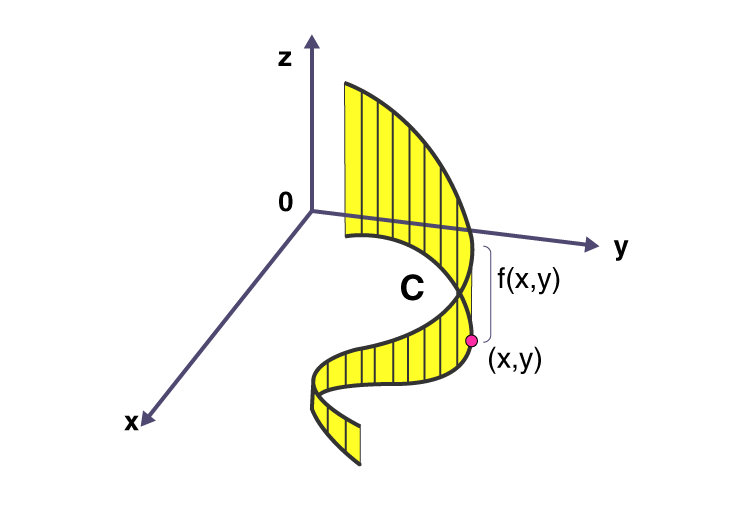
\includegraphics[width=0.5\textwidth]{Line-integral.png}
\end{center}

\textbf{Example: Scalar Field}

Compute the line integral of \(f(x,y) = x^2 + y^2\) over the straight line segment going
from \((1,1)\) to \((3,3)\)
\\
This time or curve is \(y = x\) to the parametrized curve is \(\begin{pmatrix}
    x(t) = t \\ y(t) = t
\end{pmatrix}\) this left us with:

\[
\int_{1}^{3}  2t^2 \sqrt{2}dt = \frac{52\sqrt{2}}{3} 
\]

\textbf{Example: Line Integral over a Vector Field}

Let \( f(x, y) = x^2 + y^2 \), and define a vector field based on its gradient:

\[
\vec{F}(x, y) = \nabla f(x, y) = \left( \frac{\partial f}{\partial x}, \frac{\partial f}{\partial y} \right) = (2x, 2y)
\]

Let the curve \( C \) be the quarter-circle of radius 1 from \( (1, 0) \) to \( (0, 1) \), parameterized by:

\[
\vec{r}(t) = (\cos t, \sin t), \quad t \in \left[0, \frac{\pi}{2}\right]
\]

We compute the line integral of \( \vec{F} \) along \( C \):

\[
\int_C \langle \vec{F}, d\vec{r}\rangle = \int_0^{\frac{\pi}{2}} \langle\vec{F}(\vec{r}(t)) \vec{r}'(t) \rangle\, dt
\]

First, compute:

\[
\vec{F}(\vec{r}(t)) = (2\cos t, 2\sin t), \quad \vec{r}'(t) = (-\sin t, \cos t)
\]

Now compute the dot product:

\[
\langle\vec{F}(\vec{r}(t)), \vec{r}'(t)\rangle = 2\cos t \cdot (-\sin t) + 2\sin t \cdot \cos t = -2\cos t \sin t + 2\cos t \sin t = 0
\]

Therefore, the line integral is:

\[
\int_C \langle \vec{F}, d\vec{r}\rangle = \int_0^{\frac{\pi}{2}} 0 \, dt = 0
\]

The line integral of the gradient vector field \( \vec{F} = \nabla f \) over this curve is zero. 
This is consistent with the fact that line integrals of gradient fields over 
curves depend only on endpoints, and 
\( f(1,0) = 1 \), \( f(0,1) = 1 \), so \( f(B) - f(A) = 0 \).


\subsection{Potential Function}

A vector field \( \vec{F} : \mathbb{R}^n \to \mathbb{R}^n \) is called \emph{conservative} if there exists a scalar function \( \phi : \mathbb{R}^n \to \mathbb{R} \) such that:

\[
\vec{F} = \nabla \phi
\]

The function \( \phi \) is then called a \emph{potential function} of \( \vec{F} \).

\textbf{Properties:}
\begin{itemize}[label=\(-\)]
    \item The line integral of \( \vec{F} \) over any path depends only on the endpoints:
    \[
    \int_\gamma \langle \vec{F}, d\vec{r} \rangle = \phi(B) - \phi(A)
    \]
    \item The line integral over a closed path is zero:
    \[
    \oint_\gamma \langle \vec{F}, d\vec{r} \rangle = 0
    \]
    \item \( \vec{F} \) is conservative \( \Leftrightarrow \) \( \vec{F} \) has zero curl in a simply connected region.
\end{itemize}

\subsection{Finding the Potential Function of a Vector Field}

To find the potential function \( \phi(x, y) \) of a vector field \( \vec{F}(x, y) = (P(x, y), Q(x, y)) \), we must check if the field is conservative and then integrate accordingly. A vector field is conservative if there exists a scalar potential function \( \phi \) such that:
\[
\vec{F} = \nabla \phi = \left( \frac{\partial \phi}{\partial x}, \frac{\partial \phi}{\partial y} \right)
\]

\textbf{Given:}
\[
\vec{F}(x, y) = \left(2xy + e^x,\ x^2 + \frac{1}{2\sqrt{y}}\right)
\]

Let \( P(x, y) = 2xy + e^x \), and \( Q(x, y) = x^2 + \frac{1}{2\sqrt{y}} \).

First, check if the field is conservative by verifying:
\[
\frac{\partial P}{\partial y} = \frac{\partial}{\partial y}(2xy + e^x) = 2x
\]
\[
\frac{\partial Q}{\partial x} = \frac{\partial}{\partial x}\left(x^2 + \frac{1}{2\sqrt{y}}\right) = 2x
\]

Since \( \frac{\partial P}{\partial y} = \frac{\partial Q}{\partial x} \), the field is conservative.

\textbf{Step 1: Integrate \( P(x, y) \) with respect to \( x \):}
\[
\phi(x, y) = \int (2xy + e^x)\,dx = x^2y + e^x + h(y)
\]
Here, \( h(y) \) is a function of \( y \) only.

\textbf{Step 2: Differentiate \( \phi(x, y) \) with respect to \( y \):}
\[
\frac{\partial \phi}{\partial y} = x^2 + h'(y)
\]

Set this equal to \( Q(x, y) = x^2 + \frac{1}{2\sqrt{y}} \), so:
\[
x^2 + h'(y) = x^2 + \frac{1}{2\sqrt{y}} \Rightarrow h'(y) = \frac{1}{2\sqrt{y}}
\]

\textbf{Step 3: Integrate to find \( h(y) \):}
\[
h(y) = \int \frac{1}{2\sqrt{y}}\,dy = \sqrt{y} + C
\]

\textbf{Final potential function:}
\[
\phi(x, y) = x^2y + e^x + \sqrt{y} + C
\]

Therefore, the potential function is:
\[
\boxed{\phi(x, y) = x^2y + e^x + \sqrt{y} + C}
\]


\subsection{Double Integral over a Rectangular Region}

Let \( A = [x_0, x_1] \times [y_0, y_1] \) be a rectangular region in \( \mathbb{R}^2 \). The double integral of a function \( f(x, y) \) over \( A \) is:

\[
\iint_A f(x, y)\, dA = \int_{x_0}^{x_1} \int_{y_0}^{y_1} f(x, y)\, dy\, dx
\]

\textbf{Note:} For rectangular domains, the order of integration does not affect the result:

\[
\int_{x_0}^{x_1} \int_{y_0}^{y_1} f(x, y)\, dy\, dx = \int_{y_0}^{y_1} \int_{x_0}^{x_1} f(x, y)\, dx\, dy
\]


\subsection{Integration over Curvilinear Domains}

If the region \( A \subset \mathbb{R}^2 \) is not rectangular, it is divided into subregions \( \Delta A_k \), and the integral is defined as the limit:

\[
\iint_A f(x, y)\, dA = \lim_{n \to \infty} \sum_{k=1}^n f(x_k, y_k) \, \Delta A_k
\]

In practice, for regions bounded by curves, we integrate in the form:
\[
\int_a^b \int_{u(x)}^{o(x)} f(x, y)\, dy\, dx
\]

Here, \( y \in [u(x), o(x)] \) describes the vertical bounds as functions of \( x \).

\textbf{Example}

Compute the volume under \(f(x,y) = 1 + x + y^2\) bounded by \(x\)-axis, \(x = 1\) and \(y\)-axis \(y = \sqrt{x}\)

\begin{center}
    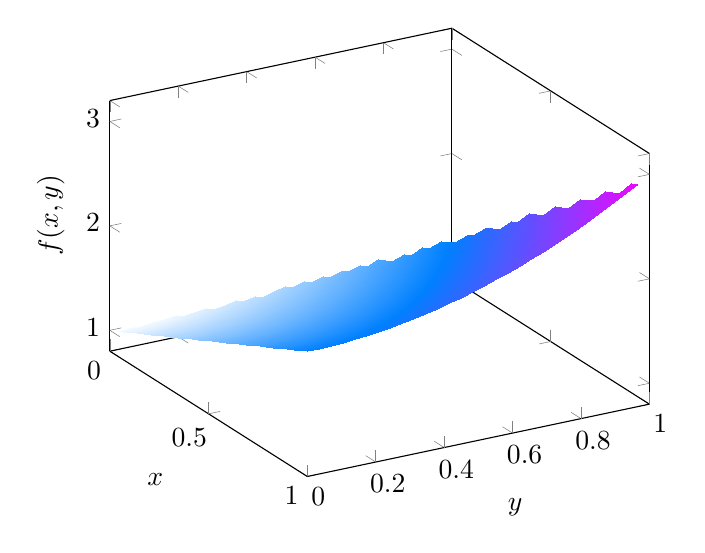
\begin{tikzpicture}
        \begin{axis}[
            view={60}{30},
            xlabel=$x$,
            ylabel=$y$,
            zlabel={$f(x,y)$},
            domain=0:1,
            y domain=0:1,
            samples=30,
            samples y=30,
            colormap/cool,
        ]
            \addplot3 [
                surf,
                domain=0:1,
                y domain=0:1,
                samples=30,
                samples y=30,
                restrict z to domain=-10:10,
                shader=interp,
            ]
            {y <= sqrt(x) ? 1 + x + y^2 : NaN};
        \end{axis}
    \end{tikzpicture}
\end{center}

First we are going to imagine slicing the area under this sector verticly along the \(x\)-axis from \(0\) up to \(1\) which
is the volume of an Area under a curve that is represented by going along the \(y\)-axis.

\begin{align*}
    \int_{0}^{1}\int_{0}^{\sqrt{x}} 1 + x + y^2 dydx \\
    \int_{0}^{1} \left| y + xy + \frac{y^3}{3} \right|_{0}^{\sqrt{x}} dx \\
    \int_{0}^{1} \left| \sqrt{x} + x\sqrt{x} + \frac{\sqrt{x}^3}{3} \right|_{0}^{\sqrt{x}} dx \\
    = \left| \frac{2}{3} x^{\frac{3}{2}} + \frac{4}{3} \frac{2}{5} x^{\frac{5}{2}} \right|_{0}^{1} = \frac{6}{5}
\end{align*}

If we choose the other way then we have an area with a fix \(y\) in the inside that goes from \(y^2\) to \(1\) with respect to \(x\).
\[
\int_{0}^{1}\int_{y^2}^{1} 1 + x + y^2 dxdy
\]

\subsection{Changing the order of integration to solve tricky integrals}

Given \(\int_{0}^{8}\int_{\sqrt[3]{x}}^{2} \frac{1}{y^4 +1}dydx\) which is very hard to integrate, lets change the order
to make it easier.

\[\int_{0}^{2}\int_{0}^{y^3} \frac{1}{y^4 +1}dxdy\]

The steps are the same as in the previous Example.

\begin{enumerate}
    \item Identify the area you want to integrate, what are the bounds respective to \(x\) and \(y\)
    \item Write the same expression without bounds and change the order of the differentials
    \item Imagine slicing the area underneath verticaly for \(x\) and horizontaly for \(y\) with their respective bounds corresponding
    to the perspective.
    \item Write the new integral with the opposite of order of integration
\end{enumerate}

\begin{center}

    Visualization of the area underneath the surface
    \smallskip

    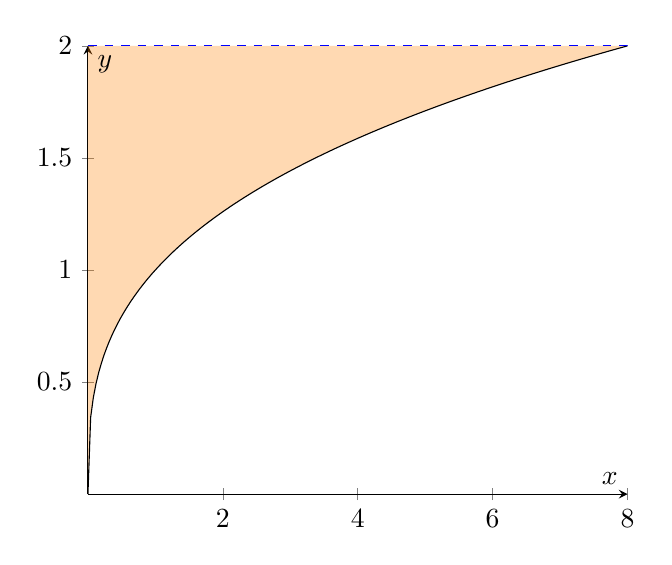
\begin{tikzpicture}
        \begin{axis}[
            axis lines=middle,
            xlabel={$x$},
            ylabel={$y$},
            legend pos=outer north east,
            domain=0:8,
            samples=200
        ]
            % Shading the area between the two functions
            \addplot [
                name path=A,
                domain=0:8,
                samples=200,
                draw=none
            ] {pow(x, 1/3)};
            
            \addplot [
                name path=B,
                domain=0:8,
                samples=200,
                draw=none
            ] {2};

            \addplot [
                orange,
                fill opacity=0.3
            ] fill between[of=A and B];

            % Plot both functions
            \addplot[color=black, domain=0:8, samples=200]{pow(x, 1/3)};

            \addplot[color=blue, dashed, domain=0:8, samples=200]{2};

        \end{axis}
    \end{tikzpicture}
\end{center}

Here the original bounds are: \(x\) goes from 0 to 8 and \(y\) goes from \(\sqrt[3]{x}\) to 2.
As you can see in the diagram by slicing vertically the value of \(x\) is fixed and we move towards the upper-bound of \(y\) which is 2.
Therefore the smallest \(x\) can get is 0 and the biggest is 2. While for \(y\) by slicing vertically we get that \(x\) goes from 0
to \(\sqrt[3]{x}\) but we do not want to left that y so we solve for y and get \(y^3\). Now we caput all of this together and integrate.


\subsection{The Jacobian}

The Jacobian matrix is a fundamental concept in multi-variable calculus. The Jacobian is best
approximation of a linear transformation for a point.

For the intuition of why, we use partial derivatives, just think about
how we use them as this tiny changes in the component of original
basis vectors.

Given a vector-valued function

\[
\mathbf{f} : \mathbb{R}^n \rightarrow \mathbb{R}^m, \quad f(x_1, \ldots, x_n) = 
\begin{bmatrix}
f_1(x_1, \ldots, x_n) \\
f_2(x_1, \ldots, x_n) \\
\vdots \\
f_m(x_1, \ldots, x_n)
\end{bmatrix},
\]
the \emph{Jacobian matrix} of \(f\) is the \(m \times n\) matrix of all first-order partial derivatives:
\[
J_f(x) = \begin{bmatrix}
\frac{\partial f_1}{\partial x_1} & \frac{\partial f_1}{\partial x_2} & \cdots & \frac{\partial f_1}{\partial x_n} \\
\frac{\partial f_2}{\partial x_1} & \frac{\partial f_2}{\partial x_2} & \cdots & \frac{\partial f_2}{\partial x_n} \\
\vdots & \vdots & \ddots & \vdots \\
\frac{\partial f_m}{\partial x_1} & \frac{\partial f_m}{\partial x_2} & \cdots & \frac{\partial f_m}{\partial x_n}
\end{bmatrix}.
\]

\subsubsection{Local linearity}
While performing non linear transformations on a space. We can see that in a tiny neighborhood
around a point, the transformation appears to be linear. And the matrix that encodes that
transformation is the \emph{Jacobian}.

For intuition, just imagine that in the tiny neighborhood the transformation is composed
of a small steps in the \(x_1, \dots, x_n\) directions which give of the partial derivatives that
represent this small steps. 

\subsubsection{Determinant}
When \(m = n\), i.e., the function maps from 
\(\mathbb{R}^n\) to \(\mathbb{R}^n\), 
the Jacobian matrix is square. In this case, 
the \textit{Jacobian determinant} is defined as:
\[
\det(J_{f}(x)),
\]
and provides important information about the local behavior of the function. For instance:
\begin{itemize}[label=\(-\)]
  \item If \(\det(J_{f}(x)) \neq 0\), the function is locally invertible at \(x\) by the inverse 
  function theorem.
  \item The sign and magnitude of the determinant 
  inform about orientation and volume scaling of the transformation.
\end{itemize}

When we change our systems of coordinates it is important
that our differential make sense in the original system we were.
Because of that, we take the determinant with respect to the new
coordinates to tell us the scaling factor that we have to use for our
result to make sense.

\textbf{Use Cases}
The Jacobian matrix and its determinant appear in many areas, including:
\begin{itemize}[label=\(-\)]
  \item \textbf{Change of variables in integrals:} The absolute value of the Jacobian determinant is used to adjust the measure when changing coordinates in multiple integrals.
  \item \textbf{Nonlinear optimization:} The Jacobian is crucial for computing gradients and performing techniques like Newton's method in multiple dimensions.
  \item \textbf{Differential equations:} Stability analysis of dynamical systems often involves evaluating the Jacobian at equilibrium points.
\end{itemize}

\subsubsection{List of Common Jacobians}

\begin{itemize}[label=\(-\)]

    \item \emph{Cartesian Coordinates}:
    \begin{itemize}
        \item Definition: The position of a point is given by \((x, y, z)\) in a 3D space along orthogonal axes.
        \item Jacobian: 
        \[
        J_{\text{Cartesian}} = 1dx
        \]
    \end{itemize}

    \item \emph{Polar Coordinates (2D)}:
    \begin{itemize}
        \item Definition: The position of a point in a plane is given by \((r, \theta)\), where \(r\) is the radial distance and \(\theta\) is the angle from the positive \(x\)-axis.
        \item Jacobian:
        \[
        J_{\text{Polar}} = rdrd\theta
        \]
    \end{itemize}

    \item \emph{Cylindrical Coordinates}:
    \begin{itemize}
        \item Definition: The position of a point in 3D space is given by \((r, \theta, z)\), where \((r, \theta)\) are the polar coordinates in the \(xy\)-plane and \(z\) is the height along the \(z\)-axis.
        \item Jacobian:
        \[
        J_{\text{Cylindrical}} = r\ dr d\theta dz
        \]
    \end{itemize}

    \item \emph{Spherical Coordinates}:
    \begin{itemize}
        \item Definition: The position of a point in 3D space is given by \((\rho, \theta, \phi)\), where:
        \begin{itemize}
            \item \(\rho\) is the distance from the origin,
            \item \(\theta\) is the azimuthal angle (in the \(xy\)-plane from the positive \(x\)-axis),
            \item \(\phi\) is the polar angle (from the positive \(z\)-axis).
        \end{itemize}
        \item Jacobian:
        \[
        J_{\text{Spherical}} = \rho^2 \sin (\phi) d\rho d\theta d\phi
        \]
    \end{itemize}

\end{itemize}

\subsection{Integration in Polar Coordinates}

For radially symmetric regions or functions, switching to polar coordinates simplifies the computation.

\textbf{Transformation:}
\[
x = r \cos \varphi, \quad y = r \sin \varphi
\]

The Jacobian of the transformation gives the area element:
\[
dA = r\, dr\, d\varphi
\]


\emph{Integral:}
\[
\iint_D f(x, y)\, dA = \int_{\varphi_0}^{\varphi_1} \int_{0}^{R(\varphi)} f(r \cos \varphi, r \sin \varphi)\, r\, dr\, d\varphi
\]

\subsubsection{Origin of the Area}
When we divide our circle in the sections we get both a difference in then angle and the radius which generate anorther area.
The difference \(\Delta A =\) Area of big wedge \(-\) Area of small wedge

\emph{Radius: }

\(r_k + \frac{\Delta r}{2}\) for the big wedge and \(r_k - \frac{\Delta r}{2}\) for the small wedge

\emph{Angle: }

\(\frac{\Delta \theta}{2 \pi}\) which is the angle of the fraction of the circle because the formula for the area is \(r^2 \pi\)
and the whole circle would be \(2\pi\)

\emph{Final Formula for the difference in the Area}

\[\Delta A = \frac{\Delta \theta}{2 \pi} \left ( \left[r_k + \frac{\Delta r}{2}\right]^2 - \left[r_k - \frac{\Delta r}{2}\right]^2\right)\] 
\[ = r_k \Delta r \Delta \theta\]

Which multiplied by the function value and by taking the limit of this sections we get that the volume:

\[
V = \int_{\theta_1}^{\theta_2} \int_{r_1 (\theta)}^{r_2 (\theta)} f(r, \theta) r \Delta r \Delta \theta
\]

\textbf{Example:}

\(f(r, \theta) = r\) above cardioid \(r = 1 - \sin \theta\)

Then

\[
V = \int_{0}^{2\pi}\int_{0}^{1 - \sin \theta} r r dr d\theta
\]

\[
= \int_{0}^{2\pi}\frac{r^3}{3} |_{0}^{1 - \sin \theta} d\theta = \int_{0}^{2\pi} \frac{(1 - \sin\theta)^3}{3} d\theta = \frac{5 \pi}{3}
\]


\subsection{Improper Integrals over Unbounded Regions}

If the domain of integration is unbounded (e.g., the entire plane \( \mathbb{R}^2 \)), the double integral is defined via a limit process:

\[
\iint_{\mathbb{R}^2} f(x, y)\, dx\, dy := \lim_{M_1, M_2 \to \infty} \lim_{N_1, N_2 \to \infty}
\int_{M_1}^{M_2} \int_{N_1}^{N_2} f(x, y)\, dy\, dx
\]

Often, using polar coordinates simplifies such cases, reducing multiple limits to one:

\[
\iint_{\mathbb{R}^2} f(x, y)\, dx\, dy = \int_0^{2\pi} \int_0^{\infty} f(r \cos \varphi, r \sin \varphi)\, r\, dr\, d\varphi
\]


\subsubsection{Gaussian Integral}

We are going to find the integral of the \emph{unbounded integral} 
\(e^{-x^2}\)using a combination of techniques.

\begin{align*}
S &= \int_{-\infty}^{\infty} e^{-x^2}dx\\
S^2 &= \left(\int_{-\infty}^{\infty} e^{-x^2}dx\right) \left(\int_{-\infty}^{\infty} e^{-x^2}dx\right)\\
S^2 &= \left(\int_{-\infty}^{\infty} e^{-x^2}dx\right) \left(\int_{-\infty}^{\infty} e^{-y^2}dy\right)
\end{align*}

Now lets translate to polar coordinates

\begin{align*}
S^2 &= \left(\int_{0}^{2\pi} \int_{0}^{\infty}re^{-(r\cos\theta)^2} re^{-(r\sin\theta)^2}drd\theta\right)\\
S^2 &= \left(\int_{0}^{2\pi} \int_{0}^{\infty}re^{-(r\cos\theta)^2 + (r\sin\theta)^2}drd\theta\right)\\
S^2 &= \left(\int_{0}^{2\pi} \int_{0}^{\infty}re^{-(r^2)}drd\theta\right)\\
S^2 &=  \left(\int_{0}^{2\pi} \int_{0}^{\infty}\frac{1}{2}e^{-(s)}dsd\theta\right)\\
S^2 &= \left(\int_{0}^{2\pi}d\theta\right)\\
S^2 &= \pi\\
S   &= \sqrt{\pi}
\end{align*}

\QED

\subsection{Triple Integrals}

The triple integral allows the computation of volume or mass in three-dimensional space.

Let \( V \subset \mathbb{R}^3 \) be a bounded region, then:

\[
\iiint_V f(x, y, z)\, dV = \lim_{n \to \infty} \sum_{k=1}^n f(x_k, y_k, z_k) \, \Delta V_k
\]

where \( \Delta V_k \) are small sub-volumes approximating \( V \).

In practice, evaluate:
\[
\iiint_V f(x, y, z)\, dz\, dy\, dx
\]

with limits determined by the geometry of the volume. The order of integration may be rearranged to simplify computation.

\[
\int_{x=a}^{x=b}\int_{y=g_1(x)}^{y=g_2(x)} \int_{f_1(x,y)}^{f_2(x,y)} dzdydx
\]

\subsubsection{Triple Integrals in Cartesian Coordinates}

In this short section we, will look at an example of how to calculate the volume enclose in
between two functions using triple integrals.

Given are the functions \(f_1(x,y) = x^2 + y^2\) and \(f_2(x,y) = 3 - x^2 - y^2\)

\newpage
\begin{center}
    
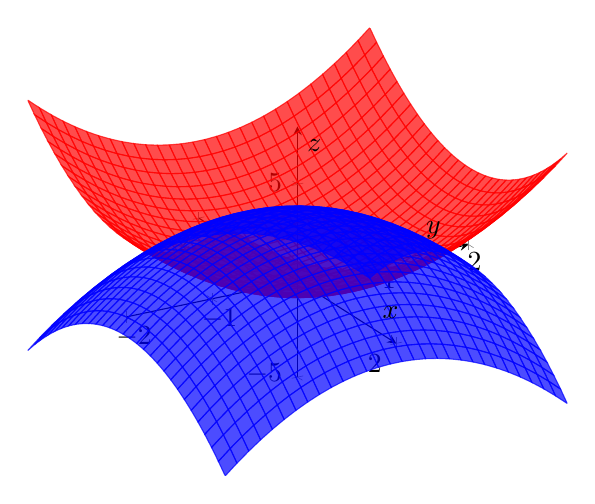
\begin{tikzpicture}
    \centering
    \begin{axis}[
        view={60}{30},
        axis lines=center,
        xlabel=$x$, ylabel=$y$, zlabel=$z$,
        domain=-2:2,
        y domain=-2:2,
        samples=30,
        samples y=30,
        colormap/jet,
    ]
        % Plot f1(x,y) = x^2 + y^2 in red
        \addplot3[
            surf,
            shader=flat,
            draw=red,
            fill=red,
            opacity=0.7,
        ]
        {x^2 + y^2};
    
        % Plot f2(x,y) = 3 - x^2 - y^2 in blue
        \addplot3[
            surf,
            shader=flat,
            draw=blue,
            fill=blue,
            opacity=0.7,
        ]
        {3 - x^2 - y^2};
    \end{axis}
\end{tikzpicture}
\end{center}

Lets find the intersection

\[
x^2 + y^2 = 3 -x^2 - y^2 
\]
\[
x^2 + y^2 = \frac{3}{2}
\]

Now we have to find the limits of integration for 
\[
\int_{x=a}^{x=b}\int_{y=g_1(x)}^{y=g_2(x)} \int_{f_1(x,y)}^{f_2(x,y)} dzdydx
\]

using our constraint and our original functions.

\[
\int_{x=a}^{x=b}\int_{y=-\sqrt{\frac{3}{2} - x^2}}^{\sqrt{\frac{3}{2} -x^2}} \int_{x^2 + y^3}^{3-x^2-y^2} dzdydx
\]

Here \(z\) means the height which is just the output
of the original functions.

The bounds of \(y\) just by looking at out constraint and solving for it.

And \(x\) only depends on the concrete limit of integration.


\subsubsection{Coordinate Transformation and the Jacobian Determinant}

Let a coordinate transformation be defined by:
\[
x = x(u, v, w), \quad y = y(u, v, w), \quad z = z(u, v, w)
\]

Then the triple integral transforms as:
\[
\iiint_{(x, y, z)} f(x, y, z)\, dx\, dy\, dz = \iiint_{(u, v, w)} f(x(u, v, w), y(u, v, w), z(u, v, w)) \cdot \left| \det J \right|\, du\, dv\, dw
\]

where \( J \) is the \emph{Jacobian matrix} of the transformation:
\[
J = 
\begin{pmatrix}
\frac{\partial x}{\partial u} & \frac{\partial x}{\partial v} & \frac{\partial x}{\partial w} \\
\frac{\partial y}{\partial u} & \frac{\partial y}{\partial v} & \frac{\partial y}{\partial w} \\
\frac{\partial z}{\partial u} & \frac{\partial z}{\partial v} & \frac{\partial z}{\partial w}
\end{pmatrix}
\]

\textbf{Example: Transformation to Cylindrical Coordinates}

The standard cylindrical coordinate transformation is:
\[
x = r \cos \varphi, \quad y = r \sin \varphi, \quad z = z
\]

The Jacobian determinant is:
\[
\left| \det J \right| =
\begin{vmatrix}
\cos \varphi & -r \sin \varphi & 0 \\
\sin \varphi & r \cos \varphi & 0 \\
0 & 0 & 1
\end{vmatrix}
= r
\]

Thus, the triple integral in cylindrical coordinates becomes:
\[
\iiint f(x, y, z)\, dx\, dy\, dz = \iiint f(r \cos \varphi, r \sin \varphi, z)\, r\, dr\, d\varphi\, dz
\]

\subsubsection{Calculating the center of mass with triple integrals}

We can make use of triple integration to calculate the center of mass of a body with
respect to \(x\), \(y\) or \(z\) with the following formulas:

\[x_s = \iiint_V xp(x,z,y)dz\ dy \ dx\]
\[y_s = \iiint_V yp(x,z,y)dz\ dy \ dx\]
\[z_s = \iiint_V zp(x,z,y)dz\ dy \ dx\]

Where \(p(x,y,z)\) is our mass function.

\newpage
\section{Differential Equations}

A Differential Equation is an equation that relates a function (the dependent variable)
with a variable or multiple variables (the independent variables) and its derivative.
\vspace{\baselineskip}

They can be categorized in \emph{Ordinary} and \emph{Partial} Differential Equations.

\subsection{Ordinary Differential Equations}

An equation of the form 

\[
    y^n = f(x, y, x', y', \dots, y^{n -1})
\]

is called \emph{Ordinary Explicit Differential Equations of order} \emph{n}
\vspace{\baselineskip}

If \(y^n = 0\) then it is \emph{implicit}
\vspace{\baselineskip}

If the exponent of the dependent variable is 1, and it
is build like a linear equation then it is categorized as \emph{Linear}

\subsection{Initial Value Problems and Solutions}

The specification of an explicit differential equation and the values

\[
    x_0,\quad y(x_0) = y_0,\quad y'(x_0) = y_1,\quad \dots,\quad y^{(n-1)}(x_0) = y_{n-1}
\]

is called an \emph{initial value problem (IVP)}.

An \emph{n}-times differentiable function \( y(x) \) that satisfies 
the explicit differential equation is called the \emph{general solution} of the 
differential equation. If it also satisfies the conditions of the initial value problem 
from the previous definition, it is called the \emph{particular solution} of the IVP\@.

\subsection{Volterra Integral}

The function \(y(x)\) is a solution of the IVP \(y' = f(x,y),\quad y(x_0) = y_0\) if and only if

\[
    y(x) = y_0 + \int_{x_0}^{x} f(t, y(t))dt
\]

\textbf{Proof:}

\[
    \int_{x_0}^{x} f(t, y(t))dt = \int_{x_0}^{x} y'
\]
\[
    y(x) = y(x_0)
\]

The other way would be

\[
    \left(\int_{x_0}^{x} f(t, y(t))dt + y_0\right)' = f(x, y(x)) = y' 
\]

\QED

\subsection{The Picard-Lindelöf Iteration Method}

We can approximate the desired solution using the Volterra integral equation as follows. 
Start with an arbitrary initial function, for example a constant — preferably the initial value:

\[
    g_0(x) = y_0
\]

Then form the next approximation to the desired function \( y(x) \) as:

\[
    g_{n+1}(x) = y_0 + \int_{x_0}^{x} f(t, g_n(t)) \, dt
\]

\subsection{Integration case}

To solve a ODE of the form \(y' = f(x)\) it is as easy as integrating \(f(x)\).

\subsection{Separation of Variables}

An equation \(F(x,y,y',\dots) = 0\) is a called an equation of \emph{separable variables} if it can
be written in one of the following forms:

\begin{itemize}
    
    \item \(\frac{dy}{dx} = f(x) g(y)\)
    
    \item \(\frac{dy}{dx} = \frac{f(x)}{g(y)}\)
    
    \item \(\frac{dy}{dx} = \frac{g(y)}{f(x)}\)

\end{itemize}

\subsubsection{Steps to solve a ODE of separable variables}

\begin{enumerate}

    \item Solve for the derivative

    \item Check that it is indeed an ODE of separable variables

    \item Separate the variables

    \item Integrate with respect to the independent variable

\end{enumerate}

\textbf{Example:}
\vspace{\baselineskip}

Given is \((y - 2)y' = 3x - 5\)

It is an ODE of separable variable

\[
    y' = \frac{3x - 5}{y - 2}
\]

Now we separate the variables and Integrate

\[
    \int (y - 2)y' dx = \int 3x - 5 dx
\]

Note that \(y' = \frac{dy}{dx}\) and \( \frac{dy}{dx} dx = dy\) (only as a convenient fiction
in reality we are changing the variables) thus,

\[
    \int (y - 2)dy = \int 3x - 5 dx
\]

\[
    \frac{y^2}{2} - 2y + c = \frac{3x^2}{2} - 5x + c
\]

The solution we get is an implicit solution. To make it look nice solve for \emph{y}
if you can.

\subsubsection{Understanding the fiction}

The previous fiction we used can explain in the following manner.
\vspace{\baselineskip}

Given \( f(y) \frac{dy}{dx} dx = \int f(y) dy\). We want to prove that this equality holds via the 
\emph{chain rule} \(\frac{du}{dx} = \frac{du}{dy} \frac{dy}{dx}\).

\begin{align*}
\frac{d}{dx} \left( \int f(y) dy \right) &= \frac{d}{dx} \left( \int f(y) dy \right) \frac{dy}{dx}\\
                                         &= f(y) dy \frac{dy}{dx}\\
                                         &\implies \int f(y) \frac{dy}{dx} = \int f(y) dy
\end{align*}
\QED

\subsection{Geometry of ODE}

You can imagine the plot of an ODE as a \emph{Slope field} where the slope (derivative) of a function
obeys a certain condition, this being the differential equation \(\frac{dy}{dx} = expr\).
\vspace{\baselineskip}

A point on this field is called an \emph{Initial Condition} and the curve that goes through
that point in the slope field is called an \emph{Integral curve} which a solution to the differential
equation with respect to that initial condition.

\subsection{Existence and Uniqueness}

Let \( f(x, y) \) be continuous on a rectangle \( [a, b] \times \Reals \). Then the differential 
equation

\[
    y' = f(x, y)
\]

has at least one solution. A unique solution is only guaranteed under additional conditions.

A function \( f : \Reals^2 \to \Reals \) is called 
\emph{Lipschitz continuous with respect to \emph{y}} if there exists a constant \( L > 0 \) such that

\[
    |f(x, y_1) - f(x, y_2)| \leq L |y_1 - y_2|
    \quad \text{for all } (x, y_1), (x, y_2) \in D.
\]

Let \( x_0 \in [a, b] \), and let \( f : [a, b] \times \Reals \to \Reals \) be continuous 
and bounded, and Lipschitz continuous in \emph{y}. Then the initial value problem

\[
    y' = f(x, y), \quad y(x_0) = y_0
\]

has a unique solution on \( [a, b] \).
\vspace{\baselineskip}

Or in easier words: If \emph{f} and \(\frac{\partial f}{\partial y}\) are continuous near \((x_0, y_0)\) 
then there is a unique solution on an interval \(\alpha < x_0 < \beta\) to the IVP

\[
    y' = f(x,y), \quad y(x_0) = y_0
\]

\subsection{How to deal with initial conditions}

After solving a differential equation we may have the problem that certain initial
conditions were set at the start, thus, making our general solution not specific.
\vspace{\baselineskip}

Solving this problem is pretty easy, because we just have to solve for the constant terms
in our general solution with respect to our initial conditions. Like for example \(y(0) = 1\)
we would plug 0 for all \emph{x}'s in our general solution the whole equation will be set equal to 1.

\subsection{Solving DE with Substitution}

In some cases a complex function can be simplified via a substitution.

\subsubsection{Case I}

\[
    y' = f(ax + by(x) + c)
\]

With a substitution like \(z(x) = ax + by(x) + c\) the right-hand side will become \(f(z)\)
and for the left-hand side we get \(y(x) = \frac{z(x) - ax - c}{b}\).
\vspace{\baselineskip}

Now we can substitute in the original equation, and we get

\[
    y'(x) = \frac{1}{b} (z'(x) - a) = f(z)
\]

\[
    z'(x) = a + b f(z)
\]

Now we can integrate and find the solution and then return to our original variables.
\vspace{\baselineskip}

\textbf{Example:}

\[
    y' = (x + y(x))^2
\]

Here \(a = 1\), \(b = 1\), \(c = 0\) and \(f(z) = z^2\)
\vspace{\baselineskip}

\textbf{1. Substitute}

\[
    z(x) = x + y(x)
\]
\[
    y(x) = z(x) - x
\]
\[
    y'(x) = z'(x) - 1
\]

\textbf{2. Plug in the DE}

\[
    y' = {(x + y(x))}^2
\]
\[
    z'(x) - 1 = {z(x)}^2
\]

\textbf{3. Integrate}

\[
    z'(x) = 1 + {z(x)}^2
\]
\[
    \frac{z'(x)}{1 + {z(x)}^2}
\]
\[
    \int \frac{1}{1 + z^2} dz = \int 1 dx
\]
\[
    \arctan (z) = x + c
\]
\[
    z = \tan(x + c)
\]

\textbf{4. Return to the original variables}

\[
    x + y(x) = \tan(x + c)
\]
\[
    y(x) = \tan(x + c) - x
\]

\subsubsection{Case II}

\[
    y' = f(\frac{y}{x})
\]

For this to be valid \(z(x) = \frac{y}{x}\) our \(y(x)\) needs to look like \(y(x) = z(x)x\) 
and so \(y' = z(x) + z'(x)x\).
\vspace{\baselineskip}

Now we substitute in the differential equation using \(f(z) = z(x) + z'(x)x\)

\[
    z'(x) = \frac{f(z) - z(x)}{x}
\]

Now we can integrate and then return to our original variables. \(y(x) = z(x)x \), where \(z(x)\) is our
result of the integration.
\vspace{\baselineskip}

\textbf{Example:}
\vspace{\baselineskip}

\[
    y' = \frac{y(x)}{x} + 1
\]

This in converted to \(y' = f(z) = z + 1\)
\vspace{\baselineskip}

\textbf{1. Substitute}

\[
    z(x) = \frac{y(x)}{x}
\]
\[
    y(x) = z(x)x
\]
\[
    y'(x) = z(x) + z'(x)x
\]

\textbf{2. Plug in the DE}

\[
    z(x) + z'(x)x = z(x) + 1
\]

\textbf{3. Integrate}

\[
    z'(x)x = 1
\]
\[
    \int z' dz = \int \frac{1}{x} dx
\]
\[
    z = (\ln(x) + c)x
\]

\subsection{Linear Differential Equations}

An ODE is called linear if all occurrences of the dependent variable and its
derivatives have an exponent of at most 1.

\[
    a_n(x)y^n + a_{n - 1}y^{n -1} + \cdots + a_1(x)y' + a_0(x)y = b(x)
\]

If such an Equation has also the property \(b(x) = 0\) it is called \emph{Homogeneous}

\subsubsection{How to solve a Linear Differential Equation}

In this case we will focus on first Order ODE\@.
\vspace{\baselineskip}

Write it in the standard form \(y' + p(x)y = f(x)\)
\vspace{\baselineskip}

Now use \emph{Integrating Factor Method}

\subsection{Integrating Factor Method}

We are going to multiply our expression by function \(r(x)\) 

\[
    r(x)y' + r(x)p(x)y = r(x)f(x)
\]

Now we would like to write the left side as \(\frac{d}{dx} y r(x)\) because now if we
were to integrate it would take us to the expression in the right.
\vspace{\baselineskip}

When we evaluate this new expression we get that

\[
    \frac{d}{dx} y r(x) = y'r(x) + r'(x)y
\]

which is not quite what we actually have, but it is close. Now note that we can say

\[
    r'(x) = r(x)p(x)
\]

This is a differential equation of separable variables thus, we can

\[
    \frac{r'(x)}{r(x)} = p(x)
\]

\[
    \int \frac{r'(x)}{r(x)}dx = \int p(x)dx
\]

\[
    \ln(r(x)) = \int p(x) dx
\]

after using \emph{e}

\[ 
    r(x) = e^{\int p(x) dx}
\]

Now we have found an \(r(x)\) and now that we know that such a function exists we can return 
to our initial problem and say

\[
    \frac{d}{dx}r(x)y = r(x)f(x)
\]

\[
    y = \frac{1}{r (x) } \int r (x) f (x) dx
\]

and 

\[
    r(x) = e^{\int p (x) dx}
\]

\textbf{Example:}
\vspace{\baselineskip}


Given are \(y' + 4y = e^{-x}\) and \(y(0) = \frac{4}{3}\)
\vspace{\baselineskip}

Here \(4 = p(x)\) and \(e^{-x} = f(x)\)
\vspace{\baselineskip}

Now let us use the formula for \(r(x) = e^{\int p (x)}\)
\vspace{\baselineskip}

this gives us \(r(x) = e^{\int 4dx} = e^{4x}\)
\vspace{\baselineskip}

Now recall what we saw earlier

\[
    e^{4x}y' + e^{4x}4y = e^{4x}e^{-x} = e^{3x}
\]

Our left side is just \(\frac{d}{dx} e^{4x}y\)
\vspace{\baselineskip}

Now let us complete the exercise with our last formula by integrating both sides

\[
    \frac{d}{dx} e^{4x}y = e^{3x}
\]
\[
    y = \frac{1}{e^4x}\int e^{3x}
\]
\[
    y = \frac{1}{e^4x} \frac{1}{3}e^{3x} + c
\]

Which is our general solution
\vspace{\baselineskip}

To find our specific solution we just plug 0 in to our general solution that gives us
\(\frac{1}{3} + c = \frac{4}{3}\) thus, \(c = 1\)

\subsection{Homogeneous Differential Equations}

A differential equation 

\[
    M(x,y)dx + N(x,y)dy = 0
\]

is considered \emph{Homogeneous} if and only if
\(M(x)\) and \(N(x)\) are \emph{homogeneous}, and they have the same degree.
\vspace{\baselineskip}

The equation \(y' + f(x)y = 0\) is called \emph{homogeneous linear differential equation of first order}.

\subsubsection{Homogeneous Equation}

A function \(f(x,y)\) is called \emph{homogeneous} if and only if it can be written

\[
    f(xt, yt) = t^n f(x,y)
\]

\textbf{Example: }

\[
    f(x,y) = x^3 + y^3
\]
\[
    f(tx, ty) = {(tx)}^3 + {(ty)}^3
\]
\[
    t^3 (x^3 + y^3) = t^3 f(x,y)
\]

It is important to note that the key is that each term have a total degree of \emph{n}.
For example: \(x^2y + x3y^2\)

\subsubsection{Homogeneous Functions Theorem}

If \(f(x,y)\) is homogeneous of degree \(0\) in \emph{x} and \emph{y} then 
\emph{f} is a function of \(\frac{y}{x}\)

Or \(f(x,y,y')\) is homogeneous if it can be written as \(y' = f(\frac{x}{y})\) or \(y' = f(\frac{y}{x})\)

\subsection{Solving Homogeneous DE I}

\begin{enumerate}
    \item Write in the form \(M(x,y)dx + N(x,y)dy = 0\)
    \item Check if it is homogeneous
    \item Change the variables to \(y = ux\) or \(x = uy\) depending on the situation
    \item Solve using the method of separable variables method
    \item Rewrite the answer in terms of the original variables again
\end{enumerate}

\textbf{Example:}
\vspace{\baselineskip}


Give is the function \((x -y)dx = - xdy\)
\vspace{\baselineskip}

\textbf{Step 1.} We write it in the desired form \((x - y)dx + xdy = 0\)
\vspace{\baselineskip}

\textbf{Step 2.} We notice that both are of degree \(1\). This time we skip the rigorous check.
\vspace{\baselineskip}

\textbf{Step 3.} We are going to choose the simpler function to do the change of variable 
depending on the \emph{differential!} 
\vspace{\baselineskip}

The simpler function is \(xdy\) thus, we are to change \emph{y}

\[
    y = ux
\]
\[
    dy = ux' + xu'
\]

and 

\[
    u = \frac{y}{x}
\]

Now substitute

\begin{align*}
    (x - ux)dx + x(udx + xdu) &= 0\\
    xdx - u x dx + x u dx + x^{2}du &= 0\\
    (x - ux + xu)dx + x^{2}du &= 0\\
    xdx + x^{2}du &= 0\\
    xdx &= - x^{2}du\\
    dx &= - xdu
\end{align*}

\textbf{Step 4.} Now we can integrate both sides

\[
    \int \frac{1}{x}dx = \int du
\]
\[
    \ln x + c = -u + c
\]

\textbf{Step 5.} No we use \(u = \frac{y}{x}\) to return to our original variables

\[
    \ln x + c = -\frac{y}{x} + c
\]
\[
    -x\ln x - xc = y
\]

\subsection{Solving Homogeneous DE I}

Another method for solving this kind of equations \(y' + f(x)y = 0\)is to follow the next steps.
\vspace{\baselineskip}

\textbf{Step 1: Separate the variables}

\[
    \frac{dy}{dx} = -f(x)y
\]

\textbf{Step 2: Use the separation of variables}

\[
    \int \frac{\frac{dy}{dx}}{y} = \int -f(x) dx
\]

\[
    \int \frac{dy}{y} = \int -f(x) dx
\]

\[
    \ln|y| = \int -f(x) dx
\]

\[
    y = C e^{\int -f(x) dx}
\]

This method works more directly.

\subsection{Inhomogeneous Equation}

The equation \(y' + f(x)y = g(x)\) is called \emph{linear inhomogeneous differential equation 
of first order} \(g(x)\) is called the \emph{distortion function}. The correspondent IVP is called
\emph{linear} IVP\@.

\subsection{Solutions of LDE}

Every linear IVP with continuous functions \(f(x)\) and \(g(x)\) plus a bounded \(f(x)\) 
has exactly one solution.
\vspace{\baselineskip}

\textbf{Proof:}

\begin{align*}
    y' = -f(x)y + g(x) \text{ therefore, } |-f(x)y_1 + g(x) + -f(x)y_2 + g(x) | &= |f(x)||y_1 - y_2|\\
                                                                            &\le M |y_1 - y_2|
\end{align*}

Therefore, the function is Lipschitz continuous, thus, a solution is possible.
\QED

\subsubsection{Variation of the Constants}

Recall that for the homogeneous case \(y' + f(x)y = 0\) case we use 
\(y = c e^{\int -f(x) dx}\), but now we have \(y' + f(x)y = g(x)\), thus, let us use the following
approach

\[
    y = c(x) e^{\int -f(x) dx}
\]

Now use the product rule to derivate

\begin{align*}
    y' &= c'(x) e^{\int -f(x) dx} + c(x)e^{\int -f(x) dx}(-f(x))\\
    &= c'(x)e^{\int -f(x) dx} - f(x)y
\end{align*}

thus, 

\[
    y' + f(x)y = c'(x)e^{\int -f(x) dx}
\]

therefore, \(g(x) = c'(x)e^{\int -f(x) dx}\)
\vspace{\baselineskip}

Then we can get a solution for \(c(x)\) from

\[
    g(x) = c'(x)e^{\int -f(x) dx}
\]
\[
    g(x) = c'(x)e^{-\int f(x) dx}
\]
\[
    c'(x) = \frac{g(x)}{e^{-\int f(x) dx}}
\]
\[
    c'(x) = g(x)e^{\int f(x) dx}
\]

\textbf{Example: }
\vspace{\baselineskip}

Given is \(y' -\cos(x)y = x e^{\sin(x)}\) with \(y(0) = 3\).
\vspace{\baselineskip}

\textbf{1. Solve as if it were homogeneous}

\begin{align*}
    y' -\cos(x)y &= 0\\
    y' &= \cos(x)y\\
    \frac{y'}{y} &= \cos(x)\\
    \int\frac{1}{y}dy &= \int \cos(x)dx \\
    \ln |y| + c &= \sin(x) + c \\
    y &= e^{\sin(x)}c 
\end{align*}

\textbf{2. Use \(y = c(x)e^{\sin(x)dx}\)}

\begin{align*}
    y' &= c(x)\cos(x)e^{\sin(x)} + c'(x)e^{\sin(x)}\\
    y' &= \cos(x)y + c'(x)e^{\sin(x)}\\
    y' - \cos(x)y &= c'(x)e^{\sin(x)}
\end{align*}
    
\textbf{3. Compare with the original equation}

\begin{align*}
    y' -\cos(x)y &= x e^{\sin(x)}\\
    y' - \cos(x)y &= c'(x)e^{\sin(x)}
\end{align*}

\textbf{4. Solve for \(c'(x)\)}

\begin{align*}
    xe^{\sin(x)} &= c'(x)e^{\sin(x)}\\
    x &= c'(x)
\end{align*}

\textbf{5. Integrate}

\begin{align*}
    \int x dx &= \int c'(x)dx\\
    \frac{x^2}{2} + c &= c(x)
\end{align*}

\textbf{6. Substitute in our approach \(y = g(x)e^{\sin(x)}\) from earlier}

\[
    y = \left(\frac{x^2}{2} + c\right)e^{\sin(x)}
\]

\textbf{7. Solve for \(c\) using our initial condition if asked}

\[
    y(0) = 3
\]
\[
    3 = \left(\frac{0^2}{2} + c\right)e^{\sin(0)}
\]
\[
    3 = c
\]

\subsection{Existence and Uniqueness Differential Equations}

For the IVP

\[
    y^{n} + p_{n - 1}y^{n - 1}+ \cdots + p_0 (x)y = f(x)
\]

\[
    y(a) = b_0, y'(a) = b_1, \dots, y^{n - 1}(a) = b_{n - 1}
\]

If all \(p_i\) and \emph{f} are continuous on the interval \emph{I} about \emph{a}, then
there exists a unique solution on \emph{I}.

\subsection{Constant Coefficients and the Superposition Theorem}

\subsubsection{Theorem of Superposition and the General Solution}

Suppose \(y_1, \dots, y_n\) solve 

\[
    y^{n} + p_{n - 1}y^{n - 1}+ \cdots + p_0 (x)y = 0
\]

Then \(y = c_1 y_1 + \cdots + c_n y_n\) also solves the equation, and it is the 
\emph{General Solution} if and only if the \emph{Wronskian} \(W(t) \ne 0\) for some \(t_0\).


\subsection{Undetermined Coefficients}

Given an equation \(y' + ay = g(x)\) notice that \emph{a} does not depend on \emph{x}.
The homogeneous equation to this case will be \(y' + ay = 0\) with a solution \(y_h\) and some
partial solution \(y_p\). Now remember from \emph{Linear Algebra} the 
\(general = particular + homogeneous\) more precisely \(y = y_p + y_h\) therefore, adding a 
particular solution to a homogeneous does not change
the general solution of our DE.
\vspace{\baselineskip}

Now let us substitute in our differential equation.

\begin{align*}
    (y_h + y_p)' + a(y_h + y_p) &= y_h' + y_p' + ay_h + ay_p\\   
    &= (y_h' + ay_h) + (y_p' + ay_p) = 0 + g(x) = g(x) 
\end{align*}

\subsubsection{Steps for solving Constant Coefficients problems}

\begin{enumerate}

    \item Find the \emph{homogeneous} solution for \(y' + ay = 0\). \(y_h\) is going
          to have a free parameter.
    
    \item Find a partial solution for \(y' + ay = g(x)\)
    
    \item Use \(y = y_h + y_p\)
    
    \item If you have an IVP solve for the free parameter in \(y_h\)

\end{enumerate}

Now we have to find a way to solve for \(y_p\) and \(y_h\)

\subsubsection{Find the partial solution}

We will use the method called based on guessing the type of the function on the right side.
\vspace{\baselineskip}

\textbf{Example: }
\vspace{\baselineskip}

Given is the following IVP: \(y' + 2y = 2x + 13\) with \(y(0) = 8\)
\vspace{\baselineskip}

By looking carefully we see that on the right-hand side we just have a normal polynomial,
thus, we can substitute \(y = bx + c\) and derivate \(y' = b\). In the case for when we have higher
order derivative we would differentiate for each of them. 
\vspace{\baselineskip}

Now substitute

\[
    b + 2(bx + c) = 2x + 13
\]

\[
    2bx + b + 2c = 2x + 13
\]

Now by comparing the Coefficients with the other side 

\[
    2b = 2
\]
\[
    b + 2c = 13
\]

We get: \(b = 1\), \(c = 6\). And we have found a \emph{particular} solution for our DE 
\(y_p = x + 6\)

Now we have to find a \emph{homogeneous} solution with the formula we already know
\(y_h = c e^{\int f(x)dx}\) in our case \(y_h = c e^{\int 2dx} = ce^{-2x}\)

\[
    y = y_h + y_p = c e^{-2x} + x + 6
\]

Now considering the condition \( y(0) = 8 \), this gives:

\[
    y(0) = c + 6 = 8 \Rightarrow c = 2
\]

and we obtain the particular solution:

\[
    y = 2 e^{-2x} + x + 6
\]

\subsubsection{Table of reference}
\bigskip
\begin{tabular}{|l|l|l|}
    \hline
    \textbf{Type of Forcing Function} & \textbf{Disturbance Function \( g(x) \)} & 
    \textbf{Approach for \( y_p \)} \\
    \hline
    Constant & \( k_0 \) & \( c_0 \) \\
    \hline
    Linear & \( k_0 + k_1 x \) & \( c_0 + c_1 x \) \\
    \hline
    Polynomial & \( \sum\limits_{i=0}^{n} k_i x^i \) & \( \sum\limits_{i=0}^{n} c_i x^i \) \\
    \hline
    Exponential & \( k e^{bx}, \; b \ne a \) & \( c_0 e^{bx} \) \\
               & \( k e^{ax} \) & \( c_0 x e^{ax} \) \\
    \hline
    Trigonometric & \( k \sin(bx) + l \cos(bx) \) & \( c_0 \sin(bx) + c_1 \cos(bx) \) \\
    \hline
\end{tabular}
\vspace{\baselineskip}

It is important to point out that sometimes it is necessary to combine different types
of functions to get the solution.
\vspace{\baselineskip}

\textbf{Example:}

\[
    y'' -2x' 3y = t^2  + 3e^{-t} \cos (4t)
\]

Here the approach would be

\[
    y_p = (A + Bt + Ct^2) + D(e^{-t}\cos(4t)) + E(e^{-t}\sin(4t))
\]

The best way is to tackle down each of the types of functions separately.
\vspace{\baselineskip}

An alternative to way of using this method is to

\begin{enumerate}

    \item Find the homogeneous solution.

    \item Multiply both sides of the equation by it.

    \item Integrate

\end{enumerate}

This will give you the exact same result and is faster.

\subsection{Bernoulli Equation}

This is used for equations of the form 

\[
    y' + P(x)y = Q(x)y^n
\]

We can not use the methods we already know for this equation because it is linear but with a
clever substitution we can turn it into a linear differential equation.
\vspace{\baselineskip}

Let us use a substitution 

\[
    u = y^{1 - n}
\] 

then 

\[
    u' = (1 - n)y^{-n} y'
\] 

Now this 
looks kinda similar to the original equation multiply by \(y^{-n}\) that looks like

\[
    y^{-n}y' + P(x)y^{-n}y = Q(x)y^{-n}y{n}
\]

\[
    y^{-n}y' + P(x)y^{1 - n} = Q(x)
\]


Notice that \(y^{-n} = \frac{u'}{(1-n)y'}\), thus, after substitution

\[
    \frac{1}{1 - n}u' + P(x)u = Q(x)
\]

Now our equation is \emph{linear}, and we can use the \emph{integrating factor} method.
\vspace{\baselineskip}

\textbf{Example: }
\vspace{\baselineskip}

Given is \(y' -5y = \frac{-5}{2}xy^3\).

\[
    u = y^{-2}  \text{ and } u' = -2y^{-3}y'
\]

\[
    y^{-3} = \frac{u'}{-2y'}
\]

And our equation after multiplying by \(y^{-3}\)

\[
    y^{-3}y' - 5yy^{-3} = -\frac{5}{2}x 
\]

\[
    y^{-3}y' - 5y^{-2} = -\frac{5}{2}x 
\]

\[
    \frac{u'}{-2y'}y' - 5u = -\frac{5}{2}x 
\]

Now we can use the \emph{Integrating Factor Method}. First bring to the standard form.
\(y' + p(x)y = f(x)\)

\[
  u' + 10u = 5x 
\]

Remember that \(r(x) = e^{\int p(x)dx} = e^{\int 10 dx} = e^{10x}\) therefore, we have

\[
    e^{10x}u' + 10ue^{10x} = e^{10x}5x
\]

Now let us integrate

\[
    \frac{d}{dx} \left(e^{10x}u\right) = e^{10x}5x
\]

\[
    Ce^{10x}u = \int e^{10x} 5x dx = 5x \frac{e^{10x}}{10} - \int e^{10x}5dx
\]

\[
    Ce^{10x}u = \int e^{10x} 5x dx = 5x \frac{e^{10x}}{10} - \frac{5}{10}\int e^{10x}dx
\]

\[
    Ce^{10x}u = \frac{xe^{10x}}{2} - \frac{5}{100} e^{10x} + c
\]

\[
    Ce^{10x} = \frac{x}{2} - \frac{1}{20} + \frac{c}{e^{10x}} = y^{-2}
\]

\subsection{Autonomous Equations}

An \emph{Autonomous Differential Equation} only depends on the dependent
variable \emph{y}.\textbf{ Example: } \(\frac{dy}{dt} = (1 + y)(1 -y)\).

\subsubsection{Equilibrium Solutions}

Values where \(f(y) = 0\) are \emph{Equilibrium Solutions}.

\subsubsection*{Asymptotically stable}

An equilibrium solution \(y = a\) is \emph{asymptotically stable} if solutions
that start near \emph{a} tend towards \emph{a} as \(t \to \infty\).

\subsubsection*{Asymptotically unstable}

An equilibrium solution \(y = a\) is \emph{asymptotically unstable} if solutions
that start near \emph{a} leave as \(t \to \infty\)

\subsection{Linear Inhomogeneous DEs with Non-Constant Coefficients}

The method of \emph{variation of constants} is often used alongside the \emph{superposition principle}. 
In this method, the integration constant in the function \( c(x) \) is omitted as it is part of the 
particular solution.
\vspace{\baselineskip}

The superposition principle also holds for linear inhomogeneous differential equations with 
non-constant coefficients:

\begin{align*}
    y_p' + f(x)y_p &= g(x) \quad \text{(particular solution)} \\
    y_h' + f(x)y_h &= 0 \quad \text{(homogeneous solution)}
\end{align*}

For the total solution \( y = y_h + y_p \), we get:

\begin{align*}
    y' + f(x)y 
    &= (y_h + y_p)' + f(x)(y_h + y_p) \\
    &= y_h' + y_p' + f(x)y_h + f(x)y_p \\
    &= g(x)
\end{align*}

Thus, the solution can be decomposed into the general solution of the homogeneous DE and a 
particular solution based on the form of the right-hand side.
\vspace{\baselineskip}

\textbf{Example: }

\[
    y' = -\frac{y}{x} + 1
\]

The homogeneous DE is \(y' = -\frac{y}{x}\) which can be solved by separating the variables.
\(y_h = \frac{c}{x}\)

Now let use \(y_p = \frac{c(x)}{x}\).

\[
    y_{p}' = \frac{c'(x)x - c(x)}{x^2}
\]

Let us break down the fraction to find where to put our homogeneous solution we have already found

\[
    \frac{c'(x)}{x} - \frac{c(x)}{x^2} = \frac{c'(x)}{x} + \frac{1}{x}\frac{c}{x} 
    = \frac{c'(x)}{x} + \frac{1}{x}y
\]

and we get

\[
    y_{p}' = -\frac{y}{x} + \frac{c'(x)}{x} 
\]

Here we compare with the inhomogeneous part of the original equation and get

\[
    \frac{c'(x)}{x} = 1 \implies c'(x) = x
\]

then \(c(x)\) is equal to \(\frac{x^2}{2}\) and therefore, \(y_p = \frac{x^2}{x}\frac{1}{x} = 
\frac{x}{2}\)
\vspace{\baselineskip}

As our final result we get \(y = \frac{c}{x} + \frac{x}{2}\)

\subsection{Power Series Approach}

Another method to solve a certain type  of differential equation
is to find the function given an initial conditions. This can be better understood with an example.

\[
    y' = y
\]
\[
    y(0) = 1
\]

We say \(y = \sum_{n = 0}^{\infty} a_n x^n\) and \(y(0) = a_0 = 1\).

Now let us derivate you \emph{y}

\[
    y = \sum_{n = 0}^{\infty} a_n x^n = a_0 x^0 + a_1 x^1 + \cdots = 1 + a_1 x^1 + a_2 x^2 + \cdots
\]
\[
    y' = 0  + a_1 + 2 a_2 x + 3 a_3 x^2 + \cdots 
\]

Thus, we can rewrite the sum as 

\[
    y' = \sum_{n = 1}^{\infty} a_n n x^{n - 1}
\]

Starting from 1 because 0 does not contribute to the sum. After shifting the index we get

\[
    y' = \sum_{n = 0}^{\infty} a_{n + 1}(n + 1)x^{n}
\]

Now we build our original DE with our new definitions for \(y'\) and \emph{y}

\[
    \sum_{n = 0}^{\infty} a_{n + 1}(n + 1)x^{n} = \sum_{n = 0}^{\infty} a_n x^n
\]

If we compare the coefficients we get

\[
    a_n = a_{n+1}(n+1)
\]

\[
    \frac{a_n}{(n + 1)} = a_{n+1}
\]


after iterating backwards we get

\[
    a_{n + 1} = \frac{a_n}{n + 1} = \frac{\frac{a_{n - 1}}{(n - 1 +1)}}{n + 1} = 
    \frac{\frac{\frac{a_{n - 2}}{(n - 1)}}{(n - 1 + 1)}}{n + 1}   
\]
\[
    a_n = \frac{a_0}{(n + 1)!} = \frac{1}{(n + 1)!} = 1
\]

therefore, \(a_n = \frac{1}{n!}\) which gives us the solution

\[
    \sum_{n = 0}^{\infty}\frac{1}{n!}x^n = e^x
\]

\subsubsection{Theorem for the Power Series of DE}

For a differential equation of the form:

\[
    A(x)y^{n} + \cdots + B(x)y' + C(x)y = 0
\]

more specific after dividing by \(A(X)\)

\[
    y^{n} + \cdots + P(x)y' + Q(x)y = 0,
\]

with \(x = a\) as an \emph{Ordinary Point} if \(\dots, P(x)\) and \(Q(x)\) are 
\emph{Analytic} at \(x = a\). Otherwise, a \emph{Singular Point}.
\vspace{\baselineskip}

Then this equation has \emph{n} linearly independent solutions of the form

\[
    y(x) = \sum_{n = 0}^{\infty} c_n {(x - a)}^n
\]

The radius of convergence is at least as large as distance to the nearest \emph{Singular Point}.

\subsection{Exact Differential Equations}

We will take a short look at functions with two inputs via implicit differentiation \(F(x,y(x)) = 0\).
We have:

\[
    F_x dx + F_y dy = 0
\]
\[
    p(x,y)dx + q(x,y)dy = 0
\]

after dividing by \(dx\)

\[
    F_x + F_y y' = 0
\]
\[
    p(x,y)dx + q(x,y)y' = 0
\]

If this is a differential then \(p_x = q_y\), and we define a DE of the form:

\[
    p(x,y)dx + q(x,y)y' = 0 \text{ with } p_x = q_y,
\]

as \emph{exact}. And the \(p_x = q_y\) as \emph{Integrability-Condition}.
\vspace{\baselineskip}

By finding the \emph{potential} we can solve this kind of differential equations.
\vspace{\baselineskip}

\textbf{Example:}
\vspace{\baselineskip}

\textbf{Step 1: Solve for \(y'\)}

\begin{align*}
    (12xy + 3)dx + 6x^2dy &= 0\\
    (12xy + 3) + 6x^2 y' &= 0\\
    y' = - \frac{12xy + 3}{6x^2}
\end{align*}

\textbf{Step 2: Test the Integrability-Condition}

\[
    p(x,y) = 12xy + 3
\]
\[
    q(x,y) = 6x^2
\] 
\[
    p_x = 12x
\]
\[
    q_y = 12x
\]

\begin{align*}
    F(x,y) &= \int (12xy + 3)dx = \int 6x^2 dy\\
        &= 6x^2 y + 3x + c(y) = 6yx^2 + c(x)
\end{align*}

Now we differentiate both sides with respect to \emph{y} and this gives us

\begin{align*}
    6x^2y + 3x + c(y) &= 6yx^2 + c(x) \\
    6x^2 + c'(y) &= 6x^2 \\
           c'(y) &= 0 \\
            c(y) &= y \text{ after integrating with respect to } dy,
\end{align*}

and therefore, \(F(x,y) = 6x^2y + 3x + \hat{c} = 0\).
\vspace{\baselineskip}

\textbf{Step 3: Solve for \emph{y}}

\[
    y = \frac{\hat{c} - 3x}{6x^2} 
\]

\subsubsection{Euler Multipliers}

Sometimes a seemingly \emph{exact} differential equations is not possible to solve do the partial 
derivatives of \(P(x,y)\) and \(Q(x,y)\) not being equal. An approach to this problem are the so-called 
\emph{Euler Multipliers}, which are some factor \(\mu(x) \text{ or } \mu(y)\) that when found. Can 
help solve the differential equation.

\[
    P(x,y)\mu(x) + Q(x,y)y'\mu(x) = 0
\]

or 

\[
    P(x,y)\mu(y) + Q(x,y)y'\mu(y) = 0
\]

The steps for solving this kind of problems are

\begin{enumerate}
    
    \item Choose either \(\mu(x)\) or \(\mu(y)\) and multiply the whole equation by it.
    
    \item Find the new partial derivatives of \(P\) and \emph{Q}.
    
    \item Set both partial equals and solve for \(\mu\) in the newly created differential equation 
          using the necessary method. Also make sure that the solution has no zeroes. This is necessary 
          because otherwise, we would have multiplied our original equation times zero.
    
    \item Substitute \(\mu\) with the solution. And if now both partials are equal then you can now 
          solve the exact differential equation. If not try with another \(mu\) using the other variable.
          And if this also does not work then the differential equation can not be solved. More specific, 
          if \(\mu(x)\) depends on \emph{y} and \(\mu(y)\) on \emph{x} then there is no way to make the 
          differential equation exact.

\end{enumerate}

\textbf{Example:}

\[
    3y^2 + 2xy y' = 0, x > 0 
\]

Here we have \(P(x,y) = 3y^2\) and \(Q(x,y) = 2xy\), whose partial derivatives are different

\[
    \frac{\partial P}{\partial y} = 6y \ne 2y = \frac{\partial Q}{\partial x}
\]

Now we try to use a multiplier \(\mu(x)\).

\[
    P_2 (x,y) = 3y^2 \mu(x) \text{ and } Q_2 (x,y)  = 2xy\mu(x)
\]

Now by taking the partials again

\begin{align*}
    \frac{\partial P_2}{\partial y} &= 6y\mu(x)\\  
    \frac{\partial Q_2}{\partial x} &= 2y(\mu(x) + x\mu'(x))  
\end{align*}

Now by setting them equal \(6y\mu(x) = 2y(\mu(x) + x\mu'(x))\) we can solve a new differential equation 
to find \(\mu(x)\) and \(\mu'(x)\).  

\begin{align*}
    6y\mu(x) &= 2y(\mu(x) + x\mu'(x)) \\
    3\mu(x) &= \mu(x) + x\mu'(x) \\
    2\mu(x) &= x\mu'(x)\\
    2\mu &= x \frac{d\mu}{dx} \\
    \int \frac{2}{x}dx &= \int \frac{d\mu}{\mu} \\
    2\ln(x) &= \ln(\mu) \\
    \mu &= x^2
\end{align*}

Now finally we check if now the partials are equal, which in this case is true.

\begin{align*}
    \frac{\partial P_2}{\partial y} &= 6yx^2\\  
    \frac{\partial Q_2}{\partial x} &= 6yx^2  
\end{align*}

Now the equation can be solved like normal.

\subsection{Constant Coefficients ODE}

Consider the second-order linear differential equation with constant coefficients:

\[
    a y'' + b y' + c y = 0,
\]

where \( a, b, c \in \Reals \), and \( a \neq 0 \).

We look for solutions of the form \( y = e^{rt} \). Substituting into the equation:

\begin{align*}
    y &= e^{rt}, \\
    y' &= r e^{rt} \\
    y'' &=  r^2 e^{rt}
\end{align*}


Substituting into the original equation:

\[
    ar^2 e^{rt} + bre^{rt} + ce^{rt} = 0
\]

Factoring out \( e^{rt} \) (which is never zero):

\[
    e^{rt}(ar^2 + br + c) = 0 \quad \Rightarrow \quad ar^2 + br + c = 0.
\]

This is a quadratic equation in \( r \). Solving using the quadratic formula:

\[
    r = \frac{-b \pm \sqrt{b^2 - 4ac}}{2a}.
\]

Suppose there are two linearly independent solution \(y_1\) and \(y_2\) to

\[
    y'' + p(x)y' + q(x)y = 0,
\]

then the general solution is \(y = c_1 y_1 + c_2 y_2\).
\vspace{\baselineskip}

We analyze the nature of the roots \( r \) based on the discriminant \( D = b^2 - 4ac \).
Also, for dealing with initial conditions of the form \(y^n = a, \dots\) we only have to 
plug the values into our solutions \(y_h, y_{h}', \dots \) to get the constants.

\subsubsection{Case 1: Two Distinct Real Roots \texorpdfstring{\( (D > 0) \)}{}}

There not much not to just plug the solutions of the root.

\[
    y = c_1 e^{r_1 t} + c_2 e^{r_2 t}
\]

\subsubsection{Case 2: Repeated Real Root \texorpdfstring{\( (D = 0) \)}{}}

For this case we need to use a trick.

\[
    y = c_1 e^{rt} + c_2 te^{rt}
\]

Note that this could be contra intuitive but \(te^{rt}\) is a solution and is linearly independent.
For more repeated roots you can use higher powers of \emph{t} \(t, t^2, t^3, \dots\).

\subsubsection{Case 3: Complex Conjugate Roots \texorpdfstring{\( (D < 0) \)}{}}

When the discriminant \( D = b^2 - 4ac < 0 \), the roots of the characteristic equation are complex:

\[
    r = \alpha \pm i\beta,
\]

where \( \alpha = -\frac{b}{2a} \) and \( \beta = \frac{\sqrt{4ac - b^2}}{2a} \).

The general solution to the differential equation is:

\[
    y(t) = c_1 e^{(\alpha + i\beta)t} + c_2 e^{(\alpha - i\beta)t}.
\]

To express this in real form, we use Euler’s formula:

\[
    e^{i\beta t} = \cos(\beta t) + i\sin(\beta t).
\]

Now rewrite each exponential term:

\begin{align*}
    e^{(\alpha + i\beta)t} &= e^{\alpha t} \cdot e^{i\beta t} = e^{\alpha t} (\cos(\beta t) + i \sin(\beta t)), \\
    e^{(\alpha - i\beta)t} &= e^{\alpha t} \cdot e^{-i\beta t} = e^{\alpha t} (\cos(\beta t) - i \sin(\beta t)).
\end{align*}

Now to get rid of the imaginary part we can do the following trick

\[
    \frac{y_1 + y_2}{2} = e^{\alpha t}\cos\beta t
\]
\[
    \frac{y_1 - y_2}{2i} = e^{\alpha t}\sin\beta t
\]

This might feel wrong, but these are in fact linear combinations of our original solution,
and they are also linearly independent, because of that we can just use them for our general solution.

\[y = c_1 e^{\alpha t}\cos\beta t + c_2  e^{\alpha t}\sin\beta t\]

\textbf{Example:}
\vspace{\baselineskip}

Given is \(y''\,' + y' = 0\).

\[
    y = e^{rt}
\]

\begin{align*}
r^3 + r &= 0\\
r(r^2 + 1) &= 0\\
r(r + i)(r - i) &= 0
\end{align*}

Now \(r_1 = 0 \quad r_2 = -i \quad r_3 = i\)

\[
    y = c_1 e^{0t} + c_2 e^{-it} + c_3 e^{it}
\]

\[
    y = c_1 + c_2 \cos t + c_3 \sin t
\]

\subsubsection{Inhomogeneous Case}

For the inhomogeneous case we would apply the method of the \emph{Undetermined Coefficients}. But 
differentiating two times or more depending on the order of the differential equation.

\subsection{The Wronskian}

Let \( y_1, y_2, \ldots, y_n \) be \emph{n} functions that are at least 
\( (n-1) \)-times differentiable on some interval. The \emph{Wronskian} of these 
functions is defined as:

\[
    W(y_1, y_2, \ldots, y_n)(x) =
    \begin{vmatrix}
    y_1(x) & y_2(x) & \cdots & y_n(x) \\
    y_1'(x) & y_2'(x) & \cdots & y_n'(x) \\
    \vdots & \vdots & \ddots & \vdots \\
    y_1^{(n-1)}(x) & y_2^{(n-1)}(x) & \cdots & y_n^{(n-1)}(x)
    \end{vmatrix}
\]

If \(W(A) \ne 0\) then they are linearly independent.


\subsection{Linearity Property}

Let \( y_p^{(1)} \) be a particular solution of  

\[
    y'' + ay' + by = g_1(x)
\]  

and \( y_p^{(2)} \) a particular solution of  

\[
    y'' + ay' + by = g_2(x),
\]  

then  

\[
    y_p = y_p^{(1)} + y_p^{(2)}
\]  

is a particular solution of  

\[
    y'' + ay' + by = g_1(x) + g_2(x).
\]  

\subsection{Variation of Parameters}

For a linear differential equation of the form

\[
    y'' + p(x)y' + q(x)y = f(x)
\]

The homogeneous equation has a solution of the linearly independent \(y_1\) and \(y_2\)
of the form \(y = u_1 y_1 + u_2 y_2\). We can guess the functions \(y_1\) and \(y_2\).
\vspace{\baselineskip}

So, for finding a solution of these types of equations we use the following formulas.

\[
    u_1 = - \int \frac{y_2 g}{y_1 y_{2}' - y_2 y_{1}'} dx
\]


\[
    u_2 = - \int \frac{y_1 g}{y_1 y_{2}' - y_2 y_{1}'} dx
\]

These formulas come from:
\vspace{\baselineskip}

\textbf{Differentiating two times:}

\[
    y = u_1 y_1 + u_2 y_2
\]

\[
    y' = u_1 y_{1}' + y_1 u_{1}' +  u_2 y_{2}' + y{2} u_{2}'
\]

Here we can add another constraint that \(y_1 u_{1}' + y{2} u_{2}' = 0\). This allows us to
simplify the expression to:

\[
    y' = u_1 y_{1}' +  u_2 y_{2}'
\]

Now we can derivate one more time:

\[
    y'' =  u_1 y_{1}'' + y_{1}' u_{1}'  + u_2 y_{2}'' + y_{2}' u_{2}'
\]


\textbf{Substitute in the original equation}

\[
    y'' + p(x)y' + q(x)y = f(x)
\]

\[
    u_1 y_{1}'' + y_{1}' u_{1}'  + u_2 y_{2}'' + y_{2}' u_{2}' + p(x)(u_1 y_{1}' +  u_2 y_{2}') 
    + q(x)(u_1 y_1 + u_2 y_2) = g(x)  
\]

\[
    u_1 y_{1}'' + y_{1}' u_{1}'  + u_2 y_{2}'' + y_{2}' u_{2}' + p(x)(u_1 y_{1}') + p(x)(u_2 y_{2}') 
    + q(x)(u_1 y_1) + q(x)(u_2 y_2) = g(x)  
\]

\[
    u_1 y_{1}'' + y_{1}' u_{1}'  + u_2 y_{2}'' + y_{2}' u_{2}' + p(x)(u_1 y_{1}') + p(x)(u_2 y_{2}') 
    + q(x)(u_1 y_1) + q(x)(u_2 y_2) = g(x)  
\]

With non-generic function a lot of the terms would cancel out. After that we add multiply by
\(y_1\) one of the rows and \(y_2\) so that we can cancel them in a row operation. Which will left us
with only two integrals to solve.

\subsection{Which method to use depending on the type of differential equations}

\subsubsection{First Order}

\begin{itemize}

    \item Separable \(\Rightarrow\) Separation of Variables.

    \item Form \(y' = f(ax + by(x) + c)\) \(Rightarrow\) Substitution \(z = ax + by(x) + c\) and \(f(z)\).

    \item Form \(y' = \frac{y}{x}\) \(\Rightarrow\) Substitution \(z = \frac{y}{x}\)

    \item Linear \(\Rightarrow\) Integrating Factor or Variation of Constants.

    \item Bernoulli (Non-linear) \(\Rightarrow\) Bernoulli Substitution.

    \item Autonomous \(\Rightarrow\) Equilibrium Analysis.

    \item Non-homogeneous \(\Rightarrow\) Undetermined Coefficients or integrating factor.

\end{itemize}


\subsubsection{Second Order and higher}

\begin{itemize}

    \item Constant Coefficients \(\Rightarrow\) Guess \(e^{rx}\).

    \item Non-homogeneous \(\Rightarrow\) Undetermined Coefficients.

    \item Linear \(\Rightarrow\) Series Solutions.

\end{itemize}

\subsubsection{Exact}

Using the method for exact differential equations.

\subsection{Linear Systems of Differential Equations}

Let us start by looking at a system of first order homogeneous differential equations

\[
    y_1 ' = ay_1 + by_2
\]
\[
    y_2 ' = cy_1 + dy_2
\]

This can be written as 

\[
    \frac{d}{dt} 
    \begin{pmatrix} 
    y_1 \\ 
    y_2 
    \end{pmatrix} 
    = 
    \begin{pmatrix}
    a & b \\
    c & d \\
    \end{pmatrix} 
    \begin{pmatrix}
    y_1 \\ 
    y_2
    \end{pmatrix}
\]

\[
    Ax = \vec{y}'
\]

Then if we use the guess \(y(t) = \vec{v} e^{\lambda t}\) and differentiate with respect to \emph{t} 
we get 

\[
    \lambda \vec{v} e^{\lambda t} = A \vec{v} e^{\lambda t}
\]

\[
    \lambda \vec{v} = A \vec{v},
\]

which is our \emph{Eigenvalue} problem. This can be solved via

\[
    \det(A - \lambda I) = 0
\]

\[
    \lambda^{2} - (a + c)\lambda + ad - bc = 0
\]

And this solution can lead to the three cases we already know: distinct real roots, complex Conjugate 
roots and repeated roots.
\vspace{\baselineskip}

We can also use substitution to solve for one of the \(y_i\), which are functions of \emph{x} like

\begin{align*}
    y_1 ' &= ay_1 + by_2\\
    y_2 ' &= cy_1 + dy_2\\
    by_2 &= y_1' - ay_1\\
    y_2 & \frac{y_1' - ay_1}{b}
\end{align*}


Then we can differentiate our first equation with respect to \emph{x}


\begin{align*}
    by_2 &= y_1' - ay_1\\
    by_2' &= y_1'' - ay_1'\\
    &= b (cy_2 + dy_1)\\
    &= bcy_2 + bdy_1\\
    &= c (y_1' -ay_1 ) + bdy_1\\
    y_1'' - (a + c)y_1' + (ac - bd)y_1 + bdy_1 &= 0
\end{align*}



\textbf{Example:}
\vspace{\baselineskip}

We are given the system of differential equations:

\[
    \begin{cases}
    y' = y + z \\
    z' = -2y + 3z
    \end{cases}
\]

We write this system in matrix form:

\[
    u' = Au, \quad \text{where } u = \begin{bmatrix} y \\ z \end{bmatrix}, \quad A = \begin{bmatrix} 1 & 
        1 \\ -2 & 3 \end{bmatrix}
\]

To solve, we find the eigenvalues of \emph{A} by solving the characteristic equation:

\[
    \det(A - \lambda I) = 
    \begin{vmatrix}
    1 - \lambda & 1 \\
    -2 & 3 - \lambda
    \end{vmatrix}
    = (1 - \lambda)(3 - \lambda) + 2 = \lambda^2 - 4\lambda + 5 = 0
\]

Solving the quadratic equation:

\[
    \lambda = \frac{4 \pm \sqrt{(-4)^2 - 4(1)(5)}}{2} = \frac{4 \pm \sqrt{-4}}{2} = \frac{4 \pm 2i}{2} 
    = 2 \pm i
\]

Now we find an eigenvector corresponding to \( \lambda = 2 + i \) by solving:

\[
(A - (2 + i)I)v = 0
\]

\[
    A - (2 + i)I = \begin{bmatrix} 1 - (2 + i) & 1 \\ -2 & 3 - (2 + i) \end{bmatrix}
    = \begin{bmatrix} -1 - i & 1 \\ -2 & 1 - i \end{bmatrix}
\]

From the first row of the system:

\[
    (-1 - i)v_1 + v_2 = 0 \Rightarrow v_2 = (1 + i)v_1
\]

So, an eigenvector corresponding to \( \lambda = 2 + i \) is:

\[
    v = \begin{bmatrix} 1 \\ 1 + i \end{bmatrix}
\]

After repeating the previous computation for \(\lambda = 2 - i\) we get the complex solution to the 
system:

\[
    u(t) = c_1 e^{(2 + i)t} \begin{bmatrix} 1 \\ 1 + i \end{bmatrix}
    + c_2 e^{(2 - i)t} \begin{bmatrix} 1 \\ 1 - i \end{bmatrix}
\]















\section{Probability}

\subsection{Basics}

\subsubsection{Probability}

\(E\) is the choosen event and \(\Omega\) the total. Example \(\frac{1}{2}\)

\[P(E) = \frac{E}{\Omega}\]

\subsubsection{Expected Result}

Here \(p\) represenst the probability of 
something and \(x\) the expected reward

\[E(x) = p_1 x_1 + \cdots + p_n x_n\]

\subsection{Standard Deviation}

\[
\sigma = \sqrt{ \frac{ (\overline{x} - x_1)^2 + \cdots + (\overline{x} - x_n)^2 }{ n } }
\]


\subsection{Binomial Distribution}

\textbf{Formulas:}

\begin{itemize}[label=\(-\)]
    \item \emph{Probability: } \(P(X = k) = \binom{n}{k} p^k (1 - p)^{n - k}\)
    \item \emph{Expected Result: } \(E(X) = n * p\)
    \item \emph{Standard Deviation: } \(\sqrt{E(X)(1-p)}\)
    \item  \emph{Varianz: } \(E(x)(1-p)\)
\end{itemize}

\subsubsection{Continuous Probability}

\[
\sum_{i = P(X=k)}^{P(X=n) (P(X=i))}
\]

\textbf{Formulas: }

\begin{itemize}
    \item \(P(X = a) = P(X = a)\)
    \item \(P(X \le a) = P(X \le a)\)
    \item \(P(X < a) = P(X \le a - 1)\)
    \item \(P(X > a) = 1 - P(X \le a)\)
    \item \(P(X \ge a) = 1 - P(X \le - 1)\)
    \item \(P(a \le X \le b) = P(X \le b) - P(X \le a)\)
\end{itemize}

\subsubsection{Sigma Rules}

\begin{itemize}[label = \(-\)]
    \item \(P(\mu - \sigma \le x \mu + \sigma) \approx 68,3\%\)
    \item \(P(\mu - 2\sigma \le x \mu + 2\sigma) \approx 95,4\%\)
    \item \(P(\mu - 3\sigma \le x \mu + 3\sigma) \approx 99,7\%\)
\end{itemize}

\subsection{Normal Distribution}

\begin{itemize}[label=\(-\)]
    \item \emph{Probability: } \(\frac{1}{\sqrt{2\pi \sigma^2} e^{\frac{1}{2} \left(\frac{x - u}{\sigma}\right)^2}}\)
    \item \emph{Expected Result: } \(E(x) = np = \mu\)
    \item \emph{Varianz: } \(Var(x) = E(X) (1-p)\)
    \item \emph{Standard Deviation: } \(\sqrt{Var(x)}\)
\end{itemize}

\subsection{Conditional Probability}

Probability of \(a\) under the condition \(b\).

\[P_b (a) = \frac{P(b \cap a)}{P(b)}\]

\subsubsection{Formula for the Total Probability}

\[P(a) = P_b (a) P(b) + P_{\neg b}(a) P(\neg b)\]

\subsection{Bayes Theorem}

\[P(a | b) = \frac{P(b | a) P(a)}{P(b)}\]

\subsection{Hypergeometric Distribution}

\[P(X = k) = \frac{\binom{M}{K} \binom{N - M}{n - K}}{\binom{N}{n}}\]

\textbf{Nomenclature}
\begin{itemize}[label=\(-\)]
    \item \(N\): Total number of elements
    \item \(M\): Elements with the trait \(A\)
    \item \(N - M\): Elements withou the trait \(A\)
    \item \(n = k\): Number to elements to take
\end{itemize}

\textbf{Formulas }
\begin{itemize}[label=\(-\)]
    \item \emph{Expected Results: } \(E(x) = n \frac{M}{N}\)
    \item \emph{Varianz: } \(Var(X) = E(x)\left(1 - \frac{M}{N}\right) \left(\frac{N - n}{N - 1}\right)\)
\end{itemize}

\newpage

\newpage
\section{Combinatorics}

\subsection{Permutation}

Number of ways of ordering \(n\) distinct elements.

\[n!\]

\subsection{Permutation with repetition}

Number of ways of ordering \(n\) non distinct elements. Here \(m_1, \dots, m_n\)
is the number a specific item is repeated in the original set.

\[\frac{n!}{m_1! \cdots m_n!}\]

\subsection{Variation}

Ways of put \(n\) objects in \(k\) slots with repetition.

\[n^k\]

\subsection{Variation without repetition}

Ways of put \(n\) objects in \(k\) slots without repetition.

\[\frac{n!}{(n -k)!}\]

\subsection{Combination I}

Ways of choose \(k\) objects of \(n\) elements.

\[\binom{n}{k} = \frac{n!}{k!(n-k)!}\]

Here \(n!\) is the number of permutations of the original set.
\((n-k)!\) has the function of eliminating the permutations of elements we are not interested in, and
\(k!\) is to eliminate the duplicates because for a combination the order does not matter, contrary to
the permutations.

\subsection{Combination II}

This focuses not on the slots but in the separations between the slots.
More specific the number of ways to distribute \(k\) identical objects into \(n\) identical boxes. 

\[\binom{n + k - 1}{k} = \frac{(n + k - 1)!}{k!(n - 1)!}\]

\subsection{Disarray}

Number of permutation in which no object ends in the same initial spot. Also know as the \textbf{subfactorial}

\[!n = n! \sum_{k = 0}^{n} \left(\frac{{(-1)}^k}{k!}\right)\]

\subsection{Bell Numbers}

Number of ways of grouping \(n\) objects in an arbitrary number of slots.

\[B(N) = \sum_{k = 0}^{N-1}\binom{N}{K}B(K)\]

with \(B(1) = 1\) and \(B(2) = 2\)

\subsection{Ramanujan Numbers}

The same as the Bell Numbers but, all objects are equal. As an example the number of ways
to decompose a number.

\[R(N) \approx \frac{1}{4N\sqrt{3}} e^{2\pi \sqrt{\frac{N}{6}}}\]

\subsection{Stirling Numbers I}

Ways of permuting \(N\) items with \(K\) exchanges.

\[ \left[ N + 1 \atop K\right] = N\left[N \atop K\right] + \left[N \atop K - 1\right]\] 

\subsection{Stirling Numbers II}

Ways of grouping \(n\) items in \(k\) slots.

\[ \left\{ \begin{matrix} N \atop K \end{matrix}\right\} = \frac{1}{K!} \sum_{j=0}^{K}{(-1)}^{k - j}\binom{K}{j}j^N \]

\subsection{Lah Numbers}

Ways of building \(K\) lists with a set \(N\) elements.

\[\left\lfloor \begin{matrix} N \atop K \end{matrix}\right\rfloor  = \binom{N - 1}{K - 1}\frac{N!}{K!} = \sum_{j=0}^{K}\left[N \atop K\right]\left\{N \atop K\right\}\]

\subsection{Euler's Numbers}

Number of permutations of a set of \(N\) elements of different size in which
\(K\) elements are bigger than the their previous element.

\[\left\langle \begin{matrix} N \atop K \end{matrix}\right\rangle = \sum_{j = 0}^{k}{(-1)}^j \binom{N + 1}{j}{(K +1 -j)}^N\]

\subsection{Catalan Numbers}

This ones have different applications like the number of ways of the triangulations of
a polygon or the number of trees with \(N\) leafs.

\[\mathfrak{C}(N) = \binom{2N}{N} - \binom{2N}{N + 1}\]

or

\[\mathfrak{C}(N) = \sum_{k=1}^{n}(k - 1) \mathfrak{C}(N - k)\]

\subsection{Pascals Triangle}

This is a triangle build by the formula \(\binom{n + 1}{k + 1} = \binom{n}{k}\binom{n}{k + 1}\)
\begin{center}
    
\begin{tabular}{>{$n=}l<{$\hspace{12pt}}*{13}{c}}
0 &&&&&&&1&&&&&&\\
1 &&&&&&1&&1&&&&&\\
2 &&&&&1&&2&&1&&&&\\
3 &&&&1&&3&&3&&1&&&\\
4 &&&1&&4&&6&&4&&1&&\\
5 &&1&&5&&10&&10&&5&&1&\\
6 &1&&6&&15&&20&&15&&6&&1
\end{tabular}

\vspace{1cm}

Here the triangle but with the Binomial Coefficients
\smallskip

\begin{tabular}{>{$n=}l<{$\hspace{12pt}}*{13}{c}}
0 &&&&&&&\(\binom{0}{0}\)&&&&&&\\
1 &&&&&&\(\binom{1}{0}\)&&\(\binom{1}{1}\)&&&&&\\
2 &&&&&\(\binom{2}{0}\)&&\(\binom{2}{1}\)&&\(\binom{2}{2}\)&&&&\\
3 &&&&\(\binom{3}{0}\)&&\(\binom{3}{1}\)&&\(\binom{3}{2}\)&&\(\binom{3}{3}\)&&&\\
\end{tabular}
\end{center}

It can be used with the Binomial Theorem to get the Coefficients of a polynomial of degree \(n\).

Example:

\[{(a + b)}^2 = 1 a^2b^0 + 2a^1b^1 + 1a^0b^2\]

or

\[{(a - b)}^2 = 1 a^2b^0 - 2a^1b^1 + 1a^0b^2\]


\end{document}
